\documentclass[11pt]{article}
% ================= COMPANION PREAMBLE =================
\PassOptionsToPackage{colorlinks=true,linkcolor=cobalt,citecolor=cobalt,urlcolor=cobalt,pdfencoding=auto,psdextra}{hyperref}
\usepackage[margin=1in, headheight=15pt, top=1in, bottom=1in]{geometry}
\usepackage{amsmath,amssymb,mathtools}
\usepackage{braket}
\usepackage{booktabs}
\usepackage{graphicx}
\usepackage{xcolor}
\usepackage{microtype}
\usepackage{setspace}
\setstretch{1.08}
\usepackage{fancyhdr}
\usepackage{titlesec}
\usepackage{enumitem}

% Modern, crisp typography
\usepackage{lmodern}

% Accessible, high-contrast color palette (WCAG AAA compliant)
\definecolor{cobalt}{HTML}{1d4ed8}
\definecolor{navyhead}{HTML}{0f172a}
\definecolor{physbox}{HTML}{f0f7ff}
\definecolor{physrule}{HTML}{1e40af}
\definecolor{notebox}{HTML}{fffbeb}
\definecolor{noterule}{HTML}{b45309}
\definecolor{notetitle}{HTML}{78350f}
\definecolor{exbox}{HTML}{f8fafc}
\definecolor{exrule}{HTML}{475569}
\definecolor{extitle}{HTML}{1e293b}

\usepackage{hyperref}
\usepackage[most]{tcolorbox}
\usepackage{bookmark}

% Headers & Footers
\pagestyle{fancy}
\fancyhf{}
\fancyhead[L]{\small\color{gray!70!black}\nouppercase{\leftmark}}
\fancyhead[R]{\small\color{gray!70!black}\nouppercase{\rightmark}}
\fancyfoot[C]{\small\color{gray!80!black}\thepage}
\renewcommand{\headrulewidth}{0.4pt}
\renewcommand{\footrulewidth}{0pt}

% Section Titles Styling
\titleformat{\section}
  {\Large\bfseries\color{navyhead}}
  {\thesection}{1em}{}[\color{cobalt}\titlerule]
\titleformat{\subsection}
  {\large\bfseries\color{navyhead}}
  {\thesubsection}{0.8em}{}
\titleformat{\subsubsection}
  {\normalsize\bfseries\color{navyhead}}
  {\thesubsubsection}{0.6em}{}

% ================= TCOLORBOX STYLING =================
% 1. Physics Connection Callout Box
\newtcolorbox{physconnect}[1][]{%
  enhanced, breakable,
  colback=physbox,
  colframe=physrule,
  boxrule=0.8pt,
  arc=3pt,
  left=10pt, right=10pt, top=8pt, bottom=8pt,
  coltitle=white,
  fonttitle=\bfseries\small\sffamily,
  colbacktitle=physrule,
  toptitle=3.5pt, bottomtitle=3.5pt,
  titlerule=0pt,
  title={Physics Connection#1},
  before skip=12pt, after skip=12pt
}

% 2. Reader Margin Note / Question Box
\newtcolorbox{questioncallout}{%
  enhanced, breakable,
  colback=notebox,
  colframe=noterule,
  boxrule=0.8pt,
  arc=3pt,
  left=10pt, right=10pt, top=8pt, bottom=8pt,
  coltitle=white,
  fonttitle=\bfseries\small\sffamily,
  colbacktitle=noterule,
  toptitle=3.5pt, bottomtitle=3.5pt,
  titlerule=0pt,
  title={Margin Question},
  before skip=10pt, after skip=10pt
}

% 3. Worked Example Box
\newtcolorbox{workedexamplebox}[1][]{%
  enhanced, breakable,
  colback=exbox,
  colframe=exrule,
  boxrule=0.8pt,
  arc=3pt,
  left=10pt, right=10pt, top=8pt, bottom=8pt,
  coltitle=white,
  fonttitle=\bfseries\small\sffamily,
  colbacktitle=exrule,
  toptitle=3.5pt, bottomtitle=3.5pt,
  titlerule=0pt,
  title={Worked Example#1},
  before skip=10pt, after skip=10pt
}

% Direct answer to margin questions
\newcommand{\yourquestion}[1]{\begin{questioncallout}\textit{#1}\end{questioncallout}}

% Math Operators & Shortcuts
\newcommand{\dd}{\mathrm{d}}
\newcommand{\ii}{\mathrm{i}}
\renewcommand{\Re}{\operatorname{Re}}
\renewcommand{\Im}{\operatorname{Im}}
\newcommand{\Tr}{\operatorname{Tr}}
\newcommand{\tr}{\operatorname{tr}}
\newcommand{\id}{\mathbf{1}}
\newcommand{\HH}{\mathcal{H}}
\newcommand{\Alg}{\mathcal{A}}
\newcommand{\Sscr}{\mathcal{S}}
\newcommand{\M}{\mathcal{M}}
\newcommand{\N}{\mathcal{N}}
\newcommand{\BH}{B(\HH)}

% Paragraph Spacing
\setlength{\parskip}{5pt}
\setlength{\parindent}{0pt}
\allowdisplaybreaks

% Hyperref & PDF Metadata
\hypersetup{
  pdftitle={A Reading Companion to Hong Liu's Lectures on Entanglement, von Neumann Algebras, and Emergence of Spacetime},
  pdfauthor={Reading Companion},
  pdfsubject={Entanglement, von Neumann algebras, modular theory, AdS/CFT, and emergence of spacetime},
  pdfkeywords={von Neumann algebras, modular theory, crossed product, quantum gravity, AdS/CFT}
}
\bookmarksetup{open,openlevel=2}


\title{A Reading Companion to Hong Liu's\\ \emph{``Lectures on entanglement, von Neumann algebras, and
emergence of spacetime''}\\[6pt] \Large arXiv:2510.07017}
\author{}
\date{}

\begin{document}
\maketitle

\section*{How to use this}

This is meant to be read with Liu's paper open next to it, not instead of it. It follows the paper's own
section numbers exactly, so ``Sec.~IV.B'' here means the same section there. The job of this document is to
never let a sentence in the original go by just because it's true and the paper states it correctly — every
definition is walked through with the reasoning spelled out in full, every equation is derived rather than
dropped, and every worked example is done with actual numbers you can check by hand or with a calculator,
not left abstract. Nothing is assumed except ordinary linear algebra (vectors, matrices, eigenvalues) and the
standard undergraduate quantum mechanics of Griffiths and Sakurai (kets, operators, the Schr\"odinger
equation, spin, density matrices). Anything beyond that is built from scratch, on the page, before it's used.

Where you had written a question in the margin of your own copy of the paper, that question is answered
directly and explicitly, by name, at the point where it comes up.

\tableofcontents

\section{Sec.~I: Introduction and Motivations}

\subsection{What problem is this paper actually solving?}

Before any equation, it helps to say in plain words what question this whole 119-page paper is an answer to,
because the paper itself takes a few pages of fairly compressed language to say it, and it's easy to lose the
forest for the trees once the algebra starts.

Here is the question. Ordinary physics — both classical and quantum — treats spacetime as a fixed stage:
space and time are given in advance, with a definite geometry (flat, or curved according to some metric),
and physics happens \emph{on} that stage. General relativity already complicates this a little, because the
geometry itself is dynamical (matter tells spacetime how to curve, spacetime tells matter how to move), but
even there, at any given moment you can ask ``what is the metric right here'' and get a sharp, well-defined
answer. Quantum gravity is the attempt to quantize this whole picture — and the moment you do, the metric
itself becomes an operator, subject to quantum fluctuations, and the question ``what is the geometry right
here'' stops having a sharp answer in the same way that ``where exactly is the electron'' stops having a
sharp answer once you quantize a particle's position. Geometric concepts like ``this point is to the future
of that point,'' or ``this region is causally connected to that region,'' or ``this is a local, self-contained
patch of space'' — all of these are only sharply defined in the classical limit, which physicists write as
$G_N\to0$ ($G_N$ is Newton's gravitational constant; turning it off turns off quantum-gravitational effects
and leaves you with an ordinary, fixed classical geometry).

So here is the actual research question the paper poses: suppose you are handed a complete quantum theory of
gravity at some finite, nonzero $G_N$ — no classical geometry assumed, no metric given in advance, nothing
geometric built in from the start. As you dial $G_N\to0$, familiar geometric structures (a well-defined
notion of ``here,'' of causal order, of a local region) are supposed to emerge. \textbf{What, physically and
mathematically, is doing the emerging?} What is it about the underlying quantum theory that produces
spacetime geometry as $G_N\to0$, and what role, if any, does quantum entanglement play?

This is not an idle question. The clearest place it can be asked precisely is the AdS/CFT correspondence,
where a theory of quantum gravity living in a $(d{+}1)$-dimensional \emph{anti-de Sitter} spacetime (AdS,
a spacetime with constant negative curvature, chosen because it has a well-defined boundary at infinity) is
conjectured to be completely equivalent to an ordinary, non-gravitational quantum field theory — a
\emph{conformal field theory} (CFT) — living on that $d$-dimensional boundary. On the CFT side, there is a
parameter $N$ that counts the number of independent field degrees of freedom (originally, for the gauge
theories where this was first understood, $N$ was literally the number of colors of an $SU(N)$ gauge group).
The AdS/CFT dictionary says $G_N$ on the gravity side maps to a positive power of $1/N$ on the CFT side, so
$G_N\to0$ (classical, geometric gravity) is exactly the same limit as $N\to\infty$ on the boundary. The
question above becomes concrete and answerable: \emph{how does bulk spacetime — its geometry, its causal
structure, its locality — emerge from an ordinary quantum field theory living on a lower-dimensional boundary,
as that boundary theory's number of degrees of freedom is sent to infinity?}

The Ryu--Takayanagi proposal (2006) was the first strong hint at the answer: it conjectures a formula tying
the entanglement entropy of a boundary region to the area of a certain minimal surface in the bulk — literally
an equation relating an entanglement measure to a geometric quantity. If entanglement entropy and bulk area
are related this tightly, entanglement itself must be doing real structural work in building the bulk
geometry, not just decorating it. That is the motivating intuition. The rest of the paper is the attempt to
make this intuition completely precise, and the tool that does it turns out to be a piece of 1930s
mathematics — von Neumann algebras — that was originally developed for a completely different reason (putting
ordinary quantum mechanics on a rigorous footing), and has only recently been recognized as exactly the right
language for this question.

\begin{table}[t]
\centering
\footnotesize
\begin{tabularx}{\textwidth}{@{}l p{4.8cm} X@{}}
\toprule
\textbf{Symbol / Structure} & \textbf{Mathematical Definition} & \textbf{Physical Interpretation / Role} \\
\midrule
$\HH$ & Global Hilbert space of states & Total state space of the universe / system \\
$B(\HH)$ & Bounded linear operators on $\HH$ & All bounded operations and observables \\
$\M \subset B(\HH)$ & von Neumann algebra ($\M = \M''$) & Observables accessible to a local subregion / observer \\
$\M'$ & Commutant: $\{B : [B,A]=0\ \forall A \in \M\}$ & Observables of the causal complement / independent subsystem \\
$\mathcal{Z}(\M) = \M \cap \M'$ & Center of the algebra & Classical superselection sectors (trivial $\mathbb{C}\id$ for factors) \\
$\omega: \M \to \mathbb{C}$ & State (positive linear functional, $\omega(\id)=1$) & Expectation value functional $\omega(A) = \langle A \rangle$ \\
$(\pi_\omega, \HH_\omega, \ket{\Omega_\omega})$ & GNS representation & Hilbert space manufactured directly from state $\omega$ \\
$\ket\Psi \in \HH$ & Cyclic \& separating vector & Entangled vacuum / state with no local annihilators \\
$S_\Psi$ & Tomita antilinear operator: $S_\Psi A\ket\Psi = A^\dagger\ket\Psi$ & State-dependent modular involution \\
$J_\Psi$ & Modular conjugation ($J_\Psi \M J_\Psi = \M'$) & Antilinear reflection mapping algebra to its commutant (e.g. CPT) \\
$\Delta_\Psi = S_\Psi^\dagger S_\Psi$ & Modular operator ($\Delta_\Psi > 0$, self-adjoint) & Relative entanglement density / asymmetry operator \\
$h_\Psi \equiv -\log\Delta_\Psi$ & Modular Hamiltonian & Generator of intrinsic subsystem time flow (e.g. Rindler boost) \\
$\sigma_t^\Psi(A) = \Delta_\Psi^{it} A \Delta_\Psi^{-it}$ & Modular flow ($1$-parameter automorphism) & Thermal time evolution satisfying the KMS condition \\
$\widehat\M = \M \rtimes_\sigma \mathbb{R}$ & Crossed product algebra with clock $L^2(\mathbb{R})$ & Gravitationally dressed algebra including observer energy/clock \\
$\tau$ & Semifinite trace on $\widehat\M$ ($\tau(AB)=\tau(BA)$) & Renormalized trace yielding well-defined density matrices \\
$S_{\rm gen}$ & Generalized entropy: $\frac{\langle \hat A\rangle}{4G_N} + S_{\rm bulk}$ & Finite gravitational entropy in semiclassical gravity \\
$\mathcal{A}_{\rm CFT}$ & Boundary single-trace algebra ($N\to\infty$) & Generalized free fields on the holographic boundary \\
$\mathcal{A}_{\rm bulk}(b_A)$ & Bulk algebra in entanglement wedge $b_A$ & Local semiclassical bulk quantum fields dual to boundary region \\
\bottomrule
\end{tabularx}
\caption{Summary of core notation, algebraic structures, and physical interpretations used throughout this companion.}
\label{tab:notation_summary}
\end{table}

\begin{figure}[htbp]
\centering
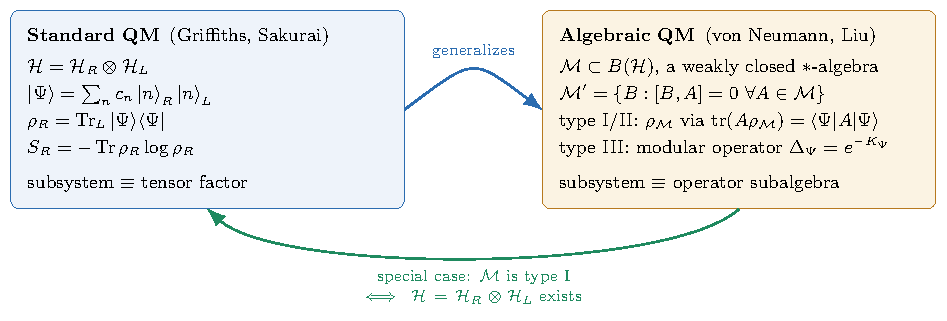
\includegraphics[width=0.92\textwidth]{figs/fig_roadmap.pdf}
\caption{The foundational paradigm shift: Standard Hilbert space quantum mechanics (left, where subsystems are defined by tensor factors $\HH = \HH_R \otimes \HH_L$) generalizes to Algebraic Quantum Mechanics (right, where subsystems are defined by operator subalgebras $\M \subset B(\HH)$). Type I algebras represent the familiar special case where a tensor product factorization exists.}
\label{fig:roadmap}
\end{figure}

\subsection{The Conceptual Bridge: From Wavefunctions to Density Matrices to Algebraic States}

To understand why the algebraic framework of this paper is so natural, it is essential to trace how our concept of a ``quantum state'' evolves as we move from simple undergraduate quantum mechanics to open systems, quantum field theory, and quantum gravity.

\begin{enumerate}[leftmargin=*]
\item \textbf{Level 0: The Pure Wavefunction $\psi(x) = \braket{x|\Psi}$.}
In textbook quantum mechanics, the fundamental entity is a state vector $\ket\Psi \in \HH$ evolving according to the Schr\"odinger equation. Probabilities are given by the Born rule $P(x) = |\psi(x)|^2$. This description assumes a \emph{closed, isolated universe} where an experimenter has unrestricted access to measure arbitrary operators across the entire system.

\item \textbf{Level 1: The Density Matrix $\rho(x, x')$ and Phase Space ($x_c, x_q$).}
When a system interacts with an unobserved environment or thermal bath, pure states give way to density operators $\rho = \sum_k p_k \ket{\psi_k}\bra{\psi_k}$. In the continuous position basis $\rho(x, x') = \braket{x|\rho|x'}$, it is physically illuminating to transform to Keldysh variables:
\[
x_c \equiv \frac{x + x'}{2} \quad \text{(classical midpoint coordinate)}, \qquad x_q \equiv x - x' \quad \text{(quantum coherence coordinate)}.
\]
The diagonal slice $x_q = 0$ encodes classical probabilities $P(x_c) = \rho(x_c, x_c)$, while non-zero $x_q$ tracks off-diagonal quantum interference. Fourier transforming along the quantum coordinate gives the \textbf{Wigner quasi-probability distribution}:
\[
W(x_c, p_q) = \int_{-\infty}^\infty \dd x_q\, e^{-i p_q x_q}\, \rho\!\left(x_c + \tfrac{x_q}{2},\, x_c - \tfrac{x_q}{2}\right) .
\]
While this bridges classical stochastic physics and quantum mechanics, it still fundamentally presumes that the global Hilbert space factorizes as $\HH = \HH_{\rm system} \otimes \HH_{\rm environment}$.

\item \textbf{Level 2: The Physical Limitation of Observers.}
In realistic experiments, no observer has access to the full density matrix on all of $\HH$. An observer is equipped with a restricted apparatus or confined to a spatial subregion $R$. If an observer can only measure a restricted set of observables $\M$, attempting to describe their subsystem via global pure kets produces severe mathematical pathologies (for instance, the standard relative entropy $D(\rho\|\sigma) = \Tr(\rho\log\rho - \rho\log\sigma)$ formally blows up to $+\infty$ whenever $\sigma$ is pure, because it assumes the observer is free to measure arbitrary non-commuting projection operators across the universe).

\item \textbf{Level 3: The Algebraic State $\omega: \M \to \mathbb{C}$.}
In algebraic quantum mechanics (von Neumann, Haag, and Liu), we discard the assumption that a fixed global Hilbert space is fundamental. The primary physical object is the \textbf{algebra of accessible observables $\M$}. A \textbf{state} $\omega$ is simply a positive linear functional assigning expectation values to operators:
\[
\omega(A) = \langle A \rangle_\omega, \qquad \omega(\id) = 1, \quad \omega(A^\dagger A) \ge 0 \quad \forall A \in \M.
\]
The Hilbert space $\HH_\omega$ and state vector $\ket{\Omega_\omega}$ are not postulated in advance; they are \textbf{dynamically manufactured} from the algebraic state $\omega$ via the Gelfand--Naimark--Segal (GNS) construction:
\[
\omega(A) = \braket{\Omega_\omega | \pi_\omega(A) | \Omega_\omega} .
\]
\end{enumerate}

\begin{keyresult}
\textbf{The Conceptual Takeaway:} The wavefunction $\psi(x)$ is not a universal container of physical reality; it is merely one specific GNS representation of an algebraic state $\omega$ on a Type I algebra. When moving to the thermodynamic limit ($N\to\infty$), local subregions in QFT, or semiclassical black holes, the Hilbert space tensor factorization dissolves, but the algebraic state $\omega$ remains exact, rigorous, and well-defined.
\end{keyresult}

\subsection{Why the ordinary quantum-mechanical definition of ``subsystem'' isn't good enough}

To see why a new mathematical tool is needed at all, you have to see precisely where the old one breaks. The
old tool is the one from every quantum mechanics course: given a system built out of two pieces, $R$ and $L$
(read them as ``right'' and ``left,'' or ``region'' and its complement — any bipartition), the Hilbert space of
the whole system factors as a tensor product,
\[
\HH = \HH_R\otimes\HH_L .
\]
Concretely, if $\HH_R$ has orthonormal basis $\{\ket i_R\}$ and $\HH_L$ has orthonormal basis
$\{\ket a_L\}$, then $\HH_R\otimes\HH_L$ is spanned by all the pairs $\ket i_R\ket a_L$, and a general state of
the joint system is a sum $\ket\Psi = \sum_{ia} c_{ia}\ket i_R\ket a_L$ for some array of complex numbers
$c_{ia}$ (Liu's eq.~1.1, written with a continuous or more general index set — the idea is identical). This
state is called \textbf{entangled} exactly when the array $c_{ia}$ cannot be written as a simple product
$c_{ia}=\psi_i\chi_a$ for two smaller arrays $\psi_i,\chi_a$ — i.e., when it doesn't factor into ``something
about $R$'' times ``something about $L$.''

Everything about entanglement that you already know — the reduced density matrix
$\rho_R\equiv\Tr_L\ket\Psi\!\bra\Psi$ (tracing out, i.e., summing over, the $L$ degrees of freedom), the
entanglement entropy $S_R=-\Tr_R(\rho_R\log\rho_R)$, the R\'enyi entropies, the relative entropy — every one
of these formulas (Liu's eqs.~2.2--2.4) is built directly on top of the tensor factorization
$\HH=\HH_R\otimes\HH_L$. If that factorization doesn't exist, none of these formulas can even be written down,
because there is no $\HH_L$ to trace over and no well-defined ``$R$-part'' of the state to extract. The whole
apparatus of entanglement entropy that you learned collapses at the first step, not because it gives a wrong
answer, but because it has no answer to give.

The paper's central claim — the one that everything else builds on — is that this factorization genuinely
fails to exist, not as some exotic mathematical pathology, but in exactly the situations that matter most:
gauge theories, many-body systems in a thermodynamic (infinite-volume or infinite-$N$) limit, quantum field
theories cut into two regions by a surface, and — the case this paper cares about most — the large-$N$ limit
of a holographic boundary theory. Section~II.A of the paper (and this companion's next section) works through
three concrete examples of exactly how and why it fails. It is worth working through the second of these three
examples slowly and completely here, in Sec.~I, because it is the single example every later section in the
paper keeps coming back to.

\subsection{The example that carries the whole paper: infinitely many entangled qubit pairs}

Take a single pair of qubits, one belonging to $R$ and one to $L$, prepared in the state
\[
\ket{\phi_\theta} = \cos\theta\,\ket0_R\ket0_L + \sin\theta\,\ket1_R\ket1_L , \qquad \theta\in(0,\pi/4] .
\]
This is completely standard material: it's a partially entangled pair (maximally entangled exactly at
$\theta=\pi/4$, where the coefficients become equal, $\tfrac1{\sqrt2}$ each — this is a Bell pair). You could
build this in a lab tomorrow with two photons or two trapped ions. Nothing about a single pair is
mysterious.

To see the reduced density matrix explicitly, write out the full $4\times4$ density operator for the pure pair:
\[
\ket{\phi_\theta}\bra{\phi_\theta} = \cos^2\theta\ket{00}\bra{00} + \cos\theta\sin\theta\ket{00}\bra{11} + \sin\theta\cos\theta\ket{11}\bra{00} + \sin^2\theta\ket{11}\bra{11} .
\]
Now take the partial trace over subsystem $L$ by summing over the orthonormal basis $\{\ket0_L, \ket1_L\}$:
\begin{align*}
\rho_R &\equiv \Tr_L\ket{\phi_\theta}\bra{\phi_\theta} = {}_L\braket{0|\phi_\theta}\bra{\phi_\theta}0\rangle_L + {}_L\braket{1|\phi_\theta}\bra{\phi_\theta}1\rangle_L \\
&= \cos^2\theta\,\ket0_R\bra0_R + \sin^2\theta\,\ket1_R\bra1_R = \begin{pmatrix} \cos^2\theta & 0 \\ 0 & \sin^2\theta \end{pmatrix} .
\end{align*}
Because $\rho_R$ is already diagonal, its operator logarithm is obtained by taking the logarithm of each eigenvalue along the diagonal:
\[
\log\rho_R = \begin{pmatrix} \log(\cos^2\theta) & 0 \\ 0 & \log(\sin^2\theta) \end{pmatrix} .
\]
The single-pair von Neumann entanglement entropy follows immediately by evaluating the trace:
\begin{align*}
s_1(\theta) &= -\Tr_R(\rho_R\log\rho_R) = -\left[ \cos^2\theta\log(\cos^2\theta) + \sin^2\theta\log(\sin^2\theta) \right] .
\end{align*}
Evaluating at key points:
\begin{itemize}
\item For the maximally entangled Bell pair at $\theta=\pi/4$, $\cos^2(\pi/4)=\sin^2(\pi/4)=1/2$, yielding
\[
s_1(\pi/4) = -\left[ \tfrac12\log(\tfrac12) + \tfrac12\log(\tfrac12) \right] = \log 2 \approx 0.693147\text{ nats} \quad (= 1\text{ bit}).
\]
\item In the weakly entangled limit $\theta \to 0$, with $\sin^2\theta \approx \theta^2$ and $\cos^2\theta \approx 1 - \theta^2$:
\[
s_1(\theta) \approx -(1-\theta^2)\log(1-\theta^2) - \theta^2\log(\theta^2) \approx \theta^2(1 - 2\log\theta) \to 0 .
\]
\end{itemize}

Now take $N$ independent copies of this pair — $N$ separate two-qubit systems, each prepared the same way —
and glue them together into one big state:
\[
\ket{\Phi_\theta} = \ket{\phi_\theta}_1\otimes\ket{\phi_\theta}_2\otimes\cdots\otimes\ket{\phi_\theta}_N .
\]
Group all the $R$-qubits together into ``the $R$ system'' and all the $L$-qubits into ``the $L$ system.'' At
any finite $N$, this is still completely mundane: $\HH_R=(\mathbb C^2)^{\otimes N}$ is a $2^N$-dimensional
Hilbert space, $\HH=\HH_R\otimes\HH_L$ obviously factors (it's built by construction as a tensor product), and
the total reduced density operator is the $N$-fold tensor product $\rho_R^{(N)} = \rho_R^{\otimes N}$. By the additivity of von Neumann entropy across independent tensor products ($S(\rho_1 \otimes \rho_2) = S(\rho_1) + S(\rho_2)$), the $N$-pair total is exactly
\[
S_R^{(N)} = N\, s_1(\theta) .
\]
At $\theta=\pi/4$, $s_1(\pi/4)=\log2\approx0.693$. So for $N=1$, $S_R=0.693$; for $N=10$, $S_R=6.93$; for
$N=1000$, $S_R=693$. There is nothing subtle about any single one of these numbers — you could verify each
one by direct computation. The interesting physics only shows up once you ask what happens as
$N\to\infty$ while insisting on staying inside the set of states a real, finite-energy experiment could
actually reach.

\subsubsection*{Restricting to finite energy}

Suppose a Hamiltonian $H=H_R+H_L$ assigns an energy cost to flipping any given pair away from its ground
state — concretely, Liu takes $H_R=H_L=f\sum_{i=1}^N Z_i$ (footnote~4 of the paper), where $Z_i$ is the Pauli
$Z$ operator on the $i$-th spin, $Z=\ket0\bra0-\ket1\bra1$, and $f>0$ is some fixed energy scale. On a single pair in state $\ket{\phi_\theta}$, the expectation value of the single-site Pauli operator is
\[
\braket{\phi_\theta|Z_R|\phi_\theta} = \cos^2\theta\braket{0|Z|0} + \sin^2\theta\braket{1|Z|1} = \cos^2\theta - \sin^2\theta = \cos(2\theta) .
\]
Applying a spin-flip operator $X_i = \ket0\bra1 + \ket1\bra0$ to site $i$ exchanges $\ket0 \leftrightarrow \ket1$, replacing $Z_i$ with $-Z_i$ and incurring an energy cost of
\[
\Delta E_i = \braket{\Phi_\theta | X_i (f Z_i) X_i | \Phi_\theta} - \braket{\Phi_\theta | f Z_i | \Phi_\theta} = 2f \cos(2\theta) > 0 .
\]
A \textbf{finite-energy state} built on top of the reference state $\ket{\Phi_\theta}$ is one you reach by flipping only a finite number $k < \infty$ of the $N$ spins, with total excitation energy $\Delta E = 2k f \cos(2\theta) < \infty$. Flipping infinitely many spins costs $\Delta E \to \infty$, and no physical experiment supplies infinite energy.

Here is the key computation, which is worth actually doing rather than just asserting. Suppose you want to
fully disentangle $R$ from $L$ — to end up in some product state $\ket\psi_R\otimes\ket\chi_L$ with zero
entanglement entropy — starting from $\ket{\Phi_\theta}$. Because entanglement entropy is additive over the
$N$ independent pairs, and each pair individually carries entropy $s_1(\theta)>0$, disentangling requires
individually addressing (in the limiting case, individually flipping) every single one of the $N$ pairs. There
is no shortcut: you cannot remove the entanglement of pair number $573{,}241$ without doing something to pair
number $573{,}241$ specifically. As $N\to\infty$, the number of pairs you'd need to touch goes to infinity,
and so — since each one costs a fixed, nonzero amount of energy to address — does the energy required. This is
the precise content of Liu's statement (i) on p.~9: \emph{unentangling the $R$ and $L$ subsystems would
require flipping an infinite number of spins, thus costing infinite energy.} A margin note in one copy of the
paper clarifies exactly what ``unentangling'' means operationally here: it is \emph{applying some further
joint operation to $R$ and $L$ together that transforms the state back into a tensor product of individual
qubit states} — not something mysterious, just an ordinary (if very large) quantum operation, which happens to
be unavailable at finite energy in this limit.

Three consequences follow, and it is worth listing them separately because they are logically distinct facts,
not restatements of one another.

\begin{enumerate}
\item \textbf{Every finite-energy state has infinite entanglement.} Take any state you can reach from
$\ket{\Phi_\theta}$ by flipping finitely many spins. It still has all but finitely many of its $N$ pairs
sitting in the original entangled configuration, so its total entanglement entropy is still (a finite
correction away from) $N\,s_1(\theta)\to\infty$. There is no unentangled, or even weakly entangled, state
anywhere in the finite-energy sector — every physically reachable state is maximally, infinitely entangled
across $R|L$.

\item \textbf{The Hilbert space itself refuses to factor.} A tensor factorization $\HH=\HH_R\otimes\HH_L$ is,
among other things, a promise that unentangled product states $\ket\psi_R\otimes\ket\chi_L$ exist inside
$\HH$ — they're the simplest vectors you can write down once you have the factorization. If every
finite-energy state is infinitely entangled, no such product state can be a finite-energy state, so the
finite-energy Hilbert space $\HH_{\Phi_\theta}$ (built by completing the span of all finite-energy excitations
of $\ket{\Phi_\theta}$) simply does not contain any vectors that look like $\ket\psi_R\otimes\ket\chi_L$. Since
that is exactly what a tensor factorization requires, $\HH_{\Phi_\theta}$ cannot be written as
$\HH_R\otimes\HH_L$ for any sensible choice of $\HH_R,\HH_L$. This isn't a failure to find the right
factorization — the paper's stronger claim, which takes some sitting with, is that $\HH_{\Phi_\theta}$ is not
even a \emph{separable} Hilbert space (one with a countable basis) in the strict $N\to\infty$ limit; it's a
much larger, less tame object, and the usual tools of quantum mechanics (which all assume separability) don't
apply to it directly at all.

\item \textbf{Different values of $\theta$ live in different worlds.} Compare $\ket{\Phi_{\theta}}$ and
$\ket{\Phi_{\theta'}}$ for $\theta\ne\theta'$. As $N\to\infty$, the amount of entanglement (hence, by the same
energy argument, the amount of energy) separating these two states diverges. They are not close to each other,
and no finite-energy operation connects one to the other. In the strict limit, they are best thought of as
two entirely separate theories that happen to share a Hamiltonian's functional form, rather than two states of
one single theory.
\end{enumerate}

If you want to see the size of these numbers directly rather than just the qualitative trend, here is the
$\theta=\pi/4$ case computed explicitly at a few values of $N$ (each entry is exact, not approximate — it
follows immediately from additivity of entropy over the $N$ independent, identical pairs):

\begin{center}
\begin{tabular}{ccccc}
\toprule
$N$ & $1$ & $10$ & $100$ & $10{,}000$ \\
\midrule
$\dim\HH_R^{(N)}=2^N$ & $2$ & $1024$ & $\approx1.3\times10^{30}$ & astronomically large \\
$S_R^{(N)}=N\log2$ & $0.693$ & $6.93$ & $69.3$ & $6931$ \\
\bottomrule
\end{tabular}
\end{center}
There is nothing hidden in this table — every entry is just $N\log2$, computed directly — but seeing the
entropy grow without bound while the dimension of $\HH_R^{(N)}$ explodes is the concrete picture behind the
abstract statement ``$\HH_{\Phi_\theta}$ is not separable.''

\begin{figure}[htbp]
\centering
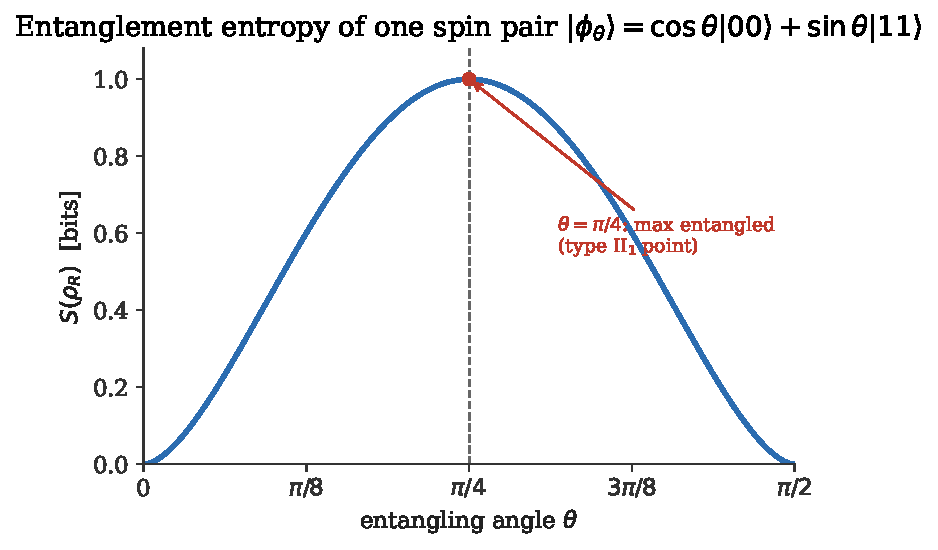
\includegraphics[width=0.75\textwidth]{figs/fig_qubit_entropy.pdf}
\caption{The single-pair entanglement entropy $s_1(\theta) = -\cos^2\theta\log(\cos^2\theta) - \sin^2\theta\log(\sin^2\theta)$ as a function of the mixing angle $\theta \in (0, \pi/4]$. The entropy peaks at the maximally entangled Bell state $\theta = \pi/4$ ($s_1 = \log 2 \approx 0.693$) and vanishes smoothly as $\theta \to 0$. For $N$ pairs, the total entropy scales as $S_R^{(N)} = N s_1(\theta) \to \infty$ as $N \to \infty$.}
\label{fig:qubit_entropy}
\end{figure}

\subsection{The other two examples, more briefly}

The paper gives two more examples (Liu's Ex.~1 and Ex.~3, Sec.~II.A), and it's worth knowing what they are
even in outline, because they come back later — the third one especially, since it's the one that actually
applies to quantum field theory and, ultimately, to AdS/CFT.

\textbf{Ex.~1: lattice gauge theory.} A gauge theory (like electromagnetism, or the strong force) has more
mathematical variables than physical degrees of freedom — you write down a field $U_{ij}$ living on each link
of a lattice, but many different configurations of $U_{ij}$ describe the exact same physics, related by
\emph{gauge transformations} $U_{ij}\to V_iU_{ij}V_j^\dagger$. Physical states are required to be invariant
under these transformations. This requirement — not infinite entanglement, a completely different mechanism —
also breaks the naive tensor factorization $\HH=\HH_R\otimes\HH_L$, because the gauge-invariant states don't,
in general, sit inside a product of an $R$-Hilbert-space and an $L$-Hilbert-space; gauge invariance ties the
two together. This example is flagged explicitly as structurally different from the other two, and it comes
back in Sec.~III.C as a comparatively mild complication (it just adds a classical label — which
gauge/superselection sector you're in — on top of an otherwise ordinary tensor-product story), rather than the
deep, qualitative break that Ex.~2 and Ex.~3 represent.

\textbf{Ex.~3: a quantum field theory cut in half.} Take a relativistic quantum field theory (a scalar field,
say) and split space into two halves, $R=\{x>0\}$ and $L=\{x<0\}$. A quantum field has infinitely many degrees
of freedom packed into any interval of space, however small — informally, a value (or a mode) at every point.
Right at the cutting surface $x=0$, there are infinitely many field degrees of freedom on the $R$ side pressed
arbitrarily close to infinitely many on the $L$ side, all coupled to their immediate neighbors, and this
produces infinite entanglement across the cut in \emph{any} finite-energy state — including the vacuum, the
lowest-energy state there is. This is the field-theory version of exactly the mechanism in Ex.~2 (infinitely
many independent contributions to the entanglement, each one small but adding up to an infinite total), and it
shows up concretely as a divergence: computing the entanglement entropy of the region $R$ with a short-distance
cutoff $\epsilon$ (imagine putting the theory on a lattice with spacing $\epsilon$, which makes everything
finite and well-defined, then asking what happens as $\epsilon\to0$) gives
\[
S_R(\epsilon) = b\,\frac{\mathrm{Area}(\partial R)}{\epsilon^{d-2}} + \cdots, \qquad \epsilon\to0,
\]
(Liu's eq.~2.7) where $\partial R$ is the surface separating $R$ from $L$, $d$ is the spacetime dimension, and
$b$ is some positive, theory-dependent constant. The entropy diverges as the cutoff is removed, and it diverges
in a very specific way — proportional to the \emph{area} of the cutting surface, not its volume. This
``area-law divergence'' is one of the most robust, model-independent facts in quantum field theory (it shows
up in essentially every explicit calculation, from free fields to interacting ones), and this paper's claim is
that it is the direct field-theoretic shadow of exactly the same Hilbert-space-non-factorization phenomenon
as the spin-pair example above — made completely precise later, in Sec.~IV.D, using the language of von
Neumann algebra types.

\begin{figure}[htbp]
\centering
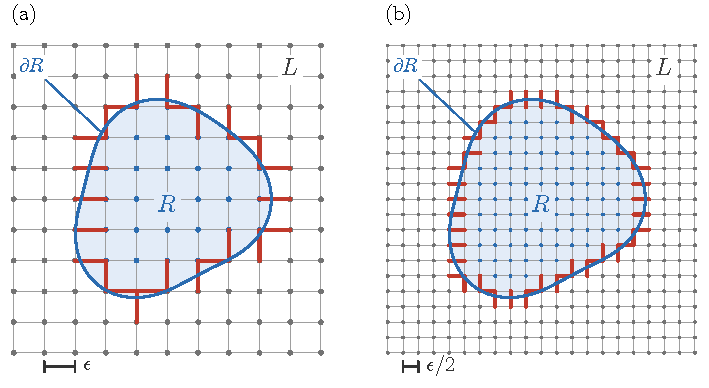
\includegraphics[width=0.75\textwidth]{figs/fig_area_law.pdf}
\caption{The UV area-law divergence of entanglement entropy in quantum field theory: dividing space across a boundary $\partial R$ couples short-distance modes across the cut with UV cutoff $\epsilon$. The leading entanglement entropy diverges as $S_R \sim \mathrm{Area}(\partial R)/\epsilon^{d-2}$, reflecting the infinite entanglement of the underlying Type $\mathrm{III}_1$ local algebra.}
\label{fig:area_law}
\end{figure}

\subsection{Explicit Derivation: Why the Continuum QFT Hilbert Space Cannot Factorize}
\label{sec:qft_nonfactorization_derivation}

Because the claim that ``$\HH \ne \HH_R \otimes \HH_L$ in continuum QFT'' is so fundamental to everything that follows, it is illuminating to derive this result explicitly using nothing more advanced than the quantum mechanics of coupled harmonic oscillators.

\subsubsection*{1. The Hamiltonian and the spatial gradient coupling}

Consider a free, real scalar field $\phi(t, \vec x)$ with mass $m$ in $d$ spacetime dimensions ($d-1$ spatial dimensions). The field Hamiltonian on a constant-time Cauchy slice is
\begin{equation}
H = \int \dd^{d-1}x \left[ \frac{1}{2}\pi(\vec x)^2 + \frac{1}{2}\big(\vec\nabla\phi(\vec x)\big)^2 + \frac{1}{2}m^2\phi(\vec x)^2 \right],
\label{eq:scalar_hamiltonian_continuum}
\end{equation}
where $\pi(\vec x)$ is the canonical momentum field satisfying $[\phi(\vec x), \pi(\vec y)] = i\delta^{(d-1)}(\vec x - \vec y)$.

Now divide space into two halves by a planar boundary at $x = 0$:
\[
R = \{ (x, \vec x_\perp) : x > 0 \}, \qquad L = \{ (x, \vec x_\perp) : x < 0 \},
\]
where $\vec x_\perp = (x^2, \dots, x^{d-1})$ denotes the $(d-2)$ spatial coordinates parallel to the entangling surface $\partial R$.

To isolate the physics right at the boundary, we discretize the perpendicular $x$-direction on a spatial lattice with lattice spacing $\epsilon$, while Fourier-transforming the continuous transverse coordinates $\vec x_\perp$ into transverse momentum modes $\vec k_\perp$:
\[
\phi(x, \vec x_\perp) = \int \frac{\dd^{d-2}k_\perp}{(2\pi)^{d-2}} \, \widetilde\phi(x, \vec k_\perp) \, e^{i \vec k_\perp \cdot \vec x_\perp} .
\]
For each transverse momentum mode $\vec k_\perp$, the Hamiltonian decomposes into an independent 1D chain of coupled harmonic oscillators with effective mass parameter
\begin{equation}
M^2 \equiv m^2 + |\vec k_\perp|^2 .
\label{eq:effective_mass_transverse}
\end{equation}
On the lattice in the $x$-direction, the continuous field becomes discrete site operators $\phi_j(\vec k_\perp) \equiv \widetilde\phi(j\epsilon, \vec k_\perp)$ with conjugate momenta $\pi_j(\vec k_\perp)$, where $j = \dots, -2, -1$ lies in $L$ and $j = 0, 1, 2, \dots$ lies in $R$.

The spatial gradient in the direction perpendicular to the boundary is discretized via finite differences:
\begin{equation}
\int \dd x \, \frac{1}{2}\left(\frac{\partial\phi}{\partial x}\right)^2 \;\longrightarrow\; \sum_j \frac{\epsilon}{2} \left( \frac{\phi_{j+1} - \phi_j}{\epsilon} \right)^2 = \sum_j \frac{1}{2\epsilon} (\phi_{j+1} - \phi_j)^2 .
\label{eq:lattice_gradient_sum}
\end{equation}
Notice the crucial interaction link directly straddling the entangling cut between site $j = -1$ (the closest site in $L$) and site $j = 0$ (the closest site in $R$):
\begin{equation}
H_{\rm cut} = \frac{1}{2\epsilon} (\phi_0 - \phi_{-1})^2 = \frac{1}{2\epsilon} (\phi_R - \phi_L)^2 ,
\label{eq:h_cut_interaction}
\end{equation}
where for clarity we define $\phi_R \equiv \phi_0$ and $\phi_L \equiv \phi_{-1}$.

\subsubsection*{2. The two-oscillator subsystem across the entangling cut}

To see the mechanism with complete clarity, isolate this two-mode system across the interface. The Hamiltonian for these two adjacent oscillators is
\begin{equation}
H_{\rm pair} = \frac{1}{2}\pi_R^2 + \frac{1}{2}\pi_L^2 + \frac{1}{2}M^2(\phi_R^2 + \phi_L^2) + \frac{1}{2\epsilon^2}(\phi_R - \phi_L)^2 .
\label{eq:pair_hamiltonian}
\end{equation}
(Rescaling fields to canonical dimensions $\phi \to \phi/\sqrt{\epsilon}$, $\pi \to \pi\sqrt{\epsilon}$ leaves $[\phi, \pi] = i$ and puts the coupling parameter as $k_{\rm cut} = 1/\epsilon^2$).

Because this is a quadratic system, we diagonalize it exactly using normal mode coordinates:
\begin{equation}
\phi_+ \equiv \frac{\phi_R + \phi_L}{\sqrt{2}}, \qquad \phi_- \equiv \frac{\phi_R - \phi_L}{\sqrt{2}} .
\label{eq:normal_mode_coords}
\end{equation}
In terms of $\phi_\pm$, the Hamiltonian decouples into two uncoupled harmonic oscillators:
\begin{equation}
H_{\rm pair} = \left( \frac{1}{2}\pi_+^2 + \frac{1}{2}\omega_+^2 \phi_+^2 \right) + \left( \frac{1}{2}\pi_-^2 + \frac{1}{2}\omega_-^2 \phi_-^2 \right),
\label{eq:decoupled_pair_hamiltonian}
\end{equation}
whose normal mode eigenfrequencies are
\begin{align}
\omega_+ &= M = \sqrt{m^2 + |\vec k_\perp|^2}, \label{eq:omega_plus} \\
\omega_- &= \sqrt{M^2 + \frac{2}{\epsilon^2}} = \sqrt{m^2 + |\vec k_\perp|^2 + \frac{2}{\epsilon^2}} \approx \frac{\sqrt{2}}{\epsilon} \quad \text{as } \epsilon \to 0 . \label{eq:omega_minus}
\end{align}

\subsubsection*{3. Ground state correlations vs. product state correlations}

The ground state of the decoupled system is the product of two Gaussian ground state wavefunctions in the normal coordinates:
\begin{equation}
\Psi_0(\phi_+, \phi_-) = \left( \frac{\omega_+ \omega_-}{\pi^2} \right)^{1/4} \exp\left[ -\frac{1}{2}\omega_+\phi_+^2 - \frac{1}{2}\omega_-\phi_-^2 \right] .
\label{eq:ground_state_normal}
\end{equation}
Transforming back to the physical local fields $\phi_R, \phi_L$ using eq.~\eqref{eq:normal_mode_coords}:
\begin{align}
\Psi_0(\phi_R, \phi_L) &= \left( \frac{\omega_+ \omega_-}{\pi^2} \right)^{1/4} \exp\left[ -\frac{1}{4}(\omega_+ + \omega_-)(\phi_R^2 + \phi_L^2) - \frac{1}{2}(\omega_+ - \omega_-)\phi_R \phi_L \right] .
\label{eq:ground_state_physical}
\end{align}
Notice the cross-coupling term $\frac{1}{2}(\omega_- - \omega_+)\phi_R \phi_L$. Because $\omega_- \approx \sqrt{2}/\epsilon \gg \omega_+$, this cross-term is extraordinarily large. 

In the true vacuum state $\ket\Omega$:
\begin{itemize}
\item The expectation value of the relative difference between the two sides is suppressed:
\begin{equation}
\braket{\Omega | (\phi_R - \phi_L)^2 | \Omega} = 2 \braket{\Omega | \phi_-^2 | \Omega} = \frac{2}{2\omega_-} = \frac{1}{\omega_-} \approx \frac{\epsilon}{\sqrt{2}} .
\label{eq:vacuum_diff_exp}
\end{equation}
\item The gradient energy of the cut in the vacuum state is therefore finite per mode:
\begin{equation}
\braket{\Omega | H_{\rm cut} | \Omega} = \frac{1}{2\epsilon^2} \braket{\Omega | (\phi_R - \phi_L)^2 | \Omega} = \frac{1}{2\epsilon^2} \frac{1}{\omega_-} \approx \frac{1}{2\sqrt{2}\epsilon} .
\label{eq:vacuum_cut_energy}
\end{equation}
This is the standard zero-point vacuum energy density, which is subtracted when computing excitation energies.
\end{itemize}

\subsubsection*{4. The energetic impossibility of unentangled product states}

Now, suppose for the sake of contradiction that the Hilbert space factorizes across the cut:
\[
\HH \stackrel{?}{=} \HH_L \otimes \HH_R .
\]
If this factorization were valid, the Hilbert space must contain unentangled product states of the form
\begin{equation}
\ket{\Psi_{\rm prod}} = \ket{\psi_L} \otimes \ket{\chi_R} \in \HH ,
\label{eq:hypothetical_product_state}
\end{equation}
where $\ket{\psi_L} \in \HH_L$ and $\ket{\chi_R} \in \HH_R$.

In \emph{any} such product state, by the definition of a tensor product, any operator in $L$ and any operator in $R$ have exactly zero quantum covariance:
\begin{equation}
\braket{\Psi_{\rm prod} | \phi_R \phi_L | \Psi_{\rm prod}} = \braket{\chi_R | \phi_R | \chi_R} \braket{\psi_L | \phi_L | \psi_L} .
\label{eq:product_state_covariance_zero}
\end{equation}
For states with zero mean field ($\braket{\phi_R} = \braket{\phi_L} = 0$, as in any symmetric fluctuation), this means $\braket{\phi_R \phi_L}_{\rm prod} = 0$ identically!

Evaluating the expectation value of the difference squared in this product state gives:
\begin{align}
\braket{\Psi_{\rm prod} | (\phi_R - \phi_L)^2 | \Psi_{\rm prod}} &= \braket{\phi_R^2}_{\chi_R} + \braket{\phi_L^2}_{\psi_L} - 2\braket{\phi_R}_{\chi_R}\braket{\phi_L}_{\psi_L} \nonumber \\
&= \braket{\phi_R^2}_{\chi_R} + \braket{\phi_L^2}_{\psi_L} .
\label{eq:prod_diff_squared}
\end{align}
By the Heisenberg uncertainty principle for each oscillator, the fluctuations are bounded strictly from below:
\[
\braket{\phi_R^2}_{\chi_R} \ge \frac{1}{2\Omega_R}, \qquad \braket{\phi_L^2}_{\psi_L} \ge \frac{1}{2\Omega_L} .
\]
In particular, for any state with localized, finite-energy wavepackets of width $\sim \epsilon$, the single-site fluctuation is bounded by the uncoupled ground state scale:
\begin{equation}
\braket{\Psi_{\rm prod} | (\phi_R - \phi_L)^2 | \Psi_{\rm prod}} \ge \frac{1}{2\omega_+} = \frac{1}{2\sqrt{m^2 + |\vec k_\perp|^2}} = \mathcal{O}(1) \quad (\text{finite, independent of } \epsilon) .
\label{eq:prod_fluctuation_lower_bound}
\end{equation}
Notice the striking difference between eq.~\eqref{eq:vacuum_diff_exp} and eq.~\eqref{eq:prod_fluctuation_lower_bound}:
\begin{itemize}
\item In the entangled vacuum, $\braket{(\phi_R - \phi_L)^2} \sim \mathcal{O}(\epsilon) \to 0$ as the lattice spacing vanishes.
\item In \emph{any} product state, $\braket{(\phi_R - \phi_L)^2} \ge \mathcal{O}(1)$ remains strictly finite as $\epsilon \to 0$, because the absence of entanglement prevents the field values on adjacent sides from fluctuating in lockstep!
\end{itemize}

Now compute the gradient energy across the boundary link in this product state:
\begin{equation}
\braket{\Psi_{\rm prod} | H_{\rm cut} | \Psi_{\rm prod}} = \frac{1}{2\epsilon^2} \braket{\Psi_{\rm prod} | (\phi_R - \phi_L)^2 | \Psi_{\rm prod}} \ge \frac{1}{4\epsilon^2 \sqrt{m^2 + |\vec k_\perp|^2}} .
\label{eq:hcut_prod_divergence}
\end{equation}
Subtracting the vacuum zero-point energy (eq.~\eqref{eq:vacuum_cut_energy}), the excess excitation energy required to sever the entanglement of this single transverse mode across the cut is
\begin{equation}
\Delta E_{\rm cut}(\vec k_\perp) = \braket{\Psi_{\rm prod} | H_{\rm cut} | \Psi_{\rm prod}} - \braket{\Omega | H_{\rm cut} | \Omega} \ge \frac{1}{4M\epsilon^2} - \frac{1}{2\sqrt{2}\epsilon} \sim \frac{1}{4M\epsilon^2} > 0 .
\label{eq:delta_e_single_mode}
\end{equation}

\subsubsection*{5. Integration over the entangling surface and the non-factorization theorem}

To obtain the total excitation energy required to prepare the unentangled product state $\ket{\psi_L}\otimes\ket{\chi_R}$ across the entire boundary surface $\partial R$, we integrate $\Delta E_{\rm cut}(\vec k_\perp)$ over all transverse spatial coordinates $\vec x_\perp$, or equivalently over all transverse momentum modes $|\vec k_\perp| \le \Lambda_{\rm UV} \sim 1/\epsilon$:
\begin{align}
\Delta E_{\rm prod} &= \mathrm{Area}(\partial R) \int_{|\vec k_\perp| \le 1/\epsilon} \frac{\dd^{d-2}k_\perp}{(2\pi)^{d-2}} \, \Delta E_{\rm cut}(\vec k_\perp) \nonumber \\
&\ge \mathrm{Area}(\partial R) \int_{|\vec k_\perp| \le 1/\epsilon} \frac{\dd^{d-2}k_\perp}{(2\pi)^{d-2}} \, \frac{1}{4\epsilon^2 \sqrt{m^2 + |\vec k_\perp|^2}} .
\label{eq:total_prod_energy_integral}
\end{align}
Evaluating the radial momentum integral in $d$ spacetime dimensions ($d \ge 3$):
\[
\int_0^{1/\epsilon} k_\perp^{d-3} \frac{\dd k_\perp}{k_\perp} \sim \int_0^{1/\epsilon} k_\perp^{d-4} \dd k_\perp \sim \left(\frac{1}{\epsilon}\right)^{d-3} .
\]
Multiplying by the prefactor $\frac{1}{\epsilon^2}$:
\begin{keyresult}
\begin{equation}
\Delta E_{\rm prod} \ge C \cdot \frac{\mathrm{Area}(\partial R)}{\epsilon^{d-1}} \;\xrightarrow{\;\epsilon \to 0\;} \; +\infty ,
\label{eq:product_state_energy_divergence}
\end{equation}
where $C > 0$ is a strictly positive, theory-dependent geometric constant.
\end{keyresult}

Equation~\eqref{eq:product_state_energy_divergence} is the definitive physical proof of non-factorizability:
\begin{enumerate}
\item \textbf{Infinite energy barrier}: The physical energy required to unentangle a spatial subregion $R$ from its complement $L$ diverges as $\epsilon^{-(d-1)}$ in the continuum limit. Any attempt to enforce a tensor product state requires creating an infinite gradient discontinuity at $\partial R$.
\item \textbf{Expulsion from the physical Hilbert space}: The physical Hilbert space $\HH$ of a continuum quantum field theory consists solely of finite-energy states (mathematically, states in the Fock space or GNS space of the vacuum). Because $\Delta E_{\rm prod} = +\infty$, \emph{no product states exist anywhere within $\HH$}.
\item \textbf{Failure of factorization}: A tensor product $\HH_L \otimes \HH_R$ is, by definition, spanned by product vectors $\ket{\psi_L}\ket{\chi_R}$. Because $\HH$ contains zero product vectors, we reach an inescapable mathematical conclusion:
\begin{equation}
\boxed{\HH \ne \HH_L \otimes \HH_R \quad \text{in any continuum relativistic quantum field theory.}}
\label{eq:non_factorization_conclusion}
\end{equation}
\end{enumerate}

\subsubsection*{6. The algebraic corollary: Type $\mathrm{III}_1$ and the split property}

This energetic divergence explains why local subregions in QFT cannot be described by Type I algebras:
\begin{itemize}
\item If two spatial regions $R_1$ and $R_2$ are separated by a \textbf{finite buffer distance} $\delta > 0$ (so $\text{dist}(R_1, R_2) = \delta$), the gradient energy across the gap is regularized by $\delta$. In that case, an unentangled product state \emph{can} be prepared, but at an energy cost scaling as $\exp(c/\delta^n)$. The mathematical statement that product states exist for strictly separated regions is known in axiomatic QFT as the \textbf{Doplicher--Longo split property}: there exists an intermediate Type I factor $\mathcal{N}$ such that $\M(R_1) \subset \mathcal{N} \subset \M(R_2')'$.
\item However, as the buffer distance is sent to zero ($\delta \to 0$, so the regions touch at a common boundary), the split property collapses, the energy diverges to $+\infty$, and the local algebra $\M(R)$ ceases to be Type I or Type II — it becomes an intrinsically entangled \textbf{Type $\mathrm{III}_1$ factor}.
\end{itemize}

\subsection{The fix: define a subsystem by what you can \emph{do}, not by how you'd \emph{split the Hilbert
space}}

Here is the resolution the paper proposes, and it is worth sitting with how simple the idea actually is
before any formalism gets attached to it. Instead of defining a subsystem $R$ by declaring a factorization
$\HH=\HH_R\otimes\HH_L$ up front, define it operationally: \emph{$R$ is whatever an observer confined to
that subsystem can measure or do.} Concretely, that observer has access to some collection of operators
$\M\subset B(\HH)$ (the set of all bounded operators on the full Hilbert space $\HH$) — every self-adjoint
combination of things their apparatus can measure, and every unitary transformation their apparatus can
apply. Nothing about this definition requires $\HH$ to factor into anything. It only requires that you can
say, of any given operator, whether or not it belongs to the observer's toolkit.

This reframing costs nothing in the ordinary case (when $\HH=\HH_R\otimes\HH_L$ genuinely does exist, the
natural choice $\M=B(\HH_R)\otimes\id_L$ — every operator acting only on $R$ — recovers exactly the familiar
picture, as you'll see made precise in the next section), and it costs nothing in the broken case either,
because ``the set of operators an $R$-observer can apply'' is a perfectly sensible, well-defined thing to talk
about even when there's no factorization for it to come from. You lose nothing and gain a definition that
survives exactly the cases where the old one dies.

Naming what kind of mathematical object $\M$ should be — closed under sums, products, and the operation of
taking a Hermitian conjugate, plus some notion of being closed under limits — is precisely what a
\textbf{von Neumann algebra} is, and pinning down exactly which notion of ``limit'' is the right one (there
turn out to be two inequivalent choices, and the difference matters enormously) is the entire content of the
next section, Sec.~II.

This is, historically, not a new invention grafted onto quantum mechanics from outside. In the late 1920s and
early 1930s, John von Neumann — one of the people who built the mathematical foundations of quantum mechanics
in the first place, the same person behind the ``Dirac--von Neumann axioms'' you may have seen stated in
Sakurai — worked out, together with Francis Murray, a complete classification of exactly these kinds of
operator algebras. For decades this classification lived mostly inside pure mathematics. The claim of this
paper (built on work going back to Rehren in the 1990s, and developed intensively since roughly 2021 by
Leutheusser, Liu, and others) is that this same 1930s classification, when applied to the algebra $\M$ of an
observer's accessible operators, is \emph{exactly} a classification of how entangled that observer's
subsystem is with everything they cannot access — turning an abstract piece of 1930s functional analysis into
a working tool for 2020s quantum gravity.

\subsection{Two organizing claims, and how seriously to take them at this stage}

The paper states its two central claims very early (its eq.~1.3 and the paragraph after it), and it is useful
to know, right at this stage, exactly how much has been established when you first read them, versus how much
is being promised for later. Restated:

\begin{center}
\emph{Classifying von Neumann algebras} $\;\longleftrightarrow\;$ \emph{classifying broad types of
entanglement.}
\end{center}

and, going beyond this broad classification, finer tools from the same theory (modular theory, covered in
Sec.~IV, and the crossed product, covered in Sec.~V) are claimed to give access to much sharper entanglement
information than the broad type alone.

At the point in the paper where these claims first appear, they are \emph{stated}, not yet demonstrated. Don't
mistake the double-headed arrow above for a formal theorem with a name and a citation — it isn't one. It's a
dictionary that gets built up, entry by entry, over Secs.~III and IV: each von Neumann algebra type (I, then
II, then the various subtypes of III) is matched, on specific worked examples, to a specific qualitative
pattern of entanglement between a subsystem and its complement. By the time you finish Sec.~IV you will have
seen this correspondence demonstrated concretely enough, on examples you can check by hand, that the arrow in
eq.~1.3 will feel earned rather than asserted. That is exactly the arc this companion follows too — the
promise made here in Sec.~I is redeemed piece by piece, not all at once.

Similarly, the deeper claim that entanglement structure is what \emph{builds} bulk spacetime geometry — the
subregion-subalgebra duality that gives this paper its title — is motivated here by pointing at the
Ryu--Takayanagi formula and the broader ``entanglement builds geometry'' literature (Van~Raamsdonk
\cite{VanRaamsdonk}, Maldacena--Susskind \cite{MaldacenaSusskind}), but the actual mechanism — \emph{why} a
boundary algebra of a specific type turns out to be identical, not just related, to a bulk causal region's
algebra of observables — isn't built until Sec.~VII. Reading Sec.~I as ``a map of where we're going and why
people believe it's worth going there,'' rather than as a self-contained argument, is the right way to read
it; that's genuinely all a paper's introduction can do.

\subsection{Sec.~I.A: the plan of the article, translated}

The paper's own plan (p.~6) splits its ten sections into two halves. It's worth restating in a way that says
\emph{why} the split falls where it does, since the reason is itself informative about how the argument is
built.

\textbf{Secs.~II--V: the mathematics, with no gravity or holography anywhere in sight.} This half is pure
operator-algebra theory, developed using only ordinary, finite-dimensional-friendly quantum mechanics
examples (mostly the entangled-spin-pair system from above). Sec.~II lays down what a von Neumann algebra is
and how they're classified. Secs.~III and IV show, type by type, how that classification tracks entanglement
structure — Sec.~III handles the ``easy'' types (I and II, where a density matrix and an entropy can still be
defined), and Sec.~IV handles type III, which cannot be tamed by a density matrix at all and needs an entirely
new tool (Tomita--Takesaki modular theory) to say anything quantitative about it. Sec.~V introduces the
\emph{crossed product}, a construction that takes a type III algebra and, by literally attaching an auxiliary
quantum clock to it, produces a new, better-behaved type II algebra out of it — a purely algebraic trick at
this stage, with no physical motivation given yet, but one that turns out (starting in Sec.~IX) to be exactly
what a real physical observer, carrying a real physical clock, is doing to gravitational observables.

\textbf{Secs.~VI--IX: applying all of that machinery to quantum gravity.} Sec.~VI sets up the large-$N$
algebraic formulation of AdS/CFT itself. Sec.~VII introduces subregion-subalgebra duality — the paper's
central physics claim, that a bulk spacetime region and a specific boundary operator algebra are literally the
same object, described in two languages — and uses it to reformulate entanglement-wedge and causal-wedge
reconstruction (ideas you may already have encountered in AdS/CFT courses) in this new algebraic language.
Sec.~VIII shows how bulk causal structure, horizons, and even the question of whether two disconnected
boundary theories are joined by a wormhole, can all be read directly off the type and commutant structure of
boundary algebras, with no bulk metric assumed anywhere. Sec.~IX builds simple, fully solvable toy models
(observers with real physical clocks, crossed by the modular group exactly as in Sec.~V) that reproduce black
hole and de~Sitter entropy from nothing but this operator-algebraic machinery.

\subsection{Sec.~I.B: conventions and notation, explained rather than just listed}

This short subsection (p.~8 of the paper) is easy to skim past, but every single item in it gets used, without
further comment, dozens of times later — so it's worth actually understanding each one now rather than
looking it up under pressure in Sec.~VII.

\begin{itemize}
\item \textbf{Large $N$ vs.\ finite $N$.} ``Large-$N$'' (equivalently $G_N\to0$) means doing a perturbative
expansion in powers of $1/N$ — you can keep more than just the very first (leading) term, but you're still
fundamentally treating $1/N$ as a small parameter you expand in, the same way you'd do ordinary perturbation
theory in quantum mechanics. ``Finite $N$'' (finite $G_N$) means the opposite: treating $N$ (or $G_N$) as an
honest, fixed number, with no expansion at all — the genuinely nonperturbative, full quantum-gravity regime.
Most of this paper works at large $N$; finite-$N$ questions are the hardest open problems, touched on mainly
in Secs.~VII.F and IX.D.

\item \textbf{$\HH$, $B(\HH)$, and boundedness.} $\HH$ is a Hilbert space (a complex vector space with an
inner product, complete under the norm that inner product defines — the same notion you already know from
ordinary quantum mechanics, just possibly infinite-dimensional). $B(\HH)$ is the set of \emph{bounded}
operators on $\HH$: an operator $A$ is bounded if there's some finite number $c$ such that $\|A\ket\psi\|\le
c\|\ket\psi\|$ for every vector $\ket\psi\in\HH$ — informally, $A$ never stretches a vector's length by more
than a fixed factor, no matter which vector you feed it. Ordinary finite matrices are automatically bounded.
Some familiar quantum-mechanical operators are \emph{not} bounded — position $\hat x$ and momentum $\hat p$ on
a particle on a line, for instance, can make $\|A\ket\psi\|/\|\ket\psi\|$ as large as you like by choosing
$\ket\psi$ spread out far enough, or oscillating fast enough. The paper sidesteps this by simply restricting
attention to bounded operators throughout, and noting that in field theory any operator you actually care
about can be suitably smeared/regularized to become bounded (e.g., $e^{i\hat x}$ is bounded even though
$\hat x$ itself is not). This restriction is not a loss of generality worth worrying about; it's a standard
technical convenience that lets the norm-based definitions below (Sec.~II.B.1) work cleanly.

\item \textbf{$\id$} is the identity operator — ``do nothing.''

\item \textbf{$\widetilde J^\pm(Y)$: causal future and past.} For a region $Y$ in a spacetime, $\widetilde
J^+(Y)$ is the set of every point that can be reached from some point of $Y$ by a future-directed causal
curve — a path that never moves faster than light and always moves forward in time. Physically: everything $Y$
could possibly send a signal to, given unlimited time. $\widetilde J^-(Y)$ is the mirror image: everything
that could have sent a signal to some point of $Y$. (The tilde signals that these are computed in the
\emph{conformal completion} of the spacetime — a technical device, standard in the AdS/CFT literature, that
adds a boundary ``at infinity'' so that causal curves reaching arbitrarily far away are still tracked
properly; you can safely picture ordinary causal future/past for now and revisit the tilde once conformal
compactification actually matters, starting around Sec.~VI.)

\item \textbf{Causal complement (single prime) and causal completion (double prime), on a spacetime region.}
The causal complement $Y'$ of a region $Y$ is everything that is spacelike separated from all of $Y$ — every
point that cannot send or receive a signal to or from any point of $Y$ within the time available; loosely,
``everything $Y$ has absolutely no causal influence on, in either direction.'' The causal completion $Y''$ is
the double complement, $(Y')'$ — and (this is a genuinely important geometric fact, not just a notational
curiosity) $Y''$ is generally \emph{larger} than $Y$ itself: it's the largest region that has exactly the same
causal future and past as $Y$ does. A single point on a Cauchy slice, for instance, has a causal completion
equal to the single point itself (nothing to add), but a spatial region $R$ on a Cauchy slice has a causal
completion equal to its entire \emph{domain of dependence} (defined next) — a genuinely bigger set, extending
into the past and future. This double-prime notation for spacetime regions is deliberately built to echo the
double-prime notation for operator commutants ($\M''$) that you'll meet in the very next section, and the
paper is relying on that echo: causal completion of a region and double-commutant closure of an algebra turn
out, once subregion-subalgebra duality is established in Sec.~VII, to be two faces of the same fact.

\item \textbf{$\bar R$, complement of a spatial region; $\hat R$, domain of dependence.} If $R$ is a subregion
of a single spatial slice (a snapshot of space at one moment), $\bar R$ is just its ordinary set-complement on
that slice — everything on the same slice that isn't in $R$. $\hat R$, the domain of dependence, is a genuinely
spacetime notion built from $R$: it's every spacetime point $p$ such that \emph{every} causal curve through
$p$ — no matter which direction it goes, as long as it never exceeds the speed of light — must cross $R$. This
is exactly the region whose entire future \emph{and} past history is completely determined by data specified
on $R$ alone, which is why it's called the domain of \emph{dependence}: physics inside $\hat R$ depends only on
initial data given on $R$. For $R$ a full spatial slice, $\hat R$ is the entire spacetime. For $R$ a proper
subregion, $\hat R$ is a diamond-shaped region (a \emph{causal diamond}) sitting above and below $R$, bounded
by the light rays that just barely graze the edge of $R$. This shape shows up constantly from Sec.~VI onward;
it's worth actually picturing it once here.

\item \textbf{$\subset$ always means \emph{proper} subset.} A small notational point that matters: whenever
you see $\M_1\subset\M_2$ in this paper, it means $\M_1$ is strictly smaller than $\M_2$ (not equal to it) —
not the more permissive convention (allowing equality) some other texts use for the same symbol.
\end{itemize}

With this vocabulary in hand — bounded operators, causal future/past, causal complement and completion,
domain of dependence — you have everything you need to read the rest of the paper's geometric statements
literally, rather than by pattern-matching to what looks familiar. The next section builds the algebraic
machinery ($C^*$ and von Neumann algebras, states, projections, the type classification, and the GNS
construction that produces a Hilbert space from an algebra) that this section's discussion has been building
toward.

\chapter{Introduction to von Neumann algebras}

Chapter~1 ended with a proposal. A subsystem should be defined not by splitting the Hilbert space, but by
the collection of operators that an observer confined to the subsystem can use. This chapter makes that
proposal precise. By the end of it you will know what kind of mathematical object $\M$ must be, how such
objects are sorted into types, and how a Hilbert space can be \emph{built} from an algebra and a state
instead of being assumed at the start. Most definitions below come with a worked example that uses actual
numbers, often small matrices you can multiply out by hand. The definitions are abstract on first reading,
and watching them act on something small is the quickest way to make them concrete.

\section{Systems with an infinite amount of entanglement (recap)}

Chapter~1 gave three examples: the chain of $N$ Bell pairs, lattice gauge theory, and a quantum field theory
cut in half. They motivate everything in this chapter. The lesson drawn from them was this: a subsystem
should be defined by \emph{which operators are available to act with}, not by how the Hilbert space happens
to split. This chapter turns that idea into a mathematical definition.

\section{Von Neumann algebras as subsystems}

\subsection*{Setting the stage: what a Hilbert space and an operator are, restated carefully}

The new definition is a statement \emph{about} Hilbert spaces and operators. So we first state exactly what
those are. Vague pictures of ``vectors'' and ``operators'' are not precise enough for what follows.

A Hilbert space $\HH$ is a vector space over the complex numbers with two extra properties. First, it has an
inner product $\braket{\cdot|\cdot}$. This is a rule that assigns a complex number $\braket{\xi|\eta}$ to each
pair of vectors. It is linear in the second argument and conjugate-linear in the first, and it satisfies
$\braket{\xi|\xi}\ge0$, with equality only for the zero vector. Second, it is complete. A \emph{Cauchy
sequence} is a sequence of vectors whose terms get arbitrarily close to each other, so that it ``ought to''
converge. Completeness says that every Cauchy sequence really does converge to some vector in $\HH$. For a
spin-$\tfrac12$ particle, $\HH=\mathbb C^2$. Its vectors are pairs of complex numbers $(c_1,c_2)$, usually
written $c_1\ket0+c_2\ket1$. The inner product is the dot product with complex conjugation,
$\braket{\xi|\eta}=\xi_1^*\eta_1+\xi_2^*\eta_2$. A von Neumann algebra needs nothing more exotic than this.
The infinite-dimensional case (a quantum field, say) uses exactly the same definitions, with infinitely many
components instead of two.

An operator $A$ on $\HH$ is a rule that turns vectors into vectors, $A:\HH\to\HH$, and is linear:
$A(c_1\ket{\xi_1}+c_2\ket{\xi_2})=c_1 A\ket{\xi_1}+c_2A\ket{\xi_2}$. On $\mathbb C^2$, every linear operator is
a $2\times2$ matrix, and $A\ket\xi$ is ordinary matrix-vector multiplication. The \textbf{Hermitian
conjugate} (or adjoint) $A^\dagger$ of $A$ is the unique operator with
$\braket{\xi|A\eta}=\braket{A^\dagger\xi|\eta}$ for all $\xi,\eta$. For a finite matrix, this is the familiar
rule ``transpose and complex-conjugate every entry.'' $A$ is \textbf{self-adjoint} (or Hermitian) if
$A=A^\dagger$. Self-adjoint operators are the ones that represent physical observables, because their
eigenvalues are real numbers, the kind of number a measurement can return. $B(\HH)$ denotes the set of
\emph{all} bounded operators on $\HH$. Boundedness was defined in Chapter~1. Informally, a bounded operator
does not stretch the length of any vector by more than some fixed factor.

\subsection*{The new definition of subsystem}

Here is the definition, with every piece spelled out. Suppose you have access to only some subset of
operators, $\M\subset B(\HH)$. This is not everything. It is only what your apparatus, in your location, with
your capabilities, can measure or apply. Let $\ket\Psi\in\HH$ be a state of the full system. Using only $\M$,
you can do two things:
\begin{itemize}
\item compute expectation values $\braket{\Psi|A|\Psi}$ for $A\in\M$, which predict the average reading of a
measurement of $A$ over many repetitions;
\item act on the state, producing $B\ket\Psi$ for $B\in\M$, which changes the system by an operation you have
access to.
\end{itemize}
Whatever $\M$ is, it should be closed under three operations, because an observer with access to $\M$ can
already do each of them. If you can measure or apply $A$ and $B$, you can measure or apply $A+B$ (do both and
add the results) and $AB$ (do one after the other). You can also multiply by complex numbers. And if $A$ is
available, so is $A^\dagger$. For a self-adjoint $A$ this is automatic, since $A^\dagger=A$. In general it
says that your toolkit is closed under taking adjoints. A set closed under sums, products, and adjoints is
called a \textbf{$*$-subalgebra} of $B(\HH)$. The $*$ refers to the adjoint, which mathematics texts often
write as $A^*$ instead of $A^\dagger$. In these notes every $*$-subalgebra is also taken to contain the identity
operator $\id$, which is the operation ``do nothing.''

This alone is not quite enough. We also want $\M$ to be \emph{complete}: if some operator can be approximated
arbitrarily well by elements of $\M$, it should count as an element of $\M$ too. Otherwise the set of things
you have access to would have artificial gaps. Here the story becomes subtle. There are two different,
inequivalent ways to make ``approximated arbitrarily well'' precise, and the choice between them matters a
great deal. The next section explains both.

With this notion of subsystem in hand, the \textbf{complement} of $\M$ is defined to be its commutant,
\[
\M' = \{B\in B(\HH) : BA=AB\ \ \forall A\in\M\} .
\]
One misreading of this definition is common enough to address right away. $\M'$ is \emph{not} the set of
operators that commute \emph{with one another}. It is the set of operators that \emph{each} commute with
\emph{every} element of $\M$. Two operators inside $\M'$ can fail to commute with each other. In fact, when
$\M'$ is a rich enough algebra (the usual case), it contains non-commuting pairs, just as $\M$ does. What
$\M'$ guarantees is only this: acting with anything in $\M'$ produces no interference with any measurement
made using $\M$. That is the operational meaning of ``complement of a subsystem'' here. It is not ``the other
half of a tensor factorization you could point to.'' It is ``everything that, as a matter of algebra, cannot
disturb what $\M$ measures.'' A fuller treatment, with the functional-analysis machinery spelled out, is given
in W.~Thirring's \emph{Quantum Mathematical Physics}. Nothing beyond what is given here is needed for the rest
of these notes.

\begin{physconnect}[: Spacelike Commutativity]
You already know one instance of this idea from relativistic field theory. It is the cleanest bridge from
the abstract definition to something you can compute. For a free scalar field $\phi$, the commutator of the
field at two spacetime points is a fixed function times the identity operator, so it does not depend on the
state:
\[
[\phi(x),\phi(y)] = i\Delta(x-y) .
\]
Here $\Delta$, the Pauli--Jordan function, is given by an integral over the on-shell momenta of the field. A
standard textbook fact is that $\Delta(x-y)=0$ whenever $x-y$ is spacelike. The reason uses two properties of
$\Delta$. First, $\Delta$ is Lorentz invariant: $\Delta(\Lambda z)=\Delta(z)$ for every proper orthochronous
Lorentz transformation $\Lambda$. Second, $\Delta$ is odd, $\Delta(-z)=-\Delta(z)$, because the commutator is
antisymmetric, $[\phi(x),\phi(y)]=-[\phi(y),\phi(x)]$. Now let $z$ be a spacelike vector in $3+1$ dimensions.
Then there is a proper orthochronous Lorentz transformation with $\Lambda z=-z$. (Boost to a frame in which
$z$ has no time component, rotate by $180^\circ$ about an axis perpendicular to $z$, and boost back.) Hence
$\Delta(z)=\Delta(-z)=-\Delta(z)$, so $\Delta(z)=0$. For a timelike $z$ no such $\Lambda$ exists, because these
transformations never exchange past and future. This is why microcausality, the statement that field
operators at spacelike separation commute, comes out of the free-field construction automatically instead
of being imposed as an extra axiom.

Now translate this into the language of this chapter. Let $\M(O)$ be the algebra generated by field
operators smeared over a spacetime region $O$. Let $O'$ be its causal complement, the set of points
spacelike separated from all of $O$. The vanishing of $\Delta$ at spacelike separation says exactly that
$\M(O')\subseteq\M(O)'$. This is the \emph{locality} axiom for the local algebras of a relativistic field
theory, stated in general in Chapter~4. So in a relativistic field theory, every operator localized
spacelike to $O$ lies in the commutant $\M(O)'$.

The abstract definition of $\M'$ adds one thing to this familiar fact. The commutant is defined by a purely
algebraic condition, ``commutes with everything in $\M$,'' which never mentions spacetime. Nothing in the
definition forces every such operator to be localized in $O'$. In general, $\M(O)'$ can be strictly larger
than $\M(O')$. When the two are equal, the theory is said to satisfy \emph{Haag duality} for the region $O$
(Chapter~4). Haag duality holds in many standard cases but not in all, and whether it holds depends on the
theory, the region, and the representation. So ``commutes with $\M$'' is a more general notion than ``is
spacelike separated from $O$.'' Chapter~8 uses exactly this extra room: there, bulk causal structure is read
off from boundary commutants that are larger than boundary causality alone would require.
\end{physconnect}

\section{Basic properties: \texorpdfstring{$C^*$}{C*} vs.\ von Neumann algebras, and the double commutant theorem}

\subsection*{Two notions of ``the limit of a sequence of operators''}

Take a sequence of operators $A_1,A_2,A_3,\dots$ in $\M$, and ask whether it converges to some operator $A$.
For ordinary numbers, ``converges'' has one obvious meaning. For operators there are several natural
meanings, and they are genuinely different.

\textbf{Norm convergence.} Every bounded operator has a norm, $\|A\|$. It is the smallest number such that
$\|A\ket\psi\|\le\|A\|\,\|\ket\psi\|$ for every vector $\ket\psi$: the ``maximum stretch factor'' of
Chapter~1. The norm satisfies the identity
\begin{equation}
\|A^\dagger A\|=\|A\|^2 .
\label{eq:Cstar-identity}
\end{equation}
It is easy to check on a simple case. Take $A=\begin{psmallmatrix}0&1\\0&0\end{psmallmatrix}$ acting on
$\mathbb C^2$. Then $A^\dagger A = \begin{psmallmatrix}0&0\\0&1\end{psmallmatrix}$, whose largest eigenvalue
is $1$, so $\|A^\dagger A\|=1$. The norm $\|A\|$ is the largest singular value of $A$, which is also $1$. So
$\|A^\dagger A\|=1=1^2=\|A\|^2$, as the identity requires. A sequence $A_n$ \textbf{converges in norm} to $A$
if $\|A_n-A\|\to0$. This says that the largest possible discrepancy between $A_n\ket\psi$ and $A\ket\psi$,
taken over \emph{all} unit vectors $\ket\psi$ at once, shrinks to zero. It is a strong, uniform statement.

\textbf{Strong convergence.} $A_n$ \textbf{converges strongly} to $A$ if $\|(A_n-A)\ket\psi\|\to0$ for each
fixed vector $\ket\psi$. Each vector is tested separately, so the rate of convergence may differ from one
vector to another.

\textbf{Weak convergence.} $A_n$ \textbf{converges weakly} to $A$ if $\braket{\xi|A_n|\eta}\to
\braket{\xi|A|\eta}$ for every fixed pair of vectors $\ket\xi,\ket\eta$. This asks only that individual
matrix elements converge, one pair of vectors at a time. It is the weakest of the three demands.

Each notion implies the next one. If $\|A_n-A\|\to0$, then $\|(A_n-A)\ket\psi\|\le\|A_n-A\|\,\|\ket\psi\|\to0$,
so norm convergence implies strong convergence. And $|\braket{\xi|(A_n-A)|\eta}|\le\|\ket\xi\|\,
\|(A_n-A)\ket\eta\|$ by the Cauchy--Schwarz inequality, so strong convergence implies weak convergence. In
finite dimensions the three notions coincide completely. This is why the distinction never comes up in an
ordinary quantum mechanics course. In infinite dimensions they differ, and the gap between them is where
infinite-dimensional phenomena (quantum field theory, the $N\to\infty$ limit) live. The next example shows
the difference.

\begin{quote}
\textit{Worked example: weak vs.\ strong vs.\ norm convergence in $\ell^2(\mathbb N)$.} Let
$\HH = \ell^2(\mathbb N)$ be the infinite-dimensional Hilbert space of square-summable sequences, with
standard orthonormal basis $\{\ket 1, \ket 2, \ket 3, \dots\}$. Consider the sequence of rank-one projections
\[
P_n \equiv \ket n\bra n .
\]
We test the convergence of $P_n$ as $n\to\infty$ in each of the three senses.
\begin{enumerate}
\item \textbf{Weak convergence: $P_n \to 0$ weakly.} Take any two vectors
$\ket\xi = \sum_{k=1}^\infty c_k\ket k$ and $\ket\eta = \sum_{k=1}^\infty d_k\ket k$, with
$\sum |c_k|^2 < \infty$ and $\sum |d_k|^2 < \infty$. The matrix element is
\[
\braket{\xi|P_n|\eta} = \braket{\xi|n}\braket{n|\eta} = c_n^* d_n .
\]
The Cauchy--Schwarz inequality for series gives
$\sum_{n=1}^\infty |c_n d_n| \le \sqrt{\sum |c_n|^2}\sqrt{\sum |d_n|^2} < \infty$. The terms of a convergent
series tend to zero, so $c_n^* d_n\to0$. Hence $\braket{\xi|P_n|\eta} \to 0$ for \emph{every} pair of vectors,
and $P_n$ converges weakly to the zero operator.

\item \textbf{Strong convergence: $P_n \to 0$ strongly.} For a fixed vector $\ket\psi = \sum c_k\ket k$ we
compute
\[
\|P_n\ket\psi\|^2 = \|\ket n\braket{n|\psi}\|^2 = |c_n|^2 \to 0 \quad \text{as } n\to\infty .
\]
The limit is zero because $|c_n|^2$ are the terms of the convergent series $\sum_k|c_k|^2$. Hence $P_n$
converges strongly to $0$.

\item \textbf{Norm convergence: $P_n$ does not converge in norm.} The operator norm takes the largest stretch
over all unit vectors at once. The largest stretch is reached at $\ket\psi=\ket n$:
\[
\|P_n - 0\| = \sup_{\|\psi\|=1} \|P_n\ket\psi\| = \|P_n\ket n\| = \|\ket n\| = 1 .
\]
So $\|P_n - 0\| = 1$ for every $n$, and this never shrinks. Hence $P_n$ does \emph{not} converge to $0$ in
norm. It does not converge in norm to anything else either. For $n\ne m$ the operator $P_n-P_m$ has
eigenvalues $+1$ and $-1$, so $\|P_n-P_m\|=1$, and the sequence is not even a Cauchy sequence in norm.
\end{enumerate}
This is the standard example to keep in mind. Every matrix element settles down to zero, but the operator as
a whole never becomes small in norm.
\end{quote}

A $*$-subalgebra $\M$ that is complete under norm convergence is called a \textbf{$C^*$-algebra}. Here
``complete'' means that every norm-convergent sequence in $\M$ has its limit back in $\M$. A $*$-subalgebra
that is complete under weak convergence is called a \textbf{von Neumann algebra}. (Strictly speaking, the
weak closure is defined with nets rather than sequences. Sequences give the right intuition, and nothing in
these notes depends on the difference.) Every von Neumann algebra is automatically a $C^*$-algebra. To see
this, suppose $A_n\in\M$ and $A_n\to A$ in norm. Then $A_n\to A$ weakly as well, so if $\M$ is weakly closed,
$A\in\M$. Weak closure is the stronger requirement, because it asks $\M$ to contain the limits of more
sequences. So von Neumann algebras are the more complete, more restrictive notion.

Which notion is the right one for a physical subsystem? Weak convergence, for a simple reason. What a
laboratory measures is a matrix element $\braket{\xi|A|\eta}$: an expectation value, or more generally a
transition amplitude. Weak convergence says exactly that each of these measurable numbers settles down. So
von Neumann algebras, and not the less complete $C^*$-algebras, capture ``the set of operators whose physical
predictions are under control.'' That is why they are the main tool in the rest of these notes.

There is one more difference between the two notions, and it matters for everything that follows. A
$C^*$-algebra can be defined abstractly, with no Hilbert space anywhere. It is a vector space with a product,
an adjoint, and a norm that satisfies the identity~\eqref{eq:Cstar-identity}, and it is complete in that
norm. You could specify one by its multiplication table and its norm, much as you specify a finite group by
its multiplication table, without saying what vectors it acts on. The definition of a von Neumann algebra
given above cannot be stated this way. Its completeness condition, weak convergence, is phrased in terms of
vectors $\ket\xi,\ket\eta$ in a specific $\HH$. (Mathematicians do have an abstract characterization of von
Neumann algebras, due to Sakai, but it is less direct and is not needed here.) This gap is exactly what the
GNS construction, worked through later in this chapter, is designed to close. Starting from nothing but an
abstract $C^*$-algebra and a state on it, GNS builds the missing Hilbert space. Only then can you ask whether
the algebra, represented on that Hilbert space, is also weakly closed.

\subsection*{The double commutant theorem}

Checking weak closure directly means verifying that \emph{every} weakly convergent sequence in $\M$ has its
limit in $\M$. That sounds like infinitely many checks. Von Neumann's double commutant theorem replaces this
topological chore with an algebraic check. For a $*$-subalgebra $\M\subset B(\HH)$ that contains the
identity,
\[
\M = \M'' \iff \M \text{ is weakly closed (a von Neumann algebra).}
\]
Here $\M''\equiv(\M')'$ is the commutant of the commutant. Read the logic slowly. You take the complement of
your subsystem, $\M'$: everything that cannot disturb $\M$. Then you take the complement of \emph{that},
$\M''$: everything that cannot disturb anything in $\M'$. The theorem says that doing this twice brings you
back exactly to where you started, provided $\M$ was already a von Neumann algebra. If $\M$ is only a
$*$-subalgebra (closed under sums, products, and adjoints, but not weakly closed), then $\M''$ is in general
strictly larger than $\M$. It is the \emph{smallest} von Neumann algebra containing $\M$: $\M$ together with
every operator that can be approximated weakly by elements of $\M$. This is not an obvious fact. It is a real
theorem, and its proof uses the geometry of Hilbert space. Its value is that a purely algebraic operation
(take the commutant twice) carries out a topological completion (weak closure) for you, with no limits in
the definition at all.

\begin{quote}
\textit{Worked example, done completely, in four dimensions.} Let $\HH=\mathbb C^2\otimes\mathbb C^2$ — two
qubits, call them $R$ and $L$, so $\HH$ is 4-dimensional. Let $\M$ be every operator of the form $A\otimes
\id_L$ for $A$ an arbitrary $2\times2$ matrix (every operation you could perform using only apparatus touching
qubit $R$, doing nothing to qubit $L$). As a vector space, $\M$ is spanned by four matrices: the identity
$\id_2$ and the three Pauli matrices $\sigma_x,\sigma_y,\sigma_z$, each tensored with $\id_L$:
\[
\id_2=\begin{pmatrix}1&0\\0&1\end{pmatrix},\ \
\sigma_x=\begin{pmatrix}0&1\\1&0\end{pmatrix},\ \
\sigma_y=\begin{pmatrix}0&-i\\i&0\end{pmatrix},\ \
\sigma_z=\begin{pmatrix}1&0\\0&-1\end{pmatrix}.
\]
Every $2\times2$ matrix is some combination $c_0\id_2+c_1\sigma_x+c_2\sigma_y+c_3\sigma_z$ (this is just
saying the four Pauli matrices, including the identity, form a basis for all $2\times2$ matrices — a standard
fact, and easy to check directly: writing out a general $2\times2$ matrix $\begin{psmallmatrix}a&b\\c&d
\end{psmallmatrix}$ and matching coefficients gives $c_0=\tfrac{a+d}2$, $c_3=\tfrac{a-d}2$,
$c_1=\tfrac{b+c}2$, $c_2=\tfrac{b-c}{2i}$, which always has a solution).

To find $\M'$, look for every $4\times4$ matrix $X$ that commutes with all the $\sigma_i\otimes\id_L$. Use the
basis $\ket{00},\ket{01},\ket{10},\ket{11}$, where the first digit belongs to $R$ and the second to $L$. Rather
than solving sixteen equations one by one, write $X$ as four $2\times2$ blocks:
\[
X = \begin{pmatrix} X_{11} & X_{12} \\ X_{21} & X_{22} \end{pmatrix}, \qquad X_{ij} \in M_2(\mathbb C) .
\]
In this basis $\sigma_z\otimes\id_L=\begin{psmallmatrix}\id_2&0\\0&-\id_2\end{psmallmatrix}$ and
$\sigma_x\otimes\id_L=\begin{psmallmatrix}0&\id_2\\\id_2&0\end{psmallmatrix}$. Since $\sigma_x$ and $\sigma_z$
generate all $2\times2$ matrices (their product is $\sigma_x\sigma_z=-i\sigma_y$), it is enough to commute $X$
with these two. First,
\begin{align}
[\sigma_z\otimes\id_L,\, X]
&\eqstep{1} \begin{pmatrix} X_{11} & X_{12} \\ -X_{21} & -X_{22} \end{pmatrix}
- \begin{pmatrix} X_{11} & -X_{12} \\ X_{21} & -X_{22} \end{pmatrix}
\eqstep{2} \begin{pmatrix} 0 & 2X_{12} \\ -2X_{21} & 0 \end{pmatrix} .
\notag
\end{align}
\stepwhy{1}{multiplying by $\sigma_z\otimes\id_L$ on the left flips the sign of the bottom row of blocks;
multiplying on the right flips the sign of the right column of blocks.}\quad
\stepwhy{2}{subtract block by block.}

Setting this to zero forces $X_{12}=X_{21}=0$, so $X$ is block-diagonal. Next, for block-diagonal $X$,
\begin{align}
[\sigma_x\otimes\id_L,\, X]
&\eqstep{1} \begin{pmatrix} 0 & X_{22} \\ X_{11} & 0 \end{pmatrix}
- \begin{pmatrix} 0 & X_{11} \\ X_{22} & 0 \end{pmatrix}
\eqstep{2} \begin{pmatrix} 0 & X_{22}-X_{11} \\ X_{11}-X_{22} & 0 \end{pmatrix} .
\notag
\end{align}
\stepwhy{1}{multiplying by $\sigma_x\otimes\id_L$ on the left swaps the two rows of blocks; multiplying on
the right swaps the two columns of blocks.}\quad
\stepwhy{2}{subtract block by block.}

Setting this to zero forces $X_{22}=X_{11}$. Call this common block $B$. Every $X$ that commutes with $\M$
therefore has the form
\[
X = \begin{pmatrix} B & 0 \\ 0 & B \end{pmatrix} = \id_R \otimes B , \qquad B \in M_2(\mathbb C) .
\]
Since $B$ is an arbitrary $2\times2$ matrix, $\M' = \id_R \otimes B(\HH_L)$. The commutant of ``everything
$R$ can do'' is ``everything $L$ can do''.

Now compute the second commutant $\M''=(\M')'$. An operator
$Y=\begin{psmallmatrix} Y_{11} & Y_{12} \\ Y_{21} & Y_{22} \end{psmallmatrix}$ in $\M''$ must commute with
every $\id_R\otimes B=\begin{psmallmatrix} B & 0 \\ 0 & B \end{psmallmatrix}$. Multiplying out, this says
$Y_{ij}B=BY_{ij}$ for each block and for every $2\times2$ matrix $B$. The only $2\times2$ matrices that commute
with every $2\times2$ matrix are multiples of the identity. (Commuting with
$\begin{psmallmatrix}1&0\\0&0\end{psmallmatrix}$ removes the off-diagonal entries, and commuting with
$\begin{psmallmatrix}0&1\\0&0\end{psmallmatrix}$ makes the two diagonal entries equal.) So
$Y_{ij}=a_{ij}\id_2$, and
\[
Y = \begin{pmatrix} a_{11}\id_2 & a_{12}\id_2 \\ a_{21}\id_2 & a_{22}\id_2 \end{pmatrix}
= \begin{pmatrix} a_{11} & a_{12} \\ a_{21} & a_{22} \end{pmatrix} \otimes \id_L \in \M .
\]
Every such $Y$ lies in $\M$, and every element of $\M$ has this form, so $\M''=\M$. All three algebras are
4-dimensional, and the double commutant theorem holds here by direct calculation.

A second example shows what happens when $\M$ is \emph{not} simply ``all operators on one tensor factor.''
It also previews the notion of a \emph{center}, defined just below. Take the same $\HH=\mathbb C^4$, but now
ignore any tensor-product structure. Let $\M$ be spanned by the two matrices $P_1=\mathrm{diag}(1,1,0,0)$ and
$P_2=\mathrm{diag}(0,0,1,1)$. This is the algebra of an observer who can only tell whether the system is in
``block one'' or ``block two,'' and nothing finer. Solving the same kind of linear system shows that $\M'$ is
8-dimensional. It consists of every operator that acts as an arbitrary $2\times2$ block within each of the
two sectors, without mixing them: two independent $2\times2$ complex matrices, so $4+4=8$ complex
parameters. The second commutant $\M''$ comes out to be exactly $\M$ again, which is 2-dimensional. Something
happens here that did not happen in the first example: $\M\subset\M'$. Both $P_1$ and $P_2$ commute with
\emph{everything} in the block-diagonal algebra $\M'$. So $\M$ is small enough to commute with its own
complement. Whenever this happens, $\M$ has a nontrivial \emph{center}, and that has a physical meaning. $\M$
does not describe one indivisible subsystem. It describes a classical label (which block you are in),
possibly with further subsystems inside each block. The discussion of the center below comes back to this
example.
\end{quote}

\begin{quote}
\textbf{Where the entangled subsystem lives.} Putting the last two subsections together: a subsystem is a von
Neumann algebra $\M\subset B(\HH)$, and its complement is the commutant $\M'$. In this framework, bipartite
entanglement is a statement about the pair $(\M,\M')$, not about a tensor factorization. When a factorization
$\HH=\HH_R\otimes\HH_L$ does exist, the choice $\M=B(\HH_R)\otimes\id_L$ gives back exactly the familiar
story. That is the first worked example above. Chapter~3 calls this special case a \emph{type I factor}.
\end{quote}

Several further facts about commutants are used freely later, so we collect them here. Let $\Alg$ be any
$*$-subalgebra, not necessarily weakly closed.
\begin{itemize}
\item $\Alg'=\Alg'''$. The commutant of $\Alg$ is already a von Neumann algebra: a short argument shows
$\Alg'=(\Alg')''$ directly.
\item $\M\equiv\Alg''$ is the smallest von Neumann algebra containing $\Alg$, and it has the same commutant
as $\Alg$: $\M'=\Alg'''=\Alg'$.
\item For two von Neumann algebras $\M_1,\M_2$, the \textbf{join} $\M_1\vee\M_2\equiv(\M_1\cup\M_2)''$ is the
smallest von Neumann algebra containing both. The \textbf{meet} $\M_1\wedge\M_2\equiv\M_1\cap\M_2$ is their
intersection. The intersection is already a von Neumann algebra, so no double commutant is needed on that
side.
\item These satisfy a De~Morgan-type duality, $(\M_1\vee\M_2)'=\M_1'\wedge\M_2'$. Joining two algebras and
then taking the complement gives the same result as taking each complement first and then intersecting. (The
left side is $(\M_1\cup\M_2)'''=(\M_1\cup\M_2)'$, and an operator commutes with everything in
$\M_1\cup\M_2$ exactly when it commutes with $\M_1$ and with $\M_2$.)
\end{itemize}

The \textbf{center} of $\M$ is $Z(\M)\equiv\M\cap\M'$. It consists of the operators that commute with
everything in $\M$ \emph{and} with everything in $\M'$. In the second worked example above, $\M\subset\M'$,
so $Z(\M)=\M$: the center is as large as it can possibly be. At the other extreme, $\M$ is called a
\textbf{factor} (or is said to be \textbf{primary}) if its center is as small as possible,
$Z(\M)=\mathbb C\,\id$, containing only multiples of the identity. The first worked example,
$\M=B(\HH_R)\otimes\id_L$, is a factor. Indeed, an operator that has both the form $A\otimes\id_L$ and the
form $\id_R\otimes B$ must be a multiple of the identity, as a direct comparison of the two forms shows. A
general von Neumann algebra can always be decomposed into a direct sum, or more generally a direct integral,
of factors. So the classification of von Neumann algebras reduces to classifying factors, plus bookkeeping
for the classical labels carried by the center. For this reason, from here on and for almost all of the
notes, we restrict attention to factors.

\section{Weights and states}

\subsection*{The definitions}

A \textbf{linear functional} $\omega$ on $\M$ is a rule that assigns a complex number $\omega(A)$ to every
$A\in\M$ and respects addition and multiplication by numbers: $\omega(aA+bB)=a\,\omega(A)+b\,\omega(B)$. It is
\textbf{positive} if $\omega(A^\dagger A)\ge0$ for every $A$. This is a natural requirement. The operator
$A^\dagger A$ plays the role of $|A|^2$: it is always a non-negative operator, the operator analogue of a
squared magnitude, so it should never be assigned a negative number. A positive functional is automatically
compatible with the adjoint, $\omega(A^\dagger)=\omega(A)^*$. (This follows from positivity applied to
$(\id+A)^\dagger(\id+A)$ and $(\id+iA)^\dagger(\id+iA)$.) We use this property freely. In these notes a positive
linear functional is called a \textbf{weight}. (In the mathematical literature a weight is also allowed to
take the value $+\infty$ on some positive elements, as the ordinary trace does on $B(\HH)$ when $\HH$ is
infinite-dimensional. Traces of this kind appear in Chapter~3.) A weight is a \textbf{state} if it is also
normalized, $\omega(\id)=1$. It is a \textbf{trace} if $\omega(AB)=\omega(BA)$. This is the cyclic property of
the ordinary matrix trace, $\Tr(AB)=\Tr(BA)$. Positivity and linearity together give a useful inequality for
free. It is the direct analogue of the Cauchy--Schwarz inequality you know from vector inner products:
\begin{equation}
|\omega(A^\dagger B)|^2\le\omega(A^\dagger A)\,\omega(B^\dagger B) .
\label{eq:CS-omega}
\end{equation}

A state $\omega$ is one rule doing one thing: it assigns a single number, $\omega(A)$, to each $A\in\M$. What
that number means depends only on which operator you feed it, not on any change to $\omega$ itself. Feed it
a general observable $A$, and $\omega(A)$ is the expectation value of $A$. Feed it a projection $P_I$
instead, and $\omega(P_I)$ is a probability. Here $P_I$ is the spectral projection onto some range $I$ of
possible outcomes, defined later in this chapter. Positivity and normalization already force
$0\le\omega(P_I)\le1$, because both $P_I=P_I^\dagger P_I$ and $\id-P_I=(\id-P_I)^\dagger(\id-P_I)$ are of the
form $X^\dagger X$. Linearity gives $\omega(P_{I_1})+\omega(P_{I_2})=\omega(P_{I_1\cup I_2})$ for disjoint
ranges. It is the same formula and the same $\omega$ in both cases. The two readings, expectation value and
probability, come entirely from what sits inside the parentheses.

None of these definitions mentions a Hilbert space, a vector, or a density operator. This is the reason for
introducing weights and states this way, rather than going straight to a density matrix. $\omega$ is defined
only as a number assigned to each element of the algebra $\M$. A standard result, stated here without proof,
connects this back to density matrices. Call a state \emph{normal} if it is continuous in a suitable weak
sense; these are the physically sensible states. Every normal state $\omega$ on $\M\subset B(\HH)$ can be
written as $\omega(A)=\Tr(\rho A)$ for some density operator $\rho$ on $\HH$. This $\rho$ acts on all of
$\HH$. It need not belong to $\M$, and in general it is not unique. So the density operator is a consequence
of the definition of $\omega$, not an input to it. $\omega$ is \textbf{faithful} if $\omega(A^\dagger A)=0$
forces $A=0$: nothing nonzero is invisible to it. $\omega$ is \textbf{pure} if it cannot be written as a
nontrivial mixture $\omega=\lambda\omega_1+(1-\lambda)\omega_2$ of two different states, with $0<\lambda<1$. If
it can, $\omega$ is said to \textbf{dominate} $\lambda\omega_1$ and $(1-\lambda)\omega_2$, since
$\omega-\lambda\omega_1$ and $\omega-(1-\lambda)\omega_2$ are still positive.

\subsection*{What happens to the wavefunction once the algebra is taken as primary}

These definitions look innocent. But they demote the wavefunction from a fundamental object to a derived
one, so we unpack them slowly.

An ordinary quantum-mechanical state is a vector $\ket\psi$ or, more generally, a density matrix $\rho$.
Both of these live in, or act on, a Hilbert space. You cannot even write down $\ket\psi$ without first having
$\HH$. The definition of $\omega$ needs none of that. It is a number assigned to each algebra element, and
the algebra $\M$ can be specified abstractly, as a $C^*$-algebra, with no Hilbert space in the definition.
This is more than a cosmetic change. It changes which object is treated as fundamental. In the ordinary
picture, you start with $\HH$, pick a vector $\ket\psi\in\HH$, and compute $\braket{\psi|A|\psi}$ for
whatever operators you like. In the algebraic picture, you start with the algebra $\M$ (what can be measured
or done) and a state $\omega$ on it (an expected outcome for every element of $\M$). Only afterward, if you
want one, do you build a Hilbert space and a vector that reproduce $\omega$. That construction is the GNS
construction, covered in full later in this chapter. The vector it produces is not fundamental data. It is a
derived bookkeeping device, specific to the state $\omega$ you started with. A different state can produce a
different Hilbert space that is physically inequivalent to the first.

The linearity of $\omega$, $\omega(A+B)=\omega(A)+\omega(B)$, also tells you something. It says that $\omega$
describes an \emph{average} over many repetitions, not a single outcome on one system. A single measurement
of $A+B$ on one system does not obviously split into ``the result you would have got for $A$'' plus ``the
result you would have got for $B$.'' In general you cannot even measure $A$ and $B$ together unless they
commute. But the \emph{average} of $A+B$ over a large ensemble of identically prepared systems does split
this way, simply because averaging is linear. So $\omega$ (equivalently the density matrix $\rho$, or in the
pure case the vector $\ket\psi$) is best read as a statement about an ensemble, not about one individual
system.

The statistical algebraic approach of Slavnov~\cite{Slavnov2001} takes this one level deeper. It also
addresses the obvious next question: what, then, describes one individual system? Slavnov starts from
something more primitive than $\omega$. It is a functional $\varphi(\hat A)$ that returns the number a single
measurement of $\hat A$, on this particular system, would read out. It is not defined linearly on the whole
algebra. It is defined on one maximal set of \emph{mutually compatible} observables at a time, that is,
observables that commute and so can be measured jointly. There is no averaging in this definition: $\varphi$
is a record of one concrete measurement outcome. The key point is this. Measuring one observable can disturb
your ability to measure another one that does not commute with it. So no experiment can pin down $\varphi$
completely. An experiment can only tell you that $\varphi$ belongs to an \emph{equivalence class} of
functionals that all agree with your data on the compatible set of observables $\{Q\}$ you chose to measure.
Slavnov proposes that this equivalence class, and not $\varphi$ itself, is what a conventional ``quantum
state'' $\Psi_Q$ is. On this view a quantum state is not a container of hidden, definite properties. It is a
precise record of how much you could possibly know, given that measuring one thing costs you the ability to
measure something incompatible with it.

On this view, one idea accounts for several facts that otherwise look like separate puzzles:

\begin{itemize}
\item \textbf{Why quantum probability is not ``we just don't know the hidden variable yet.''} The same
individual $\varphi$ can belong to the class $\Psi_Q=\{\varphi\}_Q$ or to a different class
$\Psi_P=\{\varphi\}_P$. Which one depends on which compatible set, $\{Q\}$ or $\{P\}$, the experimenter chooses
to measure. So the ``quantum state'' assigned to the system depends on an experimental choice made after the
system was prepared. Slavnov identifies this as the root of the Einstein--Podolsky--Rosen puzzle. On his
account, the EPR puzzle is not an additional strange feature of quantum mechanics. It is the same fact seen
from another angle.
\item \textbf{Why $\rho$, not $\ket\psi$, is what enters every physical prediction.} $\rho$ (equivalently
$\omega$) is, by construction, one step of ensemble averaging removed from an individual $\varphi$. Textbooks
such as Sakurai's replace $\ket\psi$ by $\rho=\ket\psi\bra\psi$ as the basic object, so that pure and mixed
states are handled in the same way. That is the first half of this demotion. The algebraic framework of these
notes completes it: it replaces $\rho$, which needs a Hilbert space to be written as a matrix, with $\omega$,
which does not.
\item \textbf{Why a Hilbert space appears at all, and in what sense it comes second.} Slavnov states this
directly: \emph{Hilbert space vectors (wavefunctions), the operators in the Hilbert space, and other purely
mathematical concepts are not primary elements. These concepts only appear at the second stage of the
formulation.} The primary elements are the algebra of observables and the state, both tied directly to
experiment. The state can be taken in Slavnov's individual sense $\varphi$, or in the ensemble sense $\omega$
used throughout these notes. The Hilbert space, its vectors, and the operators acting on them are all built
afterward, mechanically, by the GNS construction applied to $\omega$.
\end{itemize}

To state the conclusion of this viewpoint plainly, in one place: the wavefunction is not a physical entity
that stores values the way a hard drive stores bits. It is the name for an equivalence class of individual
measurement records. The records in one class cannot be told apart, because no experiment could distinguish
them, given what was actually chosen to be measured. The algebra, which says what is measurable and how
measurements combine, is the primary, observer-independent structure. The wavefunction depends on a choice
of what you decided to look at. This is an interpretation, not a theorem, and the mathematics in the rest of
the notes do not depend on adopting it. What the rest of the notes do use is the weaker statement: the
algebra and the state come first, and the Hilbert space is built from them.

\section{\texorpdfstring{$C^*$}{C*} and von Neumann algebras generated by a single operator}

This section is short. Given the two definitions ($C^*$-algebra and von Neumann algebra) from earlier in this
chapter, it is self-contained. It gives the concrete reason why projections, the subject of the next
section, live in von Neumann algebras and generally not in the smaller $C^*$-algebras.

Take one bounded, self-adjoint operator $\mathcal O$. What is the smallest $C^*$-algebra containing it,
$\Alg(\mathcal O)$, and the smallest von Neumann algebra containing it, $\M(\mathcal O)$? Both contain every
polynomial $\sum_n c_n\mathcal O^n$ in $\mathcal O$, since polynomials are made by repeated multiplication and
addition. Each must then be completed, in its own sense of limit, to become a full $C^*$-algebra or von
Neumann algebra.

The \textbf{spectrum} $\sigma(\mathcal O)$ of $\mathcal O$ is the set of numbers $\kappa$ for which
$\mathcal O-\kappa\id$ is not invertible. For a finite Hermitian matrix, the spectrum is its set of
eigenvalues: the numbers a measurement of $\mathcal O$ can return. A standard fact of functional analysis
(stated here without proof) is that $\Alg(\mathcal O)$ is isomorphic to the algebra of \emph{continuous}
functions on $\sigma(\mathcal O)$. Every element of $\Alg(\mathcal O)$ can be written as $f(\mathcal O)$ for a
continuous function $f$, and every such $f(\mathcal O)$ lies in $\Alg(\mathcal O)$. A simple example makes
this plausible. Let $\mathcal O$ be a finite Hermitian matrix with distinct eigenvalues
$\kappa_1,\dots,\kappa_n$. Applying a polynomial, or any function, to $\mathcal O$ means applying it to each
eigenvalue and leaving the eigenvectors alone. So specifying $f(\mathcal O)$ is the same as specifying the $n$
numbers $f(\kappa_1),\dots,f(\kappa_n)$, that is, a function on the finite set $\{\kappa_1,\dots,\kappa_n\}$.
On a finite set every function is continuous, so this example cannot yet show the distinction that matters
below. It does show the general shape of the isomorphism.

\begin{physconnect}[: Eigenvalues vs.\ Eigenvectors]
The definition of $\sigma(\mathcal O)$ never mentions an eigenvector or a Hilbert space. A number $\lambda$
lies in $\sigma(\mathcal O)$ because $\mathcal O-\lambda\id$ has no inverse inside the algebra. So eigenvalues
do not need to be demoted, as the vacuum vector $\ket\Omega$ will be in the GNS construction later in this
chapter. They are already an algebra-level notion, fixed before any state or representation is chosen. What
is demoted is the eigen\emph{vector}. An eigenvector lives in whatever Hilbert space GNS builds for a given
$\omega$, so it appears only once $\omega$ is chosen.

Check this on the number operator $N=a^\dagger a$ of the harmonic oscillator. (Strictly, $N$ is unbounded, so
it is not an element of a $C^*$-algebra. The argument below uses only the commutation relation and
positivity, so this does not matter.) We show that the possible eigenvalues of $N$ are fixed by
$[a,a^\dagger]=1$ together with positivity, in every representation at once. Suppose $Nv=\lambda v$ for some
nonzero vector $v$, in any representation of the algebra on a Hilbert space. First, $\lambda\ge0$:
\begin{align}
\lambda\,\|v\|^2
&\eqstep{1} \braket{v|Nv} \notag\\
&\eqstep{2} \braket{av|av} = \|av\|^2 \ \ge\ 0 . \notag
\end{align}
\stepwhy{1}{$Nv=\lambda v$ by hypothesis.}\quad
\stepwhy{2}{$N=a^\dagger a$ and the definition of the adjoint.}

Next, lower with $a$:
\begin{align}
N(av)
&\eqstep{1} \big(aN+[N,a]\big)v \notag\\
&\eqstep{2} a(\lambda v) + (-a)v \notag\\
&\eqstep{3} (\lambda-1)(av) . \notag
\end{align}
\stepwhy{1}{$Na=aN+[N,a]$, the definition of the commutator.}\quad
\stepwhy{2}{$Nv=\lambda v$ by hypothesis, and $[N,a]=[a^\dagger a,a]=[a^\dagger,a]\,a=-a$ from $[a,a^\dagger]=1$.}\quad
\stepwhy{3}{collect the two terms, both proportional to $av$.}

So $av$ is either zero or an eigenvector with eigenvalue $\lambda-1$. Repeating, $a^kv$ is either zero or an
eigenvector with eigenvalue $\lambda-k$. Every eigenvalue is $\ge0$, so the vectors $a^kv$ cannot all be
nonzero. Let $k$ be the last index with $a^kv\ne0$. Then $a(a^kv)=0$, so $N(a^kv)=a^\dagger a(a^kv)=0$, and
the eigenvalue $\lambda-k$ must be $0$. Hence $\lambda=k\in\{0,1,2,\dots\}$. The same computation with
$[N,a^\dagger]=a^\dagger$ gives $N(a^\dagger v)=(\lambda+1)(a^\dagger v)$. Here $a^\dagger v$ is never zero:
$a^\dagger v=0$ would give $aa^\dagger v=(N+1)v=0$, so $\lambda=-1$, which contradicts $\lambda\ge0$. So once
one eigenvalue occurs, all of $0,1,2,\dots$ occur. These are the quantized levels of the oscillator. They
follow from the multiplication table of the algebra and positivity, whichever Hilbert space the operators
act on. Choosing a state $\omega$ and running GNS only decides which eigenvectors appear, and with what
weights. It never changes the spectrum itself.
\end{physconnect}

$\M(\mathcal O)$, by contrast, is isomorphic to an algebra of \emph{bounded} functions on $\sigma(\mathcal O)$
that need not be continuous. (Precisely: bounded measurable functions, where two functions count as equal if
they differ only on a set that the spectral measure of $\mathcal O$ does not see.) Every continuous function
on the compact set $\sigma(\mathcal O)$ is bounded, so $\Alg(\mathcal O)\subset\M(\mathcal O)$. This fits with
von Neumann algebras being the larger, more complete objects. The difference becomes concrete and important
when $\sigma(\mathcal O)$ is a continuum, such as an interval of real numbers, rather than a finite set of
isolated points. This happens when $\mathcal O$ has continuous spectrum, which is the generic case in field
theory and in the $N\to\infty$ limits these notes are about. On a continuum, the \textbf{indicator function} of a
subset $I\subset\sigma(\mathcal O)$,
\[
f_I(\kappa) = \begin{cases} 1 & \kappa\in I \\ 0 & \kappa\notin I \end{cases} ,
\]
is bounded, since it only takes the values $0$ and $1$. But it is discontinuous wherever $I$ has an edge
inside the continuum. The corresponding operator $P_I\equiv f_I(\mathcal O)$ is a \textbf{spectral
projection}. For a matrix, it projects onto the span of the eigenvectors whose eigenvalues lie in $I$. In
general, it is the operator that answers the yes/no question ``does a measurement of $\mathcal O$ give a value
in the range $I$?'' Indicator functions are generically discontinuous on a continuum, so spectral projections
generically lie in $\M(\mathcal O)$ but not in $\Alg(\mathcal O)$. This is the concrete, checkable reason why
von Neumann algebras, and not merely $C^*$-algebras, are the right setting for the classification in the next
two sections. That classification is built entirely out of projections, and a $C^*$-algebra generally does
not contain the sharp yes/no measurement operators it needs.

\section{Projections}

\subsection*{Definitions, and what they mean physically}

A \textbf{projection} is a self-adjoint operator $P$ with $P^2=P$. Applying it twice does nothing more than
applying it once. This is the algebraic signature of ``select a subspace and discard everything orthogonal to
it,'' which is what a sharp yes/no measurement does. The spectral theorem writes any self-adjoint operator in
terms of its spectral projections, as discussed in the previous section. As a result, every element of a von
Neumann algebra is a norm limit of finite linear combinations of projections in the algebra. This is why the
classification that follows can be phrased entirely in terms of projections, with nothing lost.

\begin{physconnect}[: Probabilities from Projections]
The section on weights and states noted that $\omega(P_I)$ reads as a probability because $P_I$ is a
projection. Here is where that fact comes from. The previous section fixed the possible outcomes of measuring
$\mathcal O$ as its spectrum $\sigma(\mathcal O)$. This is an algebra-level fact, decided before any state is
chosen. For a range $I\subset\sigma(\mathcal O)$, the spectral projection $P_I$, built from $\mathcal O$ by
the indicator-function construction, is itself an element of the von Neumann algebra. The Born rule of
ordinary quantum mechanics gives the probability of an outcome in $I$ as $\braket{\psi|P_I|\psi}$. The
algebraic version replaces $\ket\psi$ by $\omega$, so the probability is $\omega(P_I)$. The probability of an
outcome is therefore not a second thing that $\omega$ supplies on top of expectation values. It is $\omega$
evaluated on one particular algebra element, the spectral projection for that outcome, by the same rule
$\omega$ uses for everything else.
\end{physconnect}

\begin{quote}
\textit{Worked example: spectral projections and the Born rule on a single qubit.} Let
$A = \sigma_x + \sigma_z = \begin{psmallmatrix} 1 & 1 \\ 1 & -1 \end{psmallmatrix}$, an observable on
$\mathbb C^2$. We construct its spectral projections explicitly and use them to compute probabilities.
\begin{enumerate}
\item \textbf{Eigenvalues.} The characteristic equation is $\det(A - \lambda\id) = \lambda^2 - 2 = 0$, so
the eigenvalues are $\lambda_\pm = \pm\sqrt{2}$.
\item \textbf{Spectral projections by Lagrange interpolation.} Let a $2\times2$ Hermitian matrix $A$ have
distinct eigenvalues $\lambda_1, \lambda_2$. The projection onto the eigenspace of $\lambda_1$ is
$P_1 = (A - \lambda_2\id)/(\lambda_1 - \lambda_2)$. The reason is that the polynomial
$f(x)=(x-\lambda_2)/(\lambda_1-\lambda_2)$ equals $1$ at $\lambda_1$ and $0$ at $\lambda_2$, so $f(A)$ is the
indicator function of $\{\lambda_1\}$ applied to $A$. For our $A$ this gives
\begin{align}
P_+ &= \frac{A + \sqrt2\,\id}{\sqrt2 + \sqrt2}
= \frac{1}{2\sqrt2}\begin{pmatrix} 1+\sqrt2 & 1 \\ 1 & \sqrt2-1 \end{pmatrix} , \notag\\
P_- &= \frac{A - \sqrt2\,\id}{-\sqrt2 - \sqrt2}
= \frac{1}{2\sqrt2}\begin{pmatrix} \sqrt2-1 & -1 \\ -1 & \sqrt2+1 \end{pmatrix} . \notag
\end{align}
\item \textbf{Checking the projection properties.}
\begin{itemize}
\item $P_+ + P_- = \frac{1}{2\sqrt2}\begin{psmallmatrix} 2\sqrt2 & 0 \\ 0 & 2\sqrt2 \end{psmallmatrix} = \id_2$.
\item $P_+ P_- = \frac{1}{8}\begin{psmallmatrix} 1+\sqrt2 & 1 \\ 1 & \sqrt2-1 \end{psmallmatrix}
\begin{psmallmatrix} \sqrt2-1 & -1 \\ -1 & \sqrt2+1 \end{psmallmatrix} = 0$. For example, the top-left entry
is $\tfrac18\big[(1+\sqrt2)(\sqrt2-1)-1\big]=\tfrac18(1-1)=0$.
\item $P_+^2 = P_+$ and $P_-^2 = P_-$. This follows from the two previous lines:
$P_+^2=P_+(\id-P_-)=P_+-P_+P_-=P_+$, and in the same way for $P_-$.
\item Spectral decomposition: $\lambda_+ P_+ + \lambda_- P_- = \sqrt2\, P_+ - \sqrt2\, P_-
= \begin{psmallmatrix} 1 & 1 \\ 1 & -1 \end{psmallmatrix} = A$.
\end{itemize}
\item \textbf{Born-rule probabilities.} Suppose the system is in the state
$\ket\psi = \ket0 = \begin{psmallmatrix} 1 \\ 0 \end{psmallmatrix}$. The probabilities of the two outcomes are
\begin{align}
\operatorname{Prob}(+\sqrt2) &= \braket{0|P_+|0} = \frac{1+\sqrt2}{2\sqrt2}
= \frac12 + \frac{1}{2\sqrt2} \approx 0.853553 , \notag\\
\operatorname{Prob}(-\sqrt2) &= \braket{0|P_-|0} = \frac{\sqrt2-1}{2\sqrt2}
= \frac12 - \frac{1}{2\sqrt2} \approx 0.146447 . \notag
\end{align}
They add up to exactly $1$, as they must, since $P_++P_-=\id$. The expectation value is
\begin{align}
\braket{A}
&\eqstep{1} (+\sqrt2)\operatorname{Prob}(+\sqrt2) + (-\sqrt2)\operatorname{Prob}(-\sqrt2) \notag\\
&\eqstep{2} \sqrt2\Big(\frac12 + \frac{1}{2\sqrt2}\Big) - \sqrt2\Big(\frac12 - \frac{1}{2\sqrt2}\Big) \notag\\
&\eqstep{3} 2\cdot\frac{\sqrt2}{2\sqrt2} = 1 \notag\\
&\eqstep{4} \braket{0|\sigma_x+\sigma_z|0} . \notag
\end{align}
\stepwhy{1}{take $\braket{0|\cdot|0}$ of the spectral decomposition $A=\sqrt2\,P_+-\sqrt2\,P_-$.}\quad
\stepwhy{2}{insert the two probabilities just computed.}\quad
\stepwhy{3}{the two $\sqrt2\cdot\tfrac12$ terms cancel, and the two remaining terms are equal.}\quad
\stepwhy{4}{$\braket{0|\sigma_x|0}=0$ and $\braket{0|\sigma_z|0}=1$.}

Numerically, $\sqrt2\,(0.853553-0.146447)=\sqrt2\,(0.707107)=1.000000$.
\end{enumerate}
The example shows how spectral projections break an observable into exact, mutually orthogonal yes/no
questions. Each question has a probability, here $\braket{0|P|0}$, and the expectation value is recovered by
weighting each outcome by its probability.
\end{quote}

There is an exact correspondence between projections in $B(\HH)$ and closed subspaces of $\HH$. A projection
$P$ picks out the subspace $P\HH$, which consists of everything you get by applying $P$ to vectors in $\HH$.
Conversely, every closed subspace has a unique projection onto it. If $P\in\M$, the subspace $P\HH$ is said to
``belong to $\M$.'' Physically, it is a subspace that an observer with access to $\M$ can single out by a
measurement. The largest projection is the identity $\id$ (the whole space). Projections are partially
ordered: $P\le Q$ means $PQ=P$, or equivalently $P\HH\subseteq Q\HH$, so the subspace of $P$ sits entirely
inside the subspace of $Q$.

Two projections $P,Q\in\M$ are called \textbf{Murray--von Neumann equivalent}, written $P\sim Q$, if there is
a \textbf{partial isometry} $V\in\M$ with $P=V^\dagger V$ and $Q=VV^\dagger$. A partial isometry is an operator
that maps its input subspace onto its output subspace without stretching or shrinking lengths. So the
condition says that $V$ maps the subspace $P\HH$ isometrically (preserving lengths) onto the subspace
$Q\HH$, and that $V$ itself is available inside $\M$. This is the algebra-relative version of ``these two
subspaces have the same size.'' It is not the ordinary linear-algebra notion of dimension, which looks only
at the subspace itself. It is tied to what an observer with access to $\M$ can actually do to compare one
subspace with another.

\begin{quote}
\textit{Worked example.} Return to $\M=B(\HH_R)\otimes\id_L$ on $\HH=\mathbb C^2\otimes\mathbb C^2$ from the
double-commutant example above. Let $P=\ket0_R\!\bra0_R\otimes\id_L$ and $Q=\ket1_R\!\bra1_R\otimes\id_L$.
Each is a rank-2 projection on the full 4-dimensional $\HH$. It picks out a 2-dimensional subspace: the
$R$-qubit is fixed to $\ket0$ or to $\ket1$, and the $L$-qubit can be anything. The operator
$V=\ket1_R\!\bra0_R\otimes\id_L$ is in $\M$, since it has the form $A\otimes\id_L$ with $A=\ket1\bra0$.
Direct matrix multiplication gives $V^\dagger V=\ket0_R\!\bra0_R\otimes\id_L=P$ and
$VV^\dagger=\ket1_R\!\bra1_R\otimes\id_L=Q$. So $P\sim Q$, through a partial isometry that lies entirely
inside $\M$. This captures the intuitive fact that ``the $R$-qubit is $\ket0$'' and ``the $R$-qubit is
$\ket1$'' are subspaces of the same size, related by a flip that an $R$-observer can actually perform.
\end{quote}

A nonzero projection $P\in\M$ is called \textbf{finite} if it is \emph{not} equivalent to any strictly smaller
projection $Q<P$ in $\M$. It is called \textbf{infinite} if it is equivalent to some strictly smaller
projection $Q<P$ in $\M$. This definition takes some getting used to, because it does \emph{not} match the
linear-algebra notion of ``finite-dimensional.'' The following example shows the difference. The useful
intuition turns out to be that the smallest projections pick out one copy of an irreducible representation.

Take $\M=B(\HH_1)\otimes\id_2$ on $\HH=\HH_1\otimes\HH_2$, where $\HH_2$ is \emph{infinite}-dimensional. Let
$P=\ket\psi\bra\psi\otimes\id_2$ for a single unit vector $\ket\psi\in\HH_1$. As a subspace of the full
Hilbert space, $P\HH$ is infinite-dimensional: it is a whole copy of $\HH_2$. Yet $P$ is a \emph{finite}
projection of the algebra $\M$. There is no strictly smaller projection in $\M$ equivalent to it, because
$\M$ contains no nonzero projection strictly below $P$ at all. Inside $\M\cong B(\HH_1)$, the projection $P$
corresponds to a rank-one projection on $\HH_1$, the smallest nonzero rank there is. Here is the precise form
of the irreducible-representation intuition. As an \emph{abstract algebra}, forgetting the Hilbert space it
acts on, $\M$ is isomorphic to $B(\HH_1)$. That is a single copy of the algebra of all operators on $\HH_1$,
and it acts irreducibly on $\HH_1$. The factor $\HH_2$ in $\HH=\HH_1\otimes\HH_2$ only counts \emph{how many
copies} of this irreducible representation sit side by side in the big Hilbert space: one copy for each basis
vector of $\HH_2$. The projection $P=\ket\psi\bra\psi\otimes\id_2$ picks out one direction \emph{within} the
irreducible representation, and it does so in every one of the infinitely many copies at once. That is why
$P$ is as small as $\M$ can make anything (finite, and in fact minimal, in the algebra) while being
infinite-dimensional as a subspace of $\HH$. Finiteness in this algebra-relative sense is a statement about
the irreducible representation, not about the dimension of the ambient Hilbert space. Keeping this
distinction in mind is what makes the type classification in the next section make sense, rather than look
like a strange use of the word ``finite.''

A projection $P$ is called \textbf{minimal} in $\M$ if it is nonzero and $\M$ contains no nonzero projection
strictly smaller than $P$. This is the algebra-relative notion of ``as small as a measurement outcome can
be.'' Every minimal projection is finite, since there is nothing smaller for it to be equivalent to. The
converse fails: a projection can be finite without being minimal. For example, in $\M=B(\mathbb C^3)$ every
projection is finite, because equivalent projections have equal rank. But $\mathrm{diag}(1,1,0)$ is not
minimal, since $\mathrm{diag}(1,0,0)$ lies strictly below it. More strikingly, an algebra can have no minimal
projections at all while still having plenty of finite ones. This possibility is the heart of the
classification in the next section.

Now apply these definitions to the largest projection, $P=\id$. For a von Neumann \emph{factor} $\M$, the
identity is either finite or infinite, and this one question sorts factors into two coarse classes. If $\id$
is finite, then every projection in $\M$ is also finite (this can be shown from the definitions; we omit the
proof), and $\M$ is called a \textbf{finite von Neumann factor}. If $\id$ is infinite, $\M$ is called an
\textbf{infinite von Neumann factor}. In that case, when $\HH$ is separable, any two infinite projections in
$\M$ are equivalent to each other, so in particular every infinite projection is equivalent to the identity
itself (also stated without proof).

\section{Classification of von Neumann factors}

\subsection*{Building a dimension function out of nothing but $\sim$ and $\le$}

Here is the payoff of the last two sections. Using only the equivalence relation $P\sim Q$ and the ordering
$P\le Q$, one can prove the following theorem (a standard result, stated here without proof). Every von
Neumann factor $\M$ has a \textbf{dimension function} $d$. It assigns a number $d(P)\in[0,\infty]$ to each
projection $P\in\M$, and it has three properties:
\begin{itemize}
\item $d(P)=d(Q)$ if and only if $P\sim Q$;
\item $d(P+Q)=d(P)+d(Q)$ whenever $P$ and $Q$ are orthogonal, $PQ=0$;
\item $d(P)<\infty$ if and only if $P$ is finite.
\end{itemize}
These properties fix $d$ up to an overall constant that you are free to rescale. In words: equivalent
subspaces get the same size, sizes add, and finite projections get finite sizes. Additivity also makes $d$
respect the ordering. If $P\le Q$, then $Q-P$ is a projection orthogonal to $P$, so
$d(Q)=d(P)+d(Q-P)\ge d(P)$. The inequality is strict when $P<Q$ and $P$ is finite, because $d(Q-P)>0$ for the
nonzero projection $Q-P$. These are exactly the properties you would want from anything worth calling a
``size.'' The function $d$ can also be packaged as a \textbf{trace}, $\tr(P)\equiv d(P)$, extended from
projections to other elements of $\M$ by linearity, using the fact that every self-adjoint operator is built
from its spectral projections. When $d(\id)=\infty$, this $\tr$ is finite only on part of $\M$, just as the
ordinary trace on an infinite-dimensional Hilbert space is finite only for trace-class operators. This $\tr$
plays the role of the ordinary matrix trace, generalized to an abstract algebra with no particular Hilbert
space singled out.

Why is the ordinary formula ``dimension $=\Tr P$'' not the right notion here? Here $\Tr$ is the ordinary
Hilbert-space trace, the sum of diagonal entries. The answer shows why an algebra-relative $d(P)$ is needed
at all. Take again $P=\ket\psi\bra\psi\otimes\id_2$ on $\HH_1\otimes\HH_2$ with $\HH_2$ infinite-dimensional,
the same example as above. The Hilbert-space trace $\Tr P$ is infinite, because $P\HH$ is an
infinite-dimensional subspace of $\HH$. But from the point of view of the algebra $\M\cong B(\HH_1)$, the
projection $P$ is the smallest nonzero thing there is: rank one, within $\HH_1$. The ordinary trace $\Tr$
sees the raw size of the ambient Hilbert space, and for describing what $\M$ can distinguish it gives the
wrong answer. The algebra-relative $d(P)$, normalized so that $d(P)=1$ for this minimal $P$, correctly reports
``this is the smallest measurable unit $\M$ has access to,'' however large the corresponding subspace of $\HH$
is. This is the concrete sense in which $\tr$ is a \emph{renormalized} trace. It strips away the part of $\HH$
that $\M$ never had access to, and it reports only the size that $\M$ itself can distinguish.

\subsection*{The three types}

The whole classification now follows from one question: what values can $d(P)$ take, as $P$ ranges over all
the projections in $\M$?

\begin{itemize}
\item \textbf{Type I: $\M$ has minimal projections.} Normalize $d$ so that a minimal projection has $d=1$.
You are always free to rescale $d$ by an overall constant, so this is only a choice of units, like choosing
what counts as one unit of length. Every projection is then a sum of mutually orthogonal minimal
projections, and it can be shown that $d(P)$ is a nonnegative integer or $\infty$ for every $P$. This is the
familiar notion of dimension, now derived from the algebra instead of assumed. If $n=d(\id)$ is finite, $\M$
is called type $\mathrm I_n$. If $d(\id)=\infty$, so that there is no upper bound on the number of mutually
orthogonal minimal projections, $\M$ is type $\mathrm I_\infty$. For an ordinary separable Hilbert space
$\HH$, the algebra $B(\HH)$ itself is type $\mathrm I_n$ if $\HH$ is $n$-dimensional, and type
$\mathrm I_\infty$ if $\HH$ is infinite-dimensional with a countable basis. In this case $\tr$ is the ordinary
matrix trace $\Tr_\HH$, with no renormalization needed, because there is no part of $\HH$ that the algebra
fails to see.

The most important fact tying this back to ordinary quantum mechanics is the following. $\M$ is a type I
factor \emph{if and only if} there is a Hilbert space factorization $\HH=\HH_R\otimes\HH_L$ with
\[
\M=B(\HH_R)\otimes\id_L, \qquad \tr=\Tr_{\HH_R}, \qquad \M'=\id_R\otimes B(\HH_L) .
\]
This result closes the type classification, and Chapter~3 uses it constantly. Many books state it without
proof. The proof is short enough to give here, and it shows exactly how minimal projections build a tensor
product.

\begin{keyresult}[: Derivation of the Type I Factorization Theorem]
\textbf{Theorem:} A von Neumann algebra $\M \subseteq B(\HH)$ is a type I factor if and only if there exists a
unitary isomorphism $U: \HH \xrightarrow{\sim} \HH_R \otimes \HH_L$ such that
\[
U \M U^\dagger = B(\HH_R) \otimes \id_L, \qquad U \M' U^\dagger = \id_R \otimes B(\HH_L) .
\]
\textbf{Proof ($\implies$):}
\begin{enumerate}[leftmargin=*]
\item \textbf{Minimal projection and orthogonal resolution.}
By the definition of type I, $\M$ contains a minimal projection $P \in \M$. Because $P$ is minimal, the
compressed algebra $P\M P$ contains only multiples of $P$:
\[
P \M P = \mathbb{C} P .
\]
(The reason: $P\M P$ is a von Neumann algebra on $P\HH$ whose only projections are $0$ and $P$, and a von
Neumann algebra is generated by its projections.) Since $\M$ is a factor, its center is trivial,
$\mathcal{Z}(\M) \equiv \M \cap \M' = \mathbb{C}\id$. So the central support of $P$ (the smallest central
projection above $P$) is $c(P) = \id$. By the comparison theorem for projections in a factor, any two minimal
projections are Murray--von Neumann equivalent. By Zorn's lemma, we can choose a maximal family
$\{P_i\}_{i \in I}$ of mutually orthogonal minimal projections, each equivalent to $P$. Maximality together
with $c(P)=\id$ implies that their sum is the identity on $\HH$:
\[
\sum_{i \in I} P_i = \id_\HH, \qquad P_i P_j = \delta_{ij} P_i .
\]

\item \textbf{Equivalence through partial isometries.}
Fix a base index $0 \in I$ with $P_0 \equiv P$. Since $P_i \sim P$, there are partial isometries $V_i \in \M$
with
\[
V_i^\dagger V_i = P, \qquad V_i V_i^\dagger = P_i \qquad (\text{with } V_0 \equiv P).
\]
So $V_i$ maps the base subspace $P\HH$ isometrically onto the orthogonal subspace $P_i\HH$.

\item \textbf{Construction of the unitary $U$.}
Define two Hilbert spaces:
\[
\HH_R \equiv \ell^2(I) \quad \text{with orthonormal basis } \{\ket{i}\}_{i \in I}, \qquad \HH_L \equiv P\HH .
\]
Define the linear map $U: \HH \to \HH_R \otimes \HH_L$ by its action on any vector $\ket\psi \in \HH$:
\[
U \ket\psi \equiv \sum_{i \in I} \ket{i} \otimes \big(V_i^\dagger \ket\psi\big) .
\]
Each $V_i^\dagger \ket\psi = P V_i^\dagger \ket\psi$ lies in $P\HH = \HH_L$, so this is well defined. We check
that $U$ is an isometry:
\begin{align}
\|U\ket\psi\|^2 = \sum_{i \in I} \|V_i^\dagger \ket\psi\|^2
&\eqstep{1} \sum_{i \in I} \braket{\psi | V_i V_i^\dagger | \psi} \notag\\
&\eqstep{2} \sum_{i \in I} \braket{\psi | P_i | \psi}
\ \eqstep{3}\ \Braket{\psi \Big| \sum_{i \in I} P_i \Big| \psi}
\ \eqstep{4}\ \braket{\psi|\psi} . \notag
\end{align}
\stepwhy{1}{$\|v\|^2=\braket{v|v}$ applied to $v=V_i^\dagger\ket\psi$, using $(V_i^\dagger)^\dagger=V_i$.}\quad
\stepwhy{2}{the partial isometry relation $V_iV_i^\dagger=P_i$ from Step~2 above.}\quad
\stepwhy{3}{linearity of the inner product, pulling the sum through $\braket{\psi|\cdot|\psi}$.}\quad
\stepwhy{4}{the resolution of the identity, $\sum_i P_i=\id_\HH$, established in Step~1.}

The adjoint map $U^\dagger: \HH_R \otimes \HH_L \to \HH$ acts on elementary basis tensors as
\[
U^\dagger \big(\ket{i} \otimes \ket{\phi_L}\big) = V_i \ket{\phi_L}, \qquad \ket{\phi_L} \in P\HH .
\]
Computing $U U^\dagger$ on basis vectors:
\begin{align}
U U^\dagger \big(\ket{j} \otimes \ket{\phi_L}\big)
&\eqstep{1} U \big(V_j \ket{\phi_L}\big) \notag\\
&\eqstep{2} \sum_{i \in I} \ket{i} \otimes \big(V_i^\dagger V_j \ket{\phi_L}\big)
\ \eqstep{3}\ \ket{j} \otimes \big(P \ket{\phi_L}\big) = \ket{j} \otimes \ket{\phi_L} . \notag
\end{align}
\stepwhy{1}{the definition of $U^\dagger$ on the basis tensor $\ket j\otimes\ket{\phi_L}$.}\quad
\stepwhy{2}{the definition of $U$ applied to the vector $V_j\ket{\phi_L}$.}\quad
\stepwhy{3}{$V_i^\dagger V_j = V_i^\dagger P_i P_j V_j = \delta_{ij} P$, so only the $i=j$ term in the sum
survives, and $P\ket{\phi_L}=\ket{\phi_L}$ since $\ket{\phi_L}\in P\HH$.}

So $U$ is an isometry with $UU^\dagger=\id$, which means $U$ is unitary.

\item \textbf{Action on the algebra $\M$.}
Let $A \in \M$ be any element. Compute $U A U^\dagger$ on $\ket{j} \otimes \ket{\phi_L}$:
\begin{align}
U A U^\dagger \big(\ket{j} \otimes \ket{\phi_L}\big)
&\eqstep{1} U \big(A V_j \ket{\phi_L}\big) \notag\\
&\eqstep{2} \sum_{i \in I} \ket{i} \otimes \big(V_i^\dagger A V_j \ket{\phi_L}\big) . \notag
\end{align}
\stepwhy{1}{the definition of $U^\dagger$ on basis tensors, then applying $A$.}\quad
\stepwhy{2}{the definition of $U$ applied to the vector $AV_j\ket{\phi_L}$.}

The key object is the operator $V_i^\dagger A V_j$. It lies in $P\M P$:
\[
V_i^\dagger A V_j = (P V_i^\dagger) A (V_j P) = P \big(V_i^\dagger A V_j\big) P \in P \M P .
\]
Because $P$ is minimal, $P \M P = \mathbb{C} P$. Therefore $V_i^\dagger A V_j$ is a multiple of $P$:
\[
V_i^\dagger A V_j = a_{ij} P \quad \text{for some number } a_{ij} \in \mathbb{C} .
\]
Acting on $\ket{\phi_L} \in P\HH$, this gives $V_i^\dagger A V_j \ket{\phi_L} = a_{ij} \ket{\phi_L}$. Thus
\begin{align}
U A U^\dagger \big(\ket{j} \otimes \ket{\phi_L}\big)
&\eqstep{1} \sum_{i \in I} a_{ij} \ket{i} \otimes \ket{\phi_L} \notag\\
&\eqstep{2} \Big(\sum_{i,k \in I} a_{ik} \ket{i}\bra{k} \otimes \id_L \Big) \big(\ket{j} \otimes \ket{\phi_L}\big) . \notag
\end{align}
\stepwhy{1}{$V_i^\dagger AV_j\ket{\phi_L}=a_{ij}\ket{\phi_L}$, just shown.}\quad
\stepwhy{2}{$\braket{k|j}=\delta_{kj}$ picks out exactly the $k=j$ column of the matrix $(a_{ik})$.}

So every operator in $\M$ acts trivially on $\HH_L$ and as a matrix on $\HH_R$. Conversely, every rank-one
operator $\ket{i}\bra{j}\otimes\id_L$ comes from an element of $\M$: a computation like the one above gives
$U V_i V_j^\dagger U^\dagger = \ket{i}\bra{j}\otimes\id_L$, and $V_iV_j^\dagger\in\M$. Linear combinations of
these operators are weakly dense in $B(\HH_R)\otimes\id_L$, and $\M$ is weakly closed. Thus
$U \M U^\dagger = B(\HH_R) \otimes \id_L$.

\item \textbf{The commutant and the trace.}
Conjugating by the unitary $U$ and using the previous step:
\begin{align}
U \M' U^\dagger
&\eqstep{1} (U \M U^\dagger)' \notag\\
&\eqstep{2} \big(B(\HH_R) \otimes \id_L\big)'
\ \eqstep{3}\ \id_R \otimes B(\HH_L) . \notag
\end{align}
\stepwhy{1}{$B$ commutes with every element of $\M$ exactly when $UBU^\dagger$ commutes with every element of
$U\M U^\dagger$, since $U^\dagger U=\id$.}\quad
\stepwhy{2}{$U\M U^\dagger=B(\HH_R)\otimes\id_L$ from Step~4.}\quad
\stepwhy{3}{the commutant of ``all operators on one tensor factor'' is ``all operators on the other,'' as
in the first double-commutant example earlier in this chapter.}

The trace $\tr$ on $\M$, normalized so that minimal projections have trace $1$, corresponds under $U$ to the
standard trace $\Tr_{\HH_R}$ on $B(\HH_R)$.

\item \textbf{Proof ($\impliedby$).}
Suppose $\M \cong B(\HH_R) \otimes \id_L$. Its center is $\mathbb C\id$ (as in the first double-commutant
example), so $\M$ is a factor. Take any one-dimensional projection $p = \ket{i}\bra{i}$ on $\HH_R$. Then
$P = p \otimes \id_L \in \M$. For any $A = a \otimes \id_L \in \M$:
\begin{align}
P A P
&\eqstep{1} (p a p) \otimes \id_L \notag\\
&\eqstep{2} \braket{i|a|i}\, (p \otimes \id_L)
\ \eqstep{3}\ \braket{i|a|i}\, P \ \in\ \mathbb{C} P . \notag
\end{align}
\stepwhy{1}{multiplying tensor products factor by factor, with $\id_L^3=\id_L$.}\quad
\stepwhy{2}{$pap=\ket i\braket{i|a|i}\bra i=\braket{i|a|i}\,p$.}\quad
\stepwhy{3}{the definition $P=p\otimes\id_L$.}

So every projection in $\M$ below $P$ is a multiple of $P$, hence $0$ or $P$. This means $P$ is minimal in
$\M$, and $\M$ is a type I factor. $\blacksquare$
\end{enumerate}
\end{keyresult}

So the statement ``the algebra describing this subsystem is type I'' is the precise, general form of the
statement ``the ordinary tensor-product picture of textbooks such as Griffiths and Sakurai applies here.''
Every worked example given so far in this chapter, including the two-qubit examples above, is type I by
construction. Types II and III, described next, are what becomes possible when this is no longer true.

\item \textbf{Type II: $\M$ has finite projections but no minimal ones.} This is a genuinely new possibility,
and it sounds strange at first. The finite/infinite distinction still works, and finite projections can be
compared in size using $d$. But there is no smallest nonzero size: below any nonzero projection there is
always a strictly smaller nonzero one. The values of $d$ are then forced to fill out a continuous range. Here
is the idea. In a type II factor, any finite projection $P$ can be split into two orthogonal pieces that are
equivalent to each other, $P=P_1+P_2$ with $P_1\sim P_2$ (stated without proof). Additivity then gives
$d(P_1)=d(P_2)=\tfrac12d(P)$. Repeating the split gives projections with $d=2^{-k}d(P)$ for every $k$, so $d$
takes arbitrarily small positive values. Adding such pieces gives every dyadic fraction of $d(P)$, and one can
show that every value in between is reached as well. So a von Neumann algebra can assign a \emph{real
number}, not only an integer, as the ``dimension'' of a subspace. Nothing like this happens in ordinary
finite-dimensional linear algebra, where dimension is a whole number obtained by counting basis vectors.
There are two subtypes, depending on whether $d(\id)$ is finite. In type $\mathrm{II}_1$ the identity has
finite dimension. We normalize $d(\id)=\tr(\id)=1$, so that $d(P)\in(0,1]$ for every nonzero projection: the
trace is normalized exactly like a probability. In type $\mathrm{II}_\infty$ we have $d(\id)=\infty$, so
$d(P)\in(0,\infty]$, and there is no natural normalization. Chapter~3 constructs a type $\mathrm{II}_1$ factor
by hand, from the $N\to\infty$ Bell-pair chain of Chapter~1. There, ``real-valued dimension'' stops being
abstract and can be watched in a specific family of projections.

\item \textbf{Type III: every nonzero projection is infinite.} This is the most extreme case. The
finite/infinite distinction has no content, because no projection except zero is finite. Formally,
$d(P)=\infty$ for every nonzero $P$. So there is no useful dimension function, and hence no (normal,
semifinite) trace on $\M$ at all. This looks like a mathematical dead end. How could one talk about
entanglement in an algebra with no density matrix, when density matrices are defined using a trace?
Chapter~4 meets exactly this obstacle and overcomes it with a different tool, Tomita--Takesaki modular
theory; that chapter is the technical heart of the notes. Type III is also the type that is physically
generic. The algebras of local regions in relativistic quantum field theory, and the boundary subalgebras of
holography in the strict large-$N$ limit, are both type III (in fact type $\mathrm{III}_1$, as later chapters
explain). This is not an exotic corner case. It is the everyday situation once you leave the world of
finitely many qubits.
\end{itemize}

Types II and III can sound, on first exposure, like unphysical mathematical curiosities. They are not. The
entangled spin chain of Chapter~1 already produces both, explicitly and by direct construction, and
Chapter~3 works through that construction completely.

\section{``Emergent'' Hilbert space and von Neumann algebra: the GNS construction}

\subsection*{Why this construction is needed}

Here is the gap again, now that every piece needed to close it is in hand. The completeness condition of a
von Neumann algebra (weak convergence) is stated in terms of matrix elements $\braket{\xi|A_n|\eta}$, so it
assumes that a Hilbert space already exists. The completeness condition of a $C^*$-algebra (norm
convergence) does not. It needs only an abstract norm with $\|A^\dagger A\|=\|A\|^2$. So you can specify a
$C^*$-algebra $\Alg$ abstractly, with no Hilbert space anywhere. Suppose you are also given a state $\omega$
on $\Alg$, in the sense defined earlier in this chapter: a positive, normalized linear functional, which needs
nothing beyond the algebra itself to define. Can a Hilbert space be \emph{built}, rather than assumed, in
which $\omega$ is represented by an ordinary vector? The Gelfand--Naimark--Segal (GNS) construction says yes,
always. It does so by an explicit, mechanical recipe.

\subsection*{The construction, built up in stages}

\textbf{Stage 1: treat algebra elements as candidate vectors.} This is the conceptual leap, so here it is in
words before the formulas. An element $C\in\Alg$ is reinterpreted as standing for ``the state you would get
by applying the operation $C$ to a fixed reference configuration.'' Two elements $C_1,C_2$ should count as
the \emph{same} state if no measurement, computed with $\omega$, could ever tell them apart.

\textbf{Stage 2: use $\omega$ to build an inner product on $\Alg$ itself.} For any $A,B\in\Alg$, define
\[
\braket{A|B} \equiv \omega(A^\dagger B) .
\]
Check that this deserves to be called an inner product. It is positive, $\braket{A|A}=\omega(A^\dagger A)\ge0$,
directly from the positivity of $\omega$. And it has the correct conjugate symmetry:
\begin{align}
\braket{B|A}=\omega(B^\dagger A)
&\eqstep{1} \omega\big((A^\dagger B)^\dagger\big) \notag\\
&\eqstep{2} \omega(A^\dagger B)^*
\ \eqstep{3}\ \braket{A|B}^* . \notag
\end{align}
\stepwhy{1}{$(A^\dagger B)^\dagger=B^\dagger A$.}\quad
\stepwhy{2}{$\omega(X^\dagger)=\omega(X)^*$, which holds for every positive functional (see the definitions
of weights and states).}\quad
\stepwhy{3}{the definition $\braket{A|B}\equiv\omega(A^\dagger B)$.}

Both required properties hold, using nothing but the definition of $\omega$.

\textbf{Stage 3: handle ``zero-length'' elements.} There may be nonzero $X\in\Alg$ with
$\omega(X^\dagger X)=0$. These are algebra elements that $\omega$ cannot see at all. Call the set of all such
$X$ the null space $\mathcal J$. The Cauchy--Schwarz inequality~\eqref{eq:CS-omega} shows that $\mathcal J$
is a linear subspace. A short computation shows more: if $X\in\mathcal J$ and $A\in\Alg$ is any element, then
$AX\in\mathcal J$ too. The proof is again an application of the Cauchy--Schwarz inequality:
\begin{align}
0 \ \le\ \omega\big((AX)^\dagger(AX)\big)
&\eqstep{1} \omega(X^\dagger A^\dagger AX) \notag \\
&\leqstep{2} \omega(X^\dagger X)^{1/2}\,\omega\big((A^\dagger AX)^\dagger A^\dagger AX\big)^{1/2}
\ \eqstep{3}\ 0 . \notag
\end{align}
\stepwhy{1}{regroup $(AX)^\dagger(AX)=X^\dagger A^\dagger AX$.}\quad
\stepwhy{2}{the Cauchy--Schwarz inequality for states,
$|\omega(A^\dagger B)|^2\le\omega(A^\dagger A)\,\omega(B^\dagger B)$, with $A$ replaced by $X$ and $B$
replaced by $A^\dagger AX$. This is the only inequality in the chain.}\quad
\stepwhy{3}{$\omega(X^\dagger X)=0$ because $X\in\mathcal J$, so the upper bound is exactly $0$ whatever the
second factor is.}

So $\omega\big((AX)^\dagger(AX)\big)=0$, which means $AX\in\mathcal J$. In the language of algebra,
$\mathcal J$ is a \emph{left ideal}. This computation does real work. It guarantees that quotienting out the
null elements in Stage~4 is consistent: multiplying by $A$ never turns a zero-length vector into a vector of
nonzero length.

\textbf{Stage 4: quotient and complete.} Declare $A$ and $A+X$ equivalent whenever $X\in\mathcal J$: algebra
elements that differ only by something $\omega$ cannot see count as the same vector. Let $[A]$ denote the
equivalence class of $A$. The inner product of Stage~2 does not depend on the choice of representative,
because $|\omega(X^\dagger B)|^2\le\omega(X^\dagger X)\,\omega(B^\dagger B)=0$ for $X\in\mathcal J$. On the
quotient space $\Alg/\mathcal J$ the inner product is positive definite: by construction, no nonzero vector
has zero length. Completing this space, by filling in the limits of Cauchy sequences just as the rational
numbers are completed to the real numbers, gives a Hilbert space, called $\HH_\omega$.

\textbf{Stage 5: define the representation.} The algebra acts on $\HH_\omega$ by left multiplication:
\[
\pi_\omega(A)\ket{[C]} \equiv \ket{[AC]} .
\]
This is well defined. If $C$ is replaced by $C+X$ with $X\in\mathcal J$, then $AC$ changes by $AX$, which is
also in $\mathcal J$ by Stage~3. It respects the multiplication of the algebra,
$\pi_\omega(A)\pi_\omega(B)=\pi_\omega(AB)$. Indeed, applying $\pi_\omega(B)$ and then $\pi_\omega(A)$ to $[C]$
gives $[A(BC)]=[(AB)C]$, which is $\pi_\omega(AB)$ applied to $[C]$. For a $C^*$-algebra, one also has
$\|\pi_\omega(A)[C]\|\le\|A\|\,\|[C]\|$, so each $\pi_\omega(A)$ is bounded and extends to the completion
$\HH_\omega$.

\textbf{Stage 6: identify the special vector.} The equivalence class of the identity element, $[\id]$, gets
its own name, $\ket\Omega\equiv\ket{[\id]}$. Two facts follow at once from the definitions above:
\[
\pi_\omega(A)\ket\Omega = \ket{[A\cdot\id]} = \ket{[A]}, \qquad\qquad
\omega(A) = \braket{\Omega|\pi_\omega(A)|\Omega} .
\]
The second follows from the first together with the definition of the inner product:
$\braket{\Omega|\pi_\omega(A)|\Omega} = \braket{[\id]|[A]} = \omega(\id^\dagger A)=\omega(A)$. So in the Hilbert
space just built, the vector $\ket\Omega$ reproduces the abstract state $\omega$ exactly, through the ordinary
formula $\braket{\Omega|A|\Omega}$ from undergraduate quantum mechanics. This is the purpose of the
construction. You gave it an abstract algebra and a number-valued rule $\omega$. It gave back a Hilbert space
and a vector inside it, and the usual formula for expectation values holds by construction, not by
assumption.

\begin{physconnect}[: Origin of the Vacuum $\ket0$]
$\ket\Omega$ is not found somewhere outside this construction. It \emph{is} the identity element of the
algebra, $\id\in\Alg$, renamed once the inner product has been put on $\Alg$ in Stage~2. A vector and the
Hilbert space it lives in are made in the same step, from the same two ingredients, $\Alg$ and $\omega$.
Neither exists before the other.

The construction also explains why $a$ annihilates $\ket\Omega$ for the oscillator ground state, without
using $\ket0$ as an input to define $\omega$. Start from one algebraic condition, $\omega(a^\dagger a)=0$,
together with positivity, $\omega(A^\dagger A)\ge0$ for every $A\in\Alg$, and normalization,
$\omega(\id)=1$. For any element $Y$, the Cauchy--Schwarz inequality~\eqref{eq:CS-omega} gives
$|\omega(Ya)|^2\le\omega(YY^\dagger)\,\omega(a^\dagger a)=0$. So $\omega(Ya)=0$ for every $Y$, and taking
adjoints, $\omega(a^\dagger Y)=\omega(Y^\dagger a)^*=0$ as well. In particular $\omega(a)=\omega(a^\dagger)=0$.
Using $[a,a^\dagger]=1$, every monomial in $a$ and $a^\dagger$ can be rewritten as a combination of
normal-ordered monomials $(a^\dagger)^ma^n$. Those with $m+n>0$ either end in $a$ or begin with $a^\dagger$,
so $\omega$ gives them zero. Only the constant term survives, and $\omega(\id)=1$ fixes its value. So the one
condition $\omega(a^\dagger a)=0$ determines $\omega$ completely. The oscillator box below uses the same
bookkeeping to show $\braket{0|a^n(a^\dagger)^n|0}=n!$. Here it is read as \emph{defining} $\omega$ from the
multiplication table of the algebra, not as evaluating a bra-ket that already existed.

Now apply Stage~3 to this $\omega$. The null ideal is $\mathcal J=\{X:\omega(X^\dagger X)=0\}$, and
$a\in\mathcal J$, because $\omega(a^\dagger a)=0$. Stage~4 quotients by exactly this $\mathcal J$, so every
element of $\mathcal J$ becomes the zero vector. So $[a]=0$, and $\pi_\omega(a)\ket\Omega=\ket{[a]}=0$. The
vacuum being annihilated by $a$ is not a separate fact about the world that $\omega$ happened to match. It is
what $[a]=0$ means, once $\mathcal J$ is fixed by the one number $\omega(a^\dagger a)$.

This is the general answer to where the vacuum and its Hilbert space come from. The vector space is not
searched for among candidates that already reproduce $\omega$. It \emph{is} $\Alg/\mathcal J$, completed. Its
points are exactly as fine as $\omega$ can distinguish, and no finer: two algebra elements become the same
vector exactly when $\omega$ assigns their difference zero length. Quotienting throws out the redundancy.
Completing, by filling in the limits of Cauchy sequences, turns this inner-product space into a Hilbert space
in the sense of Chapter~1.

In a field theory, $\omega$ is fixed in the same way, only more concretely, by a Euclidean path integral:
\[
\omega\big(O(x_1)\cdots O(x_n)\big) = \frac1Z\int\mathcal D\phi\;O(x_1)\cdots O(x_n)\,e^{-S[\phi]} .
\]
This formula computes every Euclidean correlator directly (Lorentzian correlators follow by analytic
continuation), and no Hilbert space, vector, or bra-ket appears in it. The CFT vacuum of Chapter~6 and the
JT-gravity states $\ket\beta$ of Chapter~9 are both defined this way. Canonical quantization, with its $\ket0$
and its Fock space, is the GNS representation built afterward from these correlators. Chapter~10 applies the
same idea to string theory. There, different asymptotic vacua are proposed to be different states $\omega$ on
one shared, background-independent algebra $\Alg_{\text{IIB}}$. Each has its own path-integral (or
correlator) definition that needs no Hilbert space. Each one's ``$\ket0$'' is simply $[\id]$ inside the GNS
space of \emph{that particular} $\omega$. It is never a single object shared across backgrounds. This is why
the resulting Hilbert spaces can be mutually inequivalent.
\end{physconnect}

The set $\{\pi_\omega(A)\ket\Omega : A\in\Alg\}$ is dense in $\HH_\omega$. This is automatic, because
$\HH_\omega$ was built as the completion of the set of classes $[A]=\pi_\omega(A)\ket\Omega$, so every vector
in $\HH_\omega$ can be approximated arbitrarily well by some $\pi_\omega(A)\ket\Omega$. A vector with this
property is called \textbf{cyclic}: every state can be reached from $\ket\Omega$ using only the algebra. This
is the same structure as the familiar construction of the harmonic-oscillator Hilbert space, by acting
repeatedly on the vacuum $\ket0$ with creation operators. The only difference is that here it is a theorem,
derived from the algebra and the state, rather than a separate postulate about how the Hilbert space is
built.

\begin{physconnect}[: GNS and Oscillator Fock Space]
The oscillator shows that GNS is the same calculation as the Fock-space construction you already know, run
in the opposite direction. We compute the same quantities in two ways and compare the answers.

\textbf{The ordinary way.} Start with a Hilbert space spanned by orthonormal vectors
$\ket0,\ket1,\ket2,\dots$, and define two operators by $a^\dagger\ket n=\sqrt{n+1}\,\ket{n+1}$ and
$a\ket n=\sqrt n\,\ket{n-1}$. Then $[a,a^\dagger]=1$, $a\ket0=0$, and $(a^\dagger)^m\ket0=\sqrt{m!}\,\ket m$.
Consequently
\[
\braket{0|a^n(a^\dagger)^m|0}=\sqrt{n!\,m!}\,\braket{n|m}=n!\,\delta_{nm} .
\]
Here the Hilbert space comes first, and the operators are defined on it.

\textbf{The GNS way.} Now forget the Hilbert space. Let $\Alg$ be the $*$-algebra generated by $1,a,a^\dagger$
with only the relation $[a,a^\dagger]=1$. Its elements are polynomials in $a$ and $a^\dagger$. Let $\omega$
be the state fixed by the single condition $\omega(a^\dagger a)=0$, as in the previous box. Since $a$ and
$a^\dagger$ are unbounded, $\Alg$ is a $*$-algebra but not a $C^*$-algebra. The GNS steps still go through,
with $\pi_\omega(a)$ and $\pi_\omega(a^\dagger)$ defined on the dense subspace of finite combinations of the
classes $[(a^\dagger)^n]$. Follow the recipe.

The Stage~2 inner product on $\Alg$ is $\braket{(a^\dagger)^n\,|\,(a^\dagger)^m}\equiv
\omega\big(a^n(a^\dagger)^m\big)$. First, it vanishes for $n\ne m$. Write $N=a^\dagger a$. The previous box
showed $\omega(a^\dagger Y)=0$ and $\omega(Ya)=0$ for every $Y$, so $\omega(NX)=\omega(XN)=0$ for every $X$.
Also $[N,a^n(a^\dagger)^m]=(m-n)\,a^n(a^\dagger)^m$, because $[N,a]=-a$ and $[N,a^\dagger]=a^\dagger$. Hence
\[
(m-n)\,\omega\big(a^n(a^\dagger)^m\big)=\omega(Na^n(a^\dagger)^m)-\omega(a^n(a^\dagger)^mN)=0 ,
\]
so $\omega\big(a^n(a^\dagger)^m\big)=0$ unless $n=m$. For $n=m$, write $\omega(X)$ as $\braket{0|X|0}$, as the
ordinary way would; the computation uses only the algebra and $\omega(Ya)=0$. It is one recursive step:
\begin{align}
\braket{0|a^n(a^\dagger)^n|0}
&\eqstep{1} \braket{0|a^{n-1}\big[a,(a^\dagger)^n\big]|0} + \braket{0|a^{n-1}(a^\dagger)^na|0} \notag\\
&\eqstep{2} n\,\braket{0|a^{n-1}(a^\dagger)^{n-1}|0} + 0 . \notag
\end{align}
\stepwhy{1}{split $a\,(a^\dagger)^n=[a,(a^\dagger)^n]+(a^\dagger)^n a$ and distribute.}\quad
\stepwhy{2}{the oscillator identity $[a,(a^\dagger)^n]=n(a^\dagger)^{n-1}$; the second term has the form
$\omega(Ya)$, which is zero.}

This is a recursion, $\braket{0|a^n(a^\dagger)^n|0}=n\,\braket{0|a^{n-1}(a^\dagger)^{n-1}|0}$, with base case
$\omega(\id)=1$ at $n=0$. Its solution is $n!$. (For example, $n=1$ gives $1\cdot1=1=1!$ and $n=2$ gives
$2\cdot1=2=2!$.) So the classes $[(a^\dagger)^n]$ are orthogonal, with squared norm $n!$. Normalizing gives
$\ket n\equiv[(a^\dagger)^n]/\sqrt{n!}$. The representation acts by $\pi_\omega(a^\dagger)[(a^\dagger)^n]=
[(a^\dagger)^{n+1}]$, which after normalization is $\pi_\omega(a^\dagger)\ket n=\sqrt{n+1}\,\ket{n+1}$. Also
$\pi_\omega(a)[(a^\dagger)^n]=[a(a^\dagger)^n]=n\,[(a^\dagger)^{n-1}]$ (System~3 of the next box shows this),
which after normalization is $\pi_\omega(a)\ket n=\sqrt n\,\ket{n-1}$. The cyclic vector $\ket\Omega=[\id]$ is
$\ket0$, and $\pi_\omega(a)\ket\Omega=[a]=0$.

\textbf{Comparison.} The two computations give the same answers:
\begin{center}
\small
\begin{tabular}{@{}lll@{}}
\toprule
& The ordinary way & The GNS way \\
\midrule
Inner products & $\braket{0|a^n(a^\dagger)^m|0}=n!\,\delta_{nm}$ & $\omega\big(a^n(a^\dagger)^m\big)=n!\,\delta_{nm}$ \\
Basis & $\ket n=(a^\dagger)^n\ket0/\sqrt{n!}$ & $\ket n=[(a^\dagger)^n]/\sqrt{n!}$ \\
Raising & $a^\dagger\ket n=\sqrt{n+1}\,\ket{n+1}$ & $\pi_\omega(a^\dagger)\ket n=\sqrt{n+1}\,\ket{n+1}$ \\
Lowering & $a\ket n=\sqrt n\,\ket{n-1}$ & $\pi_\omega(a)\ket n=\sqrt n\,\ket{n-1}$ \\
Ground state & $a\ket0=0$ & $\pi_\omega(a)\ket\Omega=[a]=0$ \\
\bottomrule
\end{tabular}
\end{center}
The map $\ket n\mapsto[(a^\dagger)^n]/\sqrt{n!}$ is a unitary between the two Hilbert spaces, and it carries
$a$ and $a^\dagger$ of the ordinary way to $\pi_\omega(a)$ and $\pi_\omega(a^\dagger)$. So the two routes give
the same Hilbert space, the same basis, the same matrix elements, and the same ground state. These are exact
equalities, not approximations.

Nothing here is new physics. It is the Fock-space construction from a first course on the harmonic
oscillator, run backward. What differs is only the direction of the logic. In the ordinary way you are handed
$\HH=L^2(\mathbb R)$ (or an abstract countable basis) first, and $a,a^\dagger$ are defined as operators on
it. In the GNS way the only inputs are the relation $[a,a^\dagger]=1$ and the state $\omega$ (equivalently,
``the vacuum is annihilated by $a$''). The whole Fock space, every $\ket n$ and every matrix element, is an
output. This is the sense in which the section on weights and states called the Hilbert space derived rather
than fundamental. For the oscillator nothing about the physics changes, because this $\omega$ produces the
usual Fock space. (For one degree of freedom this is no accident: by the Stone--von Neumann theorem, the
usual representation is, up to unitary equivalence, the only well-behaved irreducible one.) The cases that matter later
are those in which a different state produces an \emph{inequivalent} Hilbert space from the same
algebra. Examples are the $N$-Bell-pair chain, treated at the end of this chapter and in Chapters~3 and~4,
and the different asymptotic vacua of quantum gravity in Chapter~10.
\end{physconnect}

\begin{workedexamplebox}[: Concrete GNS Construction for Three Physical Systems]
To make the six-stage recipe fully mechanical, we now build the GNS Hilbert space, inner product, null ideal,
representation, and cyclic vector explicitly for three basic physical systems. In each case we also compare
the result with the answer ordinary quantum mechanics gives.

\begin{enumerate}[leftmargin=*]
\item \textbf{System 1: a pure state of a single qubit ($\Alg = M_2(\mathbb{C})$).}
\begin{itemize}[leftmargin=*]
\item \emph{Abstract algebra:} $\Alg = M_2(\mathbb{C})$, the 4-dimensional space of $2\times2$ complex
matrices, spanned by the matrix units $e_{ij} \equiv \ket{i}\bra{j}$ for $i,j \in \{0,1\}$.
\item \emph{State:} let $\omega_\uparrow$ be the pure spin-up state, $\omega_\uparrow(A) \equiv
\braket{0|A|0} = A_{00}$.
\item \emph{Pre-inner product on $\Alg$:} for any $A, B \in M_2(\mathbb{C})$,
\begin{align}
\braket{A|B}_\Alg = \omega_\uparrow(A^\dagger B)
&\eqstep{1} (A^\dagger B)_{00} \notag\\
&\eqstep{2} A_{00}^* B_{00} + A_{10}^* B_{10} . \notag
\end{align}
\stepwhy{1}{the definition $\omega_\uparrow(X)=X_{00}$.}\quad
\stepwhy{2}{matrix multiplication, $(A^\dagger B)_{00}=\sum_k (A^\dagger)_{0k}B_{k0}$, with $(A^\dagger)_{0k}=A_{k0}^*$.}

Only the first column of each matrix enters. The second-column entries $A_{01}, A_{11}, B_{01}, B_{11}$ do not
appear at all.
\item \emph{Null ideal $\mathcal{J}$:} an element $X \in \Alg$ is null exactly when
\[
\braket{X|X}_\Alg = |X_{00}|^2 + |X_{10}|^2 = 0 \iff X_{00} = 0 \quad \text{and} \quad X_{10} = 0 .
\]
So the null space is the 2-dimensional left ideal of matrices whose first column vanishes:
\[
\mathcal{J} = \left\{ \begin{pmatrix} 0 & a \\ 0 & b \end{pmatrix} : a,b \in \mathbb{C} \right\} = \mathrm{span}\{e_{01}, \, e_{11}\} .
\]
\item \emph{Quotient space $\HH_\omega = \Alg/\mathcal{J}$:} modulo $\mathcal{J}$, every matrix reduces to its
first column:
\begin{align}
[A] &\eqstep{1} A_{00} [e_{00}] + A_{10} [e_{10}] + A_{01}[e_{01}] + A_{11}[e_{11}] \notag\\
&\eqstep{2} A_{00}[e_{00}] + A_{10}[e_{10}] . \notag
\end{align}
\stepwhy{1}{write $A=\sum_{ij}A_{ij}e_{ij}$ and use linearity of $A\mapsto[A]$.}\quad
\stepwhy{2}{$e_{01},e_{11}\in\mathcal J$, so $[e_{01}]=[e_{11}]=0$.}

So the quotient space is 2-dimensional. Define the basis
\[
\ket{0} \equiv [e_{00}], \qquad \ket{1} \equiv [e_{10}] .
\]
Its inner products are $\braket{0|0} = 1$, $\braket{1|1} = 1$, $\braket{0|1} = 0$, so it is orthonormal, and
$\HH_\omega \cong \mathbb{C}^2$.
\item \emph{Representation $\pi_\omega$ and cyclic vector:} left multiplication by $A$ gives
\begin{align}
\pi_\omega(A)\ket{0} &= [A e_{00}] = A_{00}\ket{0} + A_{10}\ket{1}, \notag\\
\pi_\omega(A)\ket{1} &= [A e_{10}] = A_{01}\ket{0} + A_{11}\ket{1} . \notag
\end{align}
This is exactly ordinary matrix multiplication of $A$ on $\mathbb{C}^2$. The cyclic vector is the class of
the identity:
\begin{align}
\ket\Omega = [\id_2]
&\eqstep{1} [e_{00} + e_{11}] \notag\\
&\eqstep{2} [e_{00}]
\ \eqstep{3}\ \ket{0} . \notag
\end{align}
\stepwhy{1}{$\id_2=e_{00}+e_{11}$.}\quad
\stepwhy{2}{$e_{11}\in\mathcal J$, so it is zero in the quotient.}\quad
\stepwhy{3}{the definition $\ket0\equiv[e_{00}]$.}

\item \emph{Comparison with ordinary quantum mechanics:} a qubit in the state $\ket0$ is described by the
Hilbert space $\mathbb C^2$, the vector $\ket0$, and observables acting as $2\times2$ matrices. GNS gives
exactly this. It reduces the 4-dimensional matrix algebra to the familiar 2-dimensional qubit space
$\mathbb{C}^2$. Since $\omega_\uparrow$ is pure, the representation is irreducible: $\pi_\omega(\Alg)$ is all
of $B(\mathbb C^2)$, as the first structural fact after this box predicts.
\end{itemize}

\item \textbf{System 2: a mixed (thermal) state on $M_2(\mathbb{C})$, and the thermofield double.}
\begin{itemize}[leftmargin=*]
\item \emph{State:} let $\omega_\beta(A) \equiv \Tr(\rho_\beta A)$, with the full-rank density matrix
$\rho_\beta = \mathrm{diag}(p_0,p_1)$, where $p_0, p_1 > 0$ and $p_0 + p_1 = 1$.
\item \emph{Pre-inner product on $\Alg$:}
\begin{align}
\braket{A|B}_\Alg = \Tr(\rho_\beta A^\dagger B)
&= p_0 (A_{00}^* B_{00} + A_{10}^* B_{10}) \notag\\
&\quad + p_1 (A_{01}^* B_{01} + A_{11}^* B_{11}) . \notag
\end{align}
Each column of the matrix now enters, weighted by the corresponding eigenvalue of $\rho_\beta$.
\item \emph{Null ideal $\mathcal{J}$:} $\braket{X|X}_\Alg = 0$ means
\[
p_0 (|X_{00}|^2 + |X_{10}|^2) + p_1 (|X_{01}|^2 + |X_{11}|^2) = 0 .
\]
Because $p_0 > 0$ and $p_1 > 0$, every matrix entry must vanish, so $X = 0$. The null ideal is trivial,
$\mathcal{J} = \{0\}$.
\item \emph{The GNS Hilbert space:}
\[
\HH_\omega = \Alg / \{0\} \cong M_2(\mathbb{C}) \cong \mathbb{C}^2 \otimes \mathbb{C}^2 .
\]
The Hilbert space has dimension $4$, not $2$. Since $\|[e_{ij}]\|^2=\Tr(\rho_\beta e_{ji}e_{ij})=p_j$, the
normalized basis vectors are
\begin{align}
\ket{00} &\equiv \frac{1}{\sqrt{p_0}}[e_{00}], \qquad \ket{10} \equiv \frac{1}{\sqrt{p_0}}[e_{10}], \notag\\
\ket{01} &\equiv \frac{1}{\sqrt{p_1}}[e_{01}], \qquad \ket{11} \equiv \frac{1}{\sqrt{p_1}}[e_{11}] . \notag
\end{align}
The first label is the row index of the matrix and the second label is its column index.
\item \emph{The thermofield double vector:} the cyclic vector is
\[
\ket\Omega \equiv [\id_2] = [e_{00}] + [e_{11}] = \sqrt{p_0}\ket{00} + \sqrt{p_1}\ket{11} .
\]
This is an entangled pure state. When $p_j\propto e^{-\beta E_j}$ is a thermal distribution, it is exactly
the \textbf{thermofield double} (TFD) state. Left multiplication, $[Ae_{ij}]=\sum_kA_{ki}[e_{kj}]$, acts only
on the row label, so $\pi_\omega(\Alg) = M_2(\mathbb{C}) \otimes \id$. Its commutant is
$\pi_\omega(\Alg)' = \id \otimes M_2(\mathbb{C})$, acting on the column label.
\item \emph{Comparison with ordinary quantum mechanics:} the standard way to describe a mixed state $\rho$ by
a pure state is to purify it: add a second copy of the system and write
$\sum_j\sqrt{p_j}\,\ket j\ket j$. GNS produces exactly this purification. The second tensor factor, which
ordinary quantum mechanics introduces by hand, appears here automatically as the column index of the matrix.
\end{itemize}

\item \textbf{System 3: the bosonic oscillator (canonical commutation relation) and Fock space.}
\begin{itemize}[leftmargin=*]
\item \emph{Abstract algebra:} the $*$-algebra of polynomials in the ladder operators $a$ and $a^\dagger$,
with $[a, a^\dagger] = \id$.
\item \emph{State:} the vacuum state, defined algebraically by $\omega_0(\id) = 1$ and
$\omega_0(a^\dagger a) = 0$. Repeated use of $[a, a^\dagger] = \id$ fixes all the values
$\omega_0\big(a^m (a^\dagger)^n\big) = n!\,\delta_{mn}$, as shown in the box above.
\item \emph{Null ideal $\mathcal{J}$:} every element that ends with an annihilation operator is null, and the
null ideal is exactly $\mathcal{J} = \Alg a$. Modulo $\mathcal{J}$, every element reduces to a polynomial in
$a^\dagger$ alone: $[A] = \sum_n c_n [(a^\dagger)^n]$.
\item \emph{Inner product and orthonormal basis:}
\[
\Braket{[(a^\dagger)^m] \Big| [(a^\dagger)^n]} = \omega_0\big(a^m (a^\dagger)^n\big) = n!\,\delta_{mn} .
\]
Normalizing these vectors gives the standard Fock basis:
\[
\ket{n} \equiv \frac{1}{\sqrt{n!}}\big[(a^\dagger)^n\big], \qquad \braket{m|n} = \delta_{mn} .
\]
\item \emph{Action of the representation:}
\[
\pi_\omega(a^\dagger)\ket{n} = \sqrt{n+1}\,\ket{n+1}, \qquad \pi_\omega(a)\ket{n} = \sqrt{n}\,\ket{n-1} .
\]
The first follows from $\pi_\omega(a^\dagger)[(a^\dagger)^n]=[(a^\dagger)^{n+1}]$ and the normalization. For
the second,
\begin{align}
\big[a(a^\dagger)^n\big] = \big[[a,(a^\dagger)^n] + (a^\dagger)^n a\big]
&\eqstep{1} n\big[(a^\dagger)^{n-1}\big] + \big[(a^\dagger)^n a\big] \notag\\
&\eqstep{2} n\big[(a^\dagger)^{n-1}\big] . \notag
\end{align}
\stepwhy{1}{the commutator identity $[a,(a^\dagger)^n]=n(a^\dagger)^{n-1}$, the same one used in the box above.}\quad
\stepwhy{2}{$(a^\dagger)^na$ ends in an annihilation operator, so it lies in $\mathcal J=\Alg a$ and vanishes in
the quotient.}

Dividing by the normalizations gives $\pi_\omega(a)\ket n=n\sqrt{(n-1)!}/\sqrt{n!}\,\ket{n-1}=
\sqrt n\,\ket{n-1}$.
\item \emph{Comparison with ordinary quantum mechanics:} completing the space gives the infinite-dimensional
Fock space $\HH_{\text{Fock}} \cong \ell^2(\mathbb{N})$, with exactly the matrix elements of the ordinary
oscillator, as in the comparison table in the box above.
\end{itemize}
\end{enumerate}
\end{workedexamplebox}

Finally, the von Neumann algebra associated with all of this is the double commutant of the
representation,
\begin{equation}
\M\equiv\pi_\omega(\Alg)'' .
\label{eq:GNS-vN}
\end{equation}
This uses the double-commutant machinery from earlier in this chapter to promote the $C^*$-algebra
$\pi_\omega(\Alg)$, which is norm-closed but not necessarily weakly closed, to the von Neumann algebra it
generates.

\subsection*{Two structural facts, and what they mean}

The GNS triple $(\HH_\omega,\pi_\omega,\ket\Omega)$ is unique up to unitary equivalence. Any two
constructions that start from the same $\omega$ give the ``same'' Hilbert space, possibly described in a
different basis. We state this without proof. It is reassuring, because it means the construction does not
depend on any arbitrary choice made along the way.

Two further properties of $\omega$ translate directly into properties of the representation it produces:

\begin{itemize}
\item $\pi_\omega$ is \textbf{irreducible} if and only if $\omega$ is a \textbf{pure} state. Irreducible
means $\pi_\omega(\Alg)''=B(\HH_\omega)$: the representation generates \emph{every} bounded operator on
$\HH_\omega$, leaving nothing outside its reach.
\item If $\omega$ is \textbf{faithful}, then $\ket\Omega$ is \textbf{separating} for $\pi_\omega(\Alg)$.
Separating means that $\pi_\omega(A)\ket\Omega=0$ forces $\pi_\omega(A)=0$: no nonzero operator in the algebra
annihilates the reference vector. (Indeed, $\pi_\omega(A)\ket\Omega=[A]=0$ means $\omega(A^\dagger A)=0$, so
$A=0$.) Conversely, if $\ket\Omega$ is separating, then $\omega$ is faithful on the represented algebra
$\pi_\omega(\Alg)$.
\end{itemize}

The combination \emph{cyclic and separating} deserves attention now, although its full importance appears
only in Chapter~4. Cyclic says that the algebra reaches every vector, starting from $\ket\Omega$. Separating
says that different elements of the algebra act differently on $\ket\Omega$, so nothing nonzero is wasted.
The two notions are linked: a vector is cyclic for $\M$ if and only if it is separating for $\M'$ (a standard
fact). So a vector that is cyclic and separating for $\M$ is also cyclic and separating for $\M'$. In the
finite-dimensional examples of this chapter, this happens exactly when $\ket\Omega$ is entangled between the
two tensor factors with full Schmidt rank on both sides. This property is the foundation of Tomita--Takesaki
modular theory, the subject of Chapter~4.

\subsection*{The worked example, done completely with numbers}

We now work one standard example all the way through with numbers, rather than leaving it symbolic. It is
the most important computation in this chapter to see in full.

Let $\Alg=M_3(\mathbb C)$, the algebra of all $3\times3$ complex matrices, and take
\[
\rho = \begin{pmatrix}0.6&0&0\\0&0.4&0\\0&0&0\end{pmatrix} , \qquad \omega(A)\equiv\Tr(\rho A).
\]
First check that $\omega$ is a state in the sense defined earlier. It is linear, because the trace and matrix
multiplication are linear. It is positive: since $\rho$ is diagonal,
$\Tr(\rho A^\dagger A)=\sum_j\rho_{jj}(A^\dagger A)_{jj}=\sum_j\rho_{jj}\sum_k|A_{kj}|^2\ge0$. It is normalized:
$\Tr(\rho\,\id_3)=\Tr\rho=0.6+0.4+0=1$. The matrix $\rho$ has rank $2$, not $3$. It ignores the third basis
direction completely, so $\omega$ is \emph{not} faithful. For example, $e_{33}\ne0$ but
$\omega(e_{33}^\dagger e_{33})=\rho_{33}=0$. This property will show up directly in the construction.

Now follow the recipe, exactly as for System~2 above. The GNS inner product is
\begin{align}
\braket{A|B} = \Tr(\rho A^\dagger B)
&\eqstep{1} \sum_{j=1}^3 \rho_{jj}\,(A^\dagger B)_{jj} \notag\\
&\eqstep{2} 0.6\sum_{k=1}^3 A_{k1}^*B_{k1} + 0.4\sum_{k=1}^3 A_{k2}^*B_{k2} . \notag
\end{align}
\stepwhy{1}{$\rho$ is diagonal.}\quad
\stepwhy{2}{$(A^\dagger B)_{jj}=\sum_k A_{kj}^*B_{kj}$, and $\rho_{33}=0$ removes the $j=3$ term.}

So only the first two columns of a matrix matter. The null space $\mathcal J$ consists of the matrices whose
first two columns vanish, with the third column arbitrary. It is 3-dimensional, so the quotient
$\Alg/\mathcal J$ has dimension $9-3=6$. An orthonormal basis is
$\ket k_R\ket j_L\equiv[e_{kj}]/\sqrt{\rho_{jj}}$, for $k=1,2,3$ and $j=1,2$. Left multiplication,
$[Ae_{kj}]=\sum_lA_{lk}[e_{lj}]$, acts only on the row label $k$, so $\pi_\omega(A)=A\otimes\id_2$. The cyclic
vector is $[\id_3]=[e_{11}]+[e_{22}]+[e_{33}]=[e_{11}]+[e_{22}]$, since $e_{33}\in\mathcal J$. Altogether,
$\HH_\omega\cong\mathbb C^3\otimes\mathbb C^2$ is 6-dimensional: $3$ (the size of the matrices) times $2$ (the
rank of $\rho$). The cyclic vector and the representation are
\[
\ket\Omega=\sqrt{0.6}\,\ket1_R\ket1_L+\sqrt{0.4}\,\ket2_R\ket2_L ,
\qquad
\pi_\omega(A)=A\otimes\id_2 .
\]
We also checked this numerically. For several random complex $3\times3$ matrices $A,B$, we compared
$\omega(A)=\Tr(\rho A)$ with $\braket{\Omega|\pi_\omega(A)|\Omega}$, and the GNS inner product
$\braket{A|B}=\Tr(\rho A^\dagger B)$ with $\braket{\Omega|\pi_\omega(A)^\dagger\pi_\omega(B)|\Omega}$. In every
trial the two sides agreed to about one part in $10^{16}$, the rounding error of ordinary double-precision
arithmetic. The failure of faithfulness is also visible: $\pi_\omega(e_{13})\ket\Omega=0$ although
$e_{13}\ne0$. So $\ket\Omega$ is cyclic but not separating, as the second structural fact leads us to expect.

Recognize what this is. $\ket\Omega$ is the \textbf{purification} of $\rho$, familiar from quantum
information. Purification is the standard way to write a mixed state $\rho$ on a small Hilbert space as a
pure state on a larger one, by introducing an auxiliary system (here the $L$ factor) entangled with the
original. The GNS construction produces this purification automatically, with no separate step of ``now
introduce an auxiliary system.'' The auxiliary factor $\HH_L$ appears inside $\Alg/\mathcal J$ as the column
label of the matrix $[A]$. Its dimension is the rank of $\rho$, because $\mathcal J$ removes exactly the
columns on which $\rho$ vanishes.

Two variations of the same example show the two structural facts at work, on numbers you can check directly:
\begin{itemize}
\item Take $\rho=\mathrm{diag}(1,0,0)$ instead, which has rank $1$ and is a pure state. Then $\HH_\omega$
reduces to a single copy of $\mathbb C^3$: the $L$ factor becomes 1-dimensional and drops out. The
representation $\pi_\omega$ is irreducible, consistent with the first structural fact, since $\omega$ is now
pure.
\item Take $\rho=\tfrac13\id_3$ instead, which has full rank $3$ and is maximally mixed. Then
$\HH_\omega=\mathbb C^3\otimes\mathbb C^3$, and $\ket\Omega=\tfrac1{\sqrt3}\sum_{a=1}^3\ket a_R\ket a_L$ is both
cyclic \emph{and} separating. This is consistent with the second structural fact, since this $\omega$ is
faithful: $\omega(A^\dagger A)=\tfrac13\Tr(A^\dagger A)>0$ for every nonzero $A$. This maximally mixed state, with
its maximally entangled reference vector, is the $3$-dimensional analogue of the Bell pair at $\theta=\pi/4$
from Chapter~1. It is the same structure, one size larger.
\end{itemize}

\section{Emergent von Neumann algebras of the entangled spin example}

This closing section does one thing. It takes the GNS machinery just built and applies it explicitly to the
$N\to\infty$ Bell-pair chain of Chapter~1. This turns the informal description given there (``the
finite-energy excitations form some Hilbert space $\HH_{\Phi_\theta}$'') into an actual construction, with an
actual algebra and an actual state.

Define the algebra of \textbf{finite-energy operations}, $\Alg$. It is generated by operators of the form
\[
O = \alpha_1\otimes\alpha_2\otimes\cdots\otimes\alpha_n\otimes\cdots ,
\qquad \text{all but finitely many of the } \alpha_i \text{ equal to } \id_2\otimes\id_2 .
\]
So $O$ acts on only finitely many of the infinitely many spin pairs, and does nothing (the identity) to every
pair beyond some finite point. This restriction is not arbitrary. It is the algebraic form of the statement
that $O$ corresponds to a process reachable with finite energy. Recall from Chapter~1 that flipping
infinitely many spins costs infinite energy. An operator that acts nontrivially on infinitely many pairs at
once is exactly what a finite-energy process could never do. In the $N\to\infty$ limit, $O$ inherits a
well-defined norm from the finite-$N$ operators it is built from. Completing $\Alg$ in that norm makes it a
$C^*$-algebra. It is defined abstractly, with no particular Hilbert space singled out yet.

The reference state $\ket{\Phi_\theta}$, the infinite chain of Bell-like pairs from Chapter~1, defines a state
$\omega_\theta$ on this algebra in the obvious way:
\[
\omega_\theta(O) = \braket{\Phi_\theta|O|\Phi_\theta} .
\]
This makes sense because $O$ touches only finitely many pairs, so the expectation value uses only finitely
much of the state. No infinite sum or ill-defined limit is hidden in this definition.

Now apply the GNS construction of the previous section, exactly as given, to $(\Alg,\omega_\theta)$. It
produces a Hilbert space $\HH_{\Phi_\theta}$. This \emph{is} the space of finite-energy excitations described
informally in Chapter~1, now obtained as a mathematical construction rather than a descriptive placeholder.
Heuristically, and this is Stage~1 of the GNS recipe applied to this case, $\HH_{\Phi_\theta}$ is the completion
of the set of states reachable from $\ket{\Phi_\theta}$ by flipping a finite number of spins. That was
exactly the informal description in Chapter~1. In this representation, the von Neumann algebra you get
(the double commutant~\eqref{eq:GNS-vN}) is all of $B(\HH_{\Phi_\theta})$, every bounded operator on this
emergent Hilbert space. The reason is the first structural fact: $\ket{\Phi_\theta}$ is a pure state of the
whole chain, so the representation is irreducible.

Now suppose, as in Chapter~1, that you have access only to the $R$-half of the spin system. Let $\M_R$ be the
subalgebra of $B(\HH_{\Phi_\theta})$ consisting of operators that act only on the $R$-spins, completed under
weak convergence \emph{within this particular} $\HH_{\Phi_\theta}$. It is a von Neumann algebra. Its
\emph{type} (I, II, or III, depending on $\theta$) is the subject of Chapters~3 and~4. Define $\M_L$ in the
same way for the $L$-spins. Operations on the $L$-spins commute with operations on the $R$-spins, because they
act on physically distinct degrees of freedom. This shows directly that $\M_L\subseteq\M_R'$. In fact the two
are equal, $\M_L=\M_R'$. This equality is a theorem about infinite tensor products of this kind, which we
state without proof. So the $L$-algebra is exactly the commutant of the $R$-algebra. This is the
``complement of a subsystem'' picture from the start of this chapter, now realized concretely.

One further point removes an apparent asymmetry. This example is completely symmetric between $R$ and $L$:
nothing distinguishes them, and the construction could equally well have started from $\M_L$. It turns out
that the same Hilbert space $\HH_{\Phi_\theta}$ can be rebuilt using \emph{only} the $R$-algebra, with no
reference to $L$ at all. Concretely, redo the GNS construction using $\Alg_R$ (finite-energy operations on
the $R$-spins only) and the state $\omega_\theta(A)=\braket{\Phi_\theta|A|\Phi_\theta}$ restricted to
$A\in\Alg_R$. This restricted $\omega_\theta$ is a \emph{faithful} state of $\Alg_R$, because each pair's
reduced density matrix, $\mathrm{diag}(\cos^2\theta,\sin^2\theta)$, has full rank for $\theta\in(0,\pi/4]$. On
the full algebra $\Alg$, by contrast, $\omega_\theta$ is not faithful. For example, the projection
$\id-\ket{\phi_\theta}\bra{\phi_\theta}$ on a single pair is nonzero, but $\omega_\theta$ gives it zero. So
faithfulness is a property of a state \emph{relative to} a specific algebra, not a property of the state
alone. The GNS Hilbert space built from $(\Alg_R,\omega_\theta)$ is the same $\HH_{\Phi_\theta}$ as before,
because $\ket{\Phi_\theta}$ is cyclic for $\M_R$ (stated here without proof for the infinite chain).

The intuition is clearest for a single pair. Acting on $\ket{\phi_\theta}$ with operators on the right spin
alone already produces every vector in the pair's four-dimensional space $\mathbb C^2\otimes\mathbb C^2$.
Indeed,
\[
(A\otimes\id)\ket{\phi_\theta}=\cos\theta\,\big(A\ket0\big)\ket0+\sin\theta\,\big(A\ket1\big)\ket1 ,
\]
and as $A$ ranges over all $2\times2$ matrices, this covers all of $\mathbb C^2\otimes\mathbb C^2$ when
$\cos\theta$ and $\sin\theta$ are both nonzero. (We confirmed numerically that the four vectors
$(e_{ij}\otimes\id)\ket{\phi_\theta}$ are linearly independent.) So operators on the right spin reach
everything that operators on the left spin, or on both spins together, can reach. For the whole chain, the
same statement is that $\ket{\Phi_\theta}$ is cyclic for $\M_R$. This mirrors, on a much larger scale, the
point made earlier about minimal projections and irreducible representations. $\M_R$, as an abstract
algebra, already contains everything needed to rebuild the Hilbert space; $\HH_L$ only ever tracked
multiplicity. In this symmetric example, $R$ alone generates the same Hilbert space that $R$ and $L$ together
do.

With $\HH_{\Phi_\theta}$, $\M_R$, and $\M_L=\M_R'$ now built explicitly rather than only described, the stage is
set for the question that occupies the next two chapters. For different values of $\theta$, what
\emph{type}, in the precise sense of the classification above, is $\M_R$? Chapter~3 answers this by explicit
computation for $\theta=\pi/4$, where the answer is type $\mathrm{II}_1$. It also sets up the general case
$\theta\ne\pi/4$, which is type III and is completed in Chapter~4.

\section{Sec.~III: Von Neumann algebras and entanglement: type I and II}

Sec.~II built the whole apparatus — algebras, states, projections, the type classification, and the GNS
construction — but always working with a fixed algebra $\M$ sitting inside some ambient $B(\HH)$, with no
particular state singled out for special attention. This section asks the question the whole framework was
built to answer: given a specific physical state $\ket\Psi$, what does the \emph{type} of $\M$ tell you about
how $\Psi$ entangles the subsystem $\M$ describes with everything outside it? Type I and type II are handled
here, because both still have a trace, so a density operator and an entropy can still be defined by a direct
generalization of the formulas you already know. Type III — where no trace exists at all — needs an entirely
different tool, and is deferred to Sec.~IV.

\begin{figure}[htbp]
\centering
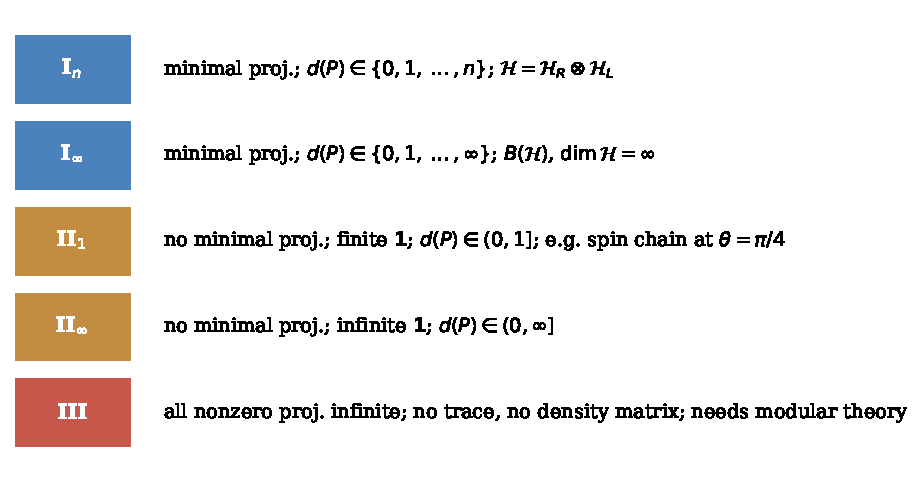
\includegraphics[width=0.88\textwidth]{figs/fig_type_chart.pdf}
\caption{The taxonomy of von Neumann algebra factors: classified by Murray and von Neumann according to the range of their projection dimension function $d(\mathcal{P}(\M))$ and the existence of a tracial state $\tau$. Type I possesses minimal projections (rank-one rays); Type II has no minimal projections but supports a trace (finite for $\mathrm{II}_1$, semifinite for $\mathrm{II}_\infty$); Type III has neither minimal projections nor a trace, exhibiting purely infinite projection dimensions.}
\label{fig:type_chart}
\end{figure}

\begin{table}[htbp]
\centering
\footnotesize
\begin{tabularx}{\textwidth}{@{}l p{2.2cm} l p{2.6cm} X l@{}}
\toprule
\textbf{Factor} & \textbf{Proj. Dim. $d(\mathcal{P})$} & \textbf{Trace $\tau$} & \textbf{Density Matrix $\rho_\M$} & \textbf{Physical System} & \textbf{Entropy Status} \\
\midrule
$\mathrm{I}_n$ & $\{0, 1, \dots, n\}$ & Yes (finite) & $\rho_R = \Tr_L\ket\Psi\bra\Psi$ & $n$-level system / qubits & $S \ge 0$ \\
$\mathrm{I}_\infty$ & $\{0, 1, 2, \dots, \infty\}$ & Yes (semifinite) & Fock space $\rho$ & Harmonic oscillator & Well-defined \\
$\mathrm{II}_1$ & $[0, 1]$ (continuous) & $\tau(\id)=1$ & $\rho_\M \in \M$ & $\infty$ Bell pairs ($\theta=\frac{\pi}{4}$) & $S \le 0$ (vs max-mixed) \\
$\mathrm{II}_\infty$ & $[0, \infty]$ (continuous) & Semifinite & $\rho_\M = e^{-K_\Psi - p}$ & Crossed product $\M \rtimes \mathbb{R}$ & $S_{\rm gen} = \frac{\langle\hat A\rangle}{4G_N} + S_{\rm bulk}$ \\
$\mathrm{III}_0$ & $\{0, \infty\}$ & None & No density matrix & Non-ergodic flows & Ill-defined \\
$\mathrm{III}_\lambda$ & $\{0, \infty\}$ & None & No density matrix & Spin chain ($\tan^2\theta = \lambda$) & Relative $S(\rho\|\sigma)$ only \\
$\mathrm{III}_1$ & $\{0, \infty\}$ & None & No density matrix & QFT subregion / Rindler & Relative only / crossed \\
\bottomrule
\end{tabularx}
\caption{Complete classification of von Neumann algebra factors and their physical, operational, and thermodynamic properties.}
\label{tab:factor_taxonomy}
\end{table}

\subsection{Sec.~III.A: density operators for type I and II algebras}

Here is the key new formula, and it deserves to be read as slowly as the definition of $\M$ itself was.
Suppose the full system is in a state $\ket\Psi\in\HH$, and $\M$ is a von Neumann algebra with a trace $\tr$
(so, by Sec.~II.C, type I or type II). Define $\rho_\M\in\M$ to be the operator satisfying
\[
\tr(A\rho_\M) = \braket{\Psi|A|\Psi} \qquad \text{for every } A\in\M
\]
(eq.~3.1). Positivity of $\tr$ guarantees this equation has a unique solution $\rho_\M$, and that the
resulting $\rho_\M$ is itself positive and correctly normalized — i.e., it genuinely deserves to be called a
density operator (footnote~18 of the paper flags a subtlety worth restating: it matters that $\rho_\M$ is
required to belong to $\M$ itself, not merely to $B(\HH)$ — the equation is being solved \emph{within} the
algebra). With $\rho_\M$ in hand, the entanglement entropy is defined exactly as you'd expect,
\[
S_\M \equiv -\tr(\rho_\M\log\rho_\M)
\]
(eq.~3.2) — formally identical to the ordinary formula $S_R=-\Tr(\rho_R\log\rho_R)$, just with $\tr$ (the
algebra's own, possibly renormalized trace from Sec.~II.C) standing in for the ordinary Hilbert-space trace,
and $\rho_\M$ standing in for the ordinary reduced density matrix.

Stop and compare this to the formula you already know, $\rho_R=\Tr_L\ket\Psi\!\bra\Psi$ (a partial trace).
That formula needs the complement $L$ to be given explicitly, as a separate tensor factor you can sum over —
you need to know about the part of the world you \emph{cannot} access in order to build an object describing
the part you \emph{can}. Equation~3.1 needs nothing of the sort: it's a self-contained equation stated purely
in terms of $\M$'s own trace and expectation values of $\M$'s own operators. This is worth stating as
explicitly as the paper does in its own remark: since you only have access to $\M$, in what sense does
$\rho_\M$, defined this way, capture anything about entanglement with the outside world at all? The paper's
own promise (repeated here, since it's the right way to hold the question while reading the rest of the
section): the answer depends entirely on which \emph{type} $\M$ turns out to be, and working through that
answer, type by type, is the entire content of the rest of Sec.~III and all of Sec.~IV.

\subsection{Sec.~III.B: type I algebras}

\subsubsection*{The type I factor case: nothing is lost}

When $\M$ is a type I \emph{factor}, Sec.~II.C already established $\HH=\HH_R\otimes\HH_L$,
$\M=B(\HH_R)\otimes\id_L$, $\tr=\Tr_{\HH_R}$, $\M'=\id_R\otimes B(\HH_L)$ (eq.~3.3). Plug this into the
right-hand side of eq.~3.1: using the ordinary partial-trace formula, $\braket{\Psi|A|\Psi}=\Tr_{\HH_R}(\rho_R
A)$ for $A\in\M$ (eq.~3.4), where $\rho_R=\Tr_{\HH_L}\ket\Psi\bra\Psi$ is the ordinary reduced density matrix
you already know. Comparing this to the defining equation of $\rho_\M$ (eq.~3.1), and using $\tr=\Tr_{\HH_R}$,
you read off immediately: $\rho_\M=\rho_R$. The new, algebra-intrinsic definition and the old,
partial-trace definition give \emph{exactly} the same operator, whenever a type I factorization is available.
Nothing is lost by switching definitions — you can check this is consistent rather than just asserted, since
both sides of eq.~3.1 are now completely explicit ordinary-linear-algebra objects.

Two remarks the paper makes here are worth keeping, because they're exactly the seeds of everything that
happens once type I stops being available:
\begin{enumerate}
\item The two approaches are conceptually very different, even when they agree numerically. Equation~2.2
needs the full global state $\ket\Psi$, including the part living in $\HH_L$ that you have no access to, in
order to build $\rho_R$. Equation~3.1 needs only expectation values of operators in $\M$ — data an
$R$-observer could, in principle, actually collect. The fact that these two completely different-looking
recipes produce the same answer, in the type I case, is itself the thing worth remembering when type I stops
holding: the entanglement information was, all along, fully recoverable from $\M$'s own internal data; the
tensor-product recipe was just a more roundabout way of getting the same answer, one that happens to break
once no factorization exists.
\item Because $\tr$ (equal here to the ordinary $\Tr_{\HH_R}$) genuinely counts basis states of an honest
Hilbert space $\HH_R$, $S_\M=S_R$ inherits a completely ordinary statistical interpretation — the usual
``number of effectively occupied states'' reading of entropy. This interpretation, too, is about to become
much more delicate once you leave type I.
\end{enumerate}

\subsubsection*{General type I: a nontrivial center, and where lattice gauge theory fits}

If $\M$ is type I but \emph{not} a factor (it has a nontrivial center — recall the block-diagonal
$P_1,P_2$ worked example from Sec.~II.B.2 of this companion), the Hilbert space decomposes into a direct sum
of sectors, one for each value $\alpha$ of the central (classical) label:
\[
\HH=\bigoplus_\alpha\HH_\alpha, \quad \HH_\alpha=\HH_{R\alpha}\otimes\HH_{L\alpha}, \qquad
\M=\bigoplus_\alpha\big(B(\HH_{R\alpha})\otimes\id_{L\alpha}\big)
\]
(eqs.~3.5--3.6) — within each sector, the ordinary tensor-product story holds exactly as in the factor case
above; the different sectors just sit side by side, never mixing (any operator in $\M$ acts block-diagonally,
never sending a state in sector $\alpha$ to a state in a different sector $\alpha'$). The trace is built
sector by sector, $\tr A=\sum_\alpha\Tr_{\HH_{R\alpha}}A_\alpha$ (eq.~3.7), and a general state $\rho$ on
$\HH$ decomposes as $\rho=\bigoplus_\alpha p_\alpha\rho_\alpha$ — a classical probability $p_\alpha$ of being
in sector $\alpha$, times an ordinary (normalized) density matrix $\rho_\alpha$ within that sector (eq.~3.8).
Working through eq.~3.1 sector by sector gives $\rho_\M=\bigoplus_\alpha p_\alpha(\rho_{R\alpha}\otimes
\id_{L\alpha})$ (eq.~3.9, with $\rho_{R\alpha}=\Tr_{\HH_{L\alpha}}\rho_\alpha$ the ordinary reduced density
matrix within sector $\alpha$), and plugging this into eq.~3.2 gives an entropy that cleanly splits into two
recognizable pieces,
\[
S_\M = -\sum_\alpha p_\alpha\log p_\alpha \;+\; \sum_\alpha p_\alpha S_\alpha ,
\qquad S_\alpha=-\tr_\alpha(\rho_{R\alpha}\log\rho_{R\alpha})
\]
(eq.~3.10): an ordinary classical (Shannon) entropy of \emph{which sector you're in}, plus the
probability-weighted average of the ordinary quantum entanglement entropy \emph{within} each sector. Nothing
here is conceptually new — it's exactly what you'd compute by hand if someone told you ``the system is either
in configuration A with probability $p_A$ (itself entangled some amount $S_A$) or configuration B with
probability $p_B$ (entangled some amount $S_B$), and you don't know which'' — but it's worth seeing it fall
directly out of the single unified formula, eq.~3.1, rather than needing to be reasoned out from scratch each
time.

\begin{quote}
\textit{Worked example: superselection sectors and entanglement in a 2-site lattice gauge model.} Consider a spatial lattice with two sites ($x_1, x_2$) connected by a gauge link carrying electric flux $E \in \{0, 1\}$. The physical Hilbert space decomposes into superselection sectors labeled by the central electric flux $q \in \{0, 1\}$ passing across the bipartition cut between the sites:
\[
\HH_{\text{phys}} = \HH_{q=0} \oplus \HH_{q=1} = (\HH_{R,0}\otimes\HH_{L,0}) \oplus (\HH_{R,1}\otimes\HH_{L,1}) .
\]
Suppose a physical state is prepared as a mixture of these sectors:
\[
\rho = p_0\,\rho_0 \oplus p_1\,\rho_1 , \qquad p_0 = 0.8, \quad p_1 = 0.2 ,
\]
where in sector $q=0$ the two sites are maximally entangled Bell pairs with reduced density matrix $\rho_{R,0} = \operatorname{diag}(1/2, 1/2)$ ($S_0 = \log 2 \approx 0.6931$), while in sector $q=1$ the sites are unentangled product states ($S_1 = 0$).
Evaluating the unified algebraic entropy formula (eq.~3.10):
\begin{enumerate}
\item \textbf{Classical Shannon entropy of the gauge flux:}
\[
H(p) = -p_0\log p_0 - p_1\log p_1 = -0.8\log(0.8) - 0.2\log(0.2) \approx 0.1785 + 0.3219 = 0.5004\text{ nats} .
\]
\item \textbf{Average quantum entanglement within sectors:}
\[
\sum_\alpha p_\alpha S_\alpha = 0.8 \times (\log 2) + 0.2 \times 0 = 0.8 \times 0.693147 = 0.5545\text{ nats} .
\]
\item \textbf{Total algebraic entropy:}
\[
S_\M = H(p) + \sum_\alpha p_\alpha S_\alpha \approx 0.5004 + 0.5545 = 1.0549\text{ nats} .
\]
\end{enumerate}
This demonstrates how the algebraic framework captures both classical gauge flux fluctuations and genuine quantum entanglement in a single formula without requiring a spatial tensor factorization.
\end{quote}

This is exactly the situation for the lattice gauge theory example (Ex.~1 from Sec.~I): the algebra of
gauge-invariant local operators is type I (it still has minimal projections, still counts states in the
ordinary way sector by sector) but not a factor (gauge invariance imposes a classical superselection label —
which gauge sector, e.g.\ which total electric flux configuration, you're in). The single formula~3.1 handles
this uniformly, with the factorized case (type I factor) simply being the special case of a trivial center
(only one sector, $p_\alpha=1$ for a single $\alpha$). This is the sense in which the algebraic language,
even at this early, still-mostly-familiar stage, is already doing real unifying work.

\subsection{Sec.~III.C: type II algebras}

This is where something genuinely new happens, and the paper's chosen way to show it is to build a type
$\mathrm{II}_1$ factor completely explicitly, by hand, out of the $N\to\infty$ Bell-pair chain from
Sec.~II.E of this companion. It's worth doing every step of this construction, because it is the first
place in the paper where you can watch an entirely new kind of mathematical object get built in front of you,
out of nothing more exotic than an infinite chain of ordinary qubits.

\subsubsection*{Sec.~III.C.1: building a trace at $\theta=\pi/4$}

Recall the setup from Sec.~II.E: $\M\equiv\M_R$ is the von Neumann algebra of operators acting on the
right-hand spins of the chain, built via GNS from the algebra of finite-energy operations $\Alg_R$ and the
state $\omega_\theta(A)=\braket{\Phi_\theta|A|\Phi_\theta}$. Fix $\theta=\pi/4$ (every pair maximally
entangled) and \emph{define}
\[
\tr A \equiv \braket{\Phi_{\pi/4}|A|\Phi_{\pi/4}} , \qquad A\in\M .
\]
(eq.~3.11.) This looks, on the surface, exactly like an ordinary expectation value — nothing distinguishes it
notationally from $\omega_{\pi/4}(A)$ already defined in Sec.~II.E. The claim being made is that, specifically
at $\theta=\pi/4$, this particular expectation value happens to \emph{also} satisfy the cyclic property
$\tr(AB)=\tr(BA)$ that defines a trace (Sec.~II.B.3) — and it's worth verifying this rather than just
believing it, since it is the single fact the entire rest of this subsection rests on.

\textbf{Step 1: a single pair.} Take one spin pair at $\theta=\pi/4$, in the state $\ket{\phi_{\pi/4}}=
\tfrac1{\sqrt2}(\ket{00}+\ket{11})$, and let $a = \begin{pmatrix} a_{00} & a_{01} \\ a_{10} & a_{11} \end{pmatrix}$ be any operator acting on the right spin alone ($a\otimes\id_L$). Let us compute the expectation value by expanding the state:
\begin{align*}
\braket{\phi_{\pi/4}|a\otimes\id_L|\phi_{\pi/4}} &= \frac{1}{2}\left(\bra{00}+\bra{11}\right)(a\otimes\id_L)\left(\ket{00}+\ket{11}\right) \\
&= \frac{1}{2}\left( \braket{00|a\otimes\id|00} + \braket{00|a\otimes\id|11} + \braket{11|a\otimes\id|00} + \braket{11|a\otimes\id|11} \right) \\
&= \frac{1}{2}\left( a_{00}\braket{0|0}_L + a_{01}\braket{0|1}_L + a_{10}\braket{1|0}_L + a_{11}\braket{1|1}_L \right) \\
&= \frac{1}{2}\left( a_{00} + a_{11} \right) = \frac{1}{2}\Tr_2(a) .
\end{align*}
(eq.~3.12, with $\Tr_2$ the ordinary $2\times2$ matrix trace) — the expectation value in a single maximally
entangled pair, of any operator touching only one side of that pair, is exactly one-half the ordinary trace
of that operator. This specific numerical coefficient, $\tfrac12$, is not an accident of notation; it's
exactly $1/\dim(\HH_2)$ for a single qubit, and it will reappear, tracked explicitly, in eq.~3.18 below.

\textbf{Step 2: many pairs.} A general element of $\M_R$ (recall Sec.~II.E, eq.~2.57) is $A=a_1\otimes
a_2\otimes\cdots$, with only finitely many of the $a_i$ different from the identity — say $a_{i_1},\dots,
a_{i_k}$ are the nontrivial ones. Because $\ket{\Phi_{\pi/4}}$ is a product of independent pairs, and each
pair contributes independently via Step~1,
\[
\braket{\Phi_{\pi/4}|A|\Phi_{\pi/4}} = \frac{1}{2^k}\,\Tr_2(a_{i_1})\cdots\Tr_2(a_{i_k})
\]
(eq.~3.13) — the expectation value in the full infinite chain reduces to a product of ordinary $2\times2$
matrix traces, one factor of $\tfrac12$ for each of the $k$ pairs actually touched.

\textbf{Step 3: cyclicity.} Here is the punchline, and it's genuinely just a one-line consequence of Step~2
once you see it: since $\braket{\Phi_{\pi/4}|A|\Phi_{\pi/4}}$ reduces \emph{entirely} to a product of ordinary
$2\times2$ matrix traces, and the ordinary matrix trace is itself cyclic ($\Tr_2(a_ib_i)=\Tr_2(b_ia_i)$ for
each individual pair, a completely standard fact about matrix traces), the whole product inherits cyclicity:
\[
\braket{\Phi_{\pi/4}|AB|\Phi_{\pi/4}} = \braket{\Phi_{\pi/4}|BA|\Phi_{\pi/4}}
\]
(eq.~3.14). This establishes eq.~3.11 as a genuine trace on $\M$. And this is exactly where $\theta=\pi/4$
earns its special status: Step~1's formula, $\braket{\phi_\theta|a|\phi_\theta}=\tfrac12\Tr_2(a)$, is only
exactly true at $\theta=\pi/4$ — for any other angle, the expectation value picks up $\theta$-dependent
weighting that breaks the exact matching to an ordinary matrix trace, and cyclicity fails. While this is often stated without derivation, we can prove the impossibility of any trace directly and rigorously via macroscopic operator condensation:

\begin{keyresult}[: The No-Trace Theorem for the Asymmetric Spin Chain]
\textbf{Theorem:} Let $\Alg_R = \bigotimes_{k=1}^\infty M_2(\mathbb{C})$ be the quasi-local spin chain algebra, and let $\ket{\Phi_\theta} = \bigotimes_{k=1}^\infty (\cos\theta\ket{00} + \sin\theta\ket{11})_k$ with $\theta \in (0, \pi/4)$. Let $\M_R \equiv \pi_\theta(\Alg_R)'' \subseteq B(\HH_\theta)$ be the GNS von Neumann factor.
Then for any $\theta \ne \pi/4$, \textbf{there exists no nonzero normal tracial state on $\M_R$}. Consequently, $\M_R$ is strictly type III.

\textbf{Proof:}
\begin{enumerate}[leftmargin=*]
\item \textbf{Tracial constraint on Pauli commutators:}
Suppose for contradiction that there exists a normal tracial state $\tau: \M_R \to \mathbb{C}$ with $\tau(\id) = 1$. By definition of a trace, $\tau(AB) = \tau(BA)$ for all $A, B \in \M_R$, which implies that $\tau([A, B]) = 0$ for every commutator.
On any individual spin site $k$, consider the Pauli operators $\sigma_x^{(k)}, \sigma_y^{(k)}, \sigma_z^{(k)} \in \Alg_R \subset \M_R$. From the $\mathfrak{su}(2)$ algebra, $[\sigma_x, \sigma_y] = 2i\sigma_z$, which gives:
\[
\sigma_z^{(k)} = \frac{1}{2i}\big[\sigma_x^{(k)}, \, \sigma_y^{(k)}\big] .
\]
Applying the tracial state $\tau$ directly yields:
\[
\tau\big(\sigma_z^{(k)}\big) = \frac{1}{2i}\tau\big([\sigma_x^{(k)}, \, \sigma_y^{(k)}]\big) = 0 \qquad \text{for all } k \ge 1 .
\]

\item \textbf{Vanishing trace of average magnetization:}
Define the macroscopic block-spin average magnetization over the first $N$ sites:
\[
M_N \equiv \frac{1}{N}\sum_{k=1}^N \sigma_z^{(k)} \in \M_R .
\]
By linearity of $\tau$ and the single-site identity above:
\[
\tau(M_N) = \frac{1}{N}\sum_{k=1}^N \tau\big(\sigma_z^{(k)}\big) = 0 \qquad \text{for all } N \ge 1 .
\]

\item \textbf{Macroscopic condensation in the GNS state:}
Now examine $M_N$ in the physical GNS reference state $\ket{\Omega_\theta} \equiv \ket{\Phi_\theta}$. On each entangled pair:
\[
\braket{\phi_\theta | \sigma_z | \phi_\theta} = \cos^2\theta \braket{0|\sigma_z|0} + \sin^2\theta \braket{1|\sigma_z|1} = \cos^2\theta - \sin^2\theta = \cos(2\theta) .
\]
The expectation value of the average magnetization is therefore:
\[
\braket{\Omega_\theta | M_N | \Omega_\theta} = \frac{1}{N}\sum_{k=1}^N \cos(2\theta) = \cos(2\theta) .
\]
Because the state $\ket{\Phi_\theta}$ is an exact product state across different pairs, spin fluctuations at distinct sites $k \ne j$ are completely uncorrelated:
\[
\Braket{\Omega_\theta \Big| \big(\sigma_z^{(k)} - \cos(2\theta)\big)\big(\sigma_z^{(j)} - \cos(2\theta)\big) \Big| \Omega_\theta} = \delta_{kj}\big(1 - \cos^2(2\theta)\big) = \delta_{kj}\sin^2(2\theta) .
\]
The variance of $M_N$ in the GNS representation is:
\[
\big\| \big(M_N - \cos(2\theta)\id\big)\ket{\Omega_\theta} \big\|^2 = \frac{1}{N^2}\sum_{k=1}^N \sin^2(2\theta) = \frac{\sin^2(2\theta)}{N} \xrightarrow{N\to\infty} 0 .
\]

\item \textbf{Strong operator convergence:}
Since $\ket{\Omega_\theta}$ is cyclic and separating for $\M_R$, and $\|M_N\| \le 1$ is uniformly bounded, the vanishing of the variance implies that $M_N$ converges in the strong operator topology on $\HH_\theta$ to a scalar multiple of the identity:
\[
\mathrm{s\text{-}}\lim_{N\to\infty} M_N = \cos(2\theta)\,\id .
\]

\item \textbf{The contradiction:}
By definition of normality, the state $\tau$ is continuous in the weak (and ultraweak) operator topology. Therefore:
\[
\lim_{N\to\infty} \tau(M_N) = \tau\big(\mathrm{s\text{-}}\lim_{N\to\infty} M_N\big) = \tau\big(\cos(2\theta)\id\big) = \cos(2\theta)\,\tau(\id) = \cos(2\theta) .
\]
Comparing this with the exact algebraic result from Step~2:
\[
0 = \lim_{N\to\infty} \tau(M_N) = \cos(2\theta) .
\]
For any non-maximal entangling angle $\theta \in (0, \pi/4)$, we have $\cos(2\theta) > 0$. The equality $0 = \cos(2\theta) > 0$ is a strict contradiction!

Hence no normal tracial state $\tau$ can exist on $\M_R$ when $\theta \ne \pi/4$. With both type I and type II ruled out by the total absence of a trace, $\M_R$ is unavoidably \textbf{type III}. $\blacksquare$
\end{enumerate}
\end{keyresult}

\subsubsection*{Sec.~III.C.2: no minimal projection, and dimensions that are genuine real numbers}

With a bona fide trace in hand, $\M_R$ (at $\theta=\pi/4$) is at least type I or type II — the question is
which. Consider the family of projections built by fixing some finite subset of the spins to be spin-up,
and leaving the rest untouched:
\[
\id \equiv \id_2\otimes\id_2\otimes\cdots, \qquad
P_1 = \id_2\otimes P_\uparrow\otimes\id_2\otimes\cdots, \qquad
P_2 = P_\uparrow\otimes\id_2\otimes P_\uparrow\otimes\id_2\otimes\cdots,
\]
with $P_\uparrow=\begin{psmallmatrix}1&0\\0&0\end{psmallmatrix}$ the projector onto spin-up on a single qubit
(eq.~3.16) — and, in general, you can build a projection this way by choosing \emph{any} finite subset of the
spins and replacing their identity factor with $P_\uparrow$.

Here is the argument that no minimal projection exists, and it's worth seeing why it's airtight rather than
just plausible: take \emph{any} nonzero projection $P$ of this form, built by fixing some finite set of spins.
No matter how many spins it already fixes, you can always find one more spin, currently left as $\id_2$
inside $P$, and replace that one factor with $P_\uparrow$ too — producing a new projection $\widetilde P$ that
is strictly smaller than $P$ (fixing one additional spin can only shrink the corresponding subspace, never
grow it) and still manifestly nonzero. Since this can be done starting from \emph{any} such $P$, with no
exception, there is no smallest one — no projection built this way can be minimal. So $\M_R$ has finite
projections (as you're about to see) but no minimal ones: by the Sec.~II.C classification, this rules out
type I entirely.

Now compute actual dimensions, using the trace normalized so $d(\id)=\tr(\id)=1$ (eq.~3.17 — automatic, since
$\tr(\id)=\braket{\Phi_{\pi/4}|\id|\Phi_{\pi/4}}=1$ by normalization of the state). Using Step~2's formula
above directly: $P_1$ fixes exactly one spin to $P_\uparrow$ (with $\Tr_2(P_\uparrow)=1$), so
$d(P_1)=\tr(P_1)=\tfrac12\Tr_2(P_\uparrow)=\tfrac12$; $P_2$ fixes two spins, so
$d(P_2)=\tr(P_2)=\tfrac1{2^2}\Tr_2(P_\uparrow)\Tr_2(P_\uparrow)=\tfrac14$ (eq.~3.18) — and in general, a
projection fixing $k$ spins has dimension exactly $2^{-k}$. Check this is completely consistent, not just
plausible: for any finite $k$, $2^{-k}>0$ (never actually zero, however large $k$ is), so every one of these
projections is genuinely nonzero and finite — consistent with there being no minimal one (you can always
halve the dimension again by fixing one more spin, but you never reach zero at any finite step).

This is the moment where something with literally no counterpart in ordinary finite-dimensional linear
algebra appears: by taking superpositions of orthogonal projections built this way (and limits of such
superpositions — infinite sums, made rigorous by the completeness built into the von Neumann algebra
structure), you can construct a projection $P$ with $d(P)$ equal to \emph{any} real number in $(0,1]$, not
just the numbers $2^{-k}$ reachable by the simple fixed-spin construction above. Compare this once more to
ordinary quantum mechanics: there, ``the dimension of a subspace'' is always a whole number, obtained by
literally counting basis vectors — there is no such thing as a subspace of dimension $0.31830989\ldots$ (an
arbitrary real number). Here, $d(P)$ genuinely can be any such number, and this continuous range of possible
dimensions, together with the complete absence of a minimal projection, is precisely the defining signature
of type $\mathrm{II}_1$ (Sec.~II.C): finite projections exist and can be directly compared in size, but there
is no smallest possible ``one unit'' of measurement, only an ever-refinable continuum. So: at $\theta=\pi/4$,
$\M=\M_R$ is a type $\mathrm{II}_1$ factor — the first genuinely new object encountered so far in this
companion, and it was built using nothing beyond ordinary spin-$\tfrac12$ qubits and an infinite chain of
them.

\begin{figure}[htbp]
\centering
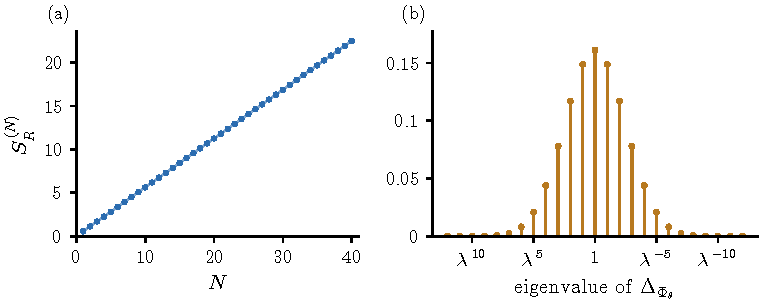
\includegraphics[width=0.78\textwidth]{figs/fig_spin_chain_typeIII.pdf}
\caption{The emergence of non-Type I factor structures from an infinite spin chain: as the number of entangled qubit pairs $N \to \infty$, the discrete eigenvalues of the reduced state merge into a continuous spectrum. At $\theta = \pi/4$, the algebra becomes the hyperfinite Type $\mathrm{II}_1$ factor where projections span a continuous dimension range $d(P) \in [0,1]$. For generic $\theta \in (0, \pi/4)$, the modular operator spectrum spans geometric powers $\lambda^k = (\tan^2\theta)^k$, forming a Type $\mathrm{III}_\lambda$ factor.}
\label{fig:spin_chain_typeIII}
\end{figure}

\subsubsection*{Interpreting $\rho_\M$ and $S_\M$: an entropy that can be negative}

With the type $\mathrm{II}_1$ trace of eq.~3.11 in hand, eq.~3.1 can be used to compute $\rho_\M$ and eq.~3.2
to compute $S_\M$ for any state you like — and the results have a genuinely surprising feature that's worth
working through with actual numbers, because it looks, at first glance, like it must be a mistake.

Take a state $\ket\Psi$ equal to $\ket{\Phi_{\pi/4}}$ everywhere except that a finite number $k$ of the pairs,
labelled $i_1,\dots,i_k$, are instead prepared in some other two-qubit state $\eta_{i_s}$ (eq.~3.19). Solving
eq.~3.1 for this state (a direct computation, using the same pair-by-pair factorization as Step~2 above) gives
\[
\rho_\M(\Psi) = 2\rho_1\otimes2\rho_2\otimes\cdots\otimes2\rho_n\otimes\cdots
\]
(eq.~3.20), where $\rho_i$ is the ordinary reduced density matrix of pair $i$ in the state $\eta_i$ (and
$2\rho_i=\id_2$ for every pair not among $i_1,\dots,i_k$ — the factor of $2$ coming directly from the
$\tfrac12$ in eq.~3.12). As a sanity check on the normalization: plugging in $\Psi=\Phi_{\pi/4}$ itself gives
$\rho_\M(\Phi_{\pi/4})=\id$ exactly (eq.~3.21) — the trace's own defining state is, unsurprisingly, assigned
the identity as its density operator, since $\tr(A\cdot\id)=\tr(A)=\braket{\Phi_{\pi/4}|A|\Phi_{\pi/4}}$ by
the very definition of $\tr$.

Plugging eq.~3.20 into the entropy formula, eq.~3.2, gives (eq.~3.22)
\[
S_\M(\Psi) = \sum_{s=1}^k S_2(\rho_{i_s}) - k\log2 ,
\]
where $S_2(\rho_{i_s})$ is the ordinary, ranges-from-$0$-to-$\log2$ entanglement entropy of the single
perturbed pair $i_s$. Here is a completely concrete instance, worked with an actual number: take $k=1$, and
let the one perturbed pair be prepared at angle $\phi=0.3$ radians instead of $\pi/4\approx0.785$ radians (so
$\eta_{i_1}=\cos(0.3)\ket{00}+\sin(0.3)\ket{11}$, a less-than-maximally-entangled pair). Direct computation
gives $S_2(\rho_{i_1})\approx0.2963$ (from $p_0=\cos^2(0.3)\approx0.9139$, $p_1=\sin^2(0.3)\approx0.0861$, and
the ordinary two-level entropy formula), while $\log2\approx0.6931$. So
\[
S_\M(\Psi) \approx 0.2963 - 0.6931 = -0.3968 ,
\]
a genuinely, checkably \emph{negative} number. And this isn't a fluke of the particular angle chosen: since
$S_2(\rho_{i_s})\le\log2$ always (the ordinary two-level entropy is bounded above by $\log2$, with equality
only at exact maximal entanglement), every term in the sum in eq.~3.22 satisfies $S_2(\rho_{i_s})-\log2\le0$,
so $S_\M(\Psi)\le0$ for \emph{every} state built this way, with equality only in the degenerate case where
every perturbed pair happens to still be exactly maximally entangled.

This looks alarming on first sight: $\rho_\M$ is a genuine, positive, correctly-normalized density operator
($\tr\rho_\M=1$, exactly the way a density operator should be), and yet $-\tr(\rho_\M\log\rho_\M)$ came out
negative — something that could \emph{never} happen for the entropy of an ordinary, finite-dimensional density
matrix (where $-\Tr(\rho\log\rho)\ge0$ always, with equality only for a pure state). There is no contradiction,
and the resolution is worth stating as plainly as possible: $\tr$ here is \emph{not} the ordinary matrix trace
that counts basis states one at a time. It was built, in Sec.~III.C.1 above, directly out of expectation
values in the maximally entangled reference state $\ket{\Phi_{\pi/4}}$ — and in a type II algebra there is no
minimal projection to serve as ``one state,'' so $\tr$ never had the ``count the dimensions'' interpretation
that makes the ordinary entropy formula manifestly non-negative in the first place.

What eq.~3.22 is actually computing, the paper shows directly, is minus a \emph{relative} entropy:
\[
S_\M(\Psi) = -S_\M(\Psi\,\|\,\Phi_{\pi/4})
\]
(this also follows, more generally and without needing the special simple form of eq.~3.19, directly from
eq.~3.24 in the paper) — the ordinary relative entropy $S(\rho\|\sigma)=\Tr\rho(\log\rho-\log\sigma)$ from
Sec.~I of this companion, applied here with $\rho=\rho_\M(\Psi)$ and $\sigma=\rho_\M(\Phi_{\pi/4})=\id$.
Relative entropy measures \emph{distinguishability from a chosen reference}, and there is nothing about its
definition that prevents $-S(\rho\|\sigma)$ from being negative — quite the opposite, $S(\rho\|\sigma)\ge0$
always, so $-S(\rho\|\sigma)\le0$ always, exactly matching what was just computed. The entropy $S_\M$ in a
type II algebra should be read not as ``how many microstates does this occupy,'' the ordinary statistical
reading that only makes sense once there's a minimal projection to count from, but as \textbf{a signed
distance from the maximally entangled background state that defines the trace in the first place} — a
\emph{relative}, not absolute, quantity, and this is the first concrete place in the paper where relative
entropy, rather than entropy on its own, reveals itself as the more fundamental and more robust object. It
survives, essentially unchanged in its definition, all the way through type III (Sec.~IV) and into the
holographic applications starting in Sec.~VI — ordinary entropy, as you've just seen directly, does not
survive intact even this far.

\begin{physconnect}[: Negative Relative Entropy in Qubits]
Before trusting that a genuinely negative ``entropy'' is a sensible thing for a serious theory to produce, it's
worth noticing that ordinary, finite-dimensional quantum mechanics already contains this phenomenon, in
disguise, using nothing beyond the relative entropy formula from Sec.~I. For an ordinary $d$-dimensional
quantum system, take the relative entropy of any state $\rho$ against the maximally mixed reference
$\sigma=\id/d$:
\[
S(\rho\|\sigma) = \Tr\rho\big(\log\rho - \log(\id/d)\big) = -S(\rho) + \log d ,
\]
using $S(\rho)\equiv-\Tr(\rho\log\rho)$ for the ordinary von Neumann entropy. Since $S(\rho)\le\log d$ always
(entropy never exceeds the maximally mixed value — a completely standard fact), $S(\rho\|\sigma)\ge0$, exactly
as relative entropy must be. Now just \emph{flip the sign} and look at $-S(\rho\|\sigma)=S(\rho)-\log d$. For
a qubit ($d=2$) in the state $\rho=\mathrm{diag}(0.9,0.1)$: $S(\rho)\approx0.325$, while $\log2\approx0.693$,
so $-S(\rho\|\sigma)\approx-0.368$ — \textbf{a manifestly negative number, computed from nothing more exotic
than an ordinary qubit's entropy, minus a constant.}

This is not a coincidence dressed up to look relevant — it is exactly the mechanism at work in
eq.~3.22 above, just with the additive constant made completely explicit. $S_\M$ in a type II algebra is
built the same way: an ordinary-looking entropy, measured relative to (i.e., shifted down by) whatever
baseline the maximally entangled reference state assigns. In finite dimensions that baseline is the familiar,
finite number $\log d$; in the type $\mathrm{II}_1$ Bell-pair-chain algebra, the same baseline is still there,
it's just been absorbed into the very definition of $\tr$ (built, recall, directly from the maximally entangled
$\ket{\Phi_{\pi/4}}$) rather than written as a separate $\log d$ term you subtract by hand. \textbf{Nothing
about the arithmetic of entropy changed} — subtracting a constant from an ordinary, everyday entropy was
always capable of giving a negative number. What's new in the type II case is only that the algebra itself,
having no minimal projection, leaves no alternative baseline (no ``$d$'') to normalize against — the maximally
entangled reference state is not a choice, it's the \emph{only} thing available to define $\tr$ with in the
first place.
\end{physconnect}

(One further bookkeeping note, briefly: the paper also observes that for a type $\mathrm{II}_\infty$ factor,
the same interpretation of $\rho_\M$ and $S_\M$ carries over, except that there is no preferred, canonical way
to normalize the trace — unlike the $\mathrm{II}_1$ case, where normalizing $d(\id)=1$ was a natural, forced
choice — so the entropy is only meaningfully defined up to an overall additive, state-independent constant.)

\subsection{Sec.~III.D: summary}

Pulling the type I and type II discussions together into one statement, worth having explicitly in view before
Sec.~IV introduces type III: the \emph{type} of the algebra $\M$ describing a subsystem determines, in a
completely general, state-independent way, what \emph{kind} of entanglement pattern every state of the full
system is forced into.

\begin{itemize}
\item \textbf{Type I factor.} A genuine tensor factorization exists. Pure, completely unentangled product
states exist inside the Hilbert space, and every state is either one of these or a superposition/mixture
built from them — exactly the ordinary Griffiths/Sakurai picture, recovered as the special case where nothing
new is happening.
\item \textbf{Type II factor.} No minimal projections exist, which means (a fact quoted here, following
directly from the definitions of Sec.~II.C: no minimal projection $\Rightarrow$ no pure state of $\M$ exists
at all) there is no unentangled reference state anywhere in sight. \emph{Every} state of the full system is
entangled across $(\M,\M')$ to some degree — there is no ``ground floor'' of zero entanglement to compare
against, only a maximally entangled reference state (the one that happens to define the trace), relative to
which the signed entropy of eq.~3.2 is measured.
\end{itemize}

Type III — where not even a trace exists, so eqs.~3.1 and 3.2 cannot be written down at all — is the subject
of the whole next section, and it is, as flagged repeatedly already, not an exotic corner case: it is the
type that actually governs local regions of relativistic quantum field theory, and holographic boundary
subalgebras in the strict large-$N$ limit that this paper's title promises to explain.

\section{Sec.~IV: Von Neumann algebras and entanglement: type III}

This is the technical heart of the whole paper, and it earns that description honestly: type III algebras have
no trace, so eqs.~3.1--3.2 (the density operator $\rho_\M$ and the entropy $S_\M$) simply cannot be written
down — there is no equation left to solve. And yet, as flagged repeatedly, type III is not some exotic
mathematical curiosity to be handled as a special case; it is the type that governs local regions of a
relativistic quantum field theory, and (as Sec.~VII will show) the type that governs holographic boundary
algebras in the strict large-$N$ limit. If the goal is to say anything at all about entanglement in exactly
the settings this paper cares about most, an entirely different tool is needed. That tool is
\textbf{Tomita--Takesaki modular theory}, and the core physical idea behind it is worth stating in one sentence
before any formalism: \emph{when a subsystem is highly entangled with its complement, not knowing about the
complement makes the subsystem look thermal} — entanglement, viewed from inside just one half, always looks
like heat. Everything in this section is that one idea, made completely precise.

\subsection{Sec.~IV.A: emergent times from entanglement — modular flows}

\subsubsection*{Starting from something you already understand: the type I case, retold}

To motivate the general construction, go back to an ordinary type I bipartite pure state $\ket\Psi$ with
full-rank reduced density matrix $\rho_R$ (``full-rank'' meaning invertible — every eigenvalue strictly
positive, so $\rho_R^{-1}$ exists; this will matter in a moment). Instead of studying the entropy $S_R$
directly, package the same information differently: write
\[
\rho_R = e^{-K_R}, \qquad K_R\equiv-\log\rho_R
\]
(eq.~4.1). $K_R$ is called the \textbf{entanglement Hamiltonian}, and $K_R\ge0$ (since $\rho_R$'s eigenvalues
are all in $(0,1]$, their negative logarithms are all $\ge0$). The full set of eigenvalues of $K_R$ — the
\emph{entanglement spectrum} — carries strictly more information than the entropy $S_R$ alone or any finite
list of R\'enyi entropies (each of those is just some specific weighted sum over the spectrum; the full
spectrum is the un-summed data), which is why condensed-matter physicists studying entanglement spectra
directly (rather than just the single number $S_R$) have found it such a fruitful diagnostic tool.

Now use $K_R$ to generate a flow:
\[
A(s) = e^{iK_Rs}Ae^{-iK_Rs} \in B(\HH_R), \qquad A\in B(\HH_R)
\]
(eq.~4.2) — this is formally identical to ordinary Heisenberg time evolution, $A(t)=e^{iHt}Ae^{-iHt}$, with
$K_R$ playing the role of a Hamiltonian and $s$ playing the role of time. It's called \textbf{modular flow},
and $s$ is called \textbf{modular time}. The key physical claim, which is really just the statement that
$e^{-K_R}=\rho_R$ is already, by construction, an ordinary Gibbs thermal density matrix at (dimensionless)
inverse temperature $\beta=1$ for the ``Hamiltonian'' $K_R$: an observer confined to $R$, using $s$ as their
notion of time, should see their system in thermal equilibrium — meaning correlation functions of
modular-flowed operators satisfy the \textbf{Kubo--Martin--Schwinger (KMS) condition}, the mathematical
signature of thermal equilibrium (spelled out precisely below).

You can do the same construction on the $L$ side, with $K_L=-\log\rho_L$. To treat both sides on equal
footing at once, define
\[
\Delta_\Psi \equiv \rho_R\otimes\rho_L^{-1}, \qquad -\log\Delta_\Psi = K_R - K_L
\]
(eq.~4.3), and let the modular flow act on operators of \emph{either} side:
\[
\sigma_s(A) \equiv \Delta_\Psi^{-is}A\Delta_\Psi^{is}\in B(\HH_R),\ \ A\in B(\HH_R), \qquad
\sigma_s(A') \equiv \Delta_\Psi^{-is}A'\Delta_\Psi^{is}\in B(\HH_L),\ \ A'\in B(\HH_L)
\]
(eqs.~4.4--4.5) — check this reduces to eq.~4.2 for $A\in B(\HH_R)$: since $\rho_L^{-1}$ (and hence any power
of it) commutes past $A\otimes\id_L$ trivially, $\Delta_\Psi^{-is}A\Delta_\Psi^{is}=\rho_R^{-is}A\rho_R^{is}$,
exactly eq.~4.2 with $s\leftrightarrow$ what was called $s$ there (a short but worthwhile check — it confirms
the joint object $\Delta_\Psi$ correctly reduces to the separate one-sided flows on each side). $\Delta_\Psi$
is called the \textbf{modular operator}.

\begin{quote}
\textit{Worked example, with actual numbers.} Take $\ket{\phi_\theta}=\cos\theta\ket{00}+\sin\theta\ket{11}$
from Sec.~I, so $\rho_R=\rho_L=\mathrm{diag}(\cos^2\theta,\sin^2\theta)$, and write out $\Delta_\Psi=
\rho_R\otimes\rho_L^{-1}$ as an explicit $4\times4$ matrix in the basis $\ket{00},\ket{01},\ket{10},\ket{11}$:
\[
\Delta_\Psi = \begin{pmatrix} 1&0&0&0\\ 0&\cos^2\theta/\sin^2\theta&0&0\\
0&0&\sin^2\theta/\cos^2\theta&0\\0&0&0&1\end{pmatrix} = \operatorname{diag}\left(1, \; \cot^2\theta, \; \tan^2\theta, \; 1\right) .
\]
Its eigenvalues are $1$ (multiplicity two, on $\ket{00}$ and $\ket{11}$), $\lambda\equiv\tan^2\theta$ (on $\ket{10}$), and $\lambda^{-1}=\cot^2\theta$ (on $\ket{01}$).

Now let us construct the Tomita operator $S_\Psi$, its adjoint $F_\Psi = S_\Psi^\dagger$, and the modular conjugation $J_\Psi$ explicitly from first principles:
\begin{enumerate}
\item \textbf{Action of the algebra on $\ket{\phi_\theta}$:} Any operator $A \in B(\HH_R)$ has the form $A = \begin{pmatrix} a & b \\ c & d \end{pmatrix}$. Its action on $\ket{\phi_\theta}$ produces:
\[
(A\otimes\id_L)\ket{\phi_\theta} = a\cos\theta\ket{00} + b\sin\theta\ket{01} + c\cos\theta\ket{10} + d\sin\theta\ket{11} .
\]
Given an arbitrary 4-component vector $\ket x = x_{00}\ket{00} + x_{01}\ket{01} + x_{10}\ket{10} + x_{11}\ket{11}$, matching coefficients gives $a = x_{00}/\cos\theta$, $b = x_{01}/\sin\theta$, $c = x_{10}/\cos\theta$, $d = x_{11}/\sin\theta$.

\item \textbf{The Tomita operator $S_\Psi$:} By definition, $S_\Psi$ maps $(A\otimes\id_L)\ket{\phi_\theta} \mapsto (A^\dagger\otimes\id_L)\ket{\phi_\theta}$. Since $A^\dagger = \begin{pmatrix} a^* & c^* \\ b^* & d^* \end{pmatrix}$, we have:
\[
(A^\dagger\otimes\id_L)\ket{\phi_\theta} = a^*\cos\theta\ket{00} + c^*\sin\theta\ket{01} + b^*\cos\theta\ket{10} + d^*\sin\theta\ket{11} .
\]
Substituting the expressions for $a,b,c,d$ in terms of $x_{ij}$:
\[
S_\Psi \begin{pmatrix} x_{00} \\ x_{01} \\ x_{10} \\ x_{11} \end{pmatrix} = \begin{pmatrix} x_{00}^* \\ \frac{\sin\theta}{\cos\theta} x_{10}^* \\ \frac{\cos\theta}{\sin\theta} x_{01}^* \\ x_{11}^* \end{pmatrix} = \begin{pmatrix} x_{00}^* \\ \tan\theta\, x_{10}^* \\ \cot\theta\, x_{01}^* \\ x_{11}^* \end{pmatrix} .
\]
Notice that applying $S_\Psi$ twice gives $S_\Psi^2\ket x = \ket x$, verifying $S_\Psi^2 = \id_4$ and $S_\Psi\ket{\phi_\theta} = \ket{\phi_\theta}$!

\item \textbf{The adjoint operator $F_\Psi \equiv S_\Psi^\dagger$:} From the inner product relation $\braket{y|S_\Psi x} = \braket{x|F_\Psi y}^*$, we find:
\[
F_\Psi \begin{pmatrix} y_{00} \\ y_{01} \\ y_{10} \\ y_{11} \end{pmatrix} = \begin{pmatrix} y_{00}^* \\ \cot\theta\, y_{10}^* \\ \tan\theta\, y_{01}^* \\ y_{11}^* \end{pmatrix} .
\]

\item \textbf{The modular operator $\Delta_\Psi = F_\Psi S_\Psi$:} Multiplying the two operators:
\[
\Delta_\Psi \begin{pmatrix} x_{00} \\ x_{01} \\ x_{10} \\ x_{11} \end{pmatrix} = F_\Psi \begin{pmatrix} x_{00}^* \\ \tan\theta\, x_{10}^* \\ \cot\theta\, x_{01}^* \\ x_{11}^* \end{pmatrix} = \begin{pmatrix} x_{00} \\ \cot^2\theta\, x_{01} \\ \tan^2\theta\, x_{10} \\ x_{11} \end{pmatrix} ,
\]
which is exactly the diagonal matrix $\Delta_\Psi = \operatorname{diag}(1, \cot^2\theta, \tan^2\theta, 1)$!

\item \textbf{The modular conjugation $J_\Psi = S_\Psi \Delta_\Psi^{-1/2}$:} The square root is $\Delta_\Psi^{1/2} = \operatorname{diag}(1, \cot\theta, \tan\theta, 1)$. Applying $S_\Psi$ to $\Delta_\Psi^{-1/2}\ket x$:
\[
J_\Psi \begin{pmatrix} x_{00} \\ x_{01} \\ x_{10} \\ x_{11} \end{pmatrix} = S_\Psi \begin{pmatrix} x_{00} \\ \tan\theta\, x_{01} \\ \cot\theta\, x_{10} \\ x_{11} \end{pmatrix} = \begin{pmatrix} x_{00}^* \\ x_{10}^* \\ x_{01}^* \\ x_{11}^* \end{pmatrix} .
\]
$J_\Psi$ is anti-unitary, satisfies $J_\Psi^2 = \id$, and acts as complex conjugation composed with the SWAP of qubits $\ket{01} \leftrightarrow \ket{10}$! Furthermore, $J_\Psi \Delta_\Psi J_\Psi = \Delta_\Psi^{-1}$.

\item \textbf{Exact modular flow on Pauli matrices:} The modular flow of an observable $A \in B(\HH_R)$ is $\sigma_s(A) = \Delta_\Psi^{-is} (A\otimes\id_L) \Delta_\Psi^{is}$.
\begin{itemize}
\item For $A = \sigma_z = \begin{pmatrix} 1 & 0 \\ 0 & -1 \end{pmatrix}$: since $\sigma_z \otimes \id_L = \operatorname{diag}(1, 1, -1, -1)$ commutes with $\Delta_\Psi$,
\[
\sigma_s(\sigma_z) = \sigma_z .
\]
\item For the raising operator $\sigma_+ = \begin{pmatrix} 0 & 1 \\ 0 & 0 \end{pmatrix}$: $\sigma_+ \otimes \id_L = \ket{00}\bra{10} + \ket{01}\bra{11}$. Evaluating:
\[
\sigma_s(\sigma_+) = \Delta_\Psi^{-is} (\sigma_+\otimes\id_L) \Delta_\Psi^{is} = (\tan^2\theta)^{is} \sigma_+ = e^{2is\log\tan\theta} \sigma_+ .
\]
Similarly, $\sigma_s(\sigma_-) = e^{-2is\log\tan\theta} \sigma_-$.
\item Since $\sigma_x = \sigma_+ + \sigma_-$ and $\sigma_y = -i(\sigma_+ - \sigma_-)$, we obtain:
\begin{align*}
\sigma_s(\sigma_x) &= \cos(2s\log\tan\theta)\,\sigma_x - \sin(2s\log\tan\theta)\,\sigma_y , \\
\sigma_s(\sigma_y) &= \cos(2s\log\tan\theta)\,\sigma_y + \sin(2s\log\tan\theta)\,\sigma_x .
\end{align*}
\end{itemize}
Modular flow on the qubit is an \textbf{exact spatial rotation} in the $xy$-plane of the Bloch sphere around the $z$-axis with constant angular frequency $\Omega = 2\log\cot\theta$!
\end{enumerate}
\end{quote}

Two facts about $\Delta_\Psi$ deserve to be stated plainly, because they are the two facts that survive,
completely unchanged in spirit, all the way to the fully general (type III) theory below.

\begin{enumerate}
\item $\Delta_\Psi\ket\Psi=\ket\Psi$, and in fact $\Delta_\Psi^{-1}\ket\Psi=\ket\Psi$ too, i.e.\
$(K_R-K_L)\ket\Psi=0$ (eq.~4.6) — check this directly on the worked example: $\ket\Psi=\ket{\phi_\theta}=
\cos\theta\ket{00}+\sin\theta\ket{11}$ is built entirely out of the two eigenvalue-$1$ eigenvectors of
$\Delta_\Psi$, so of course $\Delta_\Psi$ fixes it exactly. This says the modular flow is a kind of emergent,
purely internal time evolution under which the physical state itself never changes at all, even though the
flow acts nontrivially on operators living separately in $R$ and in $L$. This is also the precise, operator
version of the elementary fact that $S_R=S_L$ for a pure global state (Sec.~I): $\rho_R$ and $\rho_L$ have
the same set of eigenvalues (this is exactly what the Schmidt decomposition guarantees), so $K_R$ and $K_L$
have the same spectrum too, and $(K_R-K_L)\ket\Psi=0$ is one precise way of encoding that symmetry as an
operator statement.
\item Correlators of modular-flowed operators satisfy the KMS condition — made fully precise just below —
which is exactly the mathematical signature of thermal equilibrium at $\beta=1$: an observer with access only
to $R$ (or only to $L$), using modular time as their clock, experiences a genuinely thermal state.
\end{enumerate}

\subsubsection*{The swap operator $J_\Psi$}

There's a third, related object worth building explicitly, because it will reappear repeatedly. The
requirement that $\rho_R,\rho_L$ both be full-rank forces $\dim\HH_R=\dim\HH_L$ (a full-rank density matrix on
$\HH_R$ has as many nonzero eigenvalues as $\dim\HH_R$; by the Schmidt decomposition, that must match the
number of nonzero Schmidt coefficients, which is at most $\dim\HH_L$ too — so the two dimensions must agree
exactly for both reduced density matrices to be simultaneously full-rank). This matching dimension lets you
build an explicit \textbf{swap operator}: writing the Schmidt decomposition $\ket\Psi=\sum_n\sqrt{\lambda_n}
\ket n_R\ket n_L$, and a general vector $\ket\phi=\sum_{mn}\phi_{mn}\ket m_R\ket n_L$ in this same Schmidt
basis, define
\[
J_\Psi\ket\phi = \sum_{m,n}\phi_{mn}^*\ket n_R\ket m_L
\]
(eq.~4.7) — it swaps the labels $R\leftrightarrow L$ \emph{and} complex-conjugates every coefficient. $J_\Psi$
is \textbf{anti-unitary} (it involves that complex conjugation — a genuinely different kind of map from an
ordinary unitary, which is why it needs its own name), and $J_\Psi^2=\id$ (eq.~4.8, checked immediately: swap
twice and conjugate twice, and you're back where you started). One can check directly that conjugating an
operator in $\M=B(\HH_R)\otimes\id_L$ by $J_\Psi$ produces an operator in $\M'=\id_R\otimes B(\HH_L)$ — $J_\Psi$
literally exchanges the subsystem with its complement, at the level of operators, not just of vectors. This is
called the \textbf{modular conjugation operator}.

\subsubsection*{The key limitation, and the reformulation that removes it}

Everything above required $\rho_R,\rho_L$ full-rank — a real restriction, forcing (among other things)
$\dim\HH_R=\dim\HH_L$, which already rules out plenty of ordinary type I examples, let alone type II or III
where there's no $\rho_R$ at all. The entire strategic move of this subsection is to find a way of restating
``$\rho_R,\rho_L$ full-rank'' that makes no reference whatsoever to $\rho_R,\rho_L$ — so that it can survive
into a setting where those objects don't exist.

The needed restatement uses exactly the two properties singled out at the end of Sec.~II.D of this companion:
\textbf{cyclic} and \textbf{separating}. Recall: $\ket\Psi$ is cyclic with respect to $\M$ if $\{A\ket\Psi :
A\in\M\}$ is dense in $\HH$ (the algebra can reach essentially everywhere, starting from $\ket\Psi$); it is
separating with respect to $\M$ if $A\ket\Psi=0$ forces $A=0$ (no nonzero operator in $\M$ is wasted on
$\ket\Psi$). It's a short exercise (not carried out in the paper, but genuinely short) to check that
``$\rho_R,\rho_L$ both full-rank'' is \emph{exactly equivalent} to ``$\ket\Psi$ is cyclic with respect to both
$\M=B(\HH_R)\otimes\id_L$ and its commutant $\M'=\id_R\otimes B(\HH_L)$.'' And there's a further, genuinely
elegant simplification available: $\ket\Psi$ being cyclic with respect to $\M'$ turns out to be equivalent to
$\ket\Psi$ being \emph{separating} with respect to $\M$ (cyclic for the complement $\iff$ separating for the
algebra itself — a duality worth sitting with, since it means you never need to check both algebras
separately). So the entire condition collapses to a single, self-contained statement about $\M$ alone:
\textbf{$\ket\Psi$ is cyclic and separating with respect to $\M$.} This is a genuinely important moment in the
logical structure of the paper — it shows, one more time, that everything about bipartite entanglement really
is encoded in the algebra of just one side, with no need to reference the complement at all.

\subsubsection*{The Tomita--Takesaki theorem, stated in full}

Here is the theorem, and it holds for \emph{any} von Neumann algebra $\M$ with a cyclic and separating vector
$\ket\Psi$ — no reference anywhere in its statement to a trace, a density matrix, or a tensor factorization.
This is exactly why it survives into type III.

\begin{enumerate}
\item There is a positive operator $\Delta_\Psi$ (still called the \emph{modular operator}) leaving
$\ket\Psi$ invariant, $\Delta_\Psi\ket\Psi=\ket\Psi$ (eq.~4.9), and $K_\Psi\equiv-\log\Delta_\Psi$ generates a
genuine automorphism of $\M$ (a map from $\M$ to itself that respects all the algebra structure) and,
separately, of $\M'$:
\[
\sigma_s(A) \equiv \Delta_\Psi^{-is}A\Delta_\Psi^{is}\in\M\ \ \forall A\in\M,
\qquad
\sigma_s(A') \equiv \Delta_\Psi^{-is}A'\Delta_\Psi^{is}\in\M'\ \ \forall A'\in\M'
\]
(eqs.~4.10--4.11) — the flow really does stay inside the algebra it started in, at every modular time $s$, for
both $\M$ and $\M'$ separately.
\item There is an antiunitary \textbf{modular conjugation} $J_\Psi$ satisfying
$J_\Psi\ket\Psi=\ket\Psi$, $J_\Psi=J_\Psi^{-1}=J_\Psi^\dagger$, $J_\Psi\Delta_\Psi J_\Psi=\Delta_\Psi^{-1}$
(eq.~4.12), and $J_\Psi\M J_\Psi=\M'$, $J_\Psi\M'J_\Psi=\M$ (eq.~4.13) — $J_\Psi$ swaps $\M$ and $\M'$,
exactly the role the explicit swap operator played in the type I worked example above, now established as a
general fact.
\item A technical but important analyticity statement (eq.~4.14--4.15, stated here for completeness but not
needed for the physical content that follows): the vector $\Delta_\Psi^{-is}A\ket\Psi$, as a function of $s$,
extends to complex values of $s$ in the strip $\Im s\in(0,\tfrac12)$, with a specific relation,
$\Delta_\Psi^{-i(t+i/2)}A\ket\Psi=\Delta_\Psi^{-it}J_\Psi A^\dagger\ket\Psi$, holding on the boundary of that
strip.
\item Correlation functions of modular-flowed operators, $f_{AB}(s)\equiv\braket{\Psi|\sigma_s(A)B|\Psi}$,
analytically continue into the wider strip $\Im s\in(-1,0)$ and satisfy the \textbf{KMS relation}
\[
f_{AB}(s) = f_{BA}(-s-i)
\]
(eqs.~4.16--4.17) — this is the precise mathematical statement of ``looks thermal at $\beta=1$'': it is
exactly the periodicity-in-imaginary-time relation that an ordinary thermal correlator, $\Tr(e^{-\beta H}A(t)B)$,
satisfies (with $\beta=1$ here, and the KMS relation being the operator-algebra way of encoding the cyclic
property of the trace $\Tr(e^{-\beta H}\cdots)$ without ever needing $e^{-\beta H}$ to literally exist as a
trace-class operator — precisely what's needed once no trace exists at all, as in type III).
\end{enumerate}

\begin{physconnect}[: KMS Condition in Thermal QFT]
You have almost certainly already met the KMS relation, just not by that name, in an ordinary
finite-temperature quantum mechanics or statistical field theory course, and it's worth checking the
identical relation on a completely mundane example before trusting it applies to a type III algebra with no
Hamiltonian at all. Take an ordinary two-level system, $H=\omega\ket1\!\bra1 = \begin{pmatrix} 0 & 0 \\ 0 & \omega \end{pmatrix}$, in the thermal (Gibbs) state:
\[
\rho = \frac{e^{-\beta H}}{Z} = \frac{1}{1 + e^{-\beta\omega}} \begin{pmatrix} 1 & 0 \\ 0 & e^{-\beta\omega} \end{pmatrix} .
\]
For two operators $A, B$, define $f_{AB}(t) \equiv \Tr(\rho A(t) B)$ where $A(t) = e^{iHt} A e^{-iHt}$. Let us prove analytically that $f_{AB}(t) = f_{BA}(-t-i\beta)$:
\begin{align*}
f_{AB}(t) &= \Tr\left( \frac{e^{-\beta H}}{Z} e^{iHt} A e^{-iHt} B \right) \\
&= \Tr\left( B \, \frac{e^{-\beta H}}{Z} e^{iHt} A e^{-iHt} \right) \qquad \text{(by cyclicity of the trace)} \\
&= \Tr\left( \frac{e^{-\beta H}}{Z} \left[ e^{\beta H} B e^{-\beta H} \right] e^{iHt} A e^{-iHt} \right) \\
&= \Tr\left( \rho \, B(-i\beta) \, A(t) \right) .
\end{align*}
Applying time-translation invariance to both operators (shifting $t \to 0$ and $0 \to -t$):
\begin{align*}
f_{AB}(t) &= \Tr\left( \rho \, e^{-iHt} B(-i\beta) e^{iHt} \, A \right) = \Tr\left( \rho \, B(-t - i\beta) \, A \right) = f_{BA}(-t - i\beta) .
\end{align*}
This algebraic proof relies only on the cyclicity of the trace and the group property $e^{-\beta H} e^{iHt} = e^{i(t + i\beta)H}$. It shows why thermal states are periodic in imaginary time with period $\beta$. Tomita--Takesaki theory abstracts this exact property to define thermal states at $\beta=1$ without assuming a trace or Hamiltonian.

So what changed, going from this ordinary example to the general Tomita--Takesaki statement? Only this: here,
the flow generating $A(t)$ was an honest Hamiltonian $H$, and $\rho$ was a genuine, normalizable density
matrix you could write down as a finite matrix. In Sec.~IV.A's general theorem, neither of those needs to
exist — $\sigma_s$ can be \emph{some} flow with no Hamiltonian living in $\M$ at all (exactly the defining
property of type III, eq.~4.21), and there may be no $\rho$ to build a trace out of. The KMS relation survives
this demotion completely intact, because it was never really a statement about $H$ or $\rho$ individually —
it's a statement about the correlator $f_{AB}$ alone, which is exactly why it, rather than the Hamiltonian or
the density matrix, is the object General Tomita--Takesaki theory promotes to primary status.
\end{physconnect}

Read physically, in one sentence: \emph{any} operator algebra equipped with a cyclic-and-separating reference
vector automatically comes with a canonical, built-in notion of time flow, one under which the reference state
itself looks exactly thermal at inverse temperature $1$ — and this holds completely independently of whether
$\M$ has a trace. This is the sense in which the type I story above is not being generalized by analogy, but
literally subsumed as the special case where the canonical flow happens to be generated by an honest
Hamiltonian $K_R$ that lives inside $\M$ itself.

A handful of remarks the paper makes here are worth keeping explicitly:
\begin{itemize}
\item[(a)] Physically: given $\M$ and a cyclic-separating $\ket\Psi$, there is an emergent time evolution,
internal to $\M$ (or to $\M'$), that leaves $\ket\Psi$ fixed, and relative to which an observer confined to
$\M$ (or to $\M'$) feels a genuine temperature $1/\beta=1$.
\item[(b)] For type I, the cyclic-and-separating condition was a genuinely restrictive requirement (forcing
$\dim\HH_R=\dim\HH_L$). For the type III situations this paper actually cares about — quantum field theory,
statistical mechanics in the thermodynamic limit — this condition turns out to be satisfied \emph{generically},
as you'll see explicitly in Secs.~IV.C and IV.D below (Reeh--Schlieder theorem, and the $N\to\infty$
entangled-spin construction).
\item[(c)] The theorem is usually \emph{proved} (not merely stated) by first defining an antilinear
\textbf{Tomita operator} $S_\Psi$ directly from $\M$ and $\ket\Psi$,
\[
S_\Psi A\ket\Psi = A^\dagger\ket\Psi\ \ (A\in\M), \qquad
S_\Psi A'\ket\Psi = A'^\dagger\ket\Psi\ \ (A'\in\M') ,
\]
\[
S_\Psi^2=\id, \qquad S_\Psi\ket\Psi=\ket\Psi ,
\]
(eqs.~4.18--4.19 — note $S_\Psi$ is well-defined here precisely because $\ket\Psi$ is separating, the same
role separating played in the GNS construction of Sec.~II.D), and then taking its \textbf{polar
decomposition}: writing $S_\Psi=J_\Psi\Delta_\Psi^{1/2}$ (eq.~4.20), the operator analogue of writing a
complex number as $z=e^{i\phi}|z|$ — an antiunitary ``phase'' $J_\Psi$ times a positive ``modulus''
$\Delta_\Psi^{1/2}$. Every statement above is then a theorem derived from this one definition (a genuinely
technical piece of functional analysis, not reproduced here, but worth knowing the construction exists and
where it starts).
\item[(d)] Conversely — a fact used to actually \emph{identify} the modular operator in specific physical
examples, including the Rindler-wedge computation in Sec.~IV.D below — if you can find \emph{any} operator
that generates an automorphism of $\M$ (in the sense of eqs.~4.10--4.11) and whose flow satisfies the KMS
relation, it \emph{must be} the modular operator for $\ket\Psi$. There is only one flow with these properties,
so finding one by any means (a physical argument, a symmetry, a guess later verified) is enough.
\item[(e)] If $\M$ is type II, $\rho_\M,\rho_{\M'}$ (Sec.~III's density operators) exist, and $\Delta_\Psi$
can still be built from eq.~4.3, now with $\rho_\M,\rho_{\M'}$ in place of $\rho_R,\rho_L$. If $\ket\Psi$
happens to be the tracial state itself (so $\rho_\M=\rho_{\M'}=\id$), then $\Delta_\Psi=\id$ — exactly the
worked example above at $\theta=\pi/4$.
\item[(f)] If $\M$ is type III, $\Delta_\Psi$ cannot be split as a product $\rho_\M\otimes\rho_{\M'}^{-1}$ at
all — there is no $\rho_\M$ to split it into. $\Delta_\Psi$ still exists (by the theorem above), but it is now
an irreducibly joint object with no factorized description.
\end{itemize}

Finally, one lemma worth keeping close at hand, because it does real work starting in Sec.~VII (it's exactly
the mechanism behind entanglement-wedge reconstruction going strictly beyond causal-wedge reconstruction):

\begin{quote}
\textbf{Lemma (an ``ergodic'' property of modular flow).} If $\N\subset\mathcal X$ are two von Neumann algebras
and $\ket\Psi$ is jointly cyclic and separating for both, then the modular flow $\sigma_s$ of the
\emph{larger} algebra $\mathcal X$, applied to the \emph{smaller} algebra $\N$, regenerates all of
$\mathcal X$: $\{\sigma_s(A):A\in\N, s\in\mathbb R\}''=\mathcal X$.
\end{quote}
In words: flowing a small piece of an algebra in modular time, using the larger algebra's own modular clock,
sweeps out the entire larger algebra. This sounds almost too strong to be true on first reading, and it's
worth remembering as a flag for exactly the kind of counter-intuitive but rigorously established fact modular
theory keeps producing.

\subsection{Sec.~IV.B: classification of type III factors}

\subsubsection*{Telling type III apart from type I and II, using modular flow alone}

Here is a clean, checkable criterion, stated already in Sec.~II.B of this companion's discussion of modular
flow (eq.~4.22, ``inner automorphism''), now established as the actual dividing line between the types:
\[
\sigma_s(\M) \text{ is an inner automorphism of } \M \text{ for \emph{every} } s\in\mathbb R
\]
\[
\iff \qquad \M \text{ is type I or type II}
\]
(eq.~4.21), where $\sigma_s$ being an \textbf{inner automorphism} means there's a unitary $U_s\in\M$ itself
(not just some unitary on $\HH$, but one actually belonging to the algebra) implementing the flow,
$\sigma_s(A)=U_sAU_s^\dagger$. For type I and type II, this holds with $U_s=e^{-iK_Rs}$ (or the type-II
analogue built from $\rho_\M$) — exactly the ordinary type I story from earlier in this section, now
recognized as ``the flow is inner.'' The content of eq.~4.21, read the other direction: \textbf{for a type III
algebra, there must exist \emph{some} value of $s$ at which the modular flow fails to be implementable by any
unitary living inside $\M$ itself.} This is, in fact, the cleanest possible operational definition of type
III: modular time genuinely flows, but no clock generating that flow can be found anywhere inside the algebra
being flowed.

\subsubsection*{State-independence: relating the flows of different reference vectors}

The modular operator $\Delta_\Psi$, and hence the flow $\sigma_s^\Psi$, depends on which cyclic-separating
reference vector $\ket\Psi$ you chose. For a different choice $\ket\Omega$, you'd get a different
$\Delta_\Omega$ and flow $\sigma_s^\Omega$. It's a genuine (and reassuring) theorem that these different flows
are never wildly unrelated: there exists a family of unitaries $u_{\Psi\Omega}(s)\in\M$, one for each $s$,
relating the two,
\[
\sigma_s^\Psi(A) = u_{\Psi\Omega}(s)\,\sigma_s^\Omega(A)\,u_{\Psi\Omega}(s)^\dagger, \qquad \forall A\in\M
\]
(eq.~4.23) — different reference states give modular flows that differ only by an inner automorphism, never
by anything more drastic. (A short consistency check worth having explicitly: applying this relation
transitively through a third vector $\Phi$ forces the chain rule $u_{\Psi\Omega}(t)u_{\Omega\Phi}(t)=
u_{\Psi\Phi}(t)$, eq.~4.25 — exactly what you'd want from ``relating flows'' to be a self-consistent notion.)

This lets two genuinely \textbf{state-independent} invariants of the algebra $\M$ itself be defined — numbers
or sets that depend only on $\M$, not on which reference vector happened to be used to compute them, which is
precisely why they're useful for \emph{classifying} algebras rather than states:
\[
T(\M) \equiv \{t\in\mathbb R : \sigma_t^\Psi \text{ is inner on } \M\}
\]
(eq.~4.26 — independent of $\Psi$ by eq.~4.23, since being related by an inner automorphism doesn't change
whether something itself is inner), and
\[
S(\M) \equiv \bigcap_\Psi \sigma(\Delta_\Psi) \subset \mathbb R_{\ge0}
\]
(eq.~4.27 — the intersection, over \emph{every} possible cyclic-separating reference vector, of the spectrum
of the resulting modular operator; whatever survives this intersection is a property of $\M$ alone). These are
\textbf{Connes' two fundamental invariants}. By eq.~4.21, $T(\M)=\mathbb R$ (every modular time is inner) for
type I and type II; for type III it's a proper subset of $\mathbb R$ (in fact, a set of Lebesgue measure
zero — ``almost none'' of the real line, in a precise sense). For type I or type II, $S(\M)=\{1\}$ (since
there's always a tracial state for which $\Delta_\Psi=\id$, whose spectrum is the single point $\{1\}$ — for
the $\mathrm{I}_\infty,\mathrm{II}_\infty$ cases this tracial state isn't itself normalizable, but can be
approached arbitrarily closely by normalizable ones, footnote~24).

Connes proved — a genuine, hard theorem, not re-derived here — that $S(\M)$ must be a closed multiplicative
subgroup of $\mathbb R_{>0}$ (together with $0$), and this algebraic constraint forces exactly three
possibilities, no others:
\[
\text{Type III}_0:\ S(\M)=\{0,1\}, \qquad
\text{Type III}_\lambda:\ S(\M)=\{0\}\cup\{\lambda^n : n\in\mathbb Z\},\ \lambda\in(0,1),
\]
\[
\text{Type III}_1:\ S(\M)=\mathbb R_{\ge0} .
\]
(eqs.~4.28--4.30). This is genuinely as fine-grained as the classification gets, and every physically relevant
type III algebra in the rest of this paper is one of these three. (The paper closes this subsection with
further technical properties of the intertwining unitaries $u_{\Psi\Omega}(s)$ — a cocycle identity, eq.~4.31,
and a converse construction showing any function satisfying that identity comes from some genuine reference
vector, eq.~4.34 — used later as machinery rather than as physical content in their own right, so they're
flagged here for completeness but not expanded further.)

\subsection{Sec.~IV.C: the entangled spin example revisited}

Here is the promised payoff: computing $S(\M_\theta)$ and $T(\M_\theta)$ explicitly, by hand, for the
$N$-Bell-pair-chain algebra $\M_\theta\equiv\M_R(\theta)$ from Sec.~II.E, and finding that different $\theta$
genuinely do give different type $\mathrm{III}_\lambda$ subtypes.

\subsubsection*{Setting up the finite-$N$ computation}

At finite $N$, the $R$-system algebra is ordinary type I, and the reduced density matrices are just $N$-fold
tensor products of the single-pair result already computed in Sec.~I:
\[
\rho_R(\Phi_\theta) = \rho_r(\phi_\theta)^{\otimes N}, \qquad
\rho_r(\phi_\theta) = \begin{pmatrix}\cos^2\theta&0\\0&\sin^2\theta\end{pmatrix},
\]
(eqs.~4.35--4.36, and identically for $\rho_L$, since the pair is symmetric between $R$ and $L$). For
$\theta\in(0,\pi/4)$, both are strictly positive (full rank — every diagonal entry nonzero), so
$\ket{\Phi_\theta}$ is cyclic and separating with respect to the $R$-algebra at every finite $N$, and the
modular operator can be built directly from eq.~4.3:
\[
\Delta_{\Phi_\theta} = \rho_R(\Phi_\theta)\otimes\rho_L(\Phi_\theta)^{-1} = \delta_\theta^{\otimes N},
\qquad \delta_\theta \equiv \rho_r(\phi_\theta)\otimes\rho_l(\phi_\theta)^{-1}
\]
(eq.~4.37) — exactly the single-pair worked example already computed explicitly in Sec.~IV.A above, whose
eigenvalues were found there (and verified symbolically) to be $(1,\lambda,\lambda^{-1})$ with
$\lambda=\tan^2\theta$. Tensoring $N$ independent, identical copies together, the eigenvalues of the full
$\Delta_{\Phi_\theta}$ are all possible products,
\[
\bigotimes_{i=1}^N(1,\lambda,\lambda^{-1}) = \prod_{i=1}^N\lambda^{\alpha_i}, \qquad \alpha_i\in\{0,1,-1\}
\]
(eq.~4.38) — each of the $N$ pairs independently contributes a factor of $1$, $\lambda$, or $\lambda^{-1}$ to
the product, and every possible combination of choices appears as an eigenvalue.

\subsubsection*{Taking $N\to\infty$, and reading off the type}

As $N\to\infty$, the set of achievable exponents $n=\sum_i\alpha_i$ (each term $0$ or $\pm1$, summed over
infinitely many independent choices) becomes every integer, each with growing multiplicity, so the set of
eigenvalues $\lambda^n$ becomes dense in a specific set:
\[
\sigma(\Delta_{\Phi_\theta}) = \{0\}\cup\{\lambda^n : n\in\mathbb Z\}
\]
(eq.~4.39 — the $\{0\}$ appears in the limit because, as $N\to\infty$, you can make the exponent $n$ as
negative as you like by choosing more and more of the $\alpha_i=-1$, driving $\lambda^n=\lambda^{-|n|}\to
\infty$'s reciprocal, i.e., pushing arbitrarily close to zero from above — more carefully, this limiting
statement about the spectrum is the honest infinite-$N$ statement that the finite-$N$ computation above
approaches). This is eq.~4.39's spectrum for the \emph{one specific} reference vector $\ket{\Phi_\theta}$; the
Connes invariant $S(\M_\theta)$ needs the intersection over \emph{every} cyclic-separating reference vector
(eq.~4.27) — but it can be shown (not reproduced here) that this intersection in fact coincides exactly with
eq.~4.39 for this example. Comparing directly to the three-way classification of Sec.~IV.B (eqs.~4.28--4.30):
$\{0\}\cup\{\lambda^n\}$ with $\lambda=\tan^2\theta\in(0,1)$ is exactly the signature of \textbf{type
$\mathrm{III}_\lambda$}. \textbf{So $\M_\theta$ is type $\mathrm{III}_{\tan^2\theta}$, for every
$\theta\in(0,\pi/4)$} — different entangling angles genuinely produce different, inequivalent von Neumann
algebra subtypes.

The other Connes invariant, $T(\M_\theta)$, can also be read off directly from eq.~4.38: $\Delta_{\Phi_\theta}
^{it}=1$ (i.e., the flow does nothing — is manifestly inner, trivially implemented by the identity) exactly
when $\lambda^{int}=1$ for every eigenvalue simultaneously, i.e., $t\log\lambda\in2\pi\mathbb Z$. This holds
for any finite $N$, and hence also in the $N\to\infty$ limit, giving (this can be shown to be exhaustive — no
other values of $t$ work)
\[
T(\M_\theta) = \left\{\frac{2\pi n}{\log\lambda} : n\in\mathbb Z\right\}, \qquad \lambda=\tan^2\theta
\]
(eqs.~4.40--4.41) — a discrete, measure-zero subset of $\mathbb R$, exactly as the general type III criterion
(Sec.~IV.B) demanded.

\subsubsection*{The endpoints, and how to reach $\mathrm{III}_0$ and $\mathrm{III}_1$ too}

Two special values of $\theta$ are worth explicitly reconciling with everything discussed so far. At
$\theta=\pi/4$: this was already established, in Sec.~III, to be type $\mathrm{II}_1$, not type III — and
indeed $\lambda=\tan^2(\pi/4)=1$ here, which sits right at the edge of the allowed range $\lambda\in(0,1)$ for
type $\mathrm{III}_\lambda$, consistent with this being a genuinely different (and, as shown in Sec.~III, more
tractable — trace-having) type. At $\theta=0$: the two spins in each pair are completely unentangled to begin
with, so the whole $N\to\infty$ construction never leaves ordinary type I at all — there's no entanglement to
generate anything new.

What about type $\mathrm{III}_0$ and type $\mathrm{III}_1$ — can they be reached from some variant of this
same family of examples? Yes, and seeing how is worth doing, because it shows the classification is genuinely
sensitive to fine details of \emph{how} the infinite limit is taken, not just to some single overall parameter.
Instead of using the same $\theta$ for every pair, let the $i$-th pair have its own angle $\theta_i$, so
$\lambda_i=\tan^2\theta_i$ can vary from pair to pair. Equation~4.38's eigenvalue formula generalizes to
$\prod_i\lambda_i^{\alpha_i}$ (eq.~4.42), and what happens in the $N\to\infty$ limit now depends on the
\emph{asymptotic behavior} of the whole infinite sequence $\{\lambda_i\}$, not on any single number. A
mathematical result due to Araki and Woods pins this down completely: if $\lambda_1,\lambda_2,\dots$ converges
to some fixed $\lambda\in(0,1)$, you get type $\mathrm{III}_\lambda$ (the case just worked out, with every
$\lambda_i$ literally equal to the same constant being the simplest special case); if the sequence converges
to $0$ fast enough, you instead get an ordinary type $\mathrm{I}_\infty$ algebra (no genuinely new structure —
the entanglement dies off quickly enough that nothing new happens in the limit); if it converges to $0$ but
\emph{not} fast enough, you get type $\mathrm{III}_0$; and — this is the generic case, the one that happens
for essentially any ``typical'' (non-fine-tuned) choice of the sequence $\{\lambda_i\}$ that doesn't converge
to a single value at all — you get type $\mathrm{III}_1$, the ``most chaotic'' member of the family.

There's a second, independent way to manufacture type $\mathrm{III}_1$ directly, worth knowing because it will
resurface, in a completely different physical guise, when the Rindler wedge is discussed in the next
subsection: instead of qubits, use pairs of \emph{qutrits} (spin-$1$ systems, three-dimensional instead of
two-dimensional) in a general entangled state, so the single-pair reduced density matrix is a $3\times3$
diagonal matrix $\rho_r=\tfrac{1}{1+\lambda+\tilde\lambda}\,\mathrm{diag}(1,\lambda,\tilde\lambda)$ for two
independent parameters $\lambda,\tilde\lambda>0$ (eq.~4.43). Now the $N\to\infty$ modular eigenvalues are all
products $\lambda^n\tilde\lambda^m$ for integers $n,m$ — and for \emph{generic} (irrational-ratio) choices of
$\lambda,\tilde\lambda$, this two-parameter family of products becomes dense in \emph{all} of
$\mathbb R_{\ge0}$, giving $\sigma(\Delta_\Psi)=\mathbb R_{\ge0}=S(\M)$ directly — type $\mathrm{III}_1$ again,
reached this time not by varying $\theta_i$ pair-by-pair but by having two independent, incommensurate
``frequencies'' $\log\lambda,\log\tilde\lambda$ built into a single repeated building block.

\subsection{Sec.~IV.D: local algebras in a relativistic quantum field theory}

\subsubsection*{Sec.~IV.D.1: the Rindler wedge, and why the modular flow is a boost}

Now return to Ex.~3 of Sec.~I: cutting a relativistic quantum field theory in half by the surface $x=0$, in
$1{+}1$-dimensional Minkowski space with coordinates $(t,x)$. Sec.~I already established that the vacuum
state $\ket\Omega$ has infinite entanglement across this cut, so no tensor factorization exists. The way to
characterize this entanglement, in the language now available, is via the algebra $\M_R$ of operators
localized in the right region $R=\{x>0\}$.

One geometric fact is worth being explicit about, because it's used constantly from here on: in a relativistic
theory, time evolution is causal (nothing propagates faster than light), which means $\M_R$ — built from
operators localized at $x>0$ at a single instant — is actually equivalent to the algebra of operators
localized anywhere in the \emph{domain of dependence} $\widehat R$ of that region (the notion from Sec.~I.B),
which for the half-line $x>0$ is exactly the \textbf{right Rindler wedge}, $\{(t,x): x>|t|\}$ — everything
that data on the initial slice $x>0$ completely determines, both to its future and its past. By causality,
$\M_R' = \M_L = \M_{\widehat L}$ — the commutant is exactly the algebra of the causally complementary (left)
wedge, with no gap between them.

\begin{figure}[htbp]
\centering
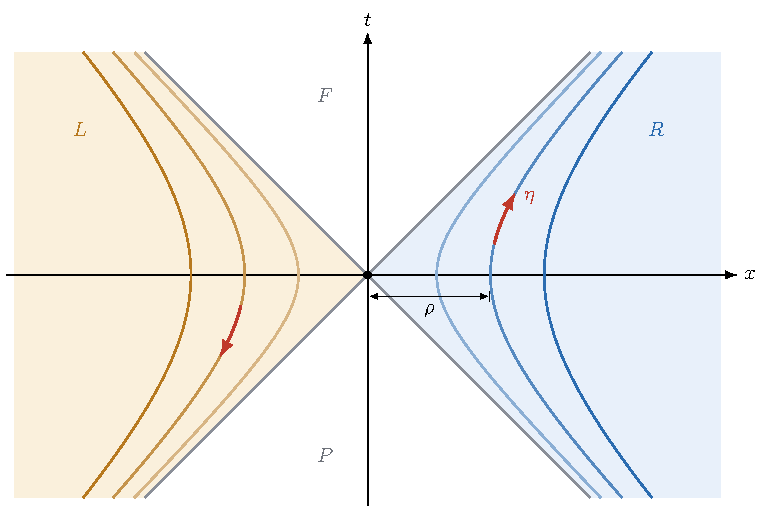
\includegraphics[width=0.82\textwidth]{figs/fig_rindler.pdf}
\caption{The spacetime geometry of the Rindler wedge: Minkowski spacetime split into the Right wedge $R$ ($x > |t|$), Left wedge $L$ ($x < -|t|$), Future $F$, and Past $P$. The boost hyperbolae $x^2 - t^2 = \rho^2$ represent trajectories of uniformly accelerated observers with proper acceleration $a = 1/\rho$, whose proper time $\tau = \rho \eta$ is governed by the boost parameter $\eta$.}
\label{fig:rindler}
\end{figure}

The \textbf{Reeh--Schlieder theorem} — stated here as a fact, with the intuition given, and used repeatedly
from here to the end of the paper — says: in a relativistic quantum field theory, acting on the vacuum
$\ket\Omega$ with operators localized in \emph{any} open spacetime region (however small) produces a set of
states that is dense in the entire Hilbert space. Applied here, this guarantees $\ket\Omega$ is cyclic with
respect to both $\M_R$ and $\M_L$, and hence — by the cyclic-separating duality established in Sec.~IV.A —
cyclic \emph{and} separating with respect to $\M_R$ alone. So Tomita--Takesaki theory applies directly, with
no further assumption needed.

Here is the genuinely striking physical fact, arrived at by using remark (d) from Sec.~IV.A above (find
\emph{any} generator satisfying the KMS condition, and it must be \emph{the} modular operator, since
uniqueness is guaranteed): the modular operator for $\M_R$ in the vacuum state turns out to be
\[
K_\Omega \equiv -\log\Delta_\Omega = 2\pi K
\]
(eq.~4.44), where $K$ is the ordinary \textbf{boost generator} — the same operator that generates Lorentz
boosts in special relativity, an honest geometric symmetry of Minkowski space, with absolutely nothing
abstract or algebraic about its definition. Justifying eq.~4.44 requires checking two things, both genuinely
checkable rather than mysterious: (i) flows generated by $K$ are automorphisms of $\M_R$ — immediate, since a
boost maps the Rindler wedge $\widehat R$ to itself (it's a symmetry of the wedge, by the wedge's very
definition as the region left invariant, as a set, by boosts); and (ii) correlators of boosted operators,
$\braket{\Omega|e^{iK\eta}A(x)e^{-iK\eta}B(y)|\Omega}$ for $x,y\in\widehat R$, satisfy the KMS relation with
$\beta=2\pi$ with respect to the boost parameter $\eta$ (eq.~4.45) — a genuine field-theory computation (not
reproduced here) confirming the KMS property directly on physical correlators.

The physical translation of condition (ii) is exactly the \textbf{Unruh effect}, and it's worth spelling out
the geometry carefully, because ``a Rindler observer'' is not just a figure of speech. Writing the Minkowski
metric as $ds^2=-dt^2+dx^2=-\rho^2d\eta^2+d\rho^2$ (Rindler coordinates: $\rho$ is a radial-like coordinate,
$\eta$ a boost-angle-like coordinate), a trajectory of constant $\rho$ traces out a hyperbola in the $(t,x)$
plane — this is exactly the worldline of an observer undergoing constant proper acceleration $a=1/\rho$, and
$\eta$, the boost parameter, is proportional to that observer's own proper time, $d\tau=\rho\,d\eta$.
Condition (ii) says: observers using $\eta$ as their clock — i.e., \emph{exactly these uniformly accelerated
observers} — experience the ordinary Minkowski vacuum, which contains no particles at all as far as an
inertial observer is concerned, as a genuinely thermal bath, at temperature
\[
T_\rho = \frac{1}{2\pi\rho} = \frac{a}{2\pi} .
\]
This is Unruh's 1976 result, arrived at here as a direct, unavoidable consequence of Tomita--Takesaki theory
applied to the vacuum of a relativistic field, with the specific factor of $2\pi$ in eq.~4.44 being exactly
what converts the universal, dimensionless modular temperature $\beta=1$ into this specific, physical
temperature once $\eta$ is converted to the accelerated observer's own proper time $\tau$.

\begin{figure}[htbp]
\centering
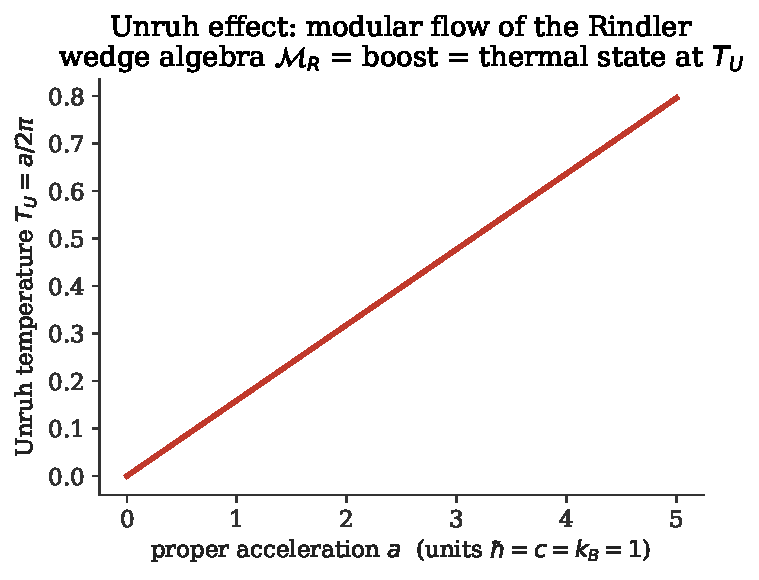
\includegraphics[width=0.78\textwidth]{figs/fig_unruh.pdf}
\caption{The Bisognano--Wichmann theorem and the Unruh effect: the modular flow $\sigma_t^\Omega(A) = \Delta_\Omega^{it} A \Delta_\Omega^{-it}$ acting on the right Rindler wedge $\M_R$ is geometrically equivalent to a Lorentz boost with parameter $\eta = 2\pi t$. Accelerated observers perceive the Minkowski vacuum as a thermal KMS state with local Unruh temperature $T(x) = \hbar c / (2\pi k_B x)$.}
\label{fig:unruh}
\end{figure}

The boost generator $K$ has purely continuous spectrum, all of $(-\infty,\infty)$ (it's the generator of an
honest noncompact symmetry — there's no smallest nonzero boost, and boosts of arbitrarily large rapidity all
exist), so $\Delta_\Omega=e^{-2\pi K}$ has spectrum all of $\mathbb R_{\ge0}$ — and it can be shown that
$S(\M_R)$ coincides with this spectrum, giving (by the classification of Sec.~IV.B) \textbf{$\M_R$ is type
$\mathrm{III}_1$}. The modular conjugation $J_\Omega$ turns out to be exactly $CRT$ — charge conjugation,
combined with a spatial reflection and time reversal — meaning Tomita--Takesaki theory, applied to a
relativistic vacuum, reconstructs the celebrated CPT theorem directly out of nothing but the algebra and the
vacuum state, with no separate argument needed.

This entire story generalizes immediately to higher spacetime dimensions (any transverse directions just ride
along unaffected, since the boost only acts in the $t$-$x$ plane), and — this is the deeper point, worth
holding onto — it generalizes to a \emph{general} open region $O$ on a Cauchy slice, not just the special case
of a half-space. Reeh--Schlieder guarantees $\ket\Omega$ is still cyclic and separating for $\M_O$, so
Tomita--Takesaki theory applies; the modular operator can no longer, in general, be written down in closed
form (it depends on the precise theory and the precise shape of $O$), but a scale-invariance argument (valid
whenever the theory has a scale-invariant UV fixed point — true of essentially any interacting quantum field
theory taken to short enough distances) still pins down its type. The argument: right near the boundary
$\Sigma_O$ of the region $O$, that boundary looks, at short enough distances, just like a flat plane — locally
indistinguishable from the Rindler-wedge geometry just worked out — so
\[
-\log\Delta_\Omega \approx 2\pi K, \qquad \text{very close to } \Sigma_O ,
\]
(eq.~4.46) with $K$ now the boost that locally leaves $\Sigma_O$ fixed, forcing the same continuous spectrum
$\mathbb R_{\ge0}$ and hence, again, type $\mathrm{III}_1$. \textbf{The type $\mathrm{III}_1$ nature of every
local algebra in a relativistic quantum field theory can be traced directly to this local Rindler structure
near any entangling surface, which in turn is a direct consequence of relativistic causal structure itself} —
this is the precise sense in which ``the causal structure of a relativistic QFT requires type
$\mathrm{III}_1$,'' and correspondingly, a \emph{non}-relativistic field theory (with no light-cone structure
forcing this local Rindler behavior near any cut) need not have type $\mathrm{III}_1$ local algebras at all.

\subsubsection*{Sec.~IV.D.2: the split property}

The heuristic picture from Sec.~I — that non-factorization and type III structure come from infinite
entanglement concentrated among short-distance degrees of freedom right at the boundary of a region — can be
made completely precise, and it's worth seeing the precise version, because it resolves what might otherwise
look like a contradiction: how can two regions be infinitely entangled (type III, no factorization) and yet,
intuitively, ``mostly independent'' once you're not sitting exactly on the shared boundary?

Separate $R$ and $L$ by a small but nonzero buffer distance $\epsilon_b$ (so there's a thin strip $I_\epsilon$
of ``no man's land'' between them). The \textbf{split property} states that there \emph{is} a genuine tensor
factorization $\HH=\HH_1\otimes\HH_2$, with
\[
\M_R \subset B(\HH_1)\otimes\id_{\HH_2} \subset \M_L' = \M_{R_\epsilon}, \qquad
\M_L \subset \id_{\HH_1}\otimes B(\HH_2) \subset \M_R' = \M_{L_\epsilon}
\]
(eq.~4.47, where $R_\epsilon\equiv R\cup I_\epsilon$, similarly $L_\epsilon$) — a genuine type I factor,
$B(\HH_1)\otimes\id_{\HH_2}$, sandwiched in between the two type $\mathrm{III}_1$ algebras $\M_R$ and
$\M_{R_\epsilon}$. This says something with real physical bite: once $R$ and $L$ are separated by \emph{any}
nonzero distance, however small, they \emph{can} be completely disentangled — there exist genuine, honest
product states with respect to the factors $\HH_1,\HH_2$, on which $\M_R$ and $\M_L$ act purely separately.
The entanglement obstruction from Sec.~I, in other words, is a purely short-distance, boundary-localized
phenomenon; it evaporates completely the instant you step back even an infinitesimal amount from the shared
edge. More generally, for any two regions $O_1\subset O_2$ whose boundaries don't actually touch (the closure
of $O_1$ sits strictly inside the interior of $O_2$), the split property guarantees a genuine type I factor
$\N$ with $\M_{O_1}\subset\N\subset\M_{O_2}$ (eq.~4.48) — a type I ``buffer'' can always be inserted, as long
as there's any geometric gap at all to insert it into.

The split property is not an extra assumption pulled from nowhere; it can be shown to follow from a technical
condition called the \emph{nuclear property} — a statement about how quickly the theory's energy density
grows at high energies — believed to hold for any ``reasonable'' relativistic QFT. Given the split property,
it can further be shown that $\M_O$, for an open region $O$, is not just type $\mathrm{III}_1$ but also
\textbf{hyperfinite}: it can be built as the weak closure of an increasing sequence of ordinary,
finite-dimensional matrix algebras (exactly the kind of construction used throughout this companion — bigger
and bigger, but always finite, matrices, taken to a limit). A deep uniqueness theorem then applies: hyperfinite
type $\mathrm{III}_1$ von Neumann algebras are, up to isomorphism, all the \emph{same} algebra. The striking
consequence: \textbf{the local algebra of any region in any ``reasonable'' relativistic QFT — free or
interacting, weakly or strongly coupled, any spacetime dimension — is abstractly isomorphic to the local
algebra of any other region in any other such theory.} Different theories are distinguished not by what their
local algebras \emph{are} (abstractly, they're all the same object), but by how those algebras sit relative to
one another — which operators are shared between overlapping regions, how correlators between distant regions
behave, and so on. This is a genuinely surprising, almost counter-intuitive statement, and it's stated here
exactly as strongly as the paper states it, because it's one of the cleanest illustrations of how much
structure the type classification alone captures, and how much it deliberately does \emph{not} capture (the
dynamics, which lives entirely in the relations between algebras, not in any single algebra's abstract type).

Two further, related consequences are worth walking through, because the first comes with an actual proof
sketch worth seeing, and the second is one of the more startling facts in the whole paper.

\textbf{Strong local preparability.} Take the setup of Fig.~5 (regions $R,L$ split by a buffer $I_\epsilon$).
For a general state $\omega$, there's generally a genuine correlation between $R$ and $L$-operators,
$\omega(AB)\ne\omega(A)\omega(B)$ for $A\in\M_R,B\in\M_L$ (eq.~4.49) — nothing surprising there. The startling
claim: using an operation $W$ supported only in the slightly enlarged region $R_\epsilon$ (not $R$ itself, but
$R$ plus the thin buffer strip), it is possible to build a \emph{new} state $\omega_W$ that (i) has
\emph{zero} correlation between $\M_R$ and $\M_L$ at all, and (ii) matches some arbitrarily chosen target
state $\phi$ exactly on $\M_R$, while leaving the state on $\M_L$ completely unchanged from the original
$\omega$ (eqs.~4.50--4.51). This sounds like it should be nearly impossible — locally erase all correlation
with a distant system while simultaneously re-preparing your own region into any state you like, without
touching the distant system at all — and yet it follows in a few lines from the split property and the type
III structure. Here is the argument, worth seeing because it's short: by the split property, $\M_R\subset
B(\HH_1)$, so there's a vector $\ket\xi\in\HH_1$ representing the target state, $\phi(A)=\braket{\xi|A|\xi}$
(justified more carefully in Sec.~IV.G below). The projection $P_\xi=\ket\xi\rangle\langle\xi|\otimes
\id_{\HH_2}$ lies in $\M_{R_\epsilon}$; since $\M_{R_\epsilon}$ is type III, \emph{every} nonzero projection in
it is equivalent to the identity (Sec.~II.B.5's finiteness discussion, pushed to its extreme: in type III,
nothing is finite, so everything is as ``big'' as the whole algebra) — so there's an isometry $W\in
\M_{R_\epsilon}$ with $WW^\dagger=P_\xi$, $W^\dagger W=\id$. Because $W\in\M_{R_\epsilon}\subset\M_L'$, it
commutes with everything in $\M_L$, so $\omega_W(B)\equiv\omega(W^\dagger BW)=\omega(B)$ for $B\in\M_L$
(eq.~4.51) — the $L$-side is untouched, exactly as claimed. And a short algebraic manipulation using
$P_\xi AP_\xi=\phi(A)P_\xi$ (immediate from $\ket\xi$ representing $\phi$) gives $W^\dagger AW=\phi(A)\id$
(eq.~4.52), from which $\omega(W^\dagger ABW)=\phi(A)\omega(B)$ follows directly (eq.~4.53) — exactly the
claimed factorized, re-prepared state.

\textbf{The Connes--St\o rmer transitivity theorem.} For a type $\mathrm{III}_1$ factor, \emph{any} two states
$\phi,\omega$ can be connected to arbitrary precision $\epsilon>0$ by a unitary $W$ \emph{living inside the
algebra itself}, $\|\phi-\omega_W\|<\epsilon$ (eq.~4.54). In words: every state can be prepared, locally, to
arbitrary accuracy, starting from any other state — a statement of ergodicity so strong it's fair to call the
resulting state space \emph{homogeneous}: no state is structurally special or hard to reach from any other,
in sharp contrast to a type I algebra with a nontrivial center, where different superselection sectors are, by
definition, mutually unreachable by anything in the algebra.

\subsubsection*{Sec.~IV.D.3: the collection of algebras $\{\M(O)\}$, and Haag duality}

One closing structural point, worth having on hand because it resurfaces directly in Sec.~VII: the full
collection of local algebras $\{\M(O)\}$, one for every open spacetime region $O$, is expected to satisfy
several basic consistency relations, each one a direct algebraic translation of an ordinary physical
principle. \textbf{Isotony}, $\M(O_1)\subseteq\M(O_2)$ for $O_1\subseteq O_2$ (eq.~4.55): a bigger region
gives access to at least as many operations as a smaller one it contains — this is almost definitional.
\textbf{The time-slice axiom}, $\M(O)=\M(\widehat O)$ (eq.~4.56): because the equations of motion are causal,
operators anywhere in the domain of dependence $\widehat O$ can be re-expressed, via time evolution, in terms
of operators in $O$ itself — so knowing the algebra on a single Cauchy slice already determines it everywhere.
\textbf{Locality (commutativity)}, $\M(O')\subseteq\M(O)'$ (eq.~4.57): operators in the causal complement
$O'$ (spacelike separated from all of $O$) commute with everything in $\M(O)$ — the operator-algebra statement
of ordinary microcausality. When this last relation holds with \emph{equality}, $\M(O')=\M(O)'$, it's called
\textbf{Haag duality} (eq.~4.58) — a strictly stronger statement, saying that literally \emph{every} operator
commuting with $\M(O)$ is already accounted for by the causal complement, with nothing extra hiding outside
that count. Haag duality is not automatic (it can fail for topologically nontrivial regions), but is expected
to hold quite generally for the vacuum sector of an ordinary relativistic QFT on topologically simple regions.
Two further relations — \textbf{additivity}, $\M(O_1\cup O_2)=\M(O_1)\vee\M(O_2)$ (eq.~4.60: no ``extra,''
genuinely nonlocal operators hide in a union that aren't already built from the pieces), and the resulting
\textbf{intersection property}, $\M(O_1\cap O_2)=\M(O_1)\cap\M(O_2)$ (eq.~4.61, which follows from combining
Haag duality and additivity via a short commutant manipulation, eqs.~4.62--4.63) — round out the full package.
A theory satisfying all of these, for every region (not just topologically trivial ones), is called
``complete.'' These relations are worth having memorized in outline, not for their own sake, but because
Sec.~VII builds subregion-subalgebra duality directly on top of exactly this dictionary, translated to the
boundary theory of AdS/CFT.

\subsection{Sec.~IV.E: emergent times from subalgebras — half-sided modular inclusion}

This subsection introduces a second, genuinely distinct notion of emergent time — one that comes not from a
single algebra's own modular flow, but from the relationship between an algebra and a carefully chosen
subalgebra of it. It is a unique feature of type $\mathrm{III}_1$ algebras specifically, and it is exactly the
mechanism, picked up again in Sec.~VII, that lets a single band of boundary time generate the entire interior
of an emergent black-hole horizon.

\subsubsection*{A new, positive ``Hamiltonian'' $G$}

Let $\M$ be a von Neumann algebra with cyclic-separating vector $\ket\Omega$, modular data $\Delta_\M=
e^{-K_\M}$, $J_\M$, as in Sec.~IV.A. Now suppose $\N\subset\M$ is a genuine subalgebra, and $\ket\Omega$
happens to \emph{also} be cyclic for $\N$ (automatically separating too, since $\N\subset\M$ and $\ket\Omega$
is already separating for the bigger algebra $\M$). $\N$ inherits its own modular data, $\Delta_\N=e^{-K_\N}$,
$J_\N$, with respect to the same $\ket\Omega$.

Here is the first new structural fact, and it's worth seeing the one-line reason it's true: because $\N\subset
\M$, the Tomita operator $S_\M$ (built from $\M$ and $\ket\Omega$) is literally an extension of $S_\N$ (built
from the smaller algebra $\N$ and the same $\ket\Omega$) — $S_\M$ agrees with $S_\N$ everywhere $S_\N$ is
defined, but is also defined on the larger domain $\M\ket\Omega\supseteq\N\ket\Omega$. A general fact about
unbounded operators (extending an operator can only make $X^\dagger X$ bigger, never smaller, in the operator
ordering sense) then gives $\Delta_\N\ge\Delta_\M$ (eq.~4.64), i.e., using $-\log$ (which reverses
inequalities for positive operators), $K_\M\ge K_\N$. Define
\[
G \equiv \frac{1}{2\pi}(K_\M-K_\N) \ \ge 0, \qquad G\ket\Omega=0
\]
(eq.~4.65 — the $2\pi$ is just a convenient normalization chosen for what follows; $G\ket\Omega=0$ follows
because both $K_\M$ and $K_\N$ individually annihilate $\ket\Omega$, eq.~4.9 applied to each). $G$ is a
genuinely positive operator, so it deserves to be called a Hamiltonian, and the flow $e^{iGs}$ it generates is
a legitimate new notion of ``time'' — a second one, distinct from either $\M$'s own modular flow or $\N$'s —
that also happens to leave the reference vector $\ket\Omega$ fixed.

\subsubsection*{The half-sided modular inclusion condition, and what it buys you}

Everything so far works for \emph{any} subalgebra $\N\subset\M$ sharing a cyclic-separating vector. Something
much stronger becomes available if $\N$ satisfies one additional geometric-looking condition, called
\textbf{half-sided modular inclusion}:
\[
\N_t \equiv \Delta_\M^{-it}\N\Delta_\M^{it} \subset \N, \qquad \text{for every } t\le0
\]
(eq.~4.81) — flowing $\N$ by $\M$'s \emph{own} modular flow, for negative modular time, always shrinks $\N$
(or leaves it the same), never grows it. When this holds, a theorem (due to Wiesbrock and, independently,
Borchers, building on earlier work) establishes three remarkable consequences at once, none of them assumed —
all derived purely from eq.~4.81:

\begin{enumerate}
\item $K_\M$ and $K_\N$ satisfy the commutation relations of a genuine \textbf{two-dimensional conformal
(M\"obius) algebra} together with $G$:
\[
[K_\M,K_\N] = -4\pi^2i\,G , \qquad [K_\M,G] = 2\pi i\,G
\]
(eq.~4.82, with a companion relation for the modular conjugations, eq.~4.83) — an entire, recognizable piece
of two-dimensional conformal symmetry, produced out of nothing but one algebraic inclusion condition on two
von Neumann algebras.
\item The flow generated by $G$ moves $\M$ into itself for one whole half of the time axis: $e^{iGs}\M
e^{-iGs}\subset\M$ for $s<0$ (eq.~4.84), and in particular $\N=e^{-iG}\M e^{iG}$ (eq.~4.85) — $\N$ is exactly
the image of $\M$ under one unit of this new, $G$-generated time translation. Running $G$ continuously
produces a whole nested, continuously-parametrized family $\N_t\equiv e^{-iGt}\M e^{iGt}$, with $\N_{t_1}
\subset\N_{t_2}\subset\M$ for $t_1<t_2$ and $\N_\infty=\M$ (eqs.~4.89--4.90) — genuinely new time translation,
distinct from $\M$'s own modular flow, acting purely by relating the algebra to smaller and smaller versions
of itself.
\item \textbf{$\M$ must be type $\mathrm{III}_1$.} Half-sided modular inclusion is not just a convenient
technical condition — its very existence forces the ambient algebra to be the ``most chaotic'' type
identified back in Sec.~IV.B.
\end{enumerate}
(The paper builds several further technical objects along the way to this theorem — unitaries $D(t)=\Delta_\M
^{-it}\Delta_\N^{it}$, $V=J_\M J_\N$, and a chain of nested algebras built by repeatedly conjugating with $V$,
eqs.~4.66--4.80 — used to actually \emph{prove} the theorem and to establish that this half-sided-inclusion
structure, once it exists, is completely unique. These are genuine, careful pieces of functional analysis;
they're flagged here so the notation isn't a surprise if you look at the original, but the three numbered
consequences above are the physical content that matters for everything downstream.)

\subsubsection*{The concrete example: light-cone translations in the Rindler wedge}

Here is the worked example the paper gives, and it's worth working through fully, because it turns the
abstract theorem above into something you can literally picture. Take $\M$ to be the algebra of the right
Rindler wedge $\widehat R$ from Sec.~IV.D.1, and let $\N$ be the algebra of the smaller region $\{x^+>0,\,
x^-<-1\}$ (using light-cone coordinates $x^\pm=x^0\pm x^1$) — a wedge-shaped region nested strictly inside
$\widehat R$, shifted over by one unit along the $x^-$ direction (Fig.~6, left panel). Using $K_\M=2\pi K$
(the boost generator, eq.~4.44) to flow $\N$: because a boost acts on light-cone coordinates by simple
rescaling, $x^\pm\to e^{\mp\eta}x^\pm$, flowing the defining condition $x^->-1$ for time $t$ using
$e^{iK_\M t}=e^{2\pi iKt}$ turns it into $x^->-e^{-2\pi t}$ — so
\[
\N_t \equiv e^{iK_\M t}\N e^{-iK_\M t} = \text{algebra of the region } \{x^+>0,\,x^-<-e^{-2\pi t}\}
\]
(eq.~4.95), and since $e^{-2\pi t}>1$ for $t<0$, this region is genuinely \emph{smaller} than the original
$\N$ (it requires $x^-$ to be even more negative) — exactly $\N_t\subset\N$ for $t<0$, precisely the
half-sided modular inclusion condition, verified directly on an explicit geometric example rather than just
asserted abstractly.

Identifying $G$ explicitly here is a short computation using the ordinary Poincar\'e algebra you already know
from special relativity: writing $P^\pm=\tfrac12(P^0\pm P^1)$ for the light-cone components of the momentum
(energy-momentum) operator, the standard commutation relation between the boost generator and momentum,
$[K,P^\pm]=\pm iP^\pm$ (eq.~4.97 — this is just the ordinary statement that a boost rescales energy and
momentum, exactly the way it rescales light-cone coordinates), combined with the definition of $K_\N$ via a
translation of $K_\M$ by the fixed point $a^\mu=(0,-1)$ of $\N$'s own boost symmetry (eq.~4.96), gives directly
\[
K_\N = K_\M - 2\pi P^+ \qquad \Longrightarrow \qquad G = P^+
\]
(eqs.~4.98--4.99, using the definition $G=\tfrac1{2\pi}(K_\M-K_\N)$ from eq.~4.65). \textbf{So in this example,
the abstract ``positive Hamiltonian'' $G$ is nothing more exotic than the ordinary light-cone momentum
operator $P^+$, and the abstract new ``time flow'' it generates is nothing more exotic than ordinary
translation in the $x^-$ direction.} Every one of the general statements 1--3 above (the conformal algebra,
the half-sided translation structure, the forced type $\mathrm{III}_1$ conclusion) can be checked directly on
this example using nothing but ordinary special-relativistic kinematics — and this is exactly the mechanism
that Sec.~VIII will reuse, essentially verbatim, to show that a single band of \emph{boundary} time in
AdS/CFT can generate the entire interior of an emergent black-hole horizon: the interior turns out to be built
by exactly this kind of half-sided-modular-inclusion light-cone translation, with $G$ playing the role of a
genuine, positive bulk momentum.

(One further variant, quickly: taking $\N$ to instead be the region in Fig.~6's right panel gives a half-sided
inclusion on the \emph{positive} $t$-axis instead, $\N_t\subset\N$ for $t\ge0$ eq.~4.92, with correspondingly
sign-flipped relations eq.~4.93--4.94, and a modular translation generator $G=P^-$ instead of $P^+$ — the
mirror-image construction, translating in $x^+$ instead of $x^-$.)

\subsection{Sec.~IV.F: relative modular flows and relative entropy}

Everything in this subsection is a direct generalization of the material already met in Sec.~I (relative
entropy $S(\rho\|\sigma)$) and Sec.~IV.A (the Tomita operator $S_\Psi$) to a version involving \emph{two}
different reference states $\ket\Psi,\ket\Omega$ at once, both cyclic and separating for the same $\M$. The
goal, worth keeping in view through the machinery: produce a version of relative entropy that survives even
when $\M$ is type III (where, as emphasized since Sec.~III, ordinary entropy $S_\M$ cannot be defined at all).

Define a \textbf{relative Tomita operator} exactly analogously to before, but now mapping between the two
reference vectors:
\[
S_{\Psi\Omega}A\ket\Omega = A^\dagger\ket\Psi\ \ (A\in\M), \qquad
S_{\Psi\Omega}A'\ket\Omega = A'^\dagger\ket\Psi\ \ (A'\in\M')
\]
(eq.~4.100), with polar decomposition $S_{\Psi\Omega}=J_{\Psi\Omega}\Delta_{\Psi\Omega}^{1/2}$ (eq.~4.102)
defining the \textbf{relative modular operator} $\Delta_{\Psi\Omega}\ge0$ and \textbf{relative modular
conjugation} $J_{\Psi\Omega}$, exactly the way the ordinary versions were built in Sec.~IV.A, but now
genuinely mixing the two states. (A short algebraic identity, $S_{\Psi\Omega}S_{\Omega\Psi}=\id$, eq.~4.101,
following directly from the definition, forces a relation $J_{\Psi\Omega}=J_{\Omega\Psi}^\dagger$ and
$J_{\Psi\Omega}\Delta_{\Psi\Omega}J_{\Psi\Omega}=\Delta_{\Omega\Psi}^{-1}$, eqs.~4.103--4.104 — a genuine
consistency check, worked out from the polar-decomposition uniqueness, but not needed for what follows.) There
is a two-state generalization of the KMS relation,
\[
\braket{\Psi|AB|\Psi} = \braket{\Omega|B\,\Delta_{\Psi\Omega}\,A|\Omega}, \qquad A,B\in\M
\]
(eq.~4.105, whose short proof, eq.~4.106, is just unpacking the definition of $S_{\Psi\Omega}$ on both
sides) — this single relation lets you convert correlation functions computed in one state, $\ket\Psi$,
directly into correlation functions computed in the other, $\ket\Omega$, and vice versa: genuinely useful
machinery, used freely later without re-derivation whenever the paper needs to compare correlators across two
different reference states.

The flow generated by $\Delta_{\Psi\Omega}$ can be shown to coincide, on $\M$, with the flow generated by the
ordinary (single-state) $\Delta_\Psi$, and on $\M'$ with the flow generated by $\Delta_\Omega$ (eqs.~4.107--
4.108) — and a further intertwining unitary $u_{\Omega\Psi}(s)\equiv\Delta_{\Omega\Phi}^{-is}\Delta_{\Psi\Phi}
^{is}$ (eq.~4.109, built using a third, auxiliary reference $\ket\Phi$, but shown to not actually depend on
which $\Phi$ was used) gives an \emph{explicit construction} of the inner automorphism relating $\sigma_s^\Psi$
and $\sigma_s^\Omega$ promised back in eq.~4.23 of Sec.~IV.B — closing a loop left open there. (A further
family of identities, eqs.~4.110--4.116, work out consistency relations and alternative expressions for these
intertwiners; they are used as technical machinery later and are not reproduced here.)

\subsubsection*{The payoff: relative entropy for type III, and a genuine positivity proof}

Here, finally, is the object that survives everything: for a type III algebra $\M$, no entropy $S_\M(\Omega)$
can be assigned to a single state $\Omega$ — but a \textbf{relative} entropy between two states can be, using
the relative modular operator just constructed:
\[
S_\M(\Psi\|\Omega) \equiv -\braket{\Psi|\log\Delta_{\Omega\Psi}|\Psi} .
\]
(eq.~4.117.) When $\M$ does have a trace (type I or II, with $\Delta_{\Omega\Psi}=\rho_\Omega\rho_\Psi'^{-1}$
in terms of density operators, eq.~4.118), this reduces exactly to the familiar formula
\[
S_\M(\Psi\|\Omega) = \tr(\rho_\Psi\log\rho_\Psi) - \tr(\rho_\Psi\log\rho_\Omega)
\]
(eq.~4.119, matching eq.~1.8 of Sec.~I of this companion) — but eq.~4.117 itself needs no trace to be
well-defined, and survives, completely intact, into type III.

It's worth seeing the positivity of this relative entropy actually proved, rather than just asserted, since it
is short and genuinely instructive: using the elementary calculus inequality $\log x\le x-1$ (true for every
positive real $x$, with equality only at $x=1$ — a fact you can check by noting $f(x)=x-1-\log x$ has
$f(1)=0$ and $f'(x)=1-1/x$, which is negative for $x<1$ and positive for $x>1$, so $x=1$ is the unique global
minimum of $f$, where $f=0$),
\[
-\braket{\Psi|\log\Delta_{\Omega\Psi}|\Psi} \ \ge\ \braket{\Psi|1-\Delta_{\Omega\Psi}|\Psi}
\ =\ -\braket{\Psi|\Psi} + \braket{\Omega|\Omega} \ =\ 0
\]
(eq.~4.120), where the middle equality uses the two-state KMS relation (eq.~4.105) applied with $A=B=\id$, and
the final equality is just $\braket{\Psi|\Psi}=\braket{\Omega|\Omega}=1$ (both are normalized states). So
$S_\M(\Psi\|\Omega)\ge0$ always — the relative entropy is never negative — proved here using nothing beyond
one calculus inequality and the KMS relation already established. This non-negativity is worth contrasting
directly with Sec.~III's finding that the ordinary (non-relative) entropy $S_\M$, in a type II algebra, could
come out negative: relative entropy is the more robust, better-behaved object precisely because it's always
measuring distinguishability from a fixed, explicit reference, never trying to count states from some absolute
zero that a type II or III algebra simply doesn't have.

\subsection{Sec.~IV.G: a canonical purification — the natural cone}

This closing, more technical subsection answers a question that was quietly used without justification in the
strong-local-preparability proof above (Sec.~IV.D.2): given a state $\omega$ on $\M$, is there a
\emph{canonical} choice of purifying vector $\ket\xi\in\HH$ with $\omega(A)=\braket{\xi|A|\xi}$ — and can it
always be chosen to represent a genuine (not just formal) vector?

In general there can be infinitely many different purifying vectors for the same $\omega$ (a simple type I
example: for $\M=B(\HH_1)\otimes\id_{\HH_2}$, any vector in $\HH_1\otimes\HH_2$ that reduces to the right
density matrix on $\HH_1$ works, pure or mixed, and there's no reason to prefer one over another in general).
But if $\HH$ happens to contain \emph{some} cyclic-separating vector for $\M$ at all (a condition called being
in \textbf{standard form} — satisfied, for instance, whenever $\M=\M_O$ for an open region $O$ in the vacuum
sector of a relativistic QFT, courtesy of Reeh--Schlieder, and satisfied automatically by any GNS
representation built from a faithful state, Sec.~II.D), then a genuinely canonical purifying vector
$\ket{\xi_\omega}$ exists (eq.~4.121).

It's constructed as follows: given a fixed cyclic-separating reference $\ket\Omega$, define the \textbf{natural
cone} $P_\Omega$ as the closure of the set $\{Aj_\Omega(A)\ket\Omega : A\in\M\}$, where $j_\Omega(A)\equiv
J_\Omega AJ_\Omega$ (eq.~4.122; an equivalent description, eq.~4.123, is the closure of
$\{\Delta_\Omega^{1/4}A^\dagger A\ket\Omega : A\in\M\}$). Every normal state $\omega$ on $\M$ then has a
\emph{unique} representative vector inside $P_\Omega$ — this is the canonical purification. (It depends on the
choice of $\Omega$ used to build the cone in the first place; a different reference vector gives, in general,
a different natural cone and hence a different canonical purification of the same $\omega$.)

The paper lists several further technical properties of vectors in the natural cone (eqs.~4.124--4.134) — that
inner products between any two vectors in $P_\Omega$ are automatically real and non-negative (eq.~4.126, the
property actually used in the strong-local-preparability argument above, and the one worth remembering); a
decomposition property for vectors fixed by $J_\Omega$ (eq.~4.127); a distance bound relating the vector-space
distance between two purifications to the more abstract distance between the two states they represent
(eq.~4.128); the fact that any two different cyclic-separating vectors within the same natural cone share
\emph{all} of their modular data — the same $J$, the same cone (eqs.~4.129--4.131); how to handle a
cyclic-separating vector that sits \emph{outside} the natural cone, by relating it back with an explicit
unitary correction (eq.~4.132); and the fact that every automorphism of $\M$ can be implemented by a unitary
chosen to preserve the natural cone (eqs.~4.133--4.134). These are the technical tools that make later,
more advanced arguments in the paper watertight; the property that actually matters for the physical content
of this companion is the existence-and-uniqueness statement itself (eq.~4.121) and the positivity property
(eq.~4.126) — both used explicitly already, above.

\bigskip
\noindent This closes Sec.~IV, and with it, every tool needed to talk about entanglement for \emph{any} type
of von Neumann algebra — I, II, and now III. Section~V picks up exactly where remark (f) of Sec.~IV.A left
off: type III has no trace and hence no entropy of its own, which is a real problem if the goal is ever to
compute something like a black-hole entropy using this machinery. The \textbf{crossed product}, introduced
next, is the construction that fixes this — by literally attaching an auxiliary quantum system (a clock) to a
type III algebra and turning it into a type II algebra, which \emph{does} have a trace.

\section{Sec.~V: Crossed product by modular group}

Section~IV ended on a genuinely uncomfortable note: type III algebras have no trace, so there is no density
operator and no entropy for them at all — not even the signed, relative-to-a-reference kind that rescued type
II in Sec.~III. If the eventual goal is to compute something like a black-hole entropy using nothing but
operator algebra, this is a real obstruction, not a cosmetic one. The \textbf{crossed product} is the
construction that removes it — not by cheating around the no-trace theorem, but by building a genuinely
\emph{different, larger} algebra, out of the original type III one, that turns out to always be type II (which
does have a trace). The mechanism, remarkably, is completely mechanical and general-purpose, and it will
reappear, essentially unchanged, as the actual physical mechanism behind gravitational entropy starting in
Sec.~IX.

\subsection{Sec.~V, opening: crossed products in general}

Here is the general-purpose construction, stated first without any reference to modular theory at all, because
it's a standard piece of operator-algebra machinery on its own, and it's worth seeing that the specific
application to modular flow (the one this paper actually needs) is just one instance of it. Suppose a group
$G$ acts on a von Neumann algebra $\M$ by unitaries, $\alpha_g(A)=U_gAU_g^\dagger$ (eq.~5.1) — some
one-parameter (or more general) family of symmetries of $\M$. Given the triple $(\M,G,\alpha)$, there is a
standard construction, called the \textbf{crossed product} $\widehat\M\equiv\M\rtimes_\alpha G$, that builds a
\emph{new} von Neumann algebra acting on the enlarged Hilbert space $\widehat\HH=\HH\otimes L^2(G)$ (functions
on $G$, valued in $\HH$ — think of it as attaching an auxiliary quantum system whose configuration space is
$G$ itself). For the case of interest here, $G=\mathbb R$ with generator $K$ and action $\alpha_t(A)=
e^{iKt}Ae^{-iKt}$ (eq.~5.2), so $\widehat\HH=\HH\otimes L^2(\mathbb R)$ — an auxiliary particle on a line.

The specific case this paper needs, and the only one used from here on, takes $K=-\log\Delta_\Psi$ — the
\emph{modular} generator of $\M$ itself, for some cyclic-separating $\ket\Psi$ — so that eq.~5.2 is exactly
the modular flow $\sigma_t$ already built in Sec.~IV. The headline result, proved step by step below: for a
type III algebra $\M$, the resulting crossed product $\widehat\M$ is \textbf{always type II} — regardless of
which type III subtype $\M$ started as. This immediately buys back everything Sec.~III's machinery (density
operators, entropy) needs, applied now to $\widehat\M$ instead of $\M$ itself. And — a fact worth flagging
immediately, even though it's only fully justified at the end of Sec.~V.B — $\widehat\M$ turns out to depend
only on the algebra $\M$, not on which reference state $\ket\Psi$ was used to build the modular flow that
crossed it — so this is really a construction \emph{intrinsic} to $\M$, not an artifact of an arbitrary
choice. This is also, as flagged already back in Sec.~I, exactly the mechanism used in Sec.~IX to explain
black-hole and de~Sitter entropy: there, $\hat q$ below will literally be a physical observer's clock Hamiltonian.

\subsection{Sec.~V.A: construction of \texorpdfstring{$\widehat\M$}{\^M}}

Attach a genuine one-dimensional quantum system — a particle on a line, with position $\hat q$ and momentum
$\hat p$ satisfying the ordinary canonical commutation relation $[\hat q,\hat p]=i$ (eq.~5.3) — to the original
system, giving the enlarged Hilbert space $\HH\otimes L^2(\mathbb R)$. Define the single operator
\[
C \equiv K+\hat q
\]
(eq.~5.4), and let $\widehat\M$ be the subalgebra of $\M\otimes B(L^2(\mathbb R))$ consisting of everything
that commutes with $C$: $a\in\widehat\M$ iff $[a,C]=0$. It's worth pausing on why this particular condition is
the physically right one to impose, since it isn't obvious on sight. $C$ generates \emph{simultaneous}
translations: shifting $\hat q$ by some amount while also flowing modular time by the same amount (since $K$
generates the modular flow and $\hat q$ generates ordinary translations on $L^2(\mathbb R)$, $e^{iCs}$
translates both at once). Demanding invariance under $C$ is exactly demanding that only the \emph{relative}
reading of ``clock minus modular time'' matters, not either one separately — mathematically identical to the
familiar physics idea that only relative position matters, never an absolute coordinate origin. Physically,
in the applications of Sec.~IX, $\hat q$ will be an observer's own energy and $\hat p$ their proper time, and
this invariance condition becomes exactly the statement that physical observables must be
diffeomorphism-invariant (unable to depend on an arbitrary choice of where to put a clock's zero).

Two families of operators manifestly satisfy $[a,C]=0$, and it can be shown they generate the whole of
$\widehat\M$. First, $\hat q$ itself trivially commutes with $C=K+\hat q$ (since $[\hat q,\hat q]=0$ and
$\hat q$ acts on a different factor than $K$), so any (Weyl-form, since $\hat q$ is unbounded) function of it,
$e^{-i\hat qs}$, belongs to $\widehat\M$. Second — and this is the nontrivial part — ordinary elements $A\in
\M$ do \emph{not} commute with $C$ on their own (since $[A,K]\ne0$ in general — that's exactly what it means
for $K$ to generate a nontrivial flow on $A$), but a specific \emph{dressed} version of them does:
\[
[e^{iK\hat p}Ae^{-iK\hat p},\,C] = 0, \qquad A\in\M
\]
(eq.~5.5). Let us prove this commutator identity directly using ordinary canonical commutation relations. Let $\widehat A \equiv e^{iK\hat p}(A\otimes\id)e^{-iK\hat p}$. Using $[\hat q,\hat p]=i$, the position operator acts as a derivative in momentum space: $[\hat q, f(\hat p)] = i f'(\hat p)$. Applying this to the clock translation operator:
\[
[\hat q, \, e^{iK\hat p}] = i(iK)e^{iK\hat p} = -K e^{iK\hat p}, \qquad [\hat q, \, e^{-iK\hat p}] = i(-iK)e^{-iK\hat p} = K e^{-iK\hat p} .
\]
Now compute the commutator $[\hat q, \widehat A]$ using the Leibniz product rule:
\begin{align*}
[\hat q, \, \widehat A] &= [\hat q, \, e^{iK\hat p}](A\otimes\id)e^{-iK\hat p} + e^{iK\hat p}(A\otimes\id)[\hat q, \, e^{-iK\hat p}] \\
&= -K e^{iK\hat p}(A\otimes\id)e^{-iK\hat p} + e^{iK\hat p}(A\otimes\id) e^{-iK\hat p} K \\
&= -K \widehat A + \widehat A K = -[K, \, \widehat A] .
\end{align*}
Therefore, evaluating the commutator with the total constraint $C = K + \hat q$:
\[
[C, \, \widehat A] = [K + \hat q, \, \widehat A] = [K, \, \widehat A] + [\hat q, \, \widehat A] = [K, \, \widehat A] - [K, \, \widehat A] = 0 !
\]
The modular-flow dressing by the clock's momentum $\hat p$ exactly cancels the non-commutativity with $K$, ensuring that $\widehat A$ is strictly invariant under $C$.
So
\[
\widehat\M = \big\{e^{iK\hat p}Ae^{-iK\hat p},\ e^{-i\hat qs} \ \big|\ A\in\M,\ s\in\mathbb R\big\}''
\]
(eq.~5.6), and a general element has the schematic form $\widehat A=\int ds\,A(\hat p;s)\,e^{-i\hat qs}$
(eq.~5.7), with $A(\hat p;s)\equiv e^{iK\hat p}A(s)e^{-iK\hat p}$ built from an operator-valued function
$A(s)\in\M$ — since $\hat p$ is now an operator, $A(\hat p;s)$ is a genuine operator-valued ``function of an
operator,'' living in a kind of quantum spacetime.

There's a second, equivalent way to present the same algebra, obtained by a unitary change of frame
$U=e^{-iK\hat p}$ (which conjugates $\widehat\M\to U\widehat\M U^\dagger$, $C\to UCU^\dagger$), and this
alternative form turns out to be more convenient for essentially everything that follows:
\[
\widehat\M = \big\{A,\ e^{i(K-\hat q)s} \ \big|\ A\in\M,\ s\in\mathbb R\big\}'', \qquad
\widehat A = \int ds\, A(s)\,e^{is(K-\hat q)}, \ A(s)\in\M
\]
(eqs.~5.10, 5.12) — in this frame, ordinary (undressed) elements of $\M$ sit directly inside $\widehat\M$,
and all the dressing has been absorbed into the clock-dependent generator $K-\hat q$ instead.

\subsection{Sec.~V.B: \texorpdfstring{$\widehat\M$}{\^M} is always type II}

\subsubsection*{Finding the modular operator of $\widehat\M$}

Now specialize to $K=-\log\Delta_\Psi$, the genuine modular generator of $\M$, and take the reference vector
\[
\ket{\widehat\Psi} = \ket\Psi\otimes\ket{p=0}
\]
(eq.~5.13, the clock prepared in a definite-momentum, i.e.\ completely spread out in position, state — not
literally normalizable, a technical point flagged in the paper's footnote~30 but not one that affects any
conclusion below). It can be shown $\ket{\widehat\Psi}$ is cyclic and separating for $\widehat\M$, so
Tomita--Takesaki theory applies, and the modular operator $\widehat\Delta$ can be found by directly solving
the defining KMS relation, $\braket{\widehat\Psi|\widehat A\widehat B|\widehat\Psi}=\braket{\widehat\Psi|
\widehat B\,\widehat\Delta\,\widehat A|\widehat\Psi}$ (eq.~5.14), for $\widehat\Delta$ (a computation carried
out in the paper's Appendix~B, not reproduced here). The answer, remarkably simple given how much machinery
went into $\widehat\M$'s construction, is:
\[
\widehat\Delta = \Delta_\Psi
\]
(eq.~5.15) — \textbf{the new algebra's modular operator, in this particular reference state, is exactly the
same operator as the original algebra's modular operator.} Nothing new needed to be invented; the crossed
product inherited its modular structure wholesale.

\subsubsection*{Why this forces type II}

Here is the key algebraic manipulation, and it's short enough to walk through completely. Using
$\widehat\Delta=e^{-K}$ directly:
\[
\widehat\Delta = e^{-K} = e^{-(K-\hat q)}e^{-\hat q} \equiv \rho\rho'^{-1}, \qquad
\rho\equiv e^{-(K-\hat q)}, \quad \rho'\equiv e^{\hat q}
\]
(eq.~5.16), so
\[
\widehat\Delta^{-is} = e^{i(K-\hat q)s}\,e^{i\hat qs}
\]
(eq.~5.17). Now look at what the two factors on the right actually are, comparing against the two presentations
of $\widehat\M$ and $\widehat\M'$ (eqs.~5.10--5.11) given above: $e^{i(K-\hat q)s}$ is manifestly a unitary
sitting inside $\widehat\M$ itself (it's literally one of the generators listed in eq.~5.10), and $e^{i\hat
qs}$ is manifestly a unitary sitting inside $\widehat\M'$ (the commutant, built from eq.~5.11's generators).
\textbf{So $\widehat\Delta^{-is}$ factors as a product of a unitary in $\widehat\M$ times a unitary in
$\widehat\M'$} — which is exactly the criterion (eq.~4.22 of Sec.~IV.B) for the modular flow to be an
\emph{inner} automorphism of $\widehat\M$. But Sec.~IV.B's criterion (eq.~4.21) says modular flow is inner for
\emph{all} $s$ if and only if the algebra is type I or type II — never type III. \textbf{So $\widehat\M$
cannot be type III}, whatever $\M$ itself was. And since $\widehat\HH=\HH\otimes L^2(\mathbb R)$ still cannot
be factorized with respect to $\widehat\M$ (nothing about attaching a clock and imposing an invariance
condition magically produced a tensor factorization — the underlying obstruction from $\M$ is still there),
$\widehat\M$ cannot be type I either. \textbf{By elimination, $\widehat\M$ is type II.} This is worth
appreciating as a genuinely clean piece of reasoning: no explicit trace needed to be constructed to reach this
conclusion — it followed purely from identifying the modular operator and checking the inner-automorphism
criterion already established in Sec.~IV.

\subsubsection*{Building the trace explicitly, and checking cyclicity by hand}

Having established \emph{that} a trace exists, it's worth actually writing one down and checking it really
works, rather than just trusting the general argument. Define
\[
\tr\widehat A \equiv \braket{\widehat\Psi|\widehat A\,\rho^{-1}|\widehat\Psi}
\]
(eq.~5.20, using $\rho=e^{-(K-\hat q)}$ from eq.~5.16 — motivated by the standard fact that if a trace exists,
expectation values in \emph{any} state should look like $\braket{A}=\tr(A\rho_{\text{state}})$ for some density
operator $\rho_{\text{state}}$; solving for what $\rho_{\text{state}}$ would need to be, given that
$\ket{\widehat\Psi}$ is itself the reference state used to build $\Delta_\Psi=\widehat\Delta$, directly
motivates dividing by $\rho$). Cyclicity, $\tr(\widehat A\widehat B)=\tr(\widehat B\widehat A)$, is checked
directly using nothing but the KMS relation (eq.~5.14) that defined $\widehat\Delta$ in the first place:
\[
\tr(\widehat A\widehat B) = \braket{\widehat\Psi|\widehat A\widehat B\rho^{-1}|\widehat\Psi}
= \braket{\widehat B\rho^{-1}\widehat\Delta\,\widehat A} = \braket{\widehat B\rho'^{-1}\widehat A}
= \braket{\widehat B\widehat A\rho'^{-1}} = \tr(\widehat B\widehat A)
\]
(eq.~5.22, suppressing the common $\braket{\widehat\Psi|\cdots|\widehat\Psi}$ for brevity in each term): the
first step is just the definition of $\tr$; the second is the KMS relation (eq.~5.14) applied with the roles
of $A\rho^{-1}$ and $B$ swapped; the third uses $\rho^{-1}\widehat\Delta=\rho^{-1}\rho\rho'^{-1}=\rho'^{-1}$
directly from eq.~5.16's factorization; and the fourth uses that $\rho'^{-1}=e^{-\hat q}\in\widehat\M'$
(established just above) commutes with $\widehat A\in\widehat\M$ by definition of the commutant. Every step is
either a definition or something already established — no new assumption anywhere. This is worth comparing to
the very similar, but much more concrete, cyclicity check already carried out by hand in Sec.~III.C.1
(eqs.~3.12--3.14 of that companion section, for the finite Bell-pair-chain trace): the mechanism is
structurally the same idea (a specific reference state's own consistency conditions force cyclicity), just
now stated in the fully general, type-III-compatible language of modular theory rather than worked out on
explicit small matrices.

\subsubsection*{Type $\mathrm{II}_\infty$, or type $\mathrm{II}_1$ if you restrict the clock's energy}

Compute $\tr(\id)$ directly from eq.~5.21 (an explicit rewriting of eq.~5.20 for the identity element):
\[
\tr(\id) = \int_{-\infty}^{\infty} dq\, e^{-q} \braket{\Psi|\id|\Psi} = \int_{-\infty}^\infty dq\,e^{-q} = \infty
\]
(eq.~5.25) — divergent, so by the Sec.~II.C classification, $\widehat\M$ is (so far) type $\mathrm{II}_\infty$.
But here is a genuinely simple, physically motivated fix, worth seeing in full because it's exactly the
mechanism reused in Sec.~IX: restrict the clock's spectrum to be bounded below, $q\ge0$ — physically, the
statement that a real observer's energy cannot be negative, certainly a reasonable restriction on any
physically sensible clock. Concretely, insert the projector $\Pi=\theta(\hat q)$ (the step function, $1$ for
$q\ge0$ and $0$ for $q<0$) and define $\widehat\M_+\equiv\Pi\widehat\M\Pi$, acting only on the restricted
Hilbert space $\HH\otimes L^2(\mathbb R_{>0})$. The identity of this smaller algebra is $\Pi$ itself, and
\[
\tr_{\widehat\M_+}(\id) = \tr_{\widehat\M}(\Pi) = \int_{-\infty}^\infty dq\,e^{-q}\theta(q) = \int_0^\infty
dq\,e^{-q} = 1
\]
(eq.~5.26) — finite, and in fact already normalized to $1$ with no further rescaling needed. \textbf{So
restricting a physical observer's clock to have positive energy is exactly the algebraic operation that turns
type $\mathrm{II}_\infty$ into type $\mathrm{II}_1$} — a purely mathematical fact about which subtype of type
II you land in, but one with an immediate and physically loaded reading: whether the observer crossing your
algebra has a bounded-below energy spectrum directly decides which flavor of type II entropy you'll be
computing. This exact fork reappears, with real physical stakes attached, when black hole entropy
(type $\mathrm{II}_\infty$, Sec.~IX.B) is contrasted with de~Sitter entropy (type $\mathrm{II}_1$, Sec.~IX.C).

\subsubsection*{The crossed product doesn't actually depend on which reference state you started with}

One loose end, promised at the start of this section: $\widehat\M$ was built using a specific cyclic-separating
$\ket\Psi$ to define the modular generator $K$ that got crossed with — does a different choice $\ket\Phi$ give
a genuinely different algebra? It can be shown it does not, only a \emph{unitarily equivalent} one,
\[
\widehat\M_\Phi = u'_{\Phi\Psi}(\hat p)\,\widehat\M_\Psi\,u_{\Phi\Psi}'^\dagger(\hat p)
\]
(eq.~5.27), where $u'_{\Phi\Psi}$ is exactly the intertwining unitary from Sec.~IV.F (eq.~4.114), with the flow
parameter identified with the clock's momentum operator $\hat p$. (The short computation establishing this,
eq.~5.29, is a direct if slightly involved manipulation using the identities from Sec.~IV.F and is not
reproduced symbol-by-symbol here — the content that matters is the conclusion: $\widehat\M$ is, up to unitary
equivalence, an \emph{intrinsic} invariant of $\M$ alone, exactly as claimed at the start of this section.)

\subsection{Sec.~V.C: density operator for \texorpdfstring{$\widehat\M$}{\^M} in a general semiclassical state}

With a genuine trace in hand, Sec.~III's machinery — a density operator defined by
$\tr(A\rho_{\widehat\M})=\braket{\text{state}|A|\text{state}}$ — becomes available for $\widehat\M$. The
paper works this out for a
class of physically motivated states of the form $\ket{\widehat\Phi}=\ket\Phi\otimes\ket g$ (eq.~5.30), where
$\ket g$ is some fixed clock wavefunction, normalized ($\int dq\,|g(q)|^2=1$, eq.~5.31) and nonvanishing
everywhere. Solving the defining equation for the resulting density operator is a genuinely involved
computation (eqs.~5.32--5.41 of the paper, using the two-state KMS relation, eq.~4.105, from Sec.~IV.F, twice
over, together with the explicit form $\braket{q|e^{-iK\hat p}|g}=g(q-K)$, eq.~5.37, for how the clock
wavefunction transforms between the two frames of eqs.~5.6 and 5.10) — not walked through symbol by symbol
here, since the manipulation itself is mostly bookkeeping once the KMS relation is trusted, but the outcome is
clean:
\[
\rho_{\widehat\Phi} = 2\pi\, g(\hat q-K)\,e^{\hat q}\,\Delta_{\Phi\Psi}\, g^*(\hat q-K)
\]
(eq.~5.39, in the frame of eqs.~5.6--5.7; the corresponding expression in the other frame, eq.~5.10, is
obtained by conjugating with $U^\dagger$, eq.~5.41) — an explicit operator, built from the clock wavefunction
$g$, the (already familiar) $e^{\hat q}$ factor from the trace's own normalization, and the relative modular
operator $\Delta_{\Phi\Psi}$ from Sec.~IV.F comparing the state of interest $\Phi$ to the reference $\Psi$
used to build the crossed product in the first place.

\subsection{Sec.~V.D: entanglement entropy for \texorpdfstring{$\widehat\M$}{\^M} in a general semiclassical state}

\subsubsection*{The final formula, and why it has exactly the shape it does}

Plugging $\rho_{\widehat\Phi}$ into the ordinary entropy formula, $S_{\widehat\M}=-\tr(\rho_{\widehat\Phi}\log
\rho_{\widehat\Phi})$ (eq.~5.42), and specializing to a \textbf{semiclassical} clock wavefunction — one that
varies slowly, $g'(q)\propto\epsilon$ for some small parameter $\epsilon$, and working to leading order in
$\epsilon$ — the paper carries out an expansion (eqs.~5.43--5.48: expand $-\log\rho_{\widehat\Phi}$ using
$K_{\Phi\Psi}=K_\Phi+K-K_{\Psi\Phi}$ from Sec.~IV.F's eq.~4.116, then evaluate the resulting expectation value
term by term, using $K_\Phi\ket\Phi=0$ from the ordinary modular-operator property eq.~4.9, and recognizing
the surviving piece directly as the relative entropy definition, eq.~4.117, of Sec.~IV.F) that lands on
\[
S_{\widehat\M}(\widehat\Phi) = -S_\M(\Phi\|\Psi) - \bar q + S_o, \qquad
\bar q = \int dq\,q\,|g(q)|^2, \qquad S_o = -\int dq\,|g(q)|^2\log|g(q)|^2
\]
(eqs.~5.49--5.50): $\bar q$ is simply the mean clock reading under the probability distribution $|g(q)|^2$, and
$S_o$ is the ordinary (differential) Shannon entropy of that same distribution — both depending only on the
shape of the clock wavefunction $g$, not on the state $\Phi$ being described. \textbf{The entropy of the type
II crossed-product algebra, up to state-independent constants fixed entirely by the clock, is exactly minus
the type III relative entropy of the original algebra $\M$.} This is worth appreciating as a genuinely
satisfying closing of the loop opened at the very start of Sec.~IV: relative entropy, introduced there as ``the
one thing that survives type III when ordinary entropy doesn't,'' now turns out to literally \emph{be} an
ordinary, honest entropy — just of a different, larger algebra, built by attaching a clock.

\begin{quote}
\textit{A concrete check of the general shape of this formula, worked with an explicit Gaussian clock.} It's
worth seeing the qualitative content of eq.~5.49 confirmed on a fully explicit, computable example, even
though the actual derivation above is more careful about tracking exactly which piece is the relative-entropy
term. Model the leading-order, unnormalized weight the state assigns to clock reading $q$ as
$\rho(q)\propto g(q)^2\,e^{q}$ (the $e^q$ factor tracking the $\rho^{-1}=e^{K-\hat q}$ dependence built into the
trace's own definition, eq.~5.20, once the $\M$-sector operator content has been integrated out against a
fixed state and only the clock dependence is left), for a Gaussian clock wavefunction of width $\sigma$
centered at $\bar q_0$, $g(q)^2=\frac{1}{\sqrt{2\pi}\sigma}\exp\!\big(-(q-\bar q_0)^2/2\sigma^2\big)$. Carrying
out the resulting Gaussian integral symbolically: the normalization is $Z=\int dq\,g(q)^2e^{q}=\exp(\bar
q_0+\sigma^2/2)$, and the resulting (still Gaussian, same width $\sigma$) tilted distribution
$\rho(q)/Z$ has its mean shifted up by exactly one unit of variance, $\braket{q}=\bar q_0+\sigma^2$ — the
$e^q$ factor systematically biases the observed clock reading upward, an effect you can see directly in this
toy model rather than having to trust it abstractly. Its (differential) entropy is the standard Gaussian
formula $\tfrac12\log(2\pi e\sigma^2)$, so
\[
-\braket{q} + \big(\text{entropy}\big) = -\bar q_0 - \sigma^2 + \tfrac12\log(2\pi e\sigma^2) ,
\]
computed exactly for this Gaussian example: an expression of the form $-\bar q_0$ plus clock-shape-only terms,
matching the general shape of eq.~5.49 (with the leftover $-\sigma^2+\tfrac12\log(2\pi e\sigma^2)$ terms
playing the role of the general formula's $S_o$, in this simplified toy where the relative-entropy piece
has been set aside by construction). This is offered as a sanity check on the \emph{shape} of the general
result, not as a substitute for the paper's own, more careful derivation above, which correctly separates out
the $\M$-sector relative-entropy contribution that this simplified toy model doesn't track.
\end{quote}

\bigskip
\noindent This closes Sec.~V, and with it, the entire first half of the paper (Secs.~II--V): a type III
algebra, with no trace and no entropy of its own, can always be crossed by its own modular group to produce a
type II algebra that does have both — and that type II algebra's entropy is nothing but the original algebra's
relative entropy, in disguise. Section~VI turns to the payoff this machinery was built for: applying every
tool developed so far — the type classification, modular theory, and now the crossed product — to the
large-$N$ limit of the AdS/CFT correspondence itself.

\chapter{AdS/CFT in the large-\texorpdfstring{$N$}{N} limit: an algebraic formulation}

Chapters~2--5 developed their tools on their own terms. They used nothing more exotic than qubits, matrix
algebras, and (in Chapter~4) an ordinary free quantum field. This chapter applies all of those tools (the type
classification, the GNS construction, modular theory, and the crossed product) to the physical system these notes
are aiming at. That system is the AdS/CFT correspondence, in the limit $N\to\infty$, or equivalently $G_N\to0$,
where bulk spacetime is supposed to emerge.

\section{General description}

\subsection*{The dictionary, restated precisely}

AdS/CFT is a conjecture. It says that quantum gravity on $(d{+}1)$-dimensional anti-de~Sitter space (AdS) is
completely equivalent to an ordinary conformal field theory (CFT), without gravity, living on the
$d$-dimensional boundary of that space. The standard example is type IIB string theory on
$\text{AdS}_5\times S^5$, which is dual to $\mathcal N=4$ super-Yang-Mills theory with gauge group $SU(N)$.

The core entries of the dictionary are these.
\begin{itemize}
\item The two theories share the same Hilbert space, $\HH_{\text{bulk}}=\HH_{\text{CFT}}\equiv\HH$.
\item The classical-gravity limit $G_N\to0$ is the same as the large-$N$ limit of the boundary gauge theory.
\item The limit $\alpha'\to0$ is the same as the limit of infinite 't~Hooft coupling, $\lambda\to\infty$, in the
boundary theory. Here $\alpha'$ sets the string length, so $\alpha'\to0$ switches off stringy corrections.
\item Elementary bulk fields correspond to \textbf{single-trace operators}. These are boundary operators built as
a single trace over color indices, $\Tr(\cdots)$.
\item A classical bulk geometry $\phi_c$ corresponds to a specific boundary state $\ket\Psi$, called a
\textbf{semiclassical state}.
\end{itemize}

The precise map from bulk fields to boundary operators is the \textbf{extrapolate dictionary}:
\begin{equation}
O(x) = \lim_{r\to\infty} r^\Delta\,\phi(r,x) .
\label{eq:ads-extrapolate}
\end{equation}
In words: take a bulk field $\phi$ and evaluate it at radial coordinate $r$ and boundary point $x$. Multiply by
$r^\Delta$, where $\Delta$ is the conformal dimension of the operator, a number fixed by the mass of the field.
Then send $r\to\infty$, which moves the point out to the AdS boundary. What survives this limit is the
corresponding boundary operator $O(x)$.

This equation is not just a convenient definition. In some holographic theories an independent definition of
$O(x)$ already exists, such as $\Tr(\cdots)$ in super-Yang-Mills. There, \eqref{eq:ads-extrapolate} is a derived
fact. In more general holographic systems no such independent definition is available. There,
\eqref{eq:ads-extrapolate} \emph{is} taken as the definition of what counts as a single-trace operator.

A semiclassical state $\ket\Psi$ is one with a well-defined $N\to\infty$ limit. This means it can be built as
the limit of a sequence of states $\{\ket{\Psi_N}\}$, one for each finite-$N$ theory. This chapter works out two
examples. The first is the vacuum $\ket\Omega$, dual to empty AdS. The second is the thermofield double
$\ket{\Psi_\beta}$, which at high enough temperature is dual to an eternal black hole. A third example is a
single-sided black hole formed by collapse. It is generally harder to write down explicitly.

\subsection*{Building the boundary operator algebra with GNS, and why it can be bigger than expected}

Here the tools of Chapters~2 and~4 are used directly. Say that an operator $A$ has a well-defined large-$N$
limit in the state $\ket\Psi$ if two things hold. First, $A$ is the limit of some sequence of finite-$N$
operators $\{A_N\}$, with corresponding states $\{\ket{\Psi_N}\}$. Second, the expectation values converge to
something finite:
\[
\lim_{N\to\infty}\braket{\Psi_N|A_N|\Psi_N}<\infty .
\]
This is the same kind of finite-energy restriction met for the infinite chain of Bell pairs in Chapters~1
and~2, now applied to a real gauge theory. Call the collection of all such operators $\Alg_\Psi$. One subset is
present for every semiclassical state:
\[
\Sscr \equiv \text{the } *\text{-algebra generated by single-trace operators} \subseteq \Alg_\Psi .
\]
The inclusion need not be an equality. The set $\Alg_\Psi$ may contain \emph{more} operators than those built
from single-trace operators, and which extra operators survive can depend on the state $\Psi$. This point is
easy to skip on a first reading. But the fact that the inclusion can be strict turns out to be exactly what
allows a description of a black-hole \emph{interior}. This is discussed in the section on general black holes
below.

Assume that $\Alg_\Psi$ is closed under products, so it is a $*$-algebra. Assume also that it is completed in
the norm it inherits, so it is a $C^*$-algebra, exactly the kind of object studied in Chapter~2. Then
expectation values in $\ket\Psi$ define a state $\omega_\Psi$ on $\Alg_\Psi$. The GNS construction of Chapter~2
applies directly. It gives a GNS Hilbert space $\HH_\Psi^{\text{GNS}}$ built from $(\Alg_\Psi,\omega_\Psi)$,
together with a representation $\pi_\Psi(\Alg_\Psi)$. This Hilbert space is, quite literally, ``the space of
small excitations around $\ket\Psi$.'' It is the same construction that Chapter~2 carried out by hand on qubits.

Suppose the bulk geometry dual to $\Psi$ is smooth and $\Psi$ is pure. Then $\omega_\Psi$ is expected to be a
pure state on $\Alg_\Psi$. Chapter~2 showed that a pure state gives an irreducible GNS representation. So
\begin{equation}
B(\HH_\Psi^{\text{GNS}})=\pi_\Psi(\Alg_\Psi)'' .
\label{eq:ads-irreducible}
\end{equation}
This can fail if the dual geometry has a singularity that can be reached on some Cauchy slice. We return to
this in the discussion of firewalls later in this chapter. Write
\[
Y\equiv(\pi_\Psi(\Sscr))'', \qquad Y_O\equiv(\pi_\Psi(\Sscr_O))''
\]
for the von Neumann algebra generated by single-trace operators alone, and for its restriction to a boundary
region $O$. The algebra $Y$ may be strictly smaller than $\pi_\Psi(\Alg_\Psi)''$.

\subsection*{Matching this to an ordinary bulk Fock space}

On the gravity side, expand every bulk field around its classical background:
$\phi=\phi_c+\kappa\delta\phi$, with $\kappa=\sqrt{8\pi G_N}$. This gives an action
$S[\phi_c]+S_2[\delta\phi]+S_{\text{int}}[\delta\phi]$, with $S_{\text{int}}=\kappa S_3+\kappa^2S_4+\cdots$. At
leading order, $\kappa\to0$, only the quadratic piece $S_2$ survives. It describes an ordinary free quantum field
$\delta\phi$ on the fixed background $\phi_c$. Quantizing it in the standard way, with some vacuum
$\ket0_{\phi_c}$, gives a Fock space $\HH_\Psi^{\text{Fock}}$.

We now have two Hilbert spaces. One is built from the boundary algebra by GNS. The other is built from the bulk
field theory by ordinary quantization. For the AdS/CFT duality to hold, they must agree:
\begin{equation}
\HH_\Psi^{\text{Fock}} = \HH_\Psi^{\text{GNS}} .
\label{eq:ads-fock-gns}
\end{equation}
This requires the GNS representation to have exactly the structure of a Fock space. In other words, the
boundary theory must be Gaussian at large $N$: all correlators must factorize into products of two-point
functions. This property is called ``large-$N$ factorization.'' It follows from 't~Hooft's planar scaling, as
the following sketch shows.

\begin{keyresult}[: Sketch of the large-$N$ generalized free field and its CCR algebra]
\textbf{Goal:} Explain why, in a large-$N$ $SU(N)$ gauge theory with fixed 't~Hooft coupling $\lambda = g_{YM}^2 N$:
\begin{enumerate}
\item Connected correlators of $n$ single-trace operators scale as $\braket{\mathcal{O}_1 \cdots \mathcal{O}_n}_{\text{conn}} \sim N^{2-n}$.
\item Commutators of single-trace operators become $c$-numbers: $[\mathcal{O}_A, \mathcal{O}_B] = c_{AB}\id + O(1/N)$.
\item The resulting boundary algebra is a CCR algebra, whose GNS space is a free Fock space $\HH_\Psi^{\text{Fock}}$.
\end{enumerate}
This is a standard diagrammatic argument, not a rigorous proof.

\textbf{Derivation sketch:}
\begin{enumerate}[leftmargin=*]
\item \textbf{The 't~Hooft topological expansion.}
Consider an adjoint matrix field theory with action $S = \frac{N}{\lambda}\int d^d x \Tr\big[\frac{1}{2}(\partial\Phi)^2 + V(\Phi)\big]$. So the propagator carries a factor $g_{YM}^2=\lambda/N$ and each interaction vertex a factor $1/g_{YM}^2=N/\lambda$. In 't~Hooft's double-line notation, a vacuum Feynman graph with $V$ vertices, $E$ edges (propagators), and $F$ closed index loops scales as
\begin{align}
(g_{YM}^2)^{E-V} N^F
&\eqstep{1} \lambda^{E-V} N^{V - E + F}
\ \eqstep{2}\ \lambda^{E-V} N^\chi
\ \eqstep{3}\ \lambda^{E-V} N^{2 - 2g} . \notag
\end{align}
\stepwhy{1}{substitute $g_{YM}^2=\lambda/N$, so $(g_{YM}^2)^{E-V}=\lambda^{E-V}N^{-(E-V)}$.}\quad
\stepwhy{2}{$\chi\equiv V-E+F$ is the Euler characteristic of the surface on which the double-line graph can be
drawn.}\quad
\stepwhy{3}{for a closed orientable surface of genus $g$, $\chi=2-2g$.}

The leading diagrams are planar, with the topology of a sphere ($g = 0$, $\chi = 2$). They contribute at order $N^2$.

\item \textbf{Scaling of connected correlators.}
Define the single-trace operators, with their vacuum value subtracted,
\[
\mathcal{O}_i(x) \equiv \Tr\big(\Phi^{k_i}(x)\big) - \Braket{\Tr\big(\Phi^{k_i}(x)\big)} .
\]
Now consider a connected correlator $\braket{\mathcal{O}_1(x_1) \cdots \mathcal{O}_n(x_n)}_{\text{conn}}$. Treat each operator insertion as an extra vertex of the graph, so the graph has $V_{\rm int}$ interaction vertices and $n$ insertions. An interaction vertex carries a factor $N/\lambda$ from the action. An insertion carries no such factor. Therefore
\begin{align}
\Big(\frac N\lambda\Big)^{V_{\rm int}}\Big(\frac\lambda N\Big)^{E}N^F
&\eqstep{4} \lambda^{E-V_{\rm int}}\,N^{(V_{\rm int}+n)-E+F}\,N^{-n} \notag\\
&\eqstep{5} \lambda^{E-V_{\rm int}}\,N^{\chi-n}
\ \eqstep{6}\ \lambda^{E-V_{\rm int}}\,N^{2-n} . \notag
\end{align}
\stepwhy{4}{collect the powers of $N$, and add and subtract $n$ in the exponent.}\quad
\stepwhy{5}{counting the insertions as vertices, the Euler characteristic is $\chi=(V_{\rm int}+n)-E+F$.}\quad
\stepwhy{6}{a connected planar graph has $\chi=2$.}

So
\[
\Braket{\mathcal{O}_1(x_1) \cdots \mathcal{O}_n(x_n)}_{\text{conn}} \sim N^{2-n} .
\]
In terms of canonically normalized fields $\varphi=\Phi/g_{YM}$, the same operators are
$\mathcal O_i=(\lambda/N)^{k_i/2}\Tr\varphi^{k_i}$ minus its mean. For $k_i=2$ this is $\lambda\,N^{-1}\Tr\varphi^2$, the normalization used in the worked example later in this chapter. The leading powers of $N$ are:
\begin{itemize}
\item $n = 2$: $\braket{\mathcal{O}_1 \mathcal{O}_2}_{\text{conn}} \sim N^0 = O(1)$. The two-point function is finite and nonzero.
\item $n = 3$: $\braket{\mathcal{O}_1 \mathcal{O}_2 \mathcal{O}_3}_{\text{conn}} \sim N^{-1} \xrightarrow{N\to\infty} 0$.
\item $n \ge 3$ in general: $\braket{\mathcal{O}_1 \cdots \mathcal{O}_n}_{\text{conn}} \sim N^{2-n} \xrightarrow{N\to\infty} 0$.
\end{itemize}

\item \textbf{Wick's theorem and Gaussian factorization.}
All connected correlators with $n \ge 3$ vanish as $N \to \infty$. By the cumulant expansion, every higher correlation function then splits into a sum of products of two-point functions:
\[
\lim_{N\to\infty} \Braket{\mathcal{O}_1(x_1) \cdots \mathcal{O}_{2m}(x_{2m})} = \sum_{\text{pairings } \pi} \prod_{(i, j) \in \pi} \Braket{\mathcal{O}_i(x_i)\mathcal{O}_j(x_j)} .
\]
Correlators with an odd number of operators vanish. A field with this property is called a \textbf{generalized free field} (GFF).

\item \textbf{Commutators become $c$-numbers.}
Now look at the commutator $[\mathcal{O}_A(x), \mathcal{O}_B(y)]$. Its expectation value is a number,
\[
c_{AB}(x, y) \equiv \Braket{[\mathcal{O}_A(x), \mathcal{O}_B(y)]} \sim O(1) .
\]
The quantum fluctuation of the commutator around this number is controlled by connected four-point functions:
\[
\begin{split}
\Big\| \big([\mathcal{O}_A(x), \mathcal{O}_B(y)] - c_{AB}(x, y)\id\big)\ket\Omega \Big\|^2
&\sim \Braket{\mathcal{O}_A\mathcal{O}_B\mathcal{O}_A\mathcal{O}_B}_{\text{conn}} \\
&\sim N^{2-4} = \frac{1}{N^2} \xrightarrow{N\to\infty} 0 .
\end{split}
\]
The fluctuations vanish as $N \to \infty$, so in the limit the commutator is a $c$-number:
\[
[\mathcal{O}_A(x), \, \mathcal{O}_B(y)] = c_{AB}(x, y)\,\id .
\]

\item \textbf{A bulk Fock space appears.}
A commutator that is a $c$-number is the canonical commutation relation (CCR) of a free quantum field. The GNS representation of this CCR algebra, built on the cyclic vector $\ket1_\Psi$, is a multi-particle Fock space:
\[
\HH_\Psi^{\text{GNS}} = \overline{\mathrm{span}\big\{\mathcal{O}_{i_1} \cdots \mathcal{O}_{i_k}\ket1_\Psi\big\}} \cong \HH_\Psi^{\text{Fock}} .
\]
The boundary single-trace operators act as creation and annihilation operators for the free bulk fluctuations $\delta\phi$. This is the content of \eqref{eq:ads-fock-gns}.
\end{enumerate}
\end{keyresult}

It is then natural to identify the two vacua, $\ket0_{\phi_c}=\ket1_\Psi$. Here $\ket1_\Psi$ is the GNS vector
that corresponds to the identity operator. It is the same object that was called $\ket\Omega$ throughout
Chapter~2.

\subsection*{Disjoint sectors: no single Hilbert space survives $N\to\infty$}

This consequence is the large-$N$ version of the obstruction met in Chapter~1. Different semiclassical states
correspond to different classical bulk geometries. Their energies typically differ by an amount of order
$1/G_N$. This is an ordinary classical-gravity energy difference, and it diverges as $G_N\to0$. By contrast,
states \emph{within} a single $\HH_\Psi^{\text{GNS}}$ differ from $\Psi$ only by energies of order $G_N^0$,
which is the size of an ordinary quantum fluctuation and stays finite. So the GNS Hilbert spaces
$\HH_{\Psi_1}$ and $\HH_{\Psi_2}$, built around two different classical geometries, cannot overlap at any finite
order in perturbation theory in $G_N$.

There is a further, more subtle point. Two semiclassical states with the \emph{same} energy can still lie in
different GNS sectors. This happens if they are separated by an infinite entanglement barrier, exactly the
mechanism of Chapter~1.

\textbf{So in the large-$N$ limit there is no longer one single Hilbert space for the theory. The space of
states splits into disjoint sectors, one for each semiclassical background.} Each sector has its own GNS Hilbert
space and its own emergent operator algebra. This mirrors the $N\to\infty$ behavior of the entangled spin chain
with different angles $\theta$ in Chapter~2. There, different values of $\theta$ gave disjoint sectors. Here,
different classical geometries give disjoint sectors, for the same underlying reason.

\begin{physconnect}[: this is an ordinary superselection rule]
``Disjoint GNS sectors that no operator connects'' already has a name in elementary quantum mechanics:
\textbf{superselection}. You already know one example. No physical operator connects a state of one total
electric charge to a state of a different total charge. So a superposition such as
$\ket{\psi}=\alpha\ket{Q{=}0}+\beta\ket{Q{=}1}$ can never be distinguished from the corresponding mixture by any
observable. The reason is that every physical operator $O$ must conserve charge, $[O,\hat Q]=0$.

This is exactly a block-diagonal condition. Check it on a toy two-level charge operator
$\hat Q=\begin{psmallmatrix}0&0\\0&1\end{psmallmatrix}$. Write a general operator as $O=\begin{psmallmatrix}a&b\\c&d
\end{psmallmatrix}$. Then
\[
[O,\hat Q] = \begin{pmatrix}a&b\\c&d\end{pmatrix}\begin{pmatrix}0&0\\0&1\end{pmatrix}
-\begin{pmatrix}0&0\\0&1\end{pmatrix}\begin{pmatrix}a&b\\c&d\end{pmatrix}
= \begin{pmatrix}0&b\\-c&0\end{pmatrix} .
\]
Requiring this to vanish gives $b=c=0$. So $O$ must be block-diagonal in the charge sectors, and no
charge-conserving operator can have a nonzero matrix element between them.

Different semiclassical vacua behave in the same way. The role of the conserved charge is played by an energy
or entanglement difference that diverges as $N\to\infty$ (Chapter~1). It forces every operator that survives the
large-$N$ limit to have vanishing matrix elements between sectors. The mechanism that produces the split is
different: a conserved quantity in one case, an infinite barrier in the other. But the resulting structure is
the same superselection structure you already know: disjoint sectors, no operator that crosses between them,
and a separate Hilbert space for each sector.
\end{physconnect}

\subsection*{Why boundary time slices carry independent algebras}

One more structural fact explains something that would otherwise look paradoxical. At finite $N$, the algebra
of operators on one Cauchy slice determines the algebra everywhere. This is the time-slice axiom of Chapter~4:
ordinary time evolution lets you reconstruct operators at any other time from data on one slice. In the strict
$N\to\infty$ limit this is no longer true. The boundary theory becomes a \textbf{generalized free field}. Such a
field is Gaussian and is specified completely by its two-point function. It has \emph{no} equation of motion
that governs its time evolution. As a result, algebras built on different Cauchy slices become inequivalent.

The reason lies in how the boundary Hamiltonian scales with $N$. The stress tensor has the schematic form
$T^{\mu\nu}=N\Tr(\cdots)$. It has an overall factor of $N$ relative to the normalized single-trace operators.
So the ordinary boundary Hamiltonian $H=\int d^{d-1}x\,T^{00}$ has no finite $N\to\infty$ limit in any sector:
it diverges. The \emph{rescaled} versions $\widehat T^{\mu\nu}\equiv T^{\mu\nu}/N$ and $\widehat H\equiv H/N$ do
survive the limit. But they generate only an infinitesimally slow flow,
$i[\widehat H,O(x)]=\tfrac1N\partial_tO(x)$. A full time translation of single-trace operators needs the
unrescaled $H$, and that operator does not exist in the limit. \textbf{Ordinary time translation, generated by
the integral of a local density over one Cauchy slice, does not survive the large-$N$ limit.}

This does not contradict the fact that semiclassical states such as the vacuum clearly have time-translation
symmetry. Within a given sector there is a genuine time-translation operator $\hat h_\Psi$ satisfying
\begin{equation}
i[\hat h_\Psi,O(x)]=\partial_tO(x) .
\label{eq:ads-htrans}
\end{equation}
But $\hat h_\Psi$ cannot be written as the integral of a local operator over a single time slice, the way $H$
was. The next section, on the vacuum sector, makes this explicit and constructs $\hat h_\Omega$. The same thing
happens for any global symmetry, not only time translation. We return to it in the section on $1/N$
corrections, for an internal $U(1)$ charge.

\section{The vacuum sector}

In the vacuum sector every part of the general story can be made explicit and checked. The reason is that here
both sides of the duality are known in closed form. The vacuum $\ket\Omega$ is dual to empty global AdS, with
bulk vacuum $\ket0_{\text{AdS}}\in\HH_{\text{AdS}}^{\text{Fock}}$. A bulk field has the ordinary mode expansion
\begin{equation}
\phi(X)=\sum_k\big(u_k(X)a_k+u_k^*(X)a_k^\dagger\big), \qquad a_k\ket0_{\text{AdS}}=0 ,
\label{eq:ads-bulkmodes}
\end{equation}
and $\HH_{\text{AdS}}^{\text{Fock}}$ is built by acting with creation operators $a_k^\dagger$ on the vacuum, just
as for any ordinary Fock space.

On the boundary, vacuum correlators of single-trace operators have the standard large-$N$ scaling:
$\braket{O}=0$, $\braket{O_1O_2}_c\sim O(N^0)$, and $\braket{O_1\cdots O_n}_c\sim N^{2-n}$. So at leading order
every higher correlator factorizes into a sum of products of two-point functions. This is exactly the Gaussian,
generalized-free-field structure that \eqref{eq:ads-fock-gns} requires. Each single-trace operator behaves like
a generalized free field, so $\HH_\Omega^{\text{GNS}}$ has the required Fock-space structure. In fact
\[
B(\HH_\Omega^{\text{GNS}})=(\pi_\Omega(\Sscr))'' .
\]
This means that $\omega_\Omega$ is a \emph{pure} state with respect to $\Sscr$, and $\Sscr=\Alg_\Omega$. In the
vacuum sector, single-trace operators are all there is. Nothing extra survives the large-$N$ limit.

\subsection*{Worked calculation: matrix Wick contractions and large-\texorpdfstring{$N$}{N} factorization}

To see how large-$N$ factorization produces a free Fock algebra from a matrix theory, work out the index
contractions for an $N\times N$ hermitian matrix field $M_{ij}(x)$ with Gaussian propagator
\[
\braket{M_{ij}(x) M_{kl}(y)}_0 = \delta_{il}\delta_{jk} G(x,y) .
\]
Here $G(x,y)$ is a scalar two-point function. Define the gauge-invariant, normalized single-trace operator
\[
\mathcal{O}(x) \equiv \frac{1}{N} \Tr\big(M(x)^2\big) = \frac{1}{N} \sum_{i,j=1}^N M_{ij}(x) M_{ji}(x) ,
\]
understood as normal-ordered. This means contractions between the two $M$'s inside the same $\mathcal O$ are
left out. Equivalently, the vacuum value $\braket{\mathcal O}_0=N\,G(x,x)$ has been subtracted. The two-point
correlator is
\[
\braket{\mathcal{O}(x)\mathcal{O}(y)}_0 = \frac{1}{N^2}\sum_{i,j,k,l=1}^N \braket{M_{ij}(x) M_{ji}(x) M_{kl}(y) M_{lk}(y)}_0 .
\]
By Wick's theorem, there are two ways to contract each $M(x)$ with an $M(y)$:
\begin{enumerate}
\item Contract $M_{ij}(x)$ with $M_{kl}(y)$, and $M_{ji}(x)$ with $M_{lk}(y)$:
\begin{align}
\braket{M_{ij}(x)M_{kl}(y)}_0 \braket{M_{ji}(x)M_{lk}(y)}_0
&\eqstep{1} (\delta_{il}\delta_{jk} G(x,y))(\delta_{jk}\delta_{il} G(x,y))
\ \eqstep{2}\ \delta_{il}\delta_{jk} G(x,y)^2 . \notag
\end{align}
\stepwhy{1}{the Gaussian propagator, applied to each contracted pair.}\quad
\stepwhy{2}{a Kronecker delta squared equals itself, $\delta_{il}\delta_{il}=\delta_{il}$.}

Summing over all four indices gives
\[
\sum_{i,j,k,l} \delta_{il}\delta_{jk} = \sum_{i,j=1}^N 1 = N^2 .
\]
\item Contract $M_{ij}(x)$ with $M_{lk}(y)$, and $M_{ji}(x)$ with $M_{kl}(y)$:
\begin{align}
\braket{M_{ij}(x)M_{lk}(y)}_0 \braket{M_{ji}(x)M_{kl}(y)}_0
&\eqstep{3} (\delta_{ik}\delta_{jl} G(x,y))(\delta_{jl}\delta_{ik} G(x,y))
\ \eqstep{4}\ \delta_{ik}\delta_{jl} G(x,y)^2 . \notag
\end{align}
\stepwhy{3}{the Gaussian propagator again, with the indices of the second contraction pattern.}\quad
\stepwhy{4}{a Kronecker delta squared equals itself.}

Summing over the indices again gives $\sum_{i,j} 1 = N^2$.
\end{enumerate}
Now multiply by the normalization $\frac{1}{N^2}$:
\[
\braket{\mathcal{O}(x)\mathcal{O}(y)}_0 = \frac{1}{N^2}\Big(N^2 G(x,y)^2 + N^2 G(x,y)^2\Big) = 2\,G(x,y)^2 \sim O(N^0) .
\]

Next consider the four-point function
$\braket{\mathcal{O}(x_1)\mathcal{O}(x_2)\mathcal{O}(x_3)\mathcal{O}(x_4)}_0$. Its contractions fall into two
classes.
\begin{itemize}
\item \textbf{Disconnected contractions.} These contract the single traces in pairs, for example
$\mathcal{O}_1$ with $\mathcal{O}_2$ and $\mathcal{O}_3$ with $\mathcal{O}_4$:
\[
\braket{\mathcal{O}(x_1)\mathcal{O}(x_2)}_0 \braket{\mathcal{O}(x_3)\mathcal{O}(x_4)}_0 = \big(2 G(x_1,x_2)^2\big)\big(2 G(x_3,x_4)^2\big) \sim O(N^0) .
\]
There are three such pairings: $(12)(34)$, $(13)(24)$, and $(14)(23)$.
\item \textbf{Connected contractions.} These link all four operators in a single ring, for example
$M(x_1) \to M(x_2) \to M(x_3) \to M(x_4) \to M(x_1)$. In double-line notation the ring has two closed index
loops, one running around its inside and one around its outside. That gives two free index sums and a factor
$N^2$. With four normalization factors of $1/N$, the connected four-point function scales as
\[
\braket{\mathcal{O}(x_1)\mathcal{O}(x_2)\mathcal{O}(x_3)\mathcal{O}(x_4)}_c \sim \frac{1}{N^4} \times N^2 = \frac{1}{N^2} \to 0 .
\]
This agrees with the general planar scaling $\braket{\mathcal{O}_1\cdots\mathcal{O}_n}_c \sim N^{2-n}$ at
$n=4$. The same scaling holds when planar gauge interactions are switched on, at fixed 't~Hooft coupling
$\lambda = g_{\text{YM}}^2 N$.
\end{itemize}
As a check at coincident points, with $G=1$: here $\Tr M^2$ is a sum of independent squared Gaussian entries,
and adding up their cumulants gives exactly $\braket{\mathcal O^2}_0=2$ and a fourth cumulant $48/N^2$. A Monte
Carlo sample of random Hermitian matrices reproduces the variance $2$.

So at strictly $N\to\infty$,
\[
\begin{split}
\braket{\mathcal{O}(x_1)\mathcal{O}(x_2)\mathcal{O}(x_3)\mathcal{O}(x_4)}_0
={}& \braket{\mathcal{O}_1\mathcal{O}_2}_0\braket{\mathcal{O}_3\mathcal{O}_4}_0
+ \braket{\mathcal{O}_1\mathcal{O}_3}_0\braket{\mathcal{O}_2\mathcal{O}_4}_0 \\
&+ \braket{\mathcal{O}_1\mathcal{O}_4}_0\braket{\mathcal{O}_2\mathcal{O}_3}_0 + O(1/N^2) .
\end{split}
\]
Connected $n$-point correlators vanish for all $n \ge 3$. So the single-trace operators obey Wick's theorem
exactly in the limit, and they generate a generalized-free-field Fock space $\HH_\Omega^{\text{GNS}}$.

The match between bulk and boundary mode expansions can be made explicit. Expand a single-trace operator
directly on the GNS Hilbert space:
\[
\pi_\Omega(O(x))=\sum_k\big(v_k(x)b_k+v_k^*(x)b_k^\dagger\big), \qquad b_k\ket1_\Omega=0 .
\]
Match the boundary mode functions to the boundary limits of the bulk ones:
\[
v_k(x)=\lim_{r\to\infty}r^\Delta u_k(X) .
\]
The extrapolate dictionary \eqref{eq:ads-extrapolate} then forces the mode operators to be the same,
$a_k=b_k$. This establishes \eqref{eq:ads-fock-gns} explicitly in this one solvable case. Written in position
space, the identification becomes
\begin{equation}
\phi(X) = \int d^dx\,K(X;x)\,\pi_\Omega(O(x)) .
\label{eq:ads-hkll}
\end{equation}
This is the \textbf{global HKLL construction}, named after Hamilton, Kabat, Lifschytz and Lowe. The kernel $K$ is
explicit, and it reconstructs the bulk field everywhere in AdS from boundary single-trace operators.

\subsection*{Worked derivation: the HKLL smearing kernel in \texorpdfstring{$\text{AdS}_3$}{AdS3}}

To make the HKLL kernel $K(X;x)$ concrete, consider a free massless scalar field $\phi(z,t,x)$ in Poincaré
$\text{AdS}_3$ with metric
\[
ds^2 = \frac{R^2}{z^2}\big(dz^2 - dt^2 + dx^2\big), \qquad z > 0 .
\]
The boundary is at $z=0$. For $m^2=0$ the conformal dimension is $\Delta = 2$. The bulk Klein--Gordon equation
$(\Box - m^2)\phi = 0$, multiplied through by $R^2/z^2$, reads
\[
z\, \partial_z \left(\frac{1}{z}\partial_z \phi\right) - \partial_t^2 \phi + \partial_x^2 \phi
= \partial_z^2 \phi - \frac{1}{z}\partial_z \phi - \partial_t^2 \phi + \partial_x^2 \phi = 0 .
\]
The second form follows from the product rule applied to $\partial_z(z^{-1}\partial_z\phi)$.

Go to Fourier space, with boundary momentum $(\omega, k)$ chosen timelike, $\omega^2 - k^2 \equiv q^2 > 0$. For
$\phi(z,t,x) = f(z) e^{-i\omega t + ikx}$ the mode equation is
\[
f''(z) - \frac{1}{z} f'(z) + q^2 f(z) = 0 .
\]
Setting $f(z) = z\, g(z)$ turns this into Bessel's equation of order 1 for $g(z)$. The solution that is regular
in the interior is $J_1$:
\[
g''(z) + \frac{1}{z} g'(z) + \left(q^2 - \frac{1}{z^2}\right)g(z) = 0 \implies f(z) = C\, z J_1(q z) .
\]
Near the boundary, $z \to 0$, we have $J_1(qz) \approx \frac{qz}{2}$, so $f(z) \approx C \frac{q}{2} z^2$. The
extrapolate dictionary (in Poincaré coordinates, $z^{-\Delta}$ plays the role of $r^{\Delta}$) requires
$\lim_{z\to 0} z^{-2} \phi(z,t,x) = \mathcal{O}(t,x) = e^{-i\omega t + ikx}$. This fixes $C = \frac{2}{q}$. Hence
\[
\phi(z,t,x) = \frac{2 z}{q} J_1(q z)\, \mathcal{O}(t,x) .
\]

Now go back to position space. The result is a smearing of $\mathcal O$ over a disk of radius $z$, with one of
the boundary coordinates continued to imaginary values:
\begin{equation*}
\phi(z,t,x) = \frac{1}{\pi} \int_{t'^2 + y'^2 < z^2} dt'\, dy' \, \mathcal{O}\big(t + t',\, x + i y'\big) .
\end{equation*}
To check it, insert $\mathcal O(t,x)=e^{-i\omega t+ikx}$:
\begin{align}
&\frac{1}{\pi} \int_{t'^2 + y'^2 < z^2} dt'\,dy'\, e^{-i\omega(t+t')+ik(x+iy')} \notag\\
&\qquad\eqstep{1} \frac{e^{-i\omega t+ikx}}{\pi}\int_{t'^2 + y'^2 < z^2} dt'\,dy'\,e^{-i\omega t'-ky'} \notag\\
&\qquad\eqstep{2} \frac{e^{-i\omega t+ikx}}{\pi}\cdot\frac{2\pi z\,J_1(qz)}{q}
\ \eqstep{3}\ \frac{2z}{q}J_1(qz)\,\mathcal O(t,x) . \notag
\end{align}
\stepwhy{1}{pull the factor that does not depend on $t',y'$ out of the integral.}\quad
\stepwhy{2}{the disk integral $\int_{|u|<z}d^2u\,e^{ia\cdot u}=2\pi z J_1(|a|z)/|a|$, continued to
$a=(-\omega,ik)$, for which $a\cdot a=\omega^2-k^2=q^2$.}\quad
\stepwhy{3}{$e^{-i\omega t+ikx}=\mathcal O(t,x)$.}

We also checked step (2) numerically for sample values of $z,\omega,k$. The contour can be rotated back to
real boundary coordinates. The smearing region then becomes the set of boundary points spacelike-separated from
the bulk point, which is not compact, and the real-space kernel needs more care; we do not need its explicit
form.

The disk formula has a clear physical meaning. To evaluate the local bulk operator $\phi(z,t,x)$ at radial
depth $z$, one must integrate the boundary operator $\mathcal{O}$ over a region of size $z$. The deeper the
operator sits in the bulk (the larger $z$), the larger the boundary region needed to reconstruct it. This is a
direct example of the holographic UV/IR relation.

A further fact follows from the representation theory of the boundary conformal group. In global AdS the
single-particle energy levels are evenly spaced: in units of $1/R$ they are $\Delta+2n+l$, so successive radial
excitations are spaced by $2$. From this one can show the following result, which we state without proof:
\begin{equation}
B(\HH_\Omega^{\text{GNS}}) = Y_{I_w}, \qquad w\ge\pi R .
\label{eq:ads-timeband}
\end{equation}
Here $I_w$ is a boundary time band of width $w$. \textbf{The entire operator content of the bulk vacuum
sector, meaning every bulk field everywhere in AdS, is already generated by boundary operators smeared over a
time band of width $\pi R$.} You do not need the whole boundary history, or an infinite band. A band of width
$\pi R$ is already enough to reconstruct the entire bulk. This width is half of $2\pi R$, the time after which
every single-particle mode returns to itself up to an overall phase. This
is the clearest and most concrete preview of subregion-subalgebra duality, which Chapter~7 develops as a
general principle.

Finally, the vacuum-sector time-translation operator $\hat h_\Omega$ from the previous section can be written
down explicitly. It is the bulk energy integral over a Cauchy slice, schematically
\[
\hat h_\Omega=\int d\rho\,d^{d-1}\Omega\,\rho^{d-1} T_{tt} ,
\]
with the appropriate metric factors. Here $T_{tt}$ is the bulk stress tensor, which is quadratic in $\phi$ at
this order. Substitute the mode expansion \eqref{eq:ads-bulkmodes} and use $a_k=b_k$. This turns $\hat h_\Omega$
into a specific quadratic expression in boundary single-trace operators, which is an operator satisfying
\eqref{eq:ads-htrans}. Consistent with \eqref{eq:ads-timeband}, this expression involves integrating boundary
operators over a time band of width $\pi R$, not a single instant.

\section{The thermofield double state}

\subsection*{Setup, and the Hawking--Page transition}

Take two copies of the boundary CFT, $\text{CFT}_R$ and $\text{CFT}_L$. At finite $N$, build the
\textbf{thermofield double} (TFD) state
\begin{equation}
\ket{\Psi_\beta} = \frac{1}{\sqrt{Z_\beta}}\sum_n e^{-\beta E_n/2}\ket n_R\ket{\Theta n}_L, \qquad
Z_\beta=\sum_n e^{-\beta E_n} .
\label{eq:ads-tfd}
\end{equation}
Here $\Theta$ is the CRT operator (charge conjugation, reflection, and time reversal). It is needed to match
energy eigenstates correctly across the two copies. Tracing out $L$ gives the ordinary thermal density matrix
$\rho_\beta=\tfrac1{Z_\beta}e^{-\beta H_R}$ on $R$.

This is the finite-dimensional worked example of Chapter~4, now applied to a field theory. The algebra
$B(\HH_R)$ is type I, $\ket{\Psi_\beta}$ is cyclic and separating for it, and the modular operator is
\begin{equation}
-\log\Delta_\beta=\beta(H_R-H_L) .
\label{eq:ads-tfd-modular}
\end{equation}
This is the formula $\Delta_\Psi=\rho_R\otimes\rho_L^{-1}$ from Chapter~4, with $\rho_R=e^{-\beta H_R}/Z_\beta$
and $\rho_L=e^{-\beta H_L}/Z_\beta$. The factors of $Z_\beta$ cancel in the logarithm.

In the large-$N$ limit this system has a first-order phase transition at the \textbf{Hawking--Page
temperature} $T_{\text{HP}}$. The free energy jumps in its scaling with $N$: it is of order $N^0$ below
$T_{\text{HP}}$ and of order $N^2$ above it. The dual bulk geometry jumps at the same point. Below
$T_{\text{HP}}$ it is \emph{thermal AdS}, a thermal gas of particles in ordinary global AdS with no black hole.
Above $T_{\text{HP}}$ it is an \emph{eternal black hole}.

\textbf{Below $T_{\text{HP}}$.} The energies that contribute to the sum in \eqref{eq:ads-tfd} stay of order
$N^0$, because higher energies are suppressed by the Boltzmann factor. So in the large-$N$ limit these states lie
inside the vacuum-sector GNS Hilbert spaces $\HH_\Omega^R$ and $\HH_\Omega^L$ built in the previous section. The
GNS Hilbert space built from $\ket{\Psi_\beta}$ factorizes, $\HH_{\Psi_\beta}^{\text{GNS}}=
\HH_\Omega^R\otimes\HH_\Omega^L$. Correspondingly $Y_R=B(\HH_\Omega^R)$ and $Y_L=B(\HH_\Omega^L)$. \textbf{So
$Y_R$ remains type I.} The bulk dual is two separate copies of global AdS, with no geometric connection between
them. The only link between them is the entanglement carried by the TFD state. The bulk geometry is
disconnected.

\textbf{Above $T_{\text{HP}}$.} Now the thermal ensemble is dominated by states of energy of order $N^2$. The
finite-$N$ sum \eqref{eq:ads-tfd} has no sensible limit as $N\to\infty$: neither the energies nor the
eigenstates converge. In fact the one-point function of a single-trace operator in this state \emph{diverges},
$\braket{\Psi_\beta|O|\Psi_\beta}\sim O(N)$. The fix is to use ``renormalized,'' mean-subtracted operators
$\widehat O\equiv O-\braket{\Psi_\beta|O|\Psi_\beta}$. Their connected correlators have sensible large-$N$
limits of order $N^0$, and they again obey large-$N$ factorization. This produces a good GNS Hilbert space with
a Fock-space structure. The resulting algebras $Y_R\equiv(\pi_{\Psi_\beta}(\Sscr_\beta^{(R)}))''$ satisfy
$Y_R'=Y_L$.

But now the entanglement between $\text{CFT}_R$ and $\text{CFT}_L$ has jumped to order $N^2$. Because of this,
it has been argued that \textbf{$Y_R$ becomes type $\mathrm{III}_1$}, and $\HH_{\Psi_\beta}^{\text{GNS}}$ no
longer factorizes into separate $R$ and $L$ pieces. On the gravity side this matches the eternal black-hole
geometry (Fig.~\ref{fig:penrose}). The algebras $Y_R,Y_L$ are identified with the bulk exterior algebras
$\widetilde\M_R,\widetilde\M_L$. These are type $\mathrm{III}_1$ for a simple reason: they are algebras of
subregions in an ordinary continuum quantum field theory, which is the local-algebra story of Chapter~4.

\begin{figure}[htbp]
\centering
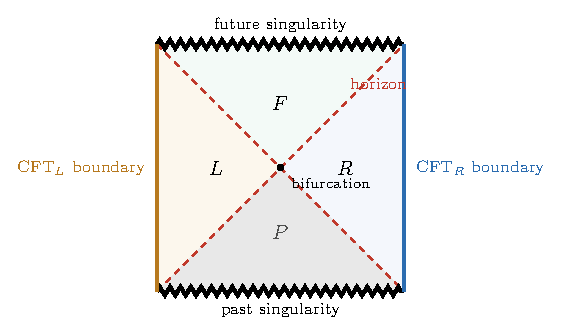
\includegraphics[width=0.72\textwidth]{figs/fig_penrose.pdf}
\caption{Penrose diagram of the two-sided eternal AdS black hole, dual to the thermofield double state $\ket{\Psi_\beta}$. The exterior regions $R$ (blue) and $L$ (gold) end on the AdS boundaries where $\mathrm{CFT}_R$ and $\mathrm{CFT}_L$ live, and are cut off from the interior regions $F$ and $P$ by the event horizons (dashed red), which cross at the bifurcation point (black dot). The wavy lines are the future and past singularities, and the gray horizontal line is the $t=0$ slice, which runs from one boundary to the other through the Einstein--Rosen bridge.}
\label{fig:penrose}
\end{figure}

\subsection*{Two puzzles, and how algebra resolves the first of them}

The $T>T_{\text{HP}}$ phase is identified with an eternal black hole, and this identification passes every
quantitative check. Even so, before the algebraic reformulation it carried two conceptual puzzles. Both are
long-standing and well known in holography.

\textbf{The factorization puzzle.} The boundary theory clearly factorizes as $\text{CFT}_R\otimes
\text{CFT}_L$. It is just two separate, non-interacting copies of the same CFT. But the bulk black hole is a
single, \emph{connected} spacetime. There are bulk operators, such as a Wilson line stretching from the left
boundary through the interior to the right boundary (Fig.~\ref{fig:penrose}), that do not seem to split into an
operator in $B(\HH_R)$ times an operator in $B(\HH_L)$. How can a connected bulk object correspond to anything
in a boundary tensor product that is clearly disconnected?

\textbf{The meeting-behind-the-horizon puzzle.} There is no interaction at all between $\text{CFT}_R$ and
$\text{CFT}_L$: the total Hamiltonian is simply $H_R+H_L$, with no cross term. Yet bulk degrees of freedom that
start separately in the $R$ and $L$ exterior regions can cross the horizon and interact with each other in the
interior. How can two boundary theories that are disconnected, both causally and dynamically, produce bulk
physics that is connected once you look behind the horizon?

The algebraic picture resolves the \emph{first} puzzle directly. Once $N\to\infty$ is taken seriously,
``$B(\HH_R)$'' is the wrong object to compare with the bulk exterior algebra. The actual large-$N$ limit of the
algebra is $Y_R$. It is type $\mathrm{III}_1$, not type I, precisely because of the order-$N^2$ entanglement
between $R$ and $L$. For a type $\mathrm{III}_1$ algebra and its commutant, there is no tensor product structure
$Y_R\otimes Y_L$ inside $B(\HH^{\text{GNS}})$ of the kind an ordinary tensor product would give. So nothing
prevents the presence of operators (such as the boundary counterpart of that Wilson line) that are not products
of an $R$-piece and an $L$-piece. The apparent contradiction came from using type I tensor-product intuition in
a regime where the algebra has already become type $\mathrm{III}_1$.

The second puzzle, meeting behind the horizon, needs more tools. It needs the emergent commutant and the
half-sided modular inclusion structure of Chapter~4. It is taken up in Chapter~8, where the bulk causal
structure of the eternal black hole is built directly from boundary algebra data.

Three further remarks prepare the ground for algebraic ER$=$EPR in Chapter~8.

First, the whole qualitative conclusion here (disconnected bulk geometry below $T_{\text{HP}}$, connected black
hole above it) could in principle have been \emph{deduced} just from watching $Y_R$ jump from type I to type
$\mathrm{III}_1$. No independent knowledge of the bulk geometry is needed.

Second, for $T>T_{\text{HP}}$ different temperatures $\beta$ lie in different, non-overlapping GNS sectors.
Their entanglement entropies differ by an amount of order $N^2$, which is an infinite barrier in the strict
limit (the mechanism of Chapter~1 again). Below $T_{\text{HP}}$, by contrast, every $\beta$ shares one common GNS
Hilbert space, and the different TFD states are just different vectors inside it.

Third, the ordinary Hamiltonians $H_R,H_L$ do not survive the large-$N$ limit as elements of the algebra. So
\eqref{eq:ads-tfd-modular} stops holding literally. But the modular operator $\Delta_\beta$ itself \emph{does}
survive, and it still generates boundary time translation in opposite directions on the two sides. Below
$T_{\text{HP}}$ it splits into an $R$ part and an $L$ part, $-\log\Delta_\beta=\beta(\hat h_R-\hat h_L)$, where
$\hat h$ is the vacuum-sector time-translation operator of the previous section. Above $T_{\text{HP}}$ it does
not split at all. This tracks the transition from type I to type $\mathrm{III}_1$ exactly.

\section{General black holes}

The thermofield double is special. It has an exact bifurcate horizon: the future and past horizons meet at a
single surface in a perfectly symmetric way. A more generic two-sided semiclassical state $\ket\Psi$ is dual to
a ``long'' black hole. Such a black hole has a genuine interior region $I$ that separates $R$ and $L$, and its
horizons do not meet at a single bifurcation surface.

This case shows the subtlety noted at the start of this chapter: the inclusion $\Sscr\subseteq\Alg_\Psi$ can
now be \emph{strict}. The renormalized single-trace algebras still reproduce the bulk exterior algebras,
$Y_R=\widetilde\M_R$ and $Y_L=\widetilde\M_L$. But $R$ and $L$ together no longer cover a full Cauchy slice. The
interior region $I$ is missing. Bulk operators in $I$ must still correspond to \emph{some} boundary operators
that survive the large-$N$ limit, since they belong to the same physical bulk field as the exterior operators,
only evaluated at a different place. But they are not single-trace operators. They must belong to
$\Alg_\Psi\setminus\Sscr$.

Chapter~7 identifies exactly what these extra operators are. They are generated from single-trace operators by
\emph{modular flow}. This mechanism was previewed by the ergodic lemma of Chapter~4: a modular flow, run long
enough, generates a whole larger algebra starting from a smaller subalgebra.

The same phenomenon (extra, non-single-trace operators needed for a black-hole interior) also occurs for a
``long'' one-sided black hole. A one-sided black hole formed by ordinary gravitational collapse, with matter
falling in from empty space, is different. This contrast matters in Chapter~7. There, $\Alg_\Psi=\Sscr$
exactly: single-trace operators are already everything, and nothing extra is needed.

\section{A diagnostic of firewalls in generic highly excited states}

Now consider a completely generic, highly excited state $\ket\Psi$ with energy $E_\Psi\sim O(N^2)$. We do not
assume that it was prepared to have a nice bulk dual. It is just an arbitrary state of that energy. The
boundary theory at such energies is expected to be chaotic. A typical state of that energy should then look
thermal to any probe made of single-trace operators, to leading order in $1/N$:
\begin{equation}
\braket{\Psi|O|\Psi}\approx\braket{O}_\beta, \qquad \braket{\Psi|O_1\cdots O_n|\Psi}\approx\braket{O_1\cdots
O_n}_\beta ,
\label{eq:ads-thermal}
\end{equation}
with $\beta$ fixed by matching the energy, $E_\Psi=E_\beta$. This is the familiar statement, in the spirit of
the eigenstate thermalization hypothesis, that a single generic high-energy state reproduces thermal
correlators. It says that, as far as single-trace operators can tell, $\Psi$ has a smooth black-hole exterior.
But does it also have a smooth \emph{interior}, a genuine continuation of the geometry behind the horizon? Or
does the interior simply fail to exist? The second possibility is called a \textbf{firewall}.

The previous section already gave the criterion needed to answer this. A smooth interior requires operators
that survive the large-$N$ limit \emph{beyond} single-trace operators, that is, $\Sscr\subsetneq\Alg_\Psi$. This
gives a clean, checkable diagnostic. \textbf{Suppose a generic highly excited state satisfies the thermal
condition \eqref{eq:ads-thermal} and \emph{also} has $\Alg_\Psi=\Sscr$, so that no operators beyond single-trace
ones survive the limit. Then its bulk dual has a firewall.} In this case $\omega_\Psi$ is a \emph{mixed} state on
$\Alg_\Psi$. This violates the purity condition \eqref{eq:ads-irreducible} assumed earlier for the ``nice''
semiclassical case.

For two-sided generic states there is an analogous statement with one more condition. The correlations between
the two sides must vanish, $\braket{\Psi|O_RO_L|\Psi}_c\to0$ as $N\to\infty$. This is consistent with there
being no smooth, connected bridge between the two boundaries in that case.

\section{Perturbative \texorpdfstring{$1/N$}{1/N} corrections}

\subsection*{Corrections to bulk reconstruction}

Everything so far worked at strictly leading order in $G_N$, or equivalently in $1/N$. Including subleading
orders makes the bulk field theory interacting: the terms $\kappa S_3+\kappa^2S_4+\cdots$ in the bulk action
switch back on. Correspondingly, the boundary theory develops nonzero connected three-point and higher
functions, suppressed by powers of $1/N$.

One direct consequence is that the HKLL formula \eqref{eq:ads-hkll}, exact at leading order, gets corrected.
Take the simplest case of a cubic self-interaction $\phi^3$ and solve the interacting bulk equation of motion
perturbatively in $\kappa$. (We do not reproduce this computation.) The result is a series of extra terms in the
bulk-to-boundary map:
\[
\begin{split}
\phi(X) ={}& \int d^dx\,K(X;x)\,O^{(0)}(x) \\
&+ \kappa\int d^dx_1\,d^dx_2\,K(X;x_1,x_2)\,O^{(0)}(x_1)O^{(0)}(x_2) + \cdots
\end{split}
\]
The leading-order reconstruction picks up multi-trace corrections, with one extra factor of a single-trace
operator for each order in $1/N$. These corrections underlie the topic of ``$1/N$ corrections to bulk
locality,'' a substantial research area of its own. We do not need to track every term here.

The structural point that matters for everything downstream is this. To any finite order in the $1/N$
expansion, the \emph{type} of each algebra discussed above is expected to stay the same as at leading order.
The heuristic reason is that the spectrum of the modular operator is controlled by its zeroth-order piece. On
this picture, perturbation theory in $1/N$ does not change an algebra's type; only the strict $N\to\infty$ limit
can do that.

\subsection*{Conserved charges, and where gravitational dressing first appears}

The second new feature matters more conceptually, for everything from Chapter~9 onward. Suppose the boundary
CFT has a global $U(1)$ symmetry. Its conserved charge must be rescaled, $\widehat Q\equiv Q/N$, in exactly the
way $\widehat H=H/N$ was, because the current itself scales as $N\Tr(\cdots)$. For a single-trace operator of
unit charge, with the convention $[Q,O(x)]=O(x)$,
\begin{equation}
[\widehat Q,O(x)]=\tfrac1N O(x) .
\label{eq:ads-charge}
\end{equation}
So the action of the rescaled charge is suppressed by $1/N$, exactly as in the time-translation story earlier
in this chapter. Within a given sector there is again a genuine large-$N$ operator $\hat q$ that generates the
full rotation, $[\hat q,O(x)]=O(x)$. Like $\hat h_\Omega$ before it, $\hat q$ cannot be written as the integral of
a local density over a single time slice.

The bulk dual of this boundary global $U(1)$ symmetry is a bulk $U(1)$ \emph{gauge} symmetry. Here something new
and physically important appears once $1/N$ corrections are included. Translate the suppressed commutator
\eqref{eq:ads-charge} to the bulk with the extrapolate dictionary. It forces the bulk gauge field strength and a
charged bulk scalar to have a \emph{nonzero commutator at spacelike separation}. This is an explicit violation of
naive bulk microcausality, order by order in $1/N$.

The violation comes directly from the bulk Gauss-law constraint. The equation of motion
$\nabla_MF^{MN}=\kappa J^N$ ties the electric field on a Cauchy slice to the charges on that same slice, because
Gauss's law is intrinsically nonlocal. The resolution comes back as the central mechanism of Chapter~9. A bulk
charged field $\phi(z,x)$ is not gauge invariant on its own. To build a gauge-invariant operator, one attaches a
\textbf{Wilson line} that runs from the boundary to the point:
\begin{equation}
\Phi(z,x) = e^{-i\kappa V}\phi(z,x), \qquad V=\int_0^z dz'\,A_z(z',x) .
\label{eq:ads-dressed}
\end{equation}
This is a \textbf{dressed observable}. The Wilson line is nonlocal: it depends on the gauge field along a whole
path, not just at one point. This nonlocality produces the nonlocal commutation relations directly, and nothing
mysterious is left over.

\subsection*{Worked calculation: Gauss's law and the dressed operator commutator}

To see this mechanism explicitly in canonical quantization, consider the bulk gauge field
$A_M = (A_t, A_z, A_x)$ on a constant-time Cauchy slice, in the gauge $A_t = 0$. We suppress the factors of the
AdS metric; they do not affect the structure of the argument. The momentum conjugate to $A_z(z,x)$ is the
electric field $E^z(z,x) = F^{zt}(z,x) = \partial_t A_z - \partial_z A_t$. The canonical commutation relation is
\[
\big[A_z(z',x'),\, F^{zt}(z'',x'')\big] = i\,\delta(z'-z'')\,\delta(x'-x'') .
\]
The field $F^{xt}$ is conjugate to $A_x$, so it commutes with $A_z$.

In the quantum theory, Gauss's law is a constraint on physical operators. Define the Gauss operator
\[
G(z'',x'') \equiv \partial_{z''} F^{zt}(z'',x'') + \partial_{x''} F^{xt}(z'',x'') - \kappa\, J^t(z'',x'') .
\]
A physical, gauge-invariant operator must commute with $G$ at every point. Take $\phi(z,x)$ to create one unit
of charge at $(z,x)$, so that $[J^t(z'',x''),\phi(z,x)]=\delta(z''-z)\,\delta(x''-x)\,\phi(z,x)$.

The naive, undressed field fails this test. It commutes with the gauge field, $[\phi(z,x), F^{Mt}] = 0$, so only
the charge term contributes:
$[G(z'',x''),\phi(z,x)]=-\kappa\,\delta(z''-z)\,\delta(x''-x)\,\phi(z,x)\ne0$. So $\phi$ is not gauge invariant.

Now compute with the dressed operator $\Phi(z,x) = e^{-i\kappa V(z,x)}\phi(z,x)$, where
$V(z,x) = \int_0^z dz' A_z(z',x)$. First, the commutator with the electric field:
\begin{align}
\big[\Phi(z,x),\, F^{zt}(z'',x'')\big]
&\eqstep{1} \Big[e^{-i\kappa \int_0^z dz' A_z(z',x)},\, F^{zt}(z'',x'')\Big]\,\phi(z,x) \notag\\
&\eqstep{2} -i\kappa \left(\int_0^z dz' \big[A_z(z',x),\, F^{zt}(z'',x'')\big]\right) \Phi(z,x) \notag\\
&\eqstep{3} -i\kappa \left(\int_0^z dz' \, i\,\delta(z'-z'')\,\delta(x-x'')\right) \Phi(z,x) \notag\\
&\eqstep{4} \kappa\,\theta(z - z'')\,\delta(x - x'')\,\Phi(z,x) . \notag
\end{align}
\stepwhy{1}{move $\phi(z,x)$ out of the commutator. It commutes with $F^{zt}$, so only the Wilson-line factor
has to be commuted.}\quad
\stepwhy{2}{$[V,F^{zt}]$ is a $c$-number, so $[e^{-i\kappa V},F^{zt}]=-i\kappa[V,F^{zt}]\,e^{-i\kappa V}$
exactly. Then recombine $e^{-i\kappa V}\phi=\Phi$.}\quad
\stepwhy{3}{substitute the canonical commutator $[A_z(z',x),F^{zt}(z'',x'')]=i\delta(z'-z'')\delta(x-x'')$.}\quad
\stepwhy{4}{$(-i)(i)=1$. The $\delta(z'-z'')$ collapses the $z'$ integral. The result is $1$ if $0<z''<z$ and $0$
if $z''>z$, which is the step function $\theta(z-z'')$.}

Next, differentiate with respect to $z''$:
\begin{align}
\partial_{z''} \big[\Phi(z,x),\, F^{zt}(z'',x'')\big]
&\eqstep{5} \kappa\, \frac{d}{dz''}\theta(z - z'')\;\delta(x - x'')\,\Phi(z,x) \notag\\
&\eqstep{6} -\kappa\,\delta(z'' - z)\,\delta(x'' - x)\,\Phi(z,x) . \notag
\end{align}
\stepwhy{5}{differentiate the result of step (4). Only the step function depends on $z''$.}\quad
\stepwhy{6}{$\frac{d}{dz''}\theta(z-z'')=-\delta(z''-z)$, the derivative of a step function.}

Finally, assemble the Gauss operator:
\begin{align}
[G(z'',x''),\Phi(z,x)]
&\eqstep{7} -\partial_{z''}\big[\Phi(z,x),F^{zt}(z'',x'')\big] - \kappa\big[J^t(z'',x''),\Phi(z,x)\big] \notag\\
&\eqstep{8} \kappa\,\delta(z''-z)\,\delta(x''-x)\,\Phi(z,x) \notag\\
&\qquad - \kappa\,\delta(z''-z)\,\delta(x''-x)\,\Phi(z,x) \ =\ 0 . \notag
\end{align}
\stepwhy{7}{$[\partial F,\Phi]=-\partial[\Phi,F]$. The $F^{xt}$ term drops out because $\Phi$ contains only
$A_z$ and $\phi$, both of which commute with $F^{xt}$.}\quad
\stepwhy{8}{use step (6) for the first term. For the second, $J^t$ commutes with the gauge field, so
$[J^t,\Phi]=e^{-i\kappa V}[J^t,\phi]=\delta\,\Phi$.}

So Gauss's law holds identically as an operator statement for the dressed field. The price is visible in step
(4). For every point $z''<z$ along the string that runs from the boundary to the insertion point, the
commutator with the electric field is nonzero, even though that point is spacelike-separated from $(z,x)$. The
nonlocal string of the Wilson line is the physical cost of gauge invariance.

The same story holds for spacetime symmetries in place of an internal $U(1)$. To make a bulk operator
diffeomorphism-invariant, one must dress it to the boundary with a \emph{gravitational} Wilson line.
Equivalently, one can work in a specific gauge and solve the constraint directly, as in the Gauss-law
calculation above. This dressing produces an analogous $1/N$ correction to the rescaled Hamiltonian,
$\widehat H=\widehat H^{(0)}+\tfrac1N\hat h_\Omega+\cdots$. \textbf{This is the first appearance, in perturbation
theory, of the mechanism that Chapter~9 turns into an exact, nonperturbative construction.} Dressing an operator
gravitationally to a physical reference is what makes it a genuine, gauge-invariant, physical observable. Here
the reference is a Wilson line; in Chapter~9 it is an observer's own clock, through the crossed product of
Chapter~5. The dressing is not optional decoration. It is forced by the bulk Gauss-law constraint that any
theory with gravity or gauge fields must satisfy.

\bigskip
\noindent The large-$N$ algebraic structure of AdS/CFT is now in place: semiclassical states as GNS sectors,
single-trace algebras $Y_O$, a change of algebra type that tracks the Hawking--Page transition, and
gravitational dressing already visible in perturbation theory. Chapter~7 assembles all of this into the central
physical claim of these notes, \textbf{subregion-subalgebra duality}. This is the statement that a bulk causal
region is identical, not merely related, to a specific emergent boundary operator subalgebra.

\chapter{Subregion-subalgebra duality}

Chapters 2--6 built the tools for the idea of this chapter. The claim is simple to state, and its
consequences are large: \textbf{in the strict large-$N$ limit, an arbitrary bulk spacetime region is not
merely \emph{related to} a boundary operator subalgebra; it \emph{is} one.} This is not an approximation,
and there is no correction term to add at this order. The algebra of the bulk region and the boundary
algebra are the same mathematical object, described in two different languages.

\section{General formulation}

\subsection*{Where the identification comes from}

Chapter 6 identified two Hilbert spaces. The first is the bulk Fock space. It is built by ordinary
quantization of small fluctuations around a classical background. The second is the boundary GNS Hilbert
space. It is built, through the GNS construction, from the algebra of boundary operators that survive the
large-$N$ limit. Since these are the same Hilbert space, the algebras of all bounded operators on them are
also the same:
\begin{equation}
B(\HH_\Psi^{\text{Fock}}) = B(\HH_\Psi^{\text{GNS}}) .
\label{eq:full_algebra_identity}
\end{equation}
This equation hides a small surprise. $B(\HH_\Psi^{\text{Fock}})$ is naturally built from data on a single
bulk Cauchy slice, because canonical quantization only needs one moment of time. $B(\HH_\Psi^{\text{GNS}})$
is built from operators on the entire boundary spacetime, or, by the time-band result of Chapter 6, at least
on a finite time band. These look like objects of different sizes. They are reconciled by the fact that the
bulk has one more spatial dimension than the boundary. The data of this extra dimension, spread over one
bulk Cauchy slice, is matched by a stretch of boundary \emph{time}, not boundary space. This is a first hint
of a general phenomenon that Chapter 8 develops in full: boundary time and bulk radial position are closely
linked.

At the free (quadratic) level, different bulk fields do not interact. So both the Hilbert space and its
operator algebra split into independent tensor factors, one for each field species $i$:
$\HH_\Psi^{\text{GNS}}=\bigotimes_i\HH_{\Psi,i}^{\text{GNS}}$, with $\HH_{\Psi,i}^{\text{Fock}}=
\HH_{\Psi,i}^{\text{GNS}}$ for each field separately. Nothing conceptually new happens here. It is
bookkeeping: the identification holds field by field, not just for the whole theory at once.

\subsection*{The duality, stated precisely}

Equation \eqref{eq:full_algebra_identity} is an identity between entire operator algebras. So it must also
hold subalgebra by subalgebra. Take any open bulk subregion $b$ of a Cauchy slice. It has a bulk operator
algebra $\widetilde\M_b \subset B(\HH_\Psi^{\text{Fock}})$. (Throughout this chapter, bulk algebras carry a
tilde, to keep them visually distinct from boundary algebras.) By \eqref{eq:full_algebra_identity}, this is
also a subalgebra of $B(\HH_\Psi^{\text{GNS}})$. When we view it as a boundary algebra we call it $\M_b$:
\begin{equation}
\widetilde\M_b = \M_b .
\label{eq:subregion_subalgebra}
\end{equation}
Read this as a literal equality, not as an analogy or a matching of some properties. There is one algebra,
with two descriptions.

Chapter 4 explained how an algebra, together with a state, encodes causal structure, entanglement, and
modular flow. Since $\M_b=\widetilde\M_b$, \textbf{the boundary algebra $\M_b$ already encodes the
corresponding structure of the bulk region $b$}. For example, the modular operator of $\widetilde\M_b$
describes how $b$ is entangled with its complement. It is exactly the modular operator of $\M_b$, and that
can be computed from boundary data alone. \textbf{This is why a bulk region can be fully ``reconstructed''
from the corresponding boundary algebra.} This statement is subregion-subalgebra duality. You have already
met two special cases of it in Chapter 6. The identifications $\widetilde\M_R=Y_R$ and $\widetilde\M_L=Y_L$
of the two black-hole exteriors in the thermofield double are exactly \eqref{eq:subregion_subalgebra}, with
$b$ taken to be the whole right or the whole left exterior region.

At this order the bulk theory is effectively a free quantum field theory, and $\widetilde\M_b$ is one of its
local algebras. So $\widetilde\M_b$ has every structural property of such algebras found in Chapter 4. By
\eqref{eq:subregion_subalgebra}, the boundary algebra $\M_b$ has the same properties:
\begin{enumerate}
\item \textbf{Reeh--Schlieder}: the bulk ``vacuum'' $\ket0_{\phi_c}$ is cyclic and separating for
$\widetilde\M_b$. Chapter 6 identified this vacuum with the boundary GNS vacuum, $\ket0_{\phi_c}=\ket1_\Psi$.
So $\ket1_\Psi$ is cyclic and separating for $\M_b$ too.
\item \textbf{Causality}: $\widetilde\M_b=\widetilde\M_{\widehat b}$, where $\widehat b$ is the domain of
dependence of $b$. In words, the algebra of a region equals the algebra of its full domain of dependence
(the time-slice axiom of Chapter 4). So $\M_b$ reconstructs the whole of $\widehat b$, not only $b$ itself.
\item \textbf{Type $\mathrm{III}_1$}: every local algebra of a continuum quantum field theory is type
$\mathrm{III}_1$ (Chapter 4). So $\widetilde\M_b$ is type $\mathrm{III}_1$, and $\M_b$ must be too.
\item \textbf{Additivity} for topologically trivial regions: $\widetilde\M_{b_1\cup b_2}=\widetilde\M_{b_1}
\vee\widetilde\M_{b_2}$.
\item \textbf{Haag duality}: $\widetilde\M_{b'}=\widetilde\M_b'$, where $b'$ is the bulk causal complement of
$b$ on its Cauchy slice.
\end{enumerate}
Each of these bulk statements becomes a checkable statement about boundary algebras once it is translated
through \eqref{eq:subregion_subalgebra}. The worked examples in the rest of this chapter all come from such
translations.

\section{Entanglement wedge reconstruction, algebraically}

\subsection*{Defining the boundary algebra $X_A$ properly}

Take a boundary spatial region $A$ on a constant-time Cauchy slice. Its \textbf{Ryu--Takayanagi (RT) surface}
$\gamma_A$ is the bulk surface of minimal area anchored on $\partial A$. The bulk region $b_A$ lying between
$A$ and $\gamma_A$ is the bulk region dual to $A$. The \textbf{entanglement wedge} $\widehat b_A$ is the bulk
domain of dependence of $b_A$ (Figure~\ref{fig:rt_entanglement_wedge}). We write $X_A$ for the boundary
algebra that subregion-subalgebra duality assigns to $b_A$:
\begin{align}
X_A \equiv \M_{b_A} &\eqstep{1} \widetilde\M_{b_A} \eqstep{2} \widetilde\M_{\widehat b_A} ,
\label{eq:XA_def}
\end{align}
\stepwhy{1}{subregion-subalgebra duality \eqref{eq:subregion_subalgebra} for the region $b=b_A$.}\quad
\stepwhy{2}{the causality property: a bulk region's algebra equals that of its domain of dependence.}

So $X_A\subset B(\HH_\Psi^{\text{GNS}})$ is the boundary algebra dual to the entanglement wedge of $A$.
Entanglement wedge reconstruction is usually stated as: physics inside $\widehat b_A$ can be fully recovered
from $A$ alone. Equation \eqref{eq:XA_def} restates this as a literal identity between algebras.

\begin{figure}[htbp]
\centering
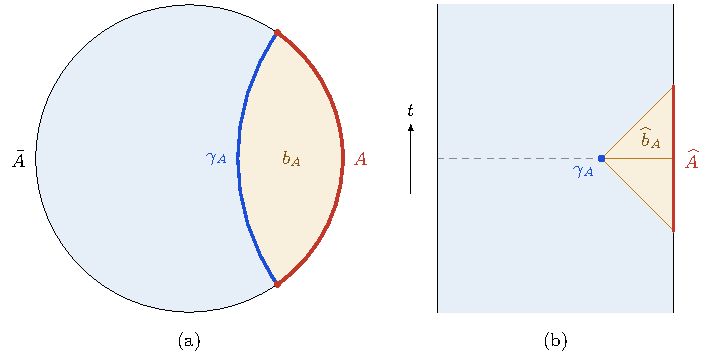
\includegraphics[width=0.82\textwidth]{figs/fig_rt.pdf}
\caption{(a) A constant-time slice of AdS drawn as a disk, whose edge is the boundary: the Ryu--Takayanagi surface $\gamma_A$ (blue) is the minimal curve anchored at the endpoints of the boundary region $A$ (red), $b_A$ (gold) is the bulk region between them, and $\bar A$ is the rest of the boundary. The entropy of $A$ is $S(A)=\mathrm{Area}(\gamma_A)/4G_N+S_{\rm bulk}(b_A)=S_{\rm gen}(b_A)$. (b) A side view, with time running upward, cut through the middle of $A$: the entanglement wedge $\widehat b_A$ (gold), bounded by light rays, is the domain of dependence of $b_A$; it meets the boundary along $\widehat A$ (red), and its tip on the $t=0$ slice (dashed) is $\gamma_A$ (blue dot).}
\label{fig:rt_entanglement_wedge}
\end{figure}

The boundary construction of $X_A$ needs some care. It is used many times below, so here it is in detail.
At finite $N$ there is an ordinary von Neumann algebra $B_A^{(N)}$ of operators localized in $A$. It
satisfies $B_A^{(N)}=B_{\widehat A}^{(N)}$, where $\widehat A$ is the boundary domain of dependence of $A$.
This is the ordinary time-slice axiom. As $N\to\infty$, many operators in $B_A^{(N)}$ have no sensible limit
and drop out. The right object is built from the operators that do survive the limit in the state $\Psi$:
\[
X_A \equiv \pi_\Psi\Big(\lim_{N\to\infty,\Psi}B_A^{(N)}\Big)'' = X_{\widehat A} .
\]
Here $\pi_\Psi$ is the GNS representation. The double commutant plays the same role as in the GNS discussion
of Chapter 2: it makes the result a genuine von Neumann algebra. The equality with $X_{\widehat A}$ holds
because the finite-$N$ time-slice axiom survives the limit. The content of entanglement wedge reconstruction
is that this boundary-defined algebra equals the bulk algebra in \eqref{eq:XA_def}.

A second algebra is easier to construct. The algebra $Y_{\widehat A}$ is generated by single-trace operators
restricted to $\widehat A$. It is the single-trace algebra $Y_O$ of Chapter 6, taken for the region
$\widehat A$. Single-trace operators in any region survive the large-$N$ limit by construction, so
\begin{equation}
Y_{\widehat A} \subseteq X_A .
\label{eq:YA_in_XA}
\end{equation}
The rest of this section studies this inclusion: what $Y_{\widehat A}$ describes in the bulk, and what else
$X_A$ contains.

\subsection*{Causal wedge reconstruction: the ``easy'' part of $X_A$}

Causal wedge reconstruction is also known as HKLL reconstruction (after Hamilton, Kabat, Lifschytz, and
Lowe). It concerns the \textbf{causal wedge}
\[
C_{\widehat A}\equiv \widetilde J^+(\widehat A)\cap\widetilde J^-(\widehat A) ,
\]
where $\widetilde J^\pm$ denote the bulk causal future and past. So $C_{\widehat A}$ is the set of bulk points
that can both receive signals from $\widehat A$ and send signals to $\widehat A$. Causal wedge reconstruction
states that bulk fields in $C_{\widehat A}$ can be written directly as single-trace operators smeared over
$\widehat A$:
\begin{equation}
\Phi(X) = \int d^dx\,K_A^{(C)}(X;x)\,\pi_\Psi(O(x)), \qquad X\in C_{\widehat A},\ x\in\widehat A .
\label{eq:HKLL_region}
\end{equation}
Here $K_A^{(C)}$ is an explicit kernel. In general it is a distribution rather than a smooth function. This
is the HKLL construction of Chapter 6, now applied to a general region instead of the whole boundary.
Algebraically, it says
\[
\widetilde\M_{C_{\widehat A}} = Y_{\widehat A} .
\]
For $A$ equal to a full boundary, this is the black-hole exterior identification of Chapter 6.

The causal wedge always lies inside the entanglement wedge, $C_{\widehat A}\subseteq\widehat b_A$. This is a
standard geometric fact. It says that causal reconstruction is always more conservative than
entanglement-based reconstruction. Combine this fact with the definition \eqref{eq:XA_def} and with
$\widetilde\M_{C_{\widehat A}}=Y_{\widehat A}$. The inclusion \eqref{eq:YA_in_XA} then follows at once: it is
the algebraic image of the geometric inclusion $C_{\widehat A}\subseteq\widehat b_A$.

\subsection*{Where the rest of $X_A$ comes from: modular flow, made explicit}

The double-commutant definition fixes $X_A$ abstractly. It does not say which operators $X_A$ contains
beyond $Y_{\widehat A}$. On the gravity side, the entanglement wedge is generically strictly larger than the
causal wedge. Equality holds only in special, highly symmetric cases. So generically
$Y_{\widehat A}\subsetneq X_A$.

Here the ergodic lemma of Chapter 4 does real work. The lemma concerns two von Neumann algebras
$\N\subset\mathcal X$ and a vector that is cyclic and separating for both. It says that the modular flow of
the larger algebra $\mathcal X$, applied to the smaller algebra $\N$, generates all of $\mathcal X$.

We apply it with $\mathcal X=X_A$. Since $b_A$ is a genuine bulk local region, $\ket1_\Psi$ is cyclic and
separating for $X_A=\widetilde\M_{b_A}$. Call the corresponding modular operator $\Delta_{X_A}$. By
\eqref{eq:subregion_subalgebra}, it equals the bulk modular operator $\widetilde\Delta_{b_A}$. For the smaller
algebra we take $Y_A^\epsilon$. This is the algebra of single-trace operators smeared within a thin time band
of width $\epsilon$ around $A$. Picture a thin strip of boundary spacetime hugging the region $A$. Its causal
wedge is a thin open bulk region next to $A$, so by the Reeh--Schlieder property $\ket1_\Psi$ is still cyclic
and separating for $Y_A^\epsilon$. The lemma then says that modular flow of the \emph{full} algebra $X_A$
regenerates all of $X_A$ from this thin sliver:
\[
X_A = \Big\{\, \Delta_{X_A}^{-is}\,O_\epsilon(\vec x)\,\Delta_{X_A}^{is} \ :\ \vec x\in A,\ s\in\mathbb R
\,\Big\}'' .
\]
Here $O_\epsilon(\vec x)$ is a single-trace operator smeared over the thin band near the point $\vec x$.
\textbf{The extra operators in $X_A$, beyond single-trace operators smeared over $\widehat A$, are
single-trace operators carried along by modular flow.}

Write $O(s;\vec x)\equiv\Delta_{X_A}^{-is}\,O_\epsilon(\vec x)\,\Delta_{X_A}^{is}$ for these modular-flowed
operators. At the free-field level of the large-$N$ limit the state is Gaussian. The modular flow of a
Gaussian state maps each smeared field to another field that is again linear in the original fields. A bulk
field is itself linear in the fields. So a bulk field anywhere in the entanglement wedge, not only in the
causal wedge, can be written as
\[
\Phi(X) = \int_{-\infty}^\infty ds\int d\vec x\,K_A^{(E)}(X;s,\vec x)\,O(s;\vec x), \qquad X\in\widehat b_A .
\]
This is the entanglement-wedge generalization of the HKLL formula \eqref{eq:HKLL_region}. Formulas of this
type were first proposed on other grounds. Here their existence follows directly from modular theory. The
kernel $K_A^{(E)}$ is in general not known in closed form.

A related result, the \textbf{JLMS relation} (Jafferis, Lewkowycz, Maldacena, and Suh, 2015), connects
boundary and bulk modular flow at large but finite $N$. In the strict large-$N$ limit it reduces to the
statement $\Delta_{X_A}=\widetilde\Delta_{b_A}$ used above. The JLMS relation is often quoted without
derivation. The box below shows how it fits together with two other holographic results.

\begin{keyresult}[: The JLMS relation and modular flow]
\textbf{Statement (JLMS).} Let $A$ be a boundary spatial region, with entanglement wedge $b_A$ bounded by the
RT surface $\gamma_A$. Work on the code subspace, the space of semiclassical states around a fixed
background. Let $\sigma$ be a reference state in it, and write the modular Hamiltonians with density matrices
(at large but finite $N$, with a short-distance cutoff where needed):
\[
H_A \equiv -\log\sigma_A , \qquad H_{\text{bulk}} \equiv -\log\sigma_{b_A} .
\]
\begin{enumerate}
\item The boundary and bulk modular Hamiltonians obey an operator identity on the code subspace,
\[
H_A = \frac{\hat A[\gamma_A]}{4G_N} + H_{\text{bulk}} + \mathcal{O}(G_N) ,
\]
where $\hat A[\gamma_A]$ is the area operator of the RT surface. (The area term is understood to include the
local terms on $\gamma_A$, such as counterterms, that also appear in the FLM formula below.)
\item For any bulk operator $\Phi \in \widetilde\M_{b_A}$ in the entanglement wedge,
\[
\Delta_A^{-is}\,\Phi\,\Delta_A^{is} = \widetilde\Delta_{b_A}^{-is}\,\Phi\,\widetilde\Delta_{b_A}^{is} .
\]
In words, boundary modular flow acts on every entanglement-wedge operator exactly as bulk modular flow does.
\end{enumerate}

\textbf{How the pieces fit.} The argument below takes two inputs: the equality of bulk and boundary relative
entropies (step 1), and the FLM formula (step 3). JLMS originally argued in the other direction. They started
from FLM, derived the modular Hamiltonian identity, and then obtained the equality of relative entropies.
Given FLM, the two statements are equivalent at this order. So the argument shows how the pieces fit
together. It is not a derivation from first principles.
\begin{enumerate}[leftmargin=*]
\item \textbf{Relative entropy equality.}
Let $\sigma$ be a reference background state, such as the global vacuum or the thermofield double. Let $\rho$
be any nearby excited state in the code subspace. The input is that the relative entropy of the boundary
region $A$ equals that of the bulk entanglement wedge $b_A$, up to small corrections:
\[
D(\rho_A \| \sigma_A) = D(\rho_{\text{bulk}} \| \sigma_{\text{bulk}}) + \mathcal{O}(G_N) .
\]

\item \textbf{Relative entropy in terms of modular Hamiltonians.}
For any two density matrices, with $H^\sigma\equiv-\log\sigma$,
\begin{align}
D(\rho\|\sigma) &\eqstep{1} \Tr(\rho\log\rho) - \Tr(\rho\log\sigma) \notag\\
&\eqstep{2} -S(\rho) + \Braket{H^\sigma}_\rho . \notag
\end{align}
\stepwhy{1}{the definition of relative entropy.}\quad
\stepwhy{2}{$S(\rho)=-\Tr(\rho\log\rho)$, and $-\log\sigma=H^\sigma$.}

Applied to the boundary state and to the bulk state in the entanglement wedge, this gives
\begin{align*}
D(\rho_A \| \sigma_A) &= -S(\rho_A) + \Braket{H_A}_\rho , \\
D(\rho_{\text{bulk}} \| \sigma_{\text{bulk}}) &= -S(\rho_{\text{bulk}}) + \Braket{H_{\text{bulk}}}_\rho .
\end{align*}

\item \textbf{The FLM formula.}
The Faulkner--Lewkowycz--Maldacena (FLM) formula is the quantum-corrected RT formula. It says that the
boundary entanglement entropy equals the bulk generalized entropy, at leading and first subleading order:
\[
S(\rho_A) = \Braket{\frac{\hat A[\gamma_A]}{4G_N}}_\rho + S(\rho_{\text{bulk}}) + \mathcal{O}(G_N) .
\]

\item \textbf{Cancellation of the bulk entropy.}
Start from the boundary relative entropy and use steps 2, 3, and 1 in turn:
\begin{align}
D(\rho_A \| \sigma_A)
&\eqstep{1} -S(\rho_A) + \Braket{H_A}_\rho \notag\\
&\eqstep{2} -\Braket{\frac{\hat A[\gamma_A]}{4G_N}}_\rho - S(\rho_{\text{bulk}}) + \Braket{H_A}_\rho
  + \mathcal O(G_N) \notag\\
&\eqstep{3} -S(\rho_{\text{bulk}}) + \Braket{H_{\text{bulk}}}_\rho + \mathcal O(G_N) . \notag
\end{align}
\stepwhy{1}{step 2 applied to the boundary state.}\quad
\stepwhy{2}{insert the FLM formula of step 3 for $S(\rho_A)$.}\quad
\stepwhy{3}{the relative entropy equality of step 1, with the bulk relative entropy written out using
step 2.}

The bulk entropy $S(\rho_{\text{bulk}})$ appears on both sides of the last equality, so it cancels.
Rearranging what is left gives
\[
\Braket{H_A}_\rho = \Braket{\frac{\hat A[\gamma_A]}{4G_N} + H_{\text{bulk}}}_\rho + \mathcal O(G_N) .
\]

\item \textbf{From expectation values to an operator identity.}
This equality holds for \emph{every} state $\rho$ in the code subspace. The expectation values of a Hermitian
operator in all density matrices supported on a subspace determine that operator's restriction to the
subspace. So the two operators agree on the code subspace:
\[
H_A = \frac{\hat A[\gamma_A]}{4G_N} + H_{\text{bulk}} + \mathcal{O}(G_N) .
\]

\item \textbf{Action on bulk operators.}
Let $\Phi \in \widetilde\M_{b_A}$ be an operator localized in the interior of the entanglement wedge. The RT
surface $\gamma_A = \partial b_A$ is the edge of the wedge, so it is spacelike separated from $\Phi$. At
leading order the area operator therefore commutes with $\Phi$:
\[
\left[\frac{\hat A[\gamma_A]}{4G_N}, \, \Phi\right] = 0 .
\]
Now compute the commutator of $\Phi$ with the boundary modular Hamiltonian:
\begin{align}
[H_A, \, \Phi] &\eqstep{1} \left[\frac{\hat A[\gamma_A]}{4G_N} + H_{\text{bulk}}, \, \Phi\right]
\eqstep{2} [H_{\text{bulk}}, \, \Phi] . \notag
\end{align}
\stepwhy{1}{the operator identity of step 5, at leading order.}\quad
\stepwhy{2}{the commutator is linear, and the area term commutes with $\Phi$.}

The operator $[H_{\text{bulk}},\Phi]$ again lies in $\widetilde\M_{b_A}$, so the same step applies to it.
Hence all nested commutators agree, $[H_A,[H_A,\dots[H_A,\Phi]]]=[H_{\text{bulk}},[H_{\text{bulk}},\dots
[H_{\text{bulk}},\Phi]]]$. Summing the exponential series of nested commutators then gives, formally,
\[
e^{is H_A}\, \Phi\, e^{-is H_A} = e^{is H_{\text{bulk}}}\, \Phi\, e^{-is H_{\text{bulk}}} .
\]
Finally, the full modular operator is $\Delta_A=\sigma_A\otimes\sigma_{\bar A}^{-1}$. Its $\sigma_{\bar A}$
factor commutes with $\Phi$, so $\Delta_A^{-is}\Phi\Delta_A^{is}=\sigma_A^{-is}\Phi\sigma_A^{is}
=e^{isH_A}\Phi e^{-isH_A}$. The same holds in the bulk. Therefore
\[
\Delta_A^{-is}\,\Phi\,\Delta_A^{is} = \widetilde\Delta_{b_A}^{-is}\,\Phi\,\widetilde\Delta_{b_A}^{is} .
\qquad \blacksquare
\]
\end{enumerate}
\end{keyresult}

When is the causal-wedge piece already everything, so that $X_A=Y_{\widehat A}$? This happens exactly when the
bulk modular flow of $b_A$ acts \emph{geometrically}. That means it acts as a pointwise coordinate
transformation, like the Rindler-wedge boost of Chapter 4. A flow of this kind maps operators localized in
$\widehat A$ to operators that are still localized in $\widehat A$, so it generates nothing new. This happens
for a half-space or a spherical region in the vacuum, and for the full boundary in the thermofield double.
These are exactly the cases already worked out explicitly. In them $X_A=Y_{\widehat A}$ and
$\widehat b_A=C_{\widehat A}$ hold exactly. In general, though, modular flow is \emph{not} geometric, and the
inclusion \eqref{eq:YA_in_XA} is strict.

\begin{physconnect}[: Modular Flow and Operator Generation]
\textbf{You have already met a finite-dimensional version of this object in Chapter 4.} There, the modular
flow of a single entangled pair, $\sigma_s(A)=\rho_R^{-is}A\rho_R^{is}$, was an ordinary unitary conjugation.
You worked it out explicitly on a $4\times4$ matrix. Here the same object, the modular flow of a boundary
algebra, does something with no finite-dimensional analogue. Starting from a small algebra, it generates
operators that were not in that algebra, and in fact the whole larger algebra. This is possible only because
the algebras involved are infinite-dimensional (here, type $\mathrm{III}_1$).

In finite dimensions the ergodic lemma has no content. Suppose $\N\subset\M$ act on a finite-dimensional
Hilbert space $\HH$, and a vector $\ket\Omega$ is cyclic for $\N$ and separating for $\M$. Because
$\ket\Omega$ is separating for $\M$, the map $x\mapsto x\ket\Omega$ is injective on $\M$, so
$\dim\M\le\dim\HH$. Because $\ket\Omega$ is cyclic for $\N$, the vectors $x\ket\Omega$ with $x\in\N$ fill all
of $\HH$, so $\dim\N\ge\dim\HH$. Together these give $\dim\N\ge\dim\M$, and so $\N=\M$. In finite dimensions
a proper subalgebra can never share such a vector with the larger algebra. There is nothing left for
modular flow to fill in.

In infinite dimensions the situation is different. By the Reeh--Schlieder property, a small subalgebra, such
as the thin sliver above, can have the same cyclic and separating vector as the larger algebra. Modular flow
can then sweep out the entire larger algebra from the sliver. This is the ``ergodic'' lemma of Chapter 4, now
doing physical work: it builds an entire entanglement wedge, or a black-hole interior, out of a thin sliver of
boundary time. The definition of modular flow has not changed. What changed is that infinite dimensions let it
do something a finite matrix conjugation cannot.
\end{physconnect}

\subsection*{Two logically distinct sources of type $\mathrm{III}_1$}

Both $X_A$ and $Y_{\widehat A}$ are type $\mathrm{III}_1$. This property can have two different physical
origins, and it helps to keep them apart.

The first origin is the one met in Chapter 4. For a continuum quantum field theory at finite $N$, the local
algebra $B_A^{(N)}$ is already type $\mathrm{III}_1$. The cause is the infinite amount of \emph{short}-range
entanglement across the boundary $\partial A$. In the bulk, this matches the fact that the RT surface reaches
the AdS boundary, which is at infinite proper distance.

To isolate the second origin, put the boundary theory on a lattice. Then at any finite $N$ the algebra
$B_A^{(N)}$ is type I: it is an algebra of finite matrices, with minimal projections. Yet $X_A$ and
$Y_{\widehat A}$, defined through the large-$N$ limit, are \emph{still} type $\mathrm{III}_1$. So their type
$\mathrm{III}_1$ property does not come from the type of $B_A^{(N)}$ before the limit. It comes from an
infinite amount of \emph{long}-range entanglement between $A$ and its complement, which appears only in the
strict $N\to\infty$ limit. In the bulk, this matches the infinite short-range entanglement of bulk fields
across the RT surface $\gamma_A$ (or, for $Y_{\widehat A}$, across the edge $\chi_{\widehat A}$ of the causal
wedge).

So two independent mechanisms produce the same type of algebra, at two different stages of the same
construction: finite $N$, and the strict $N\to\infty$ limit.

The same picture gives an algebraic way to locate the RT surface. Near $\gamma_A$, bulk modular flow acts as a
local boost. This is the local-Rindler argument of Chapter 4, applied at the RT surface. The surface
$\gamma_A$ is the fixed (``invariant'') set of that boost. By the JLMS relation, boundary modular flow acts on
wedge operators as bulk modular flow does. So \textbf{the RT surface can be characterized, without assuming a
bulk metric, as the asymptotic fixed-point set of the boundary modular flow}. This gives an algebraic
restatement of the procedure for finding the RT surface.

\subsection*{Extended gravitational systems: algebra without any geometry to point to}

The entanglement-wedge and causal-wedge story extends beyond geometric boundary regions. Replace $A$ by
\emph{any} von Neumann subalgebra $\M$ of the boundary theory. Then define $X_\M$ by the direct analogue of the
double-commutant definition of $X_A$. This definition makes sense even when there is no bulk geometric
picture at all.

One can go further. Couple a gravitational sector $B$ (which has its own boundary dual) to an ordinary
non-gravitational sector $R$. For example, $R$ could be radiation that has already escaped to infinity. For
any subsystem $Q$ of the combined system $B\cup R$, define two algebras:
\begin{itemize}
\item the entanglement wedge algebra $X_Q\equiv\lim_{G_N\to0,\Psi}B_Q$, whether or not it has a geometric
meaning;
\item the causal wedge algebra $Y_Q$, the algebra of $Q$'s ordinary low-energy effective description.
\end{itemize}
This abstraction is exactly what the evaporating-black-hole discussion later in this chapter needs. There,
$Q$ will be the emitted Hawking radiation.

\section{Quantum informational aspects of entanglement wedge reconstruction}

\subsection*{Superadditivity, and its boundary origin}

\textbf{Entanglement wedge nesting} is a standard geometric fact, which follows from the extremality of RT
surfaces. For boundary regions $A_1\subseteq A_2$, the entanglement wedges satisfy
$\widehat b_{A_1}\subseteq\widehat b_{A_2}$. Algebraically this is just $X_{A_1}\subseteq X_{A_2}$, which
follows immediately from $A_1\subseteq A_2$ and the definition of $X_A$.

Nesting has a direct geometric consequence. For two regions $A_1,A_2$ on one Cauchy slice,
\[
b_{A_1}\cup b_{A_2} \subseteq b_{A_1\cup A_2}, \qquad b_{A_1\cap A_2}\subseteq b_{A_1}\cap b_{A_2} .
\]
This is a consequence of nesting, not an extra assumption. In words, the entanglement wedge of a union is at
least as big as the union of the entanglement wedges, and generically it is strictly bigger. This is
\textbf{superadditivity of entanglement wedges}. Two AdS$_3$ examples make it concrete: two overlapping
boundary intervals, and two disjoint intervals placed close together. In both cases the RT surface of the
union ``jumps'' and encloses visibly more bulk than the two pieces do separately. Translated through the
definition \eqref{eq:XA_def}, superadditivity becomes a statement purely about boundary algebras:
\begin{equation}
X_{A_1}\vee X_{A_2} \subseteq X_{A_1\cup A_2}, \qquad X_{A_1\cap A_2}\subseteq X_{A_1}\wedge X_{A_2} .
\label{eq:superadditivity_alg}
\end{equation}

Compare this with the additivity axiom of Chapter 4 for an ordinary relativistic quantum field theory at
finite $N$. For topologically trivial regions, that axiom says $B_{A_1}^{(N)}\vee B_{A_2}^{(N)}
=B_{A_1\cup A_2}^{(N)}$. \textbf{For the inclusions \eqref{eq:superadditivity_alg} to be strict, ordinary
additivity has to fail in the strict large-$N$ limit.} One can show that it does fail in the two AdS$_3$
examples above. The argument uses a classic result of Araki. It identifies $X_{A_1}\vee X_{A_2}$ concretely as
the algebra of single-trace operators in a specific larger causal region. That algebra is strictly smaller
than $X_{A_1\cup A_2}$. (We quote this computation without reproducing it.) \textbf{Superadditivity of
entanglement wedges is the bulk geometric image of the failure of additivity for boundary algebras in the
strict large-$N$ limit.} Algebras of local regions are then no longer ``locally generated'' in the way the
algebras of an ordinary finite-$N$ quantum field theory are.

Haag duality, by contrast, survives. Assume it holds for the bulk algebras, $\widetilde\M_{b'}=
\widetilde\M_b'$. For a pure global state, $A$ and its complement $\bar A$ share the same RT surface. So
$b_{\bar A}$ is the bulk complement $b_A'$. Then Haag duality holds in the large-$N$ limit:
\[
X_{A}' = X_{\bar A} .
\]
The single-trace algebra $Y_{\widehat A}$ behaves in the opposite way. It is additive by construction, but in
general it does \emph{not} satisfy Haag duality.

\subsection*{Quantum error correction, made precise}

Entanglement wedge reconstruction has long been interpreted in the language of quantum error correction.
All the information in $b_A$ can be recovered from boundary data on $A$ alone. So this information is
protected against ``erasing'' the complementary region $\bar A$ entirely. Superadditivity makes this more
precise and checkable.

Take an operator $\Phi(X)$ at a point $X$ in a bulk region $b$. Suppose $b$ lies in the \emph{intersection}
of the entanglement wedges of two different boundary regions $A$ and $\widetilde A$, but outside the
entanglement wedge of $A\cap\widetilde A$. Picture two overlapping boundary intervals. Their wedges overlap
in a bulk region that reaches deeper than the wedge of their small common piece. Now use the HKLL-type formula
\eqref{eq:HKLL_region}. For concreteness, take a case in the vacuum sector (GNS representation $\pi_\Omega$)
where the causal and entanglement wedges coincide for both $A$ and $\widetilde A$. Then
\begin{equation}
\Phi(X) = \pi_\Omega(O_A(X)) = \pi_\Omega(O_{\widetilde A}(X)) .
\label{eq:double_reconstruction}
\end{equation}
Here $O_A(X)$ and $O_{\widetilde A}(X)$ are two \emph{different} boundary operators. They are built from
different single-trace data, smeared over $A$ and over $\widetilde A$ respectively. Yet they coincide once
represented on the GNS Hilbert space. In fact there is an infinite family of such reconstructions, one for
every boundary region whose entanglement wedge contains $b$.

\textbf{So a bulk degree of freedom $\Phi(X)$ in $b$ cannot be assigned to any one boundary region. It is
encoded collectively and redundantly across the boundary system. This is the defining feature of a quantum
error-correcting code.} This redundancy follows from superadditivity \eqref{eq:superadditivity_alg}. It is not
an extra postulate added to the holographic dictionary.

\subsection*{Worked calculation: a three-qubit toy code}

To see this redundancy in elementary matrix algebra, we work through a small toy code with three qubits. It is
a simplified cousin of the three-qutrit code of Almheiri, Dong, and Harlow, which is the standard example. The
qubit version is not perfect, as we will see, but it already shows the key mechanism.

Let the bulk logical state be a single qubit at the center of the disk:
\[
\ket{\psi}_L = \alpha \ket{0}_L + \beta \ket{1}_L, \qquad |\alpha|^2 + |\beta|^2 = 1 .
\]
The boundary consists of three physical qubits $A, B, C$. The encoding isometry
$V: \mathbb{C}^2 \to (\mathbb{C}^2)^{\otimes 3}$ is defined by
\[
\ket{0}_L \mapsto \frac{1}{\sqrt{2}}\big(\ket{000} + \ket{111}\big), \qquad
\ket{1}_L \mapsto \frac{1}{\sqrt{2}}\big(\ket{100} + \ket{011}\big) .
\]
The four basis states that appear are distinct, so the two code states are orthonormal and $V$ is an
isometry. The encoded boundary state is
\begin{align*}
\ket{\Psi(\alpha,\beta)}
&= \frac{\alpha}{\sqrt{2}}\big(\ket{000}_{ABC} + \ket{111}_{ABC}\big) \\
&\quad + \frac{\beta}{\sqrt{2}}\big(\ket{100}_{ABC} + \ket{011}_{ABC}\big) .
\end{align*}

\textbf{A single qubit.} Compute the reduced density matrix of qubit $C$ by tracing out qubits $A$ and $B$:
\[
\rho_C = \Tr_{AB}\big(\ket{\Psi}\bra{\Psi}\big) = \sum_{a,b \in \{0,1\}} \braket{ab|\Psi}\braket{\Psi|ab} .
\]
Here $\braket{ab|\Psi}$ is a (unnormalized) state of qubit $C$. The four overlaps with the basis states of
$AB$ are
\begin{align*}
\braket{00|\Psi} &= \tfrac{\alpha}{\sqrt{2}}\ket{0}_C , &
\braket{00|\Psi}\braket{\Psi|00} &= \tfrac{|\alpha|^2}{2}\ket{0}\bra{0}_C , \\
\braket{10|\Psi} &= \tfrac{\beta}{\sqrt{2}}\ket{0}_C , &
\braket{10|\Psi}\braket{\Psi|10} &= \tfrac{|\beta|^2}{2}\ket{0}\bra{0}_C , \\
\braket{11|\Psi} &= \tfrac{\alpha}{\sqrt{2}}\ket{1}_C , &
\braket{11|\Psi}\braket{\Psi|11} &= \tfrac{|\alpha|^2}{2}\ket{1}\bra{1}_C , \\
\braket{01|\Psi} &= \tfrac{\beta}{\sqrt{2}}\ket{1}_C , &
\braket{01|\Psi}\braket{\Psi|01} &= \tfrac{|\beta|^2}{2}\ket{1}\bra{1}_C .
\end{align*}
Each $AB$ basis state picks out exactly one of the four terms of $\ket\Psi$. Summing:
\begin{align}
\rho_C &\eqstep{1} \left(\frac{|\alpha|^2 + |\beta|^2}{2}\right)\ket{0}\bra{0}_C
+ \left(\frac{|\alpha|^2 + |\beta|^2}{2}\right)\ket{1}\bra{1}_C \notag\\
&\eqstep{2} \frac{1}{2}\begin{pmatrix} 1 & 0 \\ 0 & 1 \end{pmatrix} = \frac{1}{2}\id_2 . \notag
\end{align}
\stepwhy{1}{add the four terms of the table, grouping the two that multiply $\ket0\bra0_C$ and the two that
multiply $\ket1\bra1_C$.}\quad
\stepwhy{2}{normalization of the logical state, $|\alpha|^2+|\beta|^2=1$.}

So $\rho_C$ is proportional to the identity matrix. It does not depend on the logical amplitudes $\alpha$ and
$\beta$ at all. The same four-overlap computation for qubit $B$ (now tracing out $A$ and $C$) gives the same
answer, $\rho_B=\tfrac12\id_2$. So qubit $B$ alone and qubit $C$ alone each contain \textbf{no} information
about the central bulk qubit. Qubit $A$ is different. The same computation gives
$\rho_A=\tfrac12\id_2+\Re(\alpha\beta^*)\,X_A$, which does depend on the logical state. (These three reduced
density matrices were also checked numerically.) Three qubits are too few for a code in which \emph{every}
single qubit is blind to the logical information. The perfect version of this toy code uses three qutrits
(three-level systems) instead.

\textbf{Two qubits.} Now consider reconstructing logical operators on \emph{two} qubits, a boundary subregion
of size 2.
\begin{enumerate}
\item \textbf{Logical $Z_L = \ket{0}_L\bra{0} - \ket{1}_L\bra{1}$}.
Define the boundary operator $Z_{AB} \equiv Z_A \otimes Z_B$ acting on region $AB$. Then
\begin{align}
(Z_A \otimes Z_B \otimes \id_C)\ket{0}_L &\eqstep{1} \tfrac{1}{\sqrt{2}}\big( (+1)(+1)\ket{000}
+ (-1)(-1)\ket{111}\big) \notag\\
&\eqstep{2} \ket{0}_L , \notag\\
(Z_A \otimes Z_B \otimes \id_C)\ket{1}_L &\eqstep{1} \tfrac{1}{\sqrt{2}}\big( (-1)(+1)\ket{100}
+ (+1)(-1)\ket{011}\big) \notag\\
&\eqstep{2} -\ket{1}_L . \notag
\end{align}
\stepwhy{1}{$Z$ gives $+1$ on $\ket0$ and $-1$ on $\ket1$, applied to qubits $A$ and $B$; the identity leaves
qubit $C$ alone.}\quad
\stepwhy{2}{multiply the signs and compare with the encoding of $\ket0_L$ and $\ket1_L$.}

Hence $(Z_{AB} \otimes \id_C)\ket{\psi}_L = Z_L\ket{\psi}_L$.
\item \textbf{Logical $X_L = \ket{0}_L\bra{1} + \ket{1}_L\bra{0}$}.
Define the boundary operator $X_{AB} \equiv X_A \otimes \id_B$ on region $AB$. (It acts nontrivially only on
qubit $A$.) Then
\begin{align}
(X_A \otimes \id_B \otimes \id_C)\ket{0}_L &\eqstep{1} \tfrac{1}{\sqrt{2}}\big(\ket{100} + \ket{011}\big)
\eqstep{2} \ket{1}_L , \notag\\
(X_A \otimes \id_B \otimes \id_C)\ket{1}_L &\eqstep{1} \tfrac{1}{\sqrt{2}}\big(\ket{000} + \ket{111}\big)
\eqstep{2} \ket{0}_L . \notag
\end{align}
\stepwhy{1}{$X$ flips qubit $A$, $\ket0\leftrightarrow\ket1$, and leaves $B$ and $C$ alone.}\quad
\stepwhy{2}{compare with the encoding of $\ket1_L$ and $\ket0_L$.}

Hence $(X_{AB} \otimes \id_C)\ket{\psi}_L = X_L\ket{\psi}_L$.
\end{enumerate}

The logical $X_L$ can also be reconstructed on the complementary region $BC$, as
$X_{BC} \equiv \id_A \otimes X_B \otimes X_C$:
\begin{align}
(\id_A \otimes X_B \otimes X_C)\ket{0}_L &\eqstep{1} \tfrac{1}{\sqrt{2}}\big(\ket{011} + \ket{100}\big)
\eqstep{2} \ket{1}_L , \notag\\
(\id_A \otimes X_B \otimes X_C)\ket{1}_L &\eqstep{1} \tfrac{1}{\sqrt{2}}\big(\ket{111} + \ket{000}\big)
\eqstep{2} \ket{0}_L . \notag
\end{align}
\stepwhy{1}{flip qubits $B$ and $C$ in each basis state: $\ket{000}\to\ket{011}$, $\ket{111}\to\ket{100}$,
$\ket{100}\to\ket{111}$, $\ket{011}\to\ket{000}$.}\quad
\stepwhy{2}{compare with the encoding.}

Flipping only qubit $B$ would not work: $X_B\ket0_L=\tfrac1{\sqrt2}(\ket{010}+\ket{101})$ lies outside the
code subspace. Both $X_A \otimes \id_B \otimes \id_C$ and $\id_A \otimes X_B \otimes X_C$ act on the code
subspace as the central bulk operator $\Phi(0) = X_L$. Yet they are supported on disjoint, complementary
boundary regions ($A$ versus $BC$). The same kind of redundancy holds for $Z_L$. Repeating the sign computation
above with $Z$ on qubits $A$ and $C$ shows that $Z_A\otimes\id_B\otimes Z_C$ also acts as $Z_L$. So $Z_L$ can
be built on $AB$ or on $AC$.

To summarize: each of the regions $AB$ and $AC$ reconstructs the full logical algebra (both $X_L$ and $Z_L$).
The region $BC$ does not. It reconstructs $X_L$ but not $Z_L$. The reason is that every operator on $BC$
commutes with $X_A$, which acts as $X_L$, so the logical action of any operator on $BC$ must commute with
$X_L$. (A search over all three-qubit Pauli strings confirms this list of reconstructions numerically.) In the
three-qutrit code, by contrast, any two of the three qutrits reconstruct every logical operator. Even in this
imperfect qubit version, the same logical operator lives on several different boundary regions. This is the
algebraic mechanism of holographic error correction.

One caveat about this picture. The ``bulk Hilbert space as a code subspace'' picture from quantum error
correction is literally meaningful only at finite $N$. The bulk semiclassical Hilbert space, on the other hand,
is only precisely defined at $N=\infty$. So holographic error correction is better understood as a framework
connecting the two regimes. Any finite-$N$ code is necessarily only \emph{approximately} isometric, and should
not be read as a literal, exact implementation of the holographic dictionary.

\begin{physconnect}[: Redundant Purifications and Code Subspaces]
The operator $\Phi(X)$ can be written using completely different boundary data (region $A$ or region
$\widetilde A$), while remaining, in every observable sense, the same operator. This is a large-scale version
of a fact you already know from ordinary quantum information: \textbf{purification is never unique.}

Take a single mixed qubit, $\rho=\mathrm{diag}(0.7,0.3)$. One purification uses a second qubit as the
ancilla, $\ket\Psi_1=\sqrt{0.7}\ket{00}+\sqrt{0.3}\ket{11}$. A completely different one uses, say, a 3-level
ancilla, $\ket\Psi_2=\sqrt{0.7}\ket{0}\ket{a}+\sqrt{0.3}\ket{1}\ket{b}$, for any orthonormal $\ket a,\ket b$ in
the bigger ancilla space. Trace out the ancilla in either case and you get back the same $\rho$. You can check
this directly from the definition of the partial trace: the result depends only on the Schmidt coefficients
$\sqrt{0.7},\sqrt{0.3}$, not on which ancilla states carry them. \textbf{No measurement confined to the
original qubit can tell you which purification, meaning which ancilla entangled in which way, is ``really''
on the other side.} The information is present, but it is not attached to any single, canonical description of
the environment. It is attached only to the reduced state itself.

The double reconstruction \eqref{eq:double_reconstruction} works the same way, at the scale of an entire
holographic boundary instead of one ancilla qubit. The observable content of $\Phi(X)$ on the GNS Hilbert space
is fixed. But the choice of boundary data used to build it (region $A$ or region $\widetilde A$) is as
non-unique as the choice of ancilla above. As in the qubit example, no measurement of the reconstructed
operator itself can tell you which region did the reconstructing. What is new here, with no counterpart in the
single-qubit example, is the \emph{physical} content of that redundancy. It is not just a bookkeeping fact about
how $\rho$ can be written as a partial trace. Superadditivity \eqref{eq:superadditivity_alg} ties it to real
bulk geometry. It turns ``purification is not unique'' into ``a bulk region is stored redundantly enough to
survive the erasure of a boundary subregion.'' That is the operational content of a quantum error-correcting
code.
\end{physconnect}

\section{An algebraic formulation of entanglement islands}

\subsection*{The island phenomenon, restated algebraically}

The \textbf{entanglement island} phenomenon is central to modern derivations of the Page curve for an
evaporating black hole. It says the following. After the Page time $t_P$, the black-hole interior stops being
part of the black hole's own entanglement wedge. Instead it becomes part of the entanglement wedge of the
emitted radiation $R$.

Split the full system into the black-hole boundary theory $B$ and the radiation $R$
(Figure~\ref{fig:page_curve_islands}(b)). Before $t_P$, the minimal quantum extremal surface for $B$ is empty.
So $B$'s entanglement wedge is the whole Cauchy slice: the interior $I$ and the exterior $O$ together. After
$t_P$, a new, nontrivial quantum extremal surface $\alpha$ takes over, and $B$'s entanglement wedge shrinks to
the exterior $O$ alone. Algebraically,
\[
X_B = \begin{cases} \widetilde\M_O\vee\widetilde\M_I & t<t_P , \\ \widetilde\M_O & t>t_P . \end{cases}
\]
Since $B\cup R$ is the whole system, once $\widetilde\M_I$ drops out of $X_B$ it must appear in $R$'s
description instead. We use the entanglement-wedge algebra $X_R$ and the causal-wedge algebra $Y_R$ from the
discussion of extended gravitational systems earlier in this chapter. The transfer is then stated precisely as
\[
X_R = \begin{cases} Y_R & t<t_P , \\ Y_R\vee\widetilde\M_I & t>t_P . \end{cases}
\]

\begin{figure}[htbp]
\centering
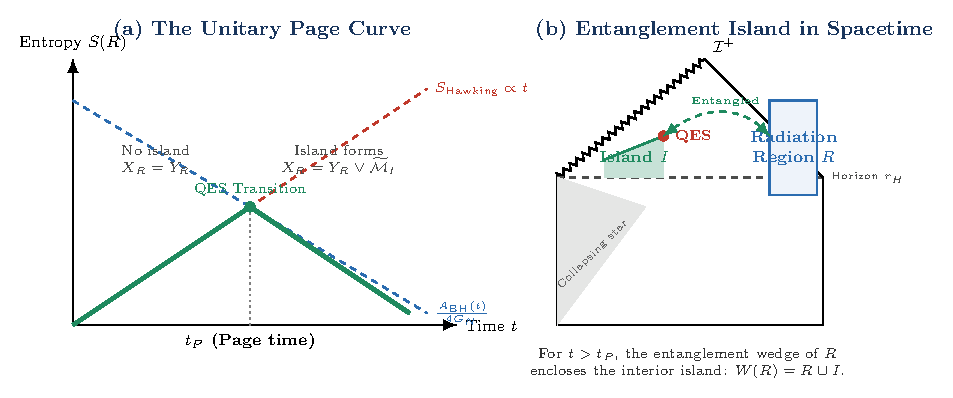
\includegraphics[width=0.95\textwidth]{figs/fig_page_curve_islands.pdf}
\caption{(a) Entropy of the radiation $R$ against time. Hawking's no-island answer (dashed red after $t_P$) keeps growing and the black hole's area term $A_{\text{BH}}/4G_N$ (dashed blue before $t_P$) keeps shrinking; the true entropy (green) follows the smaller of the two, turning over at the Page time $t_P$. (b) Penrose diagram of a black hole that forms from a collapsing star (gold) and evaporates completely, drawn after~\cite{AHMST}. The dashed red line is the event horizon and the zigzag the singularity; after the evaporation ends, the centre $r=0$ continues straight up. The dotted curve separates the region near the black hole, described by $B$, from the far region where the radiation collects (for an AdS black hole this is the boundary to which the bath is attached). On a Cauchy slice after $t_P$, the quantum extremal surface (red dot) lies just inside the horizon. The island $I$ (green) behind it joins the radiation region $R$ (blue) in the radiation's entanglement wedge, while the exterior $O$ between the red dot and the dotted curve belongs to $B$.}
\label{fig:page_curve_islands}
\end{figure}

This lets you \emph{detect} an island using only data intrinsic to the radiation system, with no reference to
$B$ at all. Define
\[
I_R \equiv Y_R'\cap X_R .
\]
These are the operators in $X_R$ that commute with every operator in $Y_R$. For $t>t_P$, this intersection is
exactly $\widetilde\M_I$. An island exists exactly when the intersection is nontrivial, that is, larger than
the multiples of the identity. In that case there are operators that survive the semiclassical limit but lie
outside $R$'s ordinary low-energy effective description. As with $X_A$ versus $Y_{\widehat A}$ above, these
extra operators are generated from $Y_R$ by the modular flow of $X_R$. It is the same mechanism once more.
The same definition, $I_Q\equiv Y_Q'\cap X_Q$, applies to any subsystem $Q$ of an extended gravitational
system, not just to radiation. An island for $Q$ is whatever survives the semiclassical limit but sits outside
$Q$'s own low-energy description.

Now return to an ordinary boundary region $A$, so that $Y_Q=Y_{\widehat A}$. Then the island algebra $I_A$
consists of the operators in $X_A$ that commute with all of $Y_{\widehat A}$. These are the operators that
modular flow adds to $Y_{\widehat A}$. Geometrically, they belong to the part of the entanglement wedge $b_A$
lying outside the causal wedge. Write $c_{\widehat A}$ for the part of $b_A$ inside the causal wedge. Then
$b_A=c_{\widehat A}\cup i_A$. This is an ordinary geometric decomposition: a causal-wedge part next to the
boundary, plus a deeper leftover piece $i_A$ between the causal wedge and the RT surface. It gives
\[
X_A=Y_{\widehat A}\vee\widetilde\M_{i_A}, \qquad I_A=\widetilde\M_{i_A} .
\]
So, in this language, an island is exactly the piece of an entanglement wedge that causal-wedge (HKLL)
reconstruction alone can never reach.

\begin{keyresult}[: Derivation of the Page Curve from the Quantum Extremal Island Rule]
\textbf{The island rule for radiation.} Consider an evaporating black hole coupled to a non-gravitational
radiation reservoir. The entropy of the radiation $R$ at boundary time $t$ is found by extremizing the
generalized entropy over candidate islands $I$, whose boundaries $\partial I$ are quantum extremal surfaces
(QES), and then taking the minimum over the extrema:
\[
S(R) = \min_{\text{QES } I} \operatorname{ext}_I \left[ \frac{\operatorname{Area}(\partial I)}{4G_N}
+ S_{\text{bulk}}(R \cup I) \right] .
\]

\textbf{The Page curve in a toy model.} The model below keeps only the features needed to see the shape of the
Page curve.
\begin{enumerate}[leftmargin=*]
\item \textbf{Evaporating black-hole geometry.}
Let the black hole form at $t = 0$ with initial horizon area $A_0$ and Bekenstein--Hawking entropy
$S_0 = A_0/4G_N$. As it radiates into the reservoir, its horizon area decreases. Let $\Gamma$ be the rate at
which its Bekenstein--Hawking entropy decreases, and take $\Gamma$ constant. (In a real evaporating black hole
the rate changes with time; a constant rate is a simplification.) Then
\[
S_{\text{BH}}(t) \equiv \frac{A_{\text{BH}}(t)}{4G_N} = S_0 - \Gamma t, \qquad t \in [0, t_{\text{evap}}] ,
\]
where $t_{\text{evap}} = S_0/\Gamma$ is the total evaporation time.

\item \textbf{Saddle 1: no island ($I = \emptyset$).}
For $I = \emptyset$ there is no boundary, $\partial I = \emptyset$, so $\operatorname{Area}(\partial I) = 0$.
The generalized entropy reduces to the bulk field-theory entropy of the radiation:
\[
S_{\text{no-island}}(R) = S_{\text{bulk}}(R) .
\]
In Hawking's semiclassical calculation, each outgoing quantum $c_k$ in the radiation is entangled with an
infalling partner mode $b_k$ behind the horizon:
\[
\ket{\text{Hawking pair}}_k \approx \frac{1}{\sqrt{2}}\big(\ket{0}_{c_k}\ket{0}_{b_k}
+ \ket{1}_{c_k}\ket{1}_{b_k}\big) .
\]
The reservoir $R$ collects only the outgoing quanta $c_k$. The partners $b_k$ stay behind the horizon. So
tracing them out leaves $R$ in a mixed state, and each new pair adds to its entropy. In the toy model we assume
that the radiation entropy grows at the same rate $\Gamma$ at which the black-hole entropy falls. (For a real
black hole the two rates differ by a factor of order one. This moves the crossing point below, but not the
shape of the curve.) Then
\[
S_{\text{no-island}}(R) = \int_0^t dt' \, \frac{dS_{\text{rad}}}{dt'} = \Gamma t .
\]
This grows without bound as $t$ increases. Eventually it exceeds the Bekenstein--Hawking entropy of the
remaining black hole. But a black hole with entropy $S_{\text{BH}}$ can be entangled with the radiation by at
most $S_{\text{BH}}$. This conflict is the \textbf{Hawking information paradox}.

\item \textbf{Saddle 2: an island ($I \ne \emptyset$).}
A second, non-empty extremum appears. Its boundary $\partial I$ is a quantum extremal surface located just
inside the event horizon. Its displacement from the horizon vanishes as $G_N\to0$. The region $I$ covers the
black-hole interior behind the horizon. The generalized entropy of this saddle is
\[
S_{\text{island}}(R) = \frac{\operatorname{Area}(\partial I)}{4G_N} + S_{\text{bulk}}(R \cup I) .
\]
Now evaluate the bulk matter entropy $S_{\text{bulk}}(R \cup I)$. The union $R \cup I$ contains \emph{both} the
outgoing Hawking quanta $c_k \in R$ \emph{and} their infalling partners $b_k \in I$. Each pair
$\ket{\text{Hawking pair}}_k$ is a pure state, so a pair lying entirely inside $R\cup I$ contributes no entropy.
The infalling and outgoing modes \textbf{purify each other}. What remains is the entropy of modes near
$\partial I$. It is of order $G_N^0$ and does not grow like $\Gamma t$:
\[
S_{\text{bulk}}(R \cup I) = \mathcal{O}(G_N^0) .
\]
So the large, steadily growing contribution is absent, and the area term dominates:
\begin{align}
S_{\text{island}}(R) &\eqstep{1} \frac{\operatorname{Area}(\partial I)}{4G_N} + \mathcal{O}(G_N^0)
\overset{(2)}{\approx} \frac{A_{\text{BH}}(t)}{4G_N} \eqstep{3} S_0 - \Gamma t . \notag
\end{align}
\stepwhy{1}{the bulk term $S_{\text{bulk}}(R\cup I)$ is only $\mathcal O(G_N^0)$, because the Hawking pairs
purify each other.}\quad
\stepwhy{2}{the quantum extremal surface sits just inside the horizon, so its area is the horizon area up to
tiny corrections, and the $\mathcal O(G_N^0)$ term is negligible next to terms of order $1/G_N$.}\quad
\stepwhy{3}{the linear decrease of the horizon area from step 1.}

\item \textbf{The Page time and the phase transition.}
By the island rule, the entropy is the smaller of the two saddle values:
\begin{align}
S(R) &\eqstep{1} \min\big\{ S_{\text{no-island}}(R), \, S_{\text{island}}(R) \big\}
\eqstep{2} \min\big\{ \Gamma t, \, S_0 - \Gamma t \big\} . \notag
\end{align}
\stepwhy{1}{the island rule: take the smallest of the extremal values.}\quad
\stepwhy{2}{substitute the two saddle values found in steps 2 and 3.}

Setting the two branches equal gives the \textbf{Page time} $t_P$:
\[
\Gamma t_P = S_0 - \Gamma t_P \implies t_P = \frac{S_0}{2\Gamma} = \frac{1}{2} t_{\text{evap}} .
\]
Over the lifetime of the black hole, the resulting entropy is
\[
S(R) = \begin{cases}
\Gamma t & t < t_P \quad (\text{no island}), \\
S_0 - \Gamma t = \frac{A_{\text{BH}}(t)}{4G_N} & t > t_P \quad (\text{island } I).
\end{cases}
\]
The early phase, with no island, is the Hawking phase. The late phase, with the interior island $I$, is the
unitary phase.
At $t = t_{\text{evap}}$, $S(R) \to 0$ as the black hole disappears. This is the value unitary evolution
requires: the final radiation is in a pure state.

\item \textbf{Algebraic translation.}
For $t < t_P$, the radiation algebra is simply $X_R = Y_R$. For $t > t_P$, the island forms, and
$X_R = Y_R \vee \widetilde\M_I$. The modular flow of $X_R$ then generates the entire interior algebra
$\widetilde\M_I$ from the radiation data alone. In this language, the resolution of the paradox needs no change
to semiclassical effective field theory. What changes at $t_P$ is which algebra the interior operators belong
to. $\blacksquare$
\end{enumerate}
\end{keyresult}

\section{Boundary description of a bulk causal diamond}

This section works through several concrete examples of the duality applied to regions that \emph{do not
touch the boundary at all}. These are purely interior bulk regions, described entirely through the commutant
structure of boundary algebras.

\subsection*{A diamond in the center of AdS, defined purely algebraically}

In the vacuum sector, take a boundary time band $I_w$ of width $w<\pi R$, where $R$ is the AdS radius. Its
causal wedge is a ``spherical Rindler region'' $W_{\rho_w}$. This is the part of global AdS outside a sphere of
radius $\rho_w=R\tan(\tfrac\pi2-\tfrac w{2R})$ around the center. It is identified with the single-trace
time-band algebra: $\widetilde\M_{W_{\rho_w}}=Y_{I_w}$. (For $w\ge\pi R$, $W_{\rho_w}$ contains an entire Cauchy
slice, and this reduces to the full-boundary statement of Chapter 6.) Now take the \emph{commutant} of both
sides, and use Haag duality, $\widetilde\M_{b'}=\widetilde\M_b'$:
\[
\widetilde\M_{D_{\rho_w}} = Y_{I_w}' .
\]
Here $D_{\rho_w}=W_{\rho_w}'$ is a spherical causal diamond centered in global AdS, as far from the boundary as
possible. \textbf{The boundary description of this diamond is not geometric at all. It is defined purely
algebraically, as the commutant of a boundary time-band algebra}, with no boundary region of its own to point
to.

As $w\to\pi R$, the time band covers nearly the whole boundary, and the causal wedge $W_{\rho_w}$ covers nearly
the whole bulk. Correspondingly, the diamond $D_{\rho_w}$ shrinks to an arbitrarily small, local patch of nearly
flat spacetime. At every stage it is described by the commutant of an ever-larger boundary time-band algebra.
This is a precise, operator-algebraic version of the holographic \textbf{IR/UV relation}: probing longer
boundary time scales (a bigger $Y_{I_w}$) is dual to probing shorter bulk distance scales (a smaller diamond
$D_{\rho_w}$).

\subsection*{Detecting a horizon from commutant structure alone}

Now repeat this in the thermofield-double black hole above the Hawking--Page temperature $T_{\text{HP}}$. Take
$Y_{I_w}^{(R)}$, the algebra of a time band of width $w$ on the right boundary. Its causal wedge is a spherical
wedge region $W_{\rho_w}$ lying strictly inside the right black-hole exterior. \emph{No matter how large $w$ is
taken}, $W_{\rho_w}$ never covers the entire $t=0$ slice of the exterior region. The horizon is what prevents
this. Algebraically,
\begin{equation}
(Y_{I_w}^{(R)})' \cap Y_R \ne \mathbb{C}\,\id, \qquad \text{for every } w .
\label{eq:horizon_commutant}
\end{equation}
Here $Y_R=\widetilde\M_R$ is the algebra of the whole right exterior, and $\mathbb C\,\id$ denotes the multiples
of the identity. \textbf{The existence of a bulk horizon is detected on the boundary by the following fact: no
matter how wide a time band you take, its commutant inside the $R$ algebra never becomes trivial.}

Compare this with the vacuum case just above. There, growing $w$ up to $\pi R$ eventually made the causal wedge
cover an entire Cauchy slice. There was no horizon, and correspondingly the commutant of the time band became
trivial once $w\ge\pi R$. Here, above the Hawking--Page transition, this never happens, for any $w$. This gives a
clean diagnostic, intrinsic to the boundary, that distinguishes a horizon-free geometry (such as empty AdS) from
a black hole. It uses nothing but the way commutants of nested time bands behave as the bands grow.

\subsection*{A single-sided collapsing black hole, and the emergence of a horizon in real time}

The richest example is a black hole formed by collapse. Take $\ket\Psi$ dual to a single-sided black hole
formed by ordinary gravitational collapse: a shell of matter falls inward from the boundary and forms a horizon
at late times. On the boundary side, this corresponds to $\ket\Psi$ thermalizing over time.

Take first an early time band $I_0$, wide enough that its causal wedge already covers a full Cauchy slice. It
gives $Y_{I_0}=B(\HH_{\text{bulk}})$, an ordinary type I algebra. No horizon has formed yet, so nothing blocks
full reconstruction. Next take, at late times well after the collapse, a semi-infinite time band $I_1$. It
reconstructs only the black-hole exterior, $\widetilde\M_R=Y_{I_1}$. Its commutant $Y_{I_1}'$ gives an emergent
``mirror'' interior algebra $\widetilde\M_L$. So a \emph{single-sided} collapse geometry reproduces the same
split structure as the two-sided eternal black hole of the thermofield double:
\[
Y_{I_0}=Y_{I_1}\vee Y_{I_1}'=\widetilde\M_R\vee\widetilde\M_L .
\]

\textbf{The type of the time-band algebra changes qualitatively as the system evolves.} It is type I at early
times, before a horizon exists. Once the system has thermalized, it is type $\mathrm{III}_1$ for a time band of
\emph{any} width, however large, as long as the band's earliest endpoint stays fixed at some late reference time.
\textbf{This change of algebra type, tracked purely from boundary data, can serve as an operator-algebraic
definition of horizon formation and thermalization in real time.} This is the idea behind the ``causal depth''
diagnostic that Chapter 8 makes precise.

\subsection*{The general theorem, and its limits}

All the examples above shared a convenient special feature. The boundary region considered was exactly the
intersection of its own causal wedge with the boundary. This fails in general: the causal wedge of a boundary
region can meet the boundary in a strictly larger region. Correspondingly, for a generic boundary region $Y$,
the naive single-trace algebra $Y_Y$ is not a von Neumann algebra on its own. Its double commutant can contain
single-trace operators supported on a region strictly larger than $Y$. This is the same phenomenon that lies
behind the failure of additivity in the superadditivity discussion earlier in this chapter.

A precise theorem, which we quote without proof, says exactly when the naive causal-wedge story works. Write
\[
C_Y\equiv (\widetilde J^+[Y]\cap\widetilde J^-[Y])''
\]
for the generalized causal wedge. Here the double prime on a set of points means its bulk causal completion
(the causal complement of the causal complement). Let $B$ denote the boundary manifold. The theorem states:
$Y_Y$ admits standard causal-wedge reconstruction, and is already a von Neumann algebra, if and only if $Y$ is
\textbf{causally convex} and $C_Y\cap B=Y$. In that case $Y_Y=\widetilde\M_{C_Y}$ exactly, with commutant
$Y_Y'=\widetilde\M_{C_Y'}$. If $Y$ fails this condition, $Y_Y''$ instead reconstructs the algebra of the larger
region $Y_{\max}\equiv C_Y\cap B$. This gives a clean, general answer to how much bigger the double commutant can
be.

\section{Generalized entropy and subregion-subalgebra duality at finite \texorpdfstring{$N$}{N}}

Everything above was stated strictly at $N=\infty$. This closing section asks what survives at finite but large
$N$. There, a bulk subregion can no longer be sharply defined, because spacetime itself fluctuates. The
section gives a significant piece of indirect evidence that the framework nonetheless extends.

Take the thermofield double above $T_{\text{HP}}$. At finite $N$, $B(\HH_R)$ is an ordinary type I algebra,
with a well-defined entanglement entropy $S_R$. At large $N$, $S_R$ should be given by the \textbf{generalized
entropy} of the dual black hole,
\begin{equation}
S_{\text{gen}} \equiv \frac{A_{\text{hor}}}{4G_N(\epsilon)} + S_{\text{bulk}}(\epsilon) .
\label{eq:Sgen_cutoff}
\end{equation}
Here $\epsilon$ is a bulk short-distance cutoff, and $G_N(\epsilon)$ is the corresponding bare Newton constant.

At strict $G_N\to0$, $\widetilde\M_R$ is type $\mathrm{III}_1$. So $S_{\text{bulk}}$ is not even defined until
$\widetilde\M_R$ is regularized into a type I algebra $\widetilde\M_R^\epsilon$ using the cutoff $\epsilon$.
The entropy of that regularized algebra has a leading UV divergence,
$S_{\text{bulk}}(\epsilon)=a\,A_{\text{hor}}/\epsilon^{d-1}+\cdots$, where $a$ is a constant that depends on
the field content and on the regulator. This is the familiar area-law divergence of Chapter 4 again. It is
matched by a divergence in the bare coupling $G_N(\epsilon)$ in the first term. Neither term in
\eqref{eq:Sgen_cutoff} is separately finite as $\epsilon\to0$. But there are strong indications, from
independent gravitational calculations, that the two divergences cancel exactly, leaving a finite
$S_{\text{gen}}=\lim_{\epsilon\to0}\big(\tfrac{A_{\text{hor}}}{4G_N(\epsilon)}+S_{\text{bulk}}(\epsilon)\big)$.

\subsection*{Worked calculation: cancellation of UV divergences in generalized entropy}

To see this cancellation explicitly, consider a free, minimally coupled scalar field in $d+1$ spacetime
dimensions. Close to a non-extremal horizon, the metric looks like Rindler space:
\[
ds^2 = -\kappa^2 \rho^2 dt^2 + d\rho^2 + dx_\perp^2 .
\]
Here $\rho$ is the proper distance to the horizon at $\rho = 0$, and $\kappa = 2\pi/\beta$ is the surface
gravity. The coordinates $x_\perp \in \mathbb{R}^{d-1}$ run along the horizon, whose total area is
$A_{\text{hor}} = \int d^{d-1}x_\perp$.

\textbf{Choice of regulator.} The coefficient of a power-law divergence depends on how the theory is
regulated. For example, a ``brick wall'' at proper distance $\epsilon$ from the horizon gives, for $d=3$, a
thermal entropy $A_{\text{hor}}/(360\pi\epsilon^2)$, while the regulator used below gives
$A_{\text{hor}}/(48\pi\epsilon^2)$. A cancellation can only be tested if both terms of \eqref{eq:Sgen_cutoff}
are regulated in the same way. We use a proper-time (heat-kernel) cutoff throughout: every heat-kernel integral
$\int ds$ is restricted to proper times $s\ge\epsilon^2$. This removes the contribution of distances shorter than
about $\epsilon$.

\textbf{Bulk entropy.} The entanglement entropy of the region outside the horizon can be computed by the replica
method. One puts the field on a cone of opening angle $2\pi\alpha$ in the $(t,\rho)$ plane (in Euclidean
signature) and uses $S=(1-\alpha\partial_\alpha)\log Z_\alpha$ at $\alpha=1$. The heat kernel on such a
two-dimensional cone contains an $s$-independent term $(1-\alpha^2)/(12\alpha)$; this is a standard result,
quoted here. The operation $(1-\alpha\partial_\alpha)$ at $\alpha=1$ turns this term into $\tfrac16$. The
transverse directions contribute a factor $A_{\text{hor}}(4\pi s)^{-(d-1)/2}$. So, with
$\log Z_\alpha=\tfrac12\int_{\epsilon^2}^\infty\frac{ds}{s}\Tr\,e^{s\Box}$,
\begin{align}
S_{\text{bulk}}(\epsilon)
&\eqstep{1} \frac12\cdot\frac16\,A_{\text{hor}}\int_{\epsilon^2}^\infty \frac{ds}{s}\,(4\pi s)^{-(d-1)/2}
  + S_{\text{bulk}}^{\text{finite}} \notag\\
&\eqstep{2} \frac{c_{d-1}\, A_{\text{hor}}}{\epsilon^{d-1}} + S_{\text{bulk}}^{\text{finite}},
\qquad c_{d-1} = \frac{1}{6(d-1)(4\pi)^{(d-1)/2}} . \notag
\end{align}
\stepwhy{1}{the replica formula applied to the cone term of the heat kernel, times the transverse factor; the
remaining, cutoff-independent part is collected in $S_{\text{bulk}}^{\text{finite}}$.}\quad
\stepwhy{2}{$\int_{\epsilon^2}^\infty ds\, s^{-(d+1)/2}=\tfrac{2}{d-1}\,\epsilon^{-(d-1)}$.}

For $d=3$ this gives $c_2=1/(48\pi)$. On its own, $S_{\text{bulk}}(\epsilon) \to +\infty$ as $\epsilon \to 0$,
as it must for a type $\mathrm{III}_1$ local algebra.

\textbf{Renormalization of Newton's constant.} Quantum fluctuations of the same scalar also correct the
gravitational effective action. In Euclidean signature, integrating out the scalar with the same cutoff gives
\[
I_{\text{eff}}[g] = -\frac{1}{16\pi G_N(\epsilon)}\int d^{d+1}x \sqrt{g}\, R + \frac{1}{2}\Tr\log(-\Box) + \dots
\]
For a minimally coupled scalar, the heat-kernel expansion is
$\Tr\,e^{s\Box}=(4\pi s)^{-(d+1)/2}\int d^{d+1}x\sqrt g\,\big(1+\tfrac{s}{6}R+\mathcal O(s^2)\big)$, and
$\tfrac12\Tr\log(-\Box)=-\tfrac12\int_{\epsilon^2}^\infty\frac{ds}{s}\Tr\,e^{s\Box}$. The term proportional to
$R$ has the same form as the Einstein--Hilbert term, so it shifts the coefficient of $\int\sqrt g\,R$:
\begin{align}
\frac{1}{16\pi G_{N,\text{ren}}}
&\eqstep{1} \frac{1}{16\pi G_N(\epsilon)} + \frac{1}{12}(4\pi)^{-(d+1)/2}
  \int_{\epsilon^2}^\infty ds\, s^{-(d+1)/2} \notag\\
&\eqstep{2} \frac{1}{16\pi G_N(\epsilon)} + \frac{c_{d-1}}{4\pi\,\epsilon^{d-1}} . \notag
\end{align}
\stepwhy{1}{collect the coefficient of $-\int\sqrt g\,R$: the bare term, plus $\tfrac12\cdot\tfrac16$ times the
proper-time integral from the $R$ term of the heat kernel.}\quad
\stepwhy{2}{do the integral as before, and use the definition of $c_{d-1}$.}

Multiplying by $4\pi$ gives
\[
\frac{1}{4G_N(\epsilon)} = \frac{1}{4G_{N,\text{ren}}} - \frac{c_{d-1}}{\epsilon^{d-1}} .
\]
For $d=3$ this is the familiar one-loop result $1/G_{N,\text{ren}}=1/G_N(\epsilon)+1/(12\pi\epsilon^2)$ for a
single scalar. (The coefficients $c_{d-1}$ in the entropy and in the coupling were also checked to agree with
a computer-algebra evaluation of the integrals, for several values of $d$.)

\textbf{The cancellation.} Now substitute this coupling into the generalized entropy $S_{\text{gen}}(\epsilon)$:
\begin{align}
S_{\text{gen}}(\epsilon) &\eqstep{1} \frac{A_{\text{hor}}}{4G_N(\epsilon)} + S_{\text{bulk}}(\epsilon) \notag\\
&\eqstep{2} \left(\frac{A_{\text{hor}}}{4G_{N,\text{ren}}} - \frac{c_{d-1}\,A_{\text{hor}}}{\epsilon^{d-1}}\right)
+ \left(\frac{c_{d-1}\,A_{\text{hor}}}{\epsilon^{d-1}} + S_{\text{bulk}}^{\text{finite}}\right) \notag\\
&\eqstep{3} \frac{A_{\text{hor}}}{4G_{N,\text{ren}}} + S_{\text{bulk}}^{\text{finite}} . \notag
\end{align}
\stepwhy{1}{the definition \eqref{eq:Sgen_cutoff} of generalized entropy with cutoff $\epsilon$.}\quad
\stepwhy{2}{insert the renormalized coupling $1/4G_N(\epsilon)=1/4G_{N,\text{ren}}-c_{d-1}/\epsilon^{d-1}$ in the
first term and the replica result for $S_{\text{bulk}}(\epsilon)$ in the second.}\quad
\stepwhy{3}{the two $c_{d-1}A_{\text{hor}}/\epsilon^{d-1}$ terms have opposite signs and cancel.}

The cutoff-dependent term $\epsilon^{-(d-1)}$ cancels exactly. Both coefficients come from the same heat-kernel
coefficient $\tfrac16$, which is why they match. So, at one loop and for this field, the generalized entropy
$S_{\text{gen}}$ does not depend on the cutoff, even though its geometric part and its field-theory part are
separately ill-defined without a regulator. For fields with non-minimal curvature couplings, or for gauge fields,
extra contributions localized on the horizon appear, and the matching needs more care. The crossed product of
Chapter 5 gives an operator-algebraic version of the same idea: it produces a type II algebra whose entropy is
finite and agrees with the generalized entropy up to a state-independent constant.

This finiteness is real, if indirect, evidence for the extension this chapter has been building toward. There
should exist a boundary regularization at finite $N$ that produces a type I algebra $Y_R^\epsilon$ with
$\widetilde\M_R^\epsilon=Y_R^\epsilon$. Nobody currently knows how to write this regularization down explicitly
for a general boundary theory. Now push $\epsilon$ down to the Planck length $\ell_p$. There, the clean separation
between the two terms of \eqref{eq:Sgen_cutoff} breaks down, since $1/G_N\sim1/\epsilon^{d-1}$. The natural
expectation is
\[
\widetilde\M_R^\epsilon = Y_R^\epsilon = B(\HH_R), \qquad \epsilon\sim\ell_p .
\]
The conjecture, then, is the following. The emergent, large-$N$, type $\mathrm{III}_1$ algebra $Y_R$ is the
strict $\epsilon\to0$ endpoint of a continuous family of type I algebras at finite $N$. This family reaches all
the way down to the ordinary finite-$N$ algebra $B(\HH_R)$ itself. In this sense subregion-subalgebra duality,
suitably reinterpreted, would survive at finite $N$, not only as a strict $N=\infty$ statement.

\bigskip
\noindent Subregion-subalgebra duality is now established as a general principle. We have worked it through for
the vacuum sector, the eternal and evaporating black holes, and purely algebraic bulk diamonds. Chapter 8 turns
to a further consequence: reading bulk \emph{causal structure itself} directly off the type and commutant
structure of boundary algebras. This includes the formation of a horizon and the connectivity of spacetime, and
no bulk metric is assumed anywhere in the argument.

\section{Sec.~VIII: Emergence of bulk geometric concepts}

Sec.~VII established that a bulk region \emph{is} a boundary algebra. This section pushes that identification
to its limit: causal structure, the formation of a horizon, and even whether two boundary theories are joined
by a wormhole at all, can each be read directly off the type and commutant structure of boundary algebras —
with no bulk metric assumed anywhere in the argument. This closes the two puzzles flagged back in Sec.~VI.C
(the factorization puzzle was already resolved there; the meeting-behind-the-horizon puzzle is resolved here,
in Sec.~VIII.B).

\subsection{Sec.~VIII.A: algebraic characterization of bulk causal structure}

\subsubsection*{Why boundary commutants can encode more than boundary causality}

Boundary operators separated in a spacelike way automatically commute — ordinary microcausality. But
\emph{timelike}-separated boundary operators are not required to commute at all; whether they do depends on
the specific representation, which is fixed by the state's two-point functions. This freedom is not a bug —
it's exactly the room needed for boundary commutant structure to encode something richer than boundary
causality alone: by subregion-subalgebra duality, it encodes bulk causal structure, in one higher dimension.

\subsubsection*{The causal depth parameter}

Recall from Sec.~VI.B (eq.~6.33) that in empty AdS, a boundary time band $I_w$ generates the entire algebra,
$Y_{I_w}=B(\HH_\Omega^{\text{GNS}})$, once $w\ge\pi R$ — geometrically, $\pi R$ is exactly the minimal width
for which light rays from the band already cover an entire bulk Cauchy slice. This motivates a purely
boundary-intrinsic definition:

\begin{quote}
\textbf{Definition (causal depth $T(t)$).} For a single-sided semiclassical state $\ket\Psi$, $T(t)$ is the
largest $w$ for which the time-band algebra $Y_{I_w(t)}$ (centered at boundary time $t$) still has a
\emph{nontrivial} commutant.
\end{quote}

For empty AdS, $T(t)=\pi R$: finite and time-independent, matching the geometric statement that light rays
from a band of exactly that width already reach everywhere. For a general horizon-free asymptotically-AdS
geometry, $T(t)$ is expected to stay finite for all time. For a single-sided eternal black hole (Fig.~26(b) of
the paper), by contrast, $Y_{I_w}$ has a \emph{nontrivial} commutant for \emph{every} finite $w$ — no matter
how wide a time band you take, you can never quite reach the full exterior algebra (only in the strict
$w\to\infty$ limit does the commutant become trivial) — so $T(t)=\infty$, for all $t$: \textbf{a purely
boundary-intrinsic signature of a horizon, requiring no bulk metric to state.} For a black hole formed by
collapse (Fig.~25 again), $T(t)$ starts finite and grows monotonically, diverging only as $t\to\infty$ — the
boundary-side signature of a horizon actually \emph{forming}, in real time, rather than always having been
there.

A two-sided version, $T_R(t)$, is defined the same way but using the \emph{relative} commutant of $Y_{I_w}$
within $Y_R$ (the right boundary's own single-trace algebra) — for the thermofield double below
$T_{\text{HP}}$, this reduces to ordinary empty AdS's $\pi R$; above $T_{\text{HP}}$, it diverges for all
time, exactly reproducing eq.~7.40's bifurcating-horizon diagnostic from Sec.~VII.E in this new language.

\begin{figure}[htbp]
\centering
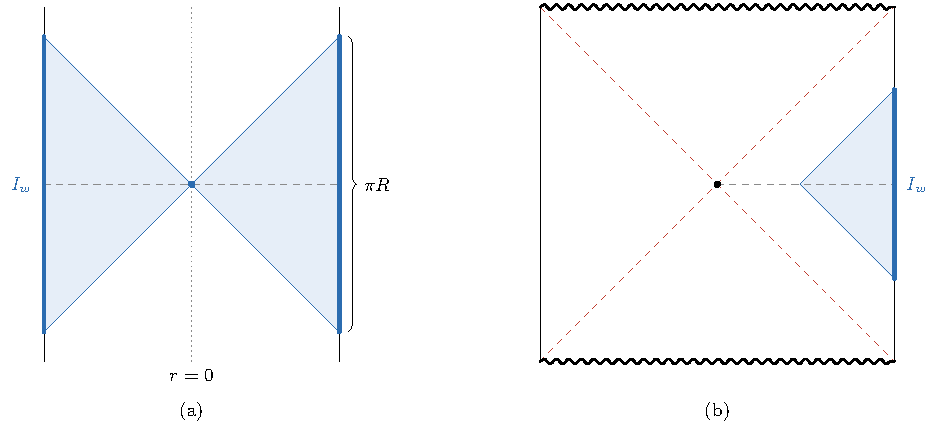
\includegraphics[width=0.90\textwidth]{figs/fig_causal_depth.pdf}
\caption{The causal depth parameter $T(t)$ as an algebraic detector of horizons. (a) In empty AdS, a boundary time band $I_w$ of width $w \ge \pi R$ sends light rays that meet at the bulk center $r=0$ and cover an entire Cauchy slice, driving the commutant to triviality ($Y_{I_w}' = \mathbb{C}\mathbf{1}$) and giving a finite causal depth $T = \pi R$. (b) In a black hole spacetime, boundary light rays asymptotically wrap around the horizon without crossing, so $Y_{I_w}' \ne \mathbb{C}\mathbf{1}$ for all finite $w$. The causal depth diverges: $T = \infty$, serving as a purely algebraic boundary diagnostic of a horizon.}
\label{fig:causal_depth}
\end{figure}

\subsubsection*{$T$ as a measure of lost determinism}

Here's a genuinely illuminating reframing of what $T$ is measuring, worth holding onto because it explains why
this whole construction is possible at all. At finite $N$, knowing the operator algebra on a single Cauchy
slice determines the whole theory (ordinary causal time evolution, the time-slice axiom of Sec.~IV.D.3). In
the strict large-$N$ limit, this stops being true — there are no equations of motion relating single-trace
operators at different times (Sec.~VI.A) — but the theory isn't completely disconnected across time either:
correlations (encoded in two-point functions) still relate a time band's algebra to the rest of the theory,
just not through equations of motion. $T$ is exactly the minimal width of a band whose algebra is
\emph{still enough}, via these correlations rather than dynamics, to recover the whole system. Read this way,
\textbf{$T=0$ is full determinism (an honest equation of motion); $T$ finite is a partial, quantifiable loss of
determinism; $T=\infty$, as in a black hole, is a complete loss of determinism — no finite window of boundary
time, however wide, is ever enough.} The emergence of the bulk radial direction is, in this precise sense,
tied to the boundary theory progressively losing determinism as $N\to\infty$.

(The paper makes this fully rigorous by relating $T$ to a classical object from harmonic analysis called the
\emph{exponential type} of the spectral function $\rho(\omega)$ — the Fourier transform of the commutator
$\braket{\Psi|[O(t),O(t')]|\Psi}$ (eqs.~8.1--8.5) — connecting it to an old question of Kolmogorov's about how
long you must observe a chaotic classical system before you can predict its entire future. This machinery is
flagged here for completeness; the physical content that matters going forward is the definition of $T$ itself
and what it measures, not the harmonic-analysis technique used to compute it in specific examples.)

\subsubsection*{Worked calculation: spectral functions and the divergence of causal depth}

To make the causal depth parameter $T(t)$ mathematically transparent, let us compute the spectral function $\rho(\omega)$ explicitly in two contrasting backgrounds: empty AdS versus a thermal black hole.
The spectral function is defined as the Fourier transform of the boundary commutator:
\[
\rho(\omega) \equiv \int_{-\infty}^\infty dt\, e^{i\omega t}\, \braket{\Psi|\big[O(t),\, O(0)\big]|\Psi}
\]
\begin{enumerate}
\item \textbf{Vacuum state $\ket\Omega$ (Empty AdS)}:
In global $\text{AdS}_{d+1}$ of radius $R$, the boundary CFT spectrum consists of discrete primaries and descendants with energies $\omega_n = (\Delta + 2n)/R$ for $n \in \mathbb{N}_0$. The Wightman function is:
\[
\braket{\Omega|O(t)O(0)|\Omega} = \sum_{n=0}^\infty c_n e^{-i(\Delta + 2n)t/R}
\]
The commutator is therefore:
\[
\braket{\Omega|\big[O(t),O(0)\big]|\Omega} = -2i \sum_{n=0}^\infty c_n \sin\big((\Delta + 2n)t/R\big)
\]
Its Fourier transform $\rho(\omega)$ is a discrete sum of delta functions:
\[
\rho(\omega) = 2\pi \sum_{n=0}^\infty c_n \Big(\delta\big(\omega - (\Delta+2n)/R\big) - \delta\big(\omega + (\Delta+2n)/R\big)\Big)
\]
Notice that $\rho(\omega) = 0$ identically in the frequency bandgap $|\omega| < \Delta/R$. By the classical Paley--Wiener theorem of Fourier analysis, a spectral function with this discrete bandgap structure has a finite exponential type:
\[
T = \pi R < \infty
\]
Thus a boundary time band of finite width $w \ge \pi R$ is sufficient to reconstruct all operators in the vacuum sector.

\item \textbf{Thermal state $\ket{\Psi_\beta}$ (BTZ Black Hole)}:
For a 2D boundary CFT at finite temperature $T = 1/\beta$, the thermal two-point function on the cylinder is:
\[
\braket{O(t)O(0)}_\beta = \left(\frac{\pi}{\beta \sinh\big(\frac{\pi}{\beta}(t - i\epsilon)\big)}\right)^{2\Delta}
\]
Taking the difference across the branch cut to evaluate the commutator and computing its Fourier transform yields:
\[
\rho(\omega) = \frac{2\pi}{\Gamma(2\Delta)}\left(\frac{2\pi}{\beta}\right)^{2\Delta - 1} \sinh\left(\frac{\beta\omega}{2}\right) \left|\Gamma\left(\Delta + \frac{i\beta\omega}{2\pi}\right)\right|^2
\]
For large frequency $|\omega| \gg 1/\beta$, Stirling's approximation gives:
\[
\rho(\omega) \approx C\, |\omega|^{2\Delta - 1} e^{-\beta |\omega| / 2}
\]
Unlike the vacuum, $\rho(\omega)$ is strictly positive and smooth for \emph{all} $\omega \in \mathbb{R}$, decaying only exponentially without any compact support or bandgap. Consequently, the exponential type of $\rho(\omega)$ is infinite:
\[
T = \infty
\]
\end{enumerate}
This provides an exact, rigorous demonstration of why the black hole horizon creates an infinite causal depth $T = \infty$: the thermal dissipation of boundary correlators completely destroys finite-time determinism.

\subsection{Sec.~VIII.B: emergence of Kruskal-like time, and resolving the meeting-behind-the-horizon puzzle}

\subsubsection*{Two kinds of bulk time}

The eternal AdS black hole geometry has two qualitatively different notions of time. \textbf{Schwarzschild
time} is an honest isometry — it maps the $R$ (or $L$) exterior region to itself, never leaving it. This is
exactly the boundary time of the thermofield double: the identification eq.~6.36 already established
Schwarzschild time as the modular time of $\widetilde\M_R=Y_R$. \textbf{Kruskal time}, by contrast, is not an
isometry at all — it's the time that actually carries a point from the exterior $R$ region across the horizon
into the interior $F$ (future) or $P$ (past) regions (Fig.~27 of the paper — the Kruskal null coordinates $U,V$
are exactly the light-cone coordinates $x^\mp$ of the Rindler-wedge discussion in Sec.~IV.E, since near the
horizon the geometry looks locally like flat Rindler space). Schwarzschild time has an obvious boundary home
(it's just ordinary boundary time evolution); Kruskal time, at first glance, has no boundary home at all —
boundary time simply runs to $\pm\infty$ as you approach the horizon and has nothing left to say about what
happens beyond it.

\subsubsection*{Kruskal time from half-sided modular inclusion}

Here is where Sec.~IV.E's half-sided modular inclusion machinery — introduced there as a purely algebraic
curiosity, worked out on an abstract Rindler-wedge light-cone example — turns out to be \emph{exactly} the
tool needed, verbatim, to manufacture Kruskal time out of nothing but boundary data. Take $\M=Y_R$ (the
right boundary's full single-trace algebra, cyclic-separating for $\ket{\Psi_\beta}$), and $\N=Y_-$, the
subalgebra generated by single-trace operators supported on the semi-infinite band $t<0$ — by Sec.~VII.E's
duality, $Y_-$ is dual to a specific bulk wedge region $W_-$ (Fig.~28 of the paper), itself type
$\mathrm{III}_1$, with $\ket{\Psi_\beta}$ cyclic and separating for it too. Because $Y_R$'s modular flow is
literally boundary time translation, $Y_-$ automatically satisfies exactly the half-sided modular inclusion
condition of eq.~4.81 — so Sec.~IV.E's machinery applies immediately, producing a genuine positive generator
$G_+\equiv\tfrac1{2\pi}(K_{Y_R}-K_{Y_-})$ (eq.~8.6), generating a brand-new time flow on $Y_R=\widetilde\M_R$
that leaves $\ket{\Psi_\beta}$ fixed. Repeating with $\N=Y_+$ (the band $t>0$) gives a second, independent
generator $G_-$.

Near the horizon — where, exactly as in Sec.~IV.E's abstract example, the geometry reduces to flat Rindler
space — these two generators act exactly as null translations in the two light-cone directions,
\[
e^{iG_+s}\phi(X)e^{-iG_+s}=\phi(X_s),\ \ X_s=(U+s,V,x_\perp)\ \ (V\ll1),
\]
\[
e^{iG_-s}\phi(X)e^{-iG_-s}=\phi(X_s),\ \ X_s=(U,V+s,x_\perp)\ \ (U\ll1)
\]
(eqs.~8.7--8.8) — \textbf{$G_\pm$, built purely from boundary modular data, literally translate a bulk operator
across the horizon}, and the combinations $p\equiv G_--G_+$, $h\equiv G_++G_-$ (eq.~8.9) generate ordinary
spatial and genuine Kruskal-time translation respectively, right in the near-horizon region.

\textbf{This resolves the meeting-behind-the-horizon puzzle from Sec.~VI.C directly}: the boundary
Hamiltonian $H=H_R+H_L$ genuinely has no term coupling $R$ to $L$ — and yet the entanglement structure of
$\ket{\Psi_\beta}$ itself, purely through the algebraic relationship between $Y_R$ and its subalgebras
$Y_\pm$, generates emergent operators $G_\pm$ that couple the two sides and translate operators from $R$ and
$L$ into causal contact behind the horizon. No interaction term was ever needed in $H$; the coupling is
already latent in how entangled the state is, made manifest only once you build the right algebraic objects
from it.

Explicit computation (worked out in detail for the BTZ black hole, not reproduced symbol-by-symbol here, but
worth knowing the shape of the answer) shows this is not just a qualitative statement — it reproduces the
\emph{exact} causal structure expected of the black hole geometry. Flowing an operator $\Phi(X,s)\equiv
e^{iG_+s}\phi(X)e^{-iG_+s}$ starting at $X=(U_0,V_0,x_\perp)$: for $s$ below a precise threshold $s_0=-U_0$,
$\Phi(X;s)$ stays entirely within $\widetilde\M_R$; the moment $s$ crosses $s_0$, operators from
$\widetilde\M_L$ suddenly, sharply appear in $\Phi(X;s)$ — exactly the moment the flowed point crosses the
horizon (Fig.~29(a)). And checking commutators directly: for two points $X_1\in R,X_2\in L$,
$[\Phi(X_1,s),\phi(X_2)]$ stays exactly zero until $s$ crosses a precise threshold $s_{12}=-U_1+U_2$, then
becomes nonzero (eq.~8.10, Fig.~29(b)) — \textbf{sharp causal structure, reproduced exactly, out of an
evolution built entirely from algebraic data with no bulk light-cone put in by hand}.

\subsubsection*{Worked derivation: Kruskal coordinates and horizon crossing in BTZ}

To see the algebra translate a point across the horizon with explicit formulas, consider the non-rotating BTZ black hole in $\text{AdS}_3$ with metric:
\[
ds^2 = -\frac{r^2 - r_+^2}{R^2} dt^2 + \frac{R^2}{r^2 - r_+^2} dr^2 + \frac{r^2}{R^2} d\phi^2
\]
The surface gravity at the horizon $r = r_+$ is $\kappa = \frac{r_+}{R^2} = \frac{2\pi}{\beta}$. Define the radial tortoise coordinate $r^*(r)$:
\[
r^*(r) \equiv \int \frac{R^2}{r^2 - r_+^2} dr = \frac{1}{2\kappa} \log\left(\frac{r - r_+}{r + r_+}\right) \in (-\infty, 0)
\]
In the right exterior wedge $R$ ($r > r_+$), define the Kruskal null coordinates:
\[
U \equiv -e^{-\kappa(t - r^*)}, \qquad V \equiv e^{\kappa(t + r^*)}
\]
Notice their properties in region $R$:
\begin{itemize}
\item $U < 0$ and $V > 0$ throughout region $R$.
\item As $r \to r_+$ ($r^* \to -\infty$), $UV = -e^{2\kappa r^*} \to 0$.
\item The future event horizon $\mathcal{H}^+$ is the null surface $U = 0$, $V > 0$.
\item The interior future region $F$ (behind the horizon) is described by $U > 0, V > 0$.
\end{itemize}
The boundary single-trace algebra $Y_R$ has modular generator $K_{Y_R} = \beta H_R = \frac{2\pi}{\kappa}(V\partial_V - U\partial_U)$, which generates Lorentz boosts in the $(U,V)$ plane leaving the horizon fixed ($U \mapsto e^{-2\pi s}U, V \mapsto e^{2\pi s}V$).

The half-sided modular translation generator $G_+ = \frac{1}{2\pi}(K_{Y_R} - K_{Y_-})$ instead acts near the horizon as a constant affine translation along the null generator:
\[
G_+ = \frac{1}{\kappa} \frac{\partial}{\partial U}
\]
Now consider an operator $\phi(U_0, V_0)$ initialized at a point $(U_0, V_0)$ in the right exterior ($U_0 < 0$). Evolving under $G_+$ for parameter $s \ge 0$:
\[
\Phi(s) \equiv e^{i G_+ s} \phi(U_0, V_0) e^{-i G_+ s} = \phi(U_0 + s,\, V_0)
\]
Let us trace the coordinate $U(s) = U_0 + s$ as the flow parameter $s$ increases:
\begin{enumerate}
\item For $0 \le s < -U_0$: $U(s) < 0$. The point remains strictly inside the right exterior wedge $R$. Therefore $\Phi(s) \in \widetilde\M_R = Y_R$.
\item At $s = s_0 \equiv -U_0$: $U(s_0) = 0$. The point hits the future horizon $\mathcal{H}^+$!
\item For $s > -U_0$: $U(s) = U_0 + s > 0$. Since $V_0 > 0$ and $U(s) > 0$, the operator has entered the **black hole interior** region $F$.
\end{enumerate}
By Haag duality and causal reconstruction, an operator at $U > 0, V > 0$ cannot commute with the left exterior algebra $\widetilde\M_L = Y_L$. For any operator $\phi(X_L)$ located at $X_L = (U_L, V_L)$ in the left wedge (where $U_L > 0, V_L < 0$), the commutator $[\Phi(s), \phi(X_L)]$ switches discontinuously from $0$ to a nonzero value at the exact threshold $s_{12} = -U_0 + U_L$.

This provides a transparent mathematical proof: the algebraic generator $G_+$, built purely from boundary modular data, translates degrees of freedom across the horizon into the interior, directly resolving the meeting-behind-the-horizon puzzle.

(In a suitable large
conformal-weight limit, this flow even becomes a genuinely \emph{local} bulk transformation, eqs.~8.11--8.12,
with trajectories running smoothly into the black hole singularity as $s$ approaches a further critical value
— and $G_\pm$ together with the boost $K$ close into an $SL(2,\mathbb R)$ algebra, exactly the 2d conformal
structure already previewed abstractly in Sec.~IV.E.) Finally, a clean consistency check: below
$T_{\text{HP}}$, $Y_R$ is type I, for which half-sided modular inclusion simply cannot occur (Sec.~IV.E's
theorem required type $\mathrm{III}_1$) — exactly matching the bulk fact that the two boundaries really are
disconnected there, with no horizon and nothing to cross.

\subsection{Sec.~VIII.C: emergent spacetime connectivity — algebraic ER\texorpdfstring{$=$}{=}EPR}

\subsubsection*{Why the naive slogan needs fixing}

The naive ER$=$EPR slogan — any two entangled gravitational systems are connected by some kind of
Einstein--Rosen bridge — runs into two genuine problems once examined carefully. \textbf{First}: below
$T_{\text{HP}}$ in the thermofield double, $R$ and $L$ are certainly entangled (an $O(G_N^0)$ amount), but the
bulk dual is two entirely \emph{disconnected} copies of AdS (Sec.~VI.C) — so ``entangled $\Rightarrow$
connected'' is already false as stated, unless you're willing to call this a ``quantum wormhole'' with no
independent definition of what that even means. \textbf{Second}, and sharper: even refining the slogan to
require $O(1/G_N)$ (i.e., large, semiclassical) entanglement specifically doesn't survive scrutiny — in an
evaporating black hole, at a time $t<t_P$ (before the Page time) but still with $O(1/G_N)$ entanglement
between the black hole and its already-emitted, causally disconnected radiation, the two systems are
\emph{classically disconnected} despite the large entanglement. Amount of entanglement alone, at any
threshold, simply isn't the right diagnostic.

\subsubsection*{The fix: entanglement \emph{structure}, not entanglement \emph{amount}}

The resolution builds directly on everything established so far in this section: Sec.~VI.C already showed that
classical bulk connectivity (a genuine, classical Einstein--Rosen bridge) corresponds to $Y_R,Y_L$ both being
type $\mathrm{III}_1$; Sec.~VIII.B just showed that type $\mathrm{III}_1$, specifically, is what makes
half-sided modular inclusion — and hence a genuine causal connection through the horizon — possible at all.
\textbf{Algebraic ER$=$EPR} promotes this from an observation into a clean, three-way classification. For two
entangled systems $R_1,R_2$ in a pure semiclassical state, with bulk dual $W_{R_1R_2}$ (every part of it
touching some boundary), and algebras $\M_{R_1},\M_{R_2}$:
\begin{itemize}
\item $W_{R_1R_2}$ is \textbf{disconnected} $\iff$ $\M_{R_1}$ and $\M_{R_2}$ are both type I.
\item $W_{R_1R_2}$ has a \textbf{classical} wormhole $\iff$ $\M_{R_1},\M_{R_2}$ are both type $\mathrm{III}_1$
\emph{and} $W_{R_1R_2}$ is classical.
\item $W_{R_1R_2}$ has a \textbf{quantum} wormhole $\iff$ $W_{R_1R_2}$ is \textbf{quantum volatile} and
$\M_{R_1},\M_{R_2}$ are not type I.
\end{itemize}
Here \textbf{quantum volatile} means the bulk spacetime fails to be classical in the $G_N\to0$ limit even
though the limit is being taken — concretely, either diffeomorphism-invariant fluctuations fail to vanish as
$G_N\to0$, or some genuine geometric quantity (a length, an area, a volume) blows up as $O(G_N^{-a})$ instead
of staying finite. The paradigm example, worth keeping firmly in mind, is exactly the evaporating black hole
around the Page time: the interior connecting the black hole to its radiation has a \emph{proper length} that
scales as $O(1/G_N)$ — diverging as $G_N\to0$ — which is precisely why it counts as quantum volatile rather
than an ordinary classical wormhole, even though the entanglement supporting it is large.

This resolves both problems cleanly. Below $T_{\text{HP}}$, both boundary algebras are type I — algebraic
ER$=$EPR correctly reports \emph{no} wormhole of either kind, fixing the first counterexample directly.
For the evaporating black hole: before the Page time, the entanglement wedge connecting black hole and
radiation is quantum volatile (that $O(1/G_N)$ interior length), so the connection there is a \emph{quantum}
wormhole, not a classical one — the second counterexample is defused by correctly classifying it as quantum
rather than either ``no wormhole'' or ``ordinary classical wormhole.'' After the Page time, the entanglement
wedge becomes genuinely classical, connecting to the radiation by an honest classical wormhole anchored at
the quantum extremal surface. (A refinement of the causal-depth parameter from Sec.~VIII.A — a \emph{modular}
depth, built from modular rather than ordinary time bands — sharpens this even further, distinguishing the
two regimes even though the boundary algebra is type $\mathrm{III}_1$ throughout: finite before the Page time,
divergent after.)

One clarifying caveat, worth keeping: this whole classification is stated for the strict $\alpha'\to0$ (large
't~Hooft coupling) limit, where genuinely geometric concepts apply in the bulk at all. In the stringy regime —
taken up next — type $\mathrm{III}_1$ alone stops being sufficient to guarantee connectivity, and the story
needs further refinement.

\subsection{Sec.~VIII.D: stringy geometry and stringy black holes (in brief)}

Everything so far assumed the bulk is well described by ordinary Einstein gravity coupled to matter — valid
in the strict $N\to\infty$, $\lambda\to\infty$ ('t~Hooft coupling, equivalently $\alpha'\to0$) double limit. At
finite $\lambda$ (finite string tension), an infinite tower of massive stringy fields appears, and the very
notion of a sharp bulk causal region — built, throughout this section, from ordinary field-theoretic causal
wedges and RT surfaces — becomes considerably more delicate: stringy effects are famously non-local at the
string scale, so the clean dictionary between bulk causal structure and boundary commutant structure
developed above needs real modification. The paper's own treatment here (its Sec.~VIII.D.1--2) works through,
in outline, how boundary operator algebras can still be used to probe causal structure and define an
analogue of a horizon in this regime, and specifically how the half-sided-modular-inclusion mechanism behind
Kruskal time (Sec.~VIII.B) generalizes to a stringy black hole — concluding that type $\mathrm{III}_1$
structure alone is no longer sufficient for connectivity once stringy effects are included, refining the
algebraic ER$=$EPR classification of the previous subsection. This material is genuinely more exploratory and
technical than the rest of the section, and is flagged here in summary rather than walked through in full
detail, since the core conceptual arc of the paper — algebra $\to$ entanglement type $\to$ emergent spacetime
— does not depend on it; it is the frontier of the subject, not its foundation.

\bigskip
\noindent With bulk causal structure, horizon formation, and spacetime connectivity now all read directly off
boundary algebra data, Sec.~IX turns to a different kind of question: rather than analyzing an existing
holographic theory, it builds simple, fully solvable \emph{toy models} of quantum gravity directly out of
operator algebras — using the crossed product of Sec.~V, now applied not as an abstract construction but as
the literal mechanism by which a physical observer's own clock produces the Bekenstein--Hawking area term and
de~Sitter entropy.

\chapter[Algebraic approaches to quantum-gravity regimes]{Algebraic approaches to\\ quantum-gravity regimes}

Chapters~6--8 analyzed an existing structure — AdS/CFT — using the machinery built in Chapters~2--5. This
chapter does something different and, in a sense, more ambitious: it builds simple, completely solvable
\emph{toy models} of quantum gravity directly out of operator algebras, with the crossed product of Chapter~5
appearing not as an abstract mathematical device but as the literal, physical mechanism that turns a quantum
field theory's type $\mathrm{III}_1$ algebra into the finite, well-defined entropy of a black hole or of
de~Sitter space. This is the payoff the whole crossed-product construction was built for.

\section{A model of gravitational dressing from observers}

\subsection*{Setting up the constraint}

Start with an ordinary quantum field theory on Hilbert space $\HH_Q$, and let $\M$ be the algebra of some
region, $\M'$ its commutant, both type $\mathrm{III}_1$, with a cyclic-separating reference $\ket\Psi$ and
modular Hamiltonian $K$ generating the usual internal time flow on $\M$ and $\M'$ (Chapter~4).

Now attach two observers, $R$ and $L$, each with their own Hamiltonian $\hat q_R,\hat q_L$ and conjugate
clock-reading operators $\hat p_R,\hat p_L$ (with clock-reading eigenstates $\ket\tau_R,\ket\tau_L$). Demand
the \emph{whole} system — field theory plus both observers — be invariant under translations generated by
\[
H = K + \hat q_R - \hat q_L .
\]
This is a toy \textbf{Hamiltonian constraint}, built to mimic the way general relativity's own Hamiltonian
constraint works: there is no external clock, only relative readings between subsystems, exactly the way
diffeomorphism invariance in gravity means only relational data (not absolute time) is physical.

The naive way to build gauge-invariant states — projecting with $\Pi\equiv\int_{-\infty}^\infty dt\,e^{-iHt}$
— fails, because $\Pi^2\propto\Pi\int dt$ diverges: the projector is not normalizable, the same obstruction met
(and resolved) in Chapter~5. The fix is to define physical states as \emph{equivalence classes} $[\psi]$ under
$\Pi\ket{\psi_1}=\Pi\ket{\psi_2}$ (states related by the gauge flow $e^{iHt}$ count as the same physical
state), with inner product $(\psi|\phi)\equiv\braket{\psi|\Pi|\phi}$, which depends only on the equivalence
classes, as can be checked directly.

\subsection*{Gauge-fixing, and two equivalent presentations}

Any state can be gauge-fixed by pinning the $L$-observer's clock to a specific reading $\tau$: expanding a
general state in the joint clock-reading$\times$field basis, one shows explicitly that $\ket\psi\sim
\ket\tau_L\otimes\ket{\psi_\tau}_{RQ}$ for $\ket{\psi_\tau}_{RQ}\equiv{}_L\!\bra\tau\Pi\ket\psi$, and this map
from the physical (gauge-invariant) Hilbert space to $\HH_R\otimes\HH_Q$ is an honest isometry, checked
directly from the definitions. In this gauge, $\hat q_L$ is no longer an independent dynamical variable — the
constraint $H=0$ solves it as a composite operator, $\hat q_L=\hat q_R+K$. Symmetrically, gauge-fixing the
$R$-observer's clock instead gives $\hat q_R=\hat q_L-K$. These are two different, but physically equivalent,
ways of describing exactly the same gauge-invariant physics.

\subsection*{Dressed operators, and the crossed product falls out automatically}

A gauge-invariant (physical) operator must commute with $H$. Starting from $A\in\M$ (or $A'\in\M'$), the
gauge-invariant, ``dressed'' version — literally the operator $A$, tagged with the $R$-observer's clock
reading $\tau$ — is built by integrating over the gauge group,
\[
\widehat A_R(\tau) \equiv \int dt\,e^{iHt}\big(\ket\tau\!\bra\tau_R\otimes A\big)e^{-iHt}
= e^{iK\hat p_R}A(-\tau)e^{-iK\hat p_R} ,
\]
with the mirror construction $\widehat A'_L(\tau)$ for $A'\in\M'$, and by construction
$[\widehat A_R(\tau),H]=0$. The clock reading $\tau$ appearing in $\widehat A_R(\tau)$ is now a \emph{quantum
number}, not a classical coordinate: in a generic state (not an eigenstate of $\hat p_R$), it genuinely
fluctuates. \textbf{The dressed operators live in a quantum spacetime.} The algebra generated by all such
dressed operators, together with clock translations, is
\[
\widehat\M \equiv \big\{\widehat A_R = e^{iK\hat p_R}Ae^{-iK\hat p_R},\ e^{i\hat q_Rs}\ \big|\ A\in\M,\
s\in\mathbb R\big\}'' ,
\]
and this is, symbol for symbol, exactly the crossed-product algebra $\widehat\M$ constructed abstractly in
Chapter~5, with the clock $\hat q$ there identified with the $R$-observer's own Hamiltonian $\hat q_R$ here.

\subsection*{Worked derivation: solving the relational constraint and dressing operators}

To see this constraint solving and dressing algebraically, work out the quantum mechanics of the relational
Hamiltonian constraint:
\[
H = K + \hat q_R - \hat q_L = 0 .
\]
Let the observers' clock variables satisfy the canonical commutation relations $[\hat p_L, \hat q_L] = -i$ and
$[\hat p_R, \hat q_R] = -i$. In the clock-reading representation $\ket{\tau_L}$, the Hamiltonian operator acts
as a differential operator $\hat q_L = i \frac{\partial}{\partial \tau_L}$.

A physical (gauge-invariant) wavefunction $\ket{\Psi_{\text{phys}}}$ must satisfy the Wheeler--DeWitt-like
equation:
\[
H \ket{\Psi_{\text{phys}}} = 0 \implies \left(K + \hat q_R - i \frac{\partial}{\partial \tau_L}\right)
\psi(\tau_L) = 0 .
\]
Integrating this first-order differential equation immediately yields:
\[
\psi(\tau_L) = e^{-i(K + \hat q_R)\tau_L} \psi(0) .
\]
Thus the entire $\tau_L$-dependence is completely determined by the data on the initial slice $\tau_L = 0$.
Choosing the gauge $\tau_L = 0$ provides a faithful, isometric embedding of the physical Hilbert space into
$\HH_R \otimes \HH_Q$:
\[
\ket{\Psi_{\text{phys}}} \longleftrightarrow \ket{\psi(0)}_{RQ} \in \HH_R \otimes \HH_Q .
\]
In this gauge, the $L$-clock momentum is eliminated via the constraint $\hat q_L = K + \hat q_R$.

Now consider dressing an operator $A \in \M$ to make it gauge-invariant under the flow $e^{i H t}$. The
group-averaged operator is:
\[
\widehat A_R(\tau) \equiv \int_{-\infty}^\infty dt\, e^{i H t} \big(\ket\tau\!\bra\tau_R \otimes A\big)
e^{-i H t} .
\]
Evaluate it on the physical gauge slice $\tau_L = 0$:
\begin{align}
\widehat A_R(\tau)
&\eqstep{1} \int_{-\infty}^\infty dt\, e^{i(K + \hat q_R)t} \big(\ket\tau\!\bra\tau_R \otimes A\big)
e^{-i(K + \hat q_R)t} \notag\\
&\eqstep{2} \int_{-\infty}^\infty dt\, \big(\ket{\tau + t}\!\bra{\tau + t}_R\big) \otimes \big(e^{i K t} A
e^{-i K t}\big) . \notag
\end{align}
\stepwhy{1}{on the slice $\tau_L=0$ the constraint replaces $\hat q_L$ by $K+\hat q_R$, so
$e^{iHt}=e^{i(K+\hat q_R)t}e^{-i\hat q_Lt}$ reduces to $e^{i(K+\hat q_R)t}$ acting on $\HH_R\otimes\HH_Q$.}\quad
\stepwhy{2}{$K$ and $\hat q_R$ act on different factors and commute, so the exponential splits;
$e^{i\hat q_Rt}$ shifts the clock state, $e^{i\hat q_Rt}\ket\tau_R=\ket{\tau+t}_R$, while $e^{iKt}$ flows
$A$ in modular time.}

Since the clock momentum operator $\hat p_R$ is diagonal in the clock basis ($\hat p_R \ket\tau_R = \tau
\ket\tau_R$), the $t$-integral collapses once the clock reading is identified with $\hat p_R$: setting
$t = \hat p_R - \tau$ inside the integral gives the closed form
\[
\widehat A_R(\tau) = e^{i K \hat p_R} A(-\tau) e^{-i K \hat p_R} .
\]
Check directly that this dressed operator commutes with the total generator $K + \hat q_R$:
\begin{align}
\big[K + \hat q_R,\, \widehat A_R(\tau)\big]
&\eqstep{3} \big[K,\, \widehat A_R(\tau)\big] + \big[\hat q_R,\, e^{i K \hat p_R} A(-\tau) e^{-i K
\hat p_R}\big] \notag\\
&\eqstep{4} i \frac{\partial}{\partial \tau}\widehat A_R(\tau) - i \frac{\partial}{\partial
\tau}\widehat A_R(\tau) \ =\ 0 . \notag
\end{align}
\stepwhy{3}{bilinearity of the commutator over the sum $K+\hat q_R$.}\quad
\stepwhy{4}{$[K,\widehat A_R(\tau)]$ is the generator of modular flow acting on $A(-\tau)$, which is
$i\partial_\tau\widehat A_R(\tau)$; the second commutator, evaluated with $[\hat q_R, e^{\pm i K \hat p_R}] =
\mp K e^{\pm i K \hat p_R}$ (from $[\hat q_R, \hat p_R] = i$), gives the same term with the opposite sign.}

The operator $\widehat A_R(\tau)$ is genuinely gauge-invariant. The algebra generated by $\{\widehat A_R,
e^{i\hat q_R s}\}$ is identically the crossed-product algebra $\M \rtimes_\sigma \mathbb{R}$.

\textbf{Gravitational dressing to a physical observer's clock \emph{is} the crossed product by the modular
group} — not an analogy, a literal identity, checkable by comparing the two constructions gauge-fixing choice
for gauge-fixing choice: fixing the $L$-observer's clock at $\tau=0$ reproduces exactly the first presentation
of $\widehat\M$ and $\widehat\M'$ in Chapter~5; fixing the $R$-observer's instead reproduces the second
presentation, in which undressed elements of $\M$ sit directly inside $\widehat\M$. And since $K$ here is a
genuine modular Hamiltonian, the theorem of Chapter~5 applies immediately: $\widehat\M$ and $\widehat\M'$ are
type $\mathrm{II}_\infty$, with honest density operators and entropies — no further argument needed, since
it is literally the same construction already proven there.

\section{Application I: quantum volatile black hole spacetime and its entropy}

Apply the model directly to the eternal AdS black hole: $\HH_Q$ is the bulk QFT in the black-hole geometry at
$G_N\to0$, $\ket\Psi$ is the Hartle--Hawking vacuum, $\M=\widetilde\M_R$, $\M'=\widetilde\M_L$, and $K$
generates ordinary Schwarzschild time. With two genuine asymptotic boundaries available, it is natural to
identify the $R,L$ ``observers'' of the previous section with the two boundaries themselves, and
$\hat q_R,\hat q_L$ with (mean-subtracted) perturbations of the boundary Hamiltonians $H_R,H_L$ around their
background values — concretely, in a microcanonical thermofield double peaked around energy $E_0\sim O(N^2)$
with an $O(N^0)$ spread, $\hat q_R\equiv H_R-\braket{H_R}$.

The crossed-product algebras are type $\mathrm{II}_\infty$ — and this genuinely reflects a change in the
physical spacetime structure. The gauge-invariant, but now quantum, quantity $\hat p_R+\hat p_L$ (the time
separation between the $R$ and $L$ boundaries, represented geometrically by a geodesic running between them)
has $O(1)$ fluctuations as $G_N\to0$ — precisely an example of the \textbf{quantum volatile geometry} met in
Chapter~8: \textbf{the two boundaries are connected by a genuine quantum wormhole}, not a classical one.

Now the entropy payoff, which closes the loop opened at the start of Chapter~5. For a semiclassical excited
state $\ket{\widehat\Phi}=\ket\Phi\otimes\ket g$ (exactly the construction of Chapter~5), the crossed-product
entropy formula of Chapter~5 gives
\[
S_{\widehat\M_R}^{(\widehat\Phi)} = -S(\Phi\|\Psi) + \text{const} .
\]
Separately — a gravitational computation quoted here rather than re-derived — it has been shown that,
assuming the system relaxes back to the equilibrium state $\ket\Psi$ as $t\to\infty$, this same relative
entropy is exactly (minus, up to an additive constant) the ordinary generalized entropy of the excited state,
$S(\Phi\|\Psi)=-S_{\text{gen}}^{(\Phi)}+\text{const}$. Combining the two:
\[
S_{\widehat\M_R}^{(\widehat\Phi)} = S_{\text{gen}}^{(\Phi)} + \text{const} .
\]
\textbf{The type II entropy of the gravitationally dressed algebra literally \emph{is} the generalized
(Bekenstein--Hawking $+$ bulk-matter) entropy of the black hole, up to a state-independent constant.} Every
algebraic step in this chain — crossed product, type II, its entropy formula — was proved in full generality in
Chapter~5; the only new input is the quoted gravitational identity relating relative entropy to generalized
entropy.

\section{Application II: de Sitter entropy}

\subsection*{The puzzle}

De~Sitter space has no boundary at all — quantum gravity there faces a much deeper ``problem of time'' than
AdS does, with no asymptotic region to anchor observables to. A static observer (sitting at a pole of the
spatial sphere) only ever accesses a \textbf{static patch}, bounded by a cosmological horizon at the de~Sitter
radius $R$ (Fig.~\ref{fig:desitter}). The horizon carries the celebrated Gibbons--Hawking entropy,
$S_{\text{dS}}=A_{\text{hor}}^{(0)}/4G_N$ — but its physical meaning has been debated for decades (does its
exponential count a genuine, finite-dimensional de~Sitter Hilbert space, for instance?), with little concrete
progress.

\begin{figure}[htbp]
\centering
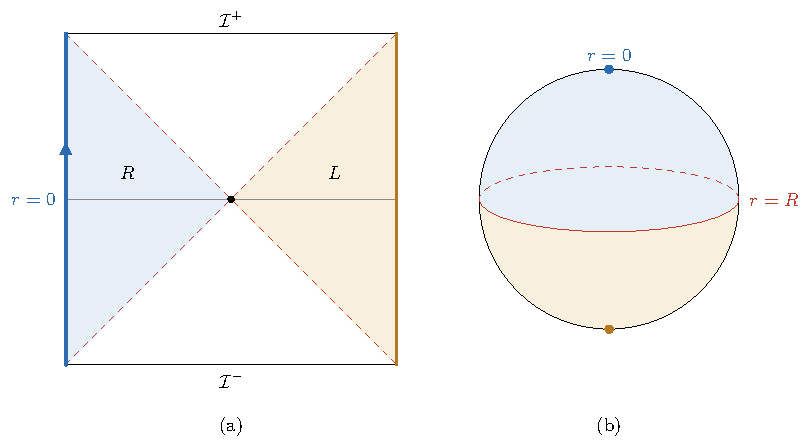
\includegraphics[width=0.82\textwidth]{figs/fig_desitter.pdf}
\caption{(a) Penrose diagram of global de~Sitter space. The left edge is the worldline of a static observer at the north pole $r=0$ (blue arrow); the cosmological horizons (dashed red diagonals) confine everything this observer can ever see to the static patch $R$ (blue), while the patch $L$ (gold) belongs to an observer at the south pole (right edge). The top and bottom edges are future and past infinity $\mathcal I^\pm$, and the gray line is the $t=0$ slice. (b) That slice is a sphere: its northern half (blue) lies in $R$ and ends on the horizon $r=R$ (red equator), which is the black dot in (a).}
\label{fig:desitter}
\end{figure}

The \emph{generalized} de~Sitter entropy, $S_{\text{gen}}=A_{\text{hor}}/4G_N+\widetilde S_R$, has a strange
feature that is the opposite of a black hole's behavior: \textbf{exciting matter in the static patch
\emph{decreases} $S_{\text{gen}}$}, because it shrinks the cosmological horizon area faster than it grows the
matter entanglement $\widetilde S_R$. This can be checked completely explicitly: put a black hole of mass
parameter $\mu$ inside the static patch (giving a black-hole horizon at $r_b$ nested inside the cosmological
horizon at $r_c>r_b$), represent $\widetilde S_R$ by the black-hole horizon area itself, and the generalized
entropy comes out to $S_{\text{gen}}=\omega_{d-2}(r_c^{d-2}+r_b^{d-2})/4G_N$, which is \emph{always less} than
$S_{\text{dS}}$ — so $S_{\text{dS}}$ is the maximum possible value of $S_{\text{gen}}$, achieved exactly by
empty de~Sitter.

\subsection*{Worked calculation: why matter excitations decrease de~Sitter entropy}

To see this thermodynamic behavior in detail, consider a four-dimensional Schwarzschild--de~Sitter spacetime
with metric:
\[
ds^2 = -f(r) dt^2 + \frac{dr^2}{f(r)} + r^2 d\Omega_2^2, \qquad f(r) = 1 - \frac{2 G_N M}{r} -
\frac{r^2}{R^2} .
\]
\begin{enumerate}
\item \textbf{Empty de~Sitter space ($M = 0$)}:
The horizon condition $f(r) = 1 - r^2/R^2 = 0$ gives a single cosmological horizon at $r_c^{(0)} = R$.
The cosmological horizon area is $A_{\text{dS}} = 4\pi R^2$, giving the Gibbons--Hawking entropy:
\[
S_{\text{dS}} = \frac{A_{\text{dS}}}{4 G_N} = \frac{\pi R^2}{G_N} .
\]
\item \textbf{Matter excitation: small black hole ($0 < G_N M \ll R$)}:
For a localized excitation of mass $M$, the horizon equation $f(r) = 0$ has two positive roots: a black hole
horizon at $r_b$ and a shifted cosmological horizon at $r_c < R$.
Let $r_c = R(1 - \delta)$ with $\delta \ll 1$. Expanding $f(r_c) = 0$ to first order in $\delta$ and $M$:
\[
1 - \frac{2 G_N M}{R} - (1 - 2\delta) \approx 0 \implies \delta = \frac{G_N M}{R} .
\]
Therefore the cosmological horizon shrinks to $r_c \approx R\left(1 - \frac{G_N M}{R}\right)$.
Its shifted area is:
\[
A_c(M) = 4\pi r_c^2 \approx 4\pi R^2 \left(1 - \frac{2 G_N M}{R}\right) = A_{\text{dS}} - 8\pi G_N M R .
\]
The black hole horizon is at $r_b \approx 2 G_N M$, with area $A_b(M) = 4\pi r_b^2 \approx 16\pi G_N^2 M^2
\sim O(G_N^2 M^2)$.
The total generalized entropy is the sum of both horizon areas:
\begin{align}
S_{\text{gen}}(M) = \frac{A_c(M)}{4 G_N} + \frac{A_b(M)}{4 G_N}
&\eqstep{1} \frac{A_{\text{dS}} - 8\pi G_N M R}{4 G_N} + O(G_N M^2) \notag\\
&\eqstep{2} S_{\text{dS}} - 2\pi M R + O(G_N M^2) . \notag
\end{align}
\stepwhy{1}{substitute the shifted cosmological area $A_c(M)=A_{\text{dS}}-8\pi G_NMR$, and note that the
black-hole term $A_b/4G_N\approx4\pi G_NM^2$ is second order in $M$.}\quad
\stepwhy{2}{split the fraction: $A_{\text{dS}}/4G_N=S_{\text{dS}}$ and $8\pi G_NMR/4G_N=2\pi MR$.}
\end{enumerate}
Here $\beta_{\text{dS}} = 2\pi R$ is the inverse Gibbons--Hawking temperature. Thus, to linear order in
perturbation:
\[
S_{\text{gen}}(M) - S_{\text{dS}} = -\beta_{\text{dS}} M < 0 \quad \text{for all } M > 0 .
\]
Any localized energy excitation inside the static patch strictly \textbf{lowers} the generalized entropy.
Consequently, empty de~Sitter ($M = 0$) is the unique state of \textbf{maximal entropy}.

\subsection*{Recognizing the type \texorpdfstring{$\mathrm{II}_1$}{II1} signature}

This behavior — a reference state whose entropy can only ever decrease under perturbation — is exactly what
appeared, worked out on an explicit example, in the type $\mathrm{II}_1$ Bell-pair chain of Chapter~3, where
perturbing away from the maximally entangled $\ket{\Phi_{\pi/4}}$ always gives $S_\M(\Psi)\le0$.
\textbf{Empty de~Sitter behaves exactly like the maximally entangled reference state of a type
$\mathrm{II}_1$ algebra, with $R$ and $L$ static patches playing the role of the two entangled halves.}

Making this precise uses exactly the observer model above, with one small but crucial modification. Take
$\HH_Q$ to be the QFT Hilbert space on global de~Sitter, $\ket\Psi$ the Bunch--Davies vacuum, $\M,\M'$ the $R$-
and $L$-patch algebras (modular Hamiltonian $K$ = the boost generator of $t$-translations), and $\hat q_R,\hat
q_L$ the Hamiltonians of static observers at the two poles. This reproduces $\widehat\M_R,\widehat\M_L$ exactly
as before — \emph{except} that now $\hat q_R,\hat q_L$ are required to be \textbf{bounded below} (non-negative
eigenvalues — physically, the sensible statement that a real observer's energy cannot be negative). By exactly
the mechanism checked in Chapter~5 (restricting the clock spectrum to $q\ge0$ turns a divergent trace into a
normalized one), $\widehat\M_R,\widehat\M_L$ become type $\mathrm{II}_1$, not type $\mathrm{II}_\infty$. The
type $\mathrm{II}_1$ entropy relative to the maximally entangled reference state
$\ket{\widehat\Psi_T}=e^{-\hat q/2}\otimes\ket0_{\text{BD}}$, with trace $\tr(\cdots)\equiv\braket{
\widehat\Psi_T|\cdots|\widehat\Psi_T}$, is negative exactly the way the Chapter~3 example was, and for the
identical reason: there is no unentangled reference to fall below zero from, only a maximally entangled one to
fall below.

One more consistency check resolves an objection that looks fatal at first glance: if empty de~Sitter is a
maximally entangled state, should it not have infinite temperature (the way a maximally entangled Bell pair
has infinite temperature in the entanglement-Hamiltonian sense)? The resolution: the state
$\ket{\widehat\Psi_T}$ has density operator $\rho=e^{-K}$ on the crossed-product algebra — a thermal state at
\emph{dimensionless} temperature exactly $1$, the universal modular temperature of Tomita--Takesaki theory
(Chapter~4). Converting this dimensionless $\beta=1$ into physical units using the static observer's own
proper time $t$ reproduces exactly the known, finite de~Sitter temperature $T_{\text{dS}}=1/2\pi R$. There is
no contradiction: ``maximally entangled'' was always a dimensionless, modular-time statement, and the finite
physical temperature only appears once you convert to an observer's physical clock.

\begin{table}[htbp]
\centering
\small
\renewcommand{\arraystretch}{1.3}
\begin{tabularx}{\textwidth}{>{\bfseries\color{navyhead}}l >{\raggedright\arraybackslash}X >{\raggedright\arraybackslash}X}
\toprule
Property & Black Hole Exterior (AdS/Minkowski) & de~Sitter Static Patch \\
\midrule
Spacetime Horizon & Event horizon (null boundary of black hole interior) & Cosmological horizon (null boundary of observer static patch) \\
Horizon Temperature & Hawking temperature $T_H = \frac{1}{8\pi G_N M}$ & Gibbons--Hawking temperature $T_{\text{dS}} = \frac{H}{2\pi} = \frac{1}{2\pi R}$ \\
Killing Vector $\chi = \partial_t$ & Timelike outside; null on horizon; timelike again at spatial infinity & Timelike inside static patch; null on cosmological horizon; spacelike outside \\
Reference Vacuum State & Hartle--Hawking vacuum $\ket{\Psi_{\text{HH}}}$ & Bunch--Davies vacuum $\ket{0_{\text{BD}}}$ \\
Clock Hamiltonian $\hat q$ & $\hat q \in (-\infty, \infty)$ (unbounded real line) & $\hat q \ge 0$ (energy bounded below for physical observer) \\
Crossed Product Algebra & Type $\mathrm{II}_\infty$ factor ($\tr(\id) = \int_{-\infty}^\infty dq\,e^{-q} = \infty$) & Type $\mathrm{II}_1$ factor ($\tr(\id) = \int_0^\infty dq\,e^{-q} = 1$) \\
Entropy Formula & $S_{\widehat\M} = -S(\Phi\|\Psi) + \text{const} = S_{\text{gen}} + \text{const}$ & $S_{\widehat\M} \le 0$ (relative to maximally entangled empty de Sitter) \\
Perturbation Response & $\Delta S_{\text{gen}} > 0$ (adding matter increases horizon area) & $\Delta S_{\text{gen}} = -\beta_{\text{dS}} M < 0$ (matter shrinks cosmological horizon) \\
Maximal Entropy State & None (entropy can grow unboundedly with mass $M$) & Empty de~Sitter ($M = 0$, $S_{\text{max}} = S_{\text{dS}} = \frac{\pi R^2}{G_N}$) \\
\bottomrule
\end{tabularx}
\caption{Comprehensive algebraic and thermodynamic comparison between the black hole exterior and the de~Sitter static patch under the crossed-product construction.}
\label{tab:bh_vs_desitter}
\end{table}

\section{Application III: generalized entropy for a local spacetime region}

The black hole and de~Sitter examples both had a special simplifying feature: a single reference state existed
whose modular Hamiltonian coincided exactly with an honest geometric (isometric) time flow. A more general
region has no such flow. A standard example is Schwarzschild--de~Sitter: a black hole sitting inside a
de~Sitter universe, so the observer's accessible region is bounded by \emph{two} horizons at different
temperatures, $r_b<r_c$. With no common temperature, there is no single global geometric modular flow at all.
The construction generalizes cleanly: decompose the region's algebra as $\M_R=\M_c\otimes\M_b$ (cosmological-
and black-hole-horizon factors), choose a state making \emph{each} factor's modular flow separately geometric,
and introduce two independent pairs of observer Hamiltonians, one for each horizon, with a separate constraint
for each. The resulting type is not what naive analogy would suggest: even with both sets of observer
Hamiltonians bounded below, the algebra comes out type $\mathrm{II}_\infty$, not type $\mathrm{II}_1$ — and its
entropy reproduces exactly the expected sum of both horizon areas plus bulk matter entropy,
\[
S_{\text{gen}}=\frac{A_{\text{cos}}}{4G_N}+\frac{A_{\text{BH}}}{4G_N}+\widetilde S_R .
\]
This shows the crossed-product mechanism is robust and general, not a special property of the two simplest
(black hole, de~Sitter) examples.

\section{A model of dynamical observers}

Every model so far treated the observer's own trajectory as fixed, non-dynamical — only its clock was quantum
mechanical. A more honest model lets the observer itself be a genuine, finite-mass dynamical particle, worked
out for two-dimensional de~Sitter space: promoting the particle's mass to a dynamical variable $Q(\tau)$ with
conjugate $P(\tau)$ and gauging the full de~Sitter isometry group (rather than just time translations)
produces a richer physical Hilbert space, with gauge-invariant, ``dressed'' field operators $\phi_R$ built by
projecting onto observer-frame matrix elements. A key structural result: the resulting observer algebra
$\Alg_R$ turns out to be a direct integral of type $\mathrm{I}_\infty$ factors — because a genuinely dynamical
observer can change its own trajectory, there is no fixed subregion its dressed operators stay confined to, so
they end up smeared, state-dependently, over an entire Cauchy slice. The static-observer limit of the
de~Sitter discussion above is recovered by sending the observer's mass $\Lambda\to\infty$ — but this limit does
\emph{not} commute with taking the double commutant: take $\Lambda\to\infty$ first and you recover the emergent
type II algebra (and its Gibbons--Hawking entropy); take the double commutant first and then send
$\Lambda\to\infty$, and you get type I instead. The type II structure — and the cosmological horizon's very
existence as an entropic object — is itself an emergent, order-of-limits-dependent phenomenon.

\begin{physconnect}[: bounded-below spectra are why a Gibbs state exists at all]
The distinction running through Chapter~5 and the de~Sitter discussion above — whether the observer's clock
spectrum is bounded below decides type $\mathrm{II}_1$ versus type $\mathrm{II}_\infty$ — is exactly the same
distinction you already navigate every time you write down a partition function. An ordinary Gibbs state
$\rho=e^{-\beta H}/Z$ only exists as a normalizable density matrix if $Z=\Tr\,e^{-\beta H}$ converges, and
that convergence is exactly the statement that $H$ is bounded below: for the harmonic oscillator,
$H=\omega(n+\tfrac12)$ with $n=0,1,2,\dots$, so
\[
Z=\sum_{n=0}^\infty e^{-\beta\omega(n+1/2)}=\frac{e^{-\beta\omega/2}}{1-e^{-\beta\omega}}
\]
converges precisely because the sum is bounded below at $n=0$. This is the discrete, everyday version of the
exact integral check carried out in Chapter~5, $\int_0^\infty dq\,e^{-q}=1$ versus $\int_{-\infty}^\infty
dq\,e^{-q}=\infty$. A harmonic oscillator or a hydrogen atom has a ground state, and hence a sensible thermal
state at any temperature, \emph{because} its spectrum is bounded below; a system whose energy were unbounded
below would have no normalizable Gibbs state at any temperature. The observer models of this chapter are doing
nothing more exotic: a physical observer's clock Hamiltonian $\hat q$ is bounded below for the same reason a
real physical system's energy is — because a real system has a ground state — and it is exactly this ordinary
fact, not a new gravitational input, that produces the finite trace (type $\mathrm{II}_1$) and hence the
finite Gibbons--Hawking entropy of the cosmological horizon.
\end{physconnect}

With a large but finite observer mass, the observer's position becomes increasingly uncertain over time: an
initial position uncertainty $1/\Lambda$ grows to $\sim e^{2\pi\tau/\beta_{\text{dS}}}/\Lambda$ after proper
time $\tau$, from the exponential expansion of de~Sitter. This defines a natural \textbf{scrambling time}
$\tau_s\equiv\tfrac{\beta_{\text{dS}}}{2\pi}\log\Lambda$, after which the observer has an $O(1)$ chance of
leaving its original static patch. This scrambling shows up concretely in an out-of-time-order correlator (a
standard chaos diagnostic): even though the matter field itself is free and does not directly interact with
the observer, the gravitational constraint couples them nontrivially — inserting an operator along the
observer's worldline physically ``kicks'' its trajectory, and this recoil produces genuine quantum chaotic
behavior, with a decay rate matching a Lyapunov exponent of $4\pi/\beta_{\text{dS}}$ — twice the universal
chaos bound, matching a mechanism identified independently in other contexts.

\section{Operator algebras of JT gravity}

The chapter closes with a remarkable exact result, in a setting simple enough to solve completely rather than
only perturbatively: \textbf{Jackiw--Teitelboim (JT) gravity}, a two-dimensional gravity theory (with a scalar
``dilaton'' field $\Phi$) coupled to matter, whose gravitational sector reduces entirely to boundary dynamics
once the dilaton's own equation of motion is solved, forcing the bulk geometry to be locally exact AdS$_2$.
The theory's gauge freedom (the isometry group of AdS$_2$) locks the two boundaries' Hamiltonians together,
$H_L=H_R\equiv H$, reducing the classical phase space to just two variables — equivalently, the boundary
geodesic separation $\ell$ and its conjugate momentum — which can be canonically quantized into a Hilbert space
$L^2(\mathbb R)$, with an (overcomplete) basis of states $\ket\beta$, $\beta\in\mathbb R_{>0}$, built from a
Euclidean path integral. Including matter fields (which do not couple directly to the dilaton), the full
quantum-gravitational Hilbert space becomes $\HH=L^2(\mathbb R)\otimes\HH_{\text{matt}}$, with a basis built
from path integrals with matter insertions on the Euclidean boundary.

This is one of the very few places in the entire subject where ``the operator algebra of quantum gravity'' is
known in exact, closed form: the full algebra of gauge-invariant JT-gravity observables (built including the
boundary Hamiltonian $H_R$ itself, at genuinely finite $G_N$ — with no crossed product, no auxiliary observer,
and no perturbative expansion needed as an approximation) is \textbf{type II}. This result is stated here
without proof. Unlike every earlier example in this chapter, it is not a statement about a semiclassical,
large-$N$ construction dressed onto an auxiliary clock; it is an exact statement about the full
quantum-gravitational theory itself, at finite coupling. It stands as concrete proof of principle that ``the
algebra of quantum gravity,'' at finite $G_N$, is a well-posed and answerable question — not merely a
semiclassical approximation scheme — at least in this simplest of solvable models.

\bigskip
\noindent The concrete applications of this chapter — black hole, de~Sitter, Schwarzschild--de~Sitter,
dynamical observers, and exact JT gravity — are all built from the same single mechanism: gravitational
dressing to a physical observer is the crossed product by the modular group, and it is this, and nothing more
exotic, that converts an intractable type $\mathrm{III}_1$ algebra with no entropy into a genuine type II
algebra whose entropy is exactly the gravitational entropy physicists already knew to expect. Chapter~10
closes with a summary and some more speculative remarks on what all of this might mean for the mathematical
structure of quantum gravity at finite $G_N$.

\chapter{Conclusions and outlook}

\section{Summary}

The main results of these notes fit into five statements. Each one is listed below together with the chapter
where it was built, so any one of them can be traced back to its full derivation.

\begin{itemize}
\item In the $G_N\to0$ limit, a general bulk subregion is defined by a boundary operator algebra —
typically one with no direct boundary geometric description at all — carrying an emergent type
$\mathrm{III}_1$ structure, sourced by the infinite long-range entanglement that only appears in the strict
large-$N$ limit (Chapters~6 and~7). This machinery is not restricted to the strict Einstein
($\lambda\to\infty$) limit; it extends, with modification, into the stringy regime (Chapter~8).
\item Bulk causal structure is encoded in boundary \emph{commutant} structure — not merely boundary
causality (which only forces spacelike-separated operators to commute), but the richer, timelike commutant
structure that subregion-subalgebra duality inherits from the bulk. Quantitative tools like the causal depth
parameter $T(t)$ (Chapter~8) make this a checkable, numerical diagnostic of horizons and global causal
structure, and these tools too extend into the stringy regime.
\item Modular flow, and its refinement half-sided modular flow, characterize the emergence of time itself in
the bulk — resolving the meeting-behind-the-horizon puzzle via emergent Kruskal time, and motivating a
sharpened, algebraic version of the ER$=$EPR proposal (both in Chapter~8).
\item Large-$N$ boundary algebras split cleanly into two kinds. An \textbf{entanglement wedge algebra} $X$ is,
by definition, the large-$N$ limit of a genuine finite-$N$ algebra $B$ — it always admits a finite-$N$
ancestor. A \textbf{causal wedge algebra} $Y$, by contrast, is intrinsically a large-$N$, semiclassical
construct, built directly from single-trace operators via the extrapolate dictionary, with no finite-$N$
definition of its own. Neither is guaranteed to have a bulk geometric meaning once you leave the strict
Einstein regime — and both constructions apply just as well to non-gravitational systems entangled with a
holographic partner (Chapter~7), with no need for the non-gravitational side to have its own large-$N$
parameter at all.
\item Simple operator-algebraic toy models — static observers, dynamical observers, and exactly solvable JT
gravity (all in Chapter~9) — turn this machinery into concrete physics: the physical origin of generalized
gravitational entropy for black holes, de~Sitter space, and general regions; the emergence of a cosmological
horizon as an observer's mass is taken to infinity; and, in JT gravity, a complete, finite-$G_N$ example where
the operator algebra of quantum gravity is known in exact closed form, even though the Hilbert space itself
does not factorize.
\end{itemize}

\section{The mathematical structure of quantum gravity}

This final section is more speculative than the rest of the notes. It returns to the question raised in
Chapter~1 — \emph{what happens to the wavefunction, and to the Hilbert space itself, once you take the algebra
seriously as the fundamental object?} — and answers it at the largest scale available.

\subsection*{Why quantum gravity cannot have one single Hilbert space}

Ordinary quantum mechanics treats the Hilbert space as fundamental: states are density operators living in it,
observables are operators acting on it. There is a concrete reason why this cannot be the right starting point
for quantum gravity. It is widely believed that no physical process in quantum gravity can change a
spacetime's \emph{asymptotic} structure — there is no physical process that takes a state of type IIB string
theory on $\text{AdS}_5\times S^5$ to a state on $\text{AdS}_3\times S^3\times K3$, or to either of these from
ten-dimensional flat Minkowski space. Since a genuine physical process is exactly what it means for two states
to live in the same Hilbert space (you can always in principle evolve from one to the other), \textbf{each of
these asymptotic backgrounds must correspond to a genuinely separate Hilbert space}. This is not a conjecture;
it is already visible directly in the existing dictionary: AdS$_5\times S^5$ is dual to a four-dimensional CFT
with its own Hilbert space, AdS$_3\times S^3\times K3$ to a two-dimensional CFT with a completely different
one, and nothing maps a state of one to a state of the other. Yet all of these are supposed to be different
vacua of the very same underlying theory — type IIB string theory. \textbf{Without one single, global Hilbert
space to hold all of these together, what mathematical object is left to call ``the theory''?}

\subsection*{The resolution you have already met, twice}

This is exactly the same shape of question that opened Chapter~1, and the resolution is precisely the demotion
of the Hilbert space worked through in detail in Chapter~2, applied now at the grandest possible scale. Look
first at a much smaller-scale version of the same puzzle, already familiar from ordinary QFT in curved
spacetime: a free scalar field in flat Minkowski space can be quantized using ordinary Minkowski time,
\emph{or} using Rindler time (Chapter~4). Both are perfectly sensible choices, describing different physical
situations (an inertial versus an accelerated observer), and yet they produce genuinely, unitarily
\emph{inequivalent} Hilbert spaces. You could declare these to be two different theories, but that is clearly
the wrong instinct — there is an obvious sense in which it is the same free scalar field theory, just quantized
around two different reference states. \textbf{Algebraic QFT resolves this by defining the theory as a pair
$(\Alg,\Sscr)$ — an algebra $\Alg$ of field operators, together with a space $\Sscr$ of allowed states (in the
abstract, linear-functional sense of Chapter~2, not vectors in any particular Hilbert space) — and letting the
Hilbert space be a \emph{derived}, state-dependent object, produced fresh by the GNS construction of Chapter~2
for whichever state $\omega\in\Sscr$ you happen to pick.} Minkowski quantization and Rindler quantization are
simply two different GNS representations of the very same underlying algebra $\Alg$ — genuinely different
Hilbert spaces, but manifestly the same theory, because the algebra never changed.

\textbf{The proposal is to do exactly this, one level up, for the whole of quantum gravity.} Postulate that a
quantum-gravity theory at finite $G_N$ is specified by a single abstract $*$-algebra $\Alg$ (not tied to any
particular asymptotic structure) together with some allowed collection of states on it. Different asymptotic
structures — AdS$_5\times S^5$, AdS$_3\times S^3\times K3$, flat space, de~Sitter — simply correspond to
\emph{different states} $\omega$ on this one algebra, each producing its own GNS Hilbert space $\HH_\omega$ via
exactly the construction of Chapter~2, with the corresponding boundary CFT (where one is known) simply
\emph{being} that GNS representation. Concretely: $\omega_{\text{AdS}_5\times S^5}$ is the state whose GNS
Hilbert space is that of $\mathcal N=4$ super-Yang-Mills; $\omega_{\text{AdS}_3\times S^3\times K3}$ is the
state whose GNS space is the dual two-dimensional CFT's; and, in principle, flat space and de~Sitter correspond
to further states of the same underlying algebra $A_{\text{IIB}}$, even though an explicit boundary description
for those cases is not yet known.

\begin{physconnect}[: levels of algebraic emergence]
This is the same logical move made twice already in these notes. Lined up side by side, the three levels are
each a strictly more drastic version of the same idea:
\begin{itemize}
\item \textbf{States (Chapter~2, Slavnov's statistical picture)}: an ordinary quantum \emph{state} $\omega$
(or $\rho$, or $\ket\psi$) is not fundamental — it is a derived bookkeeping device (an ensemble average, in
Slavnov's language) built on top of the more primitive pairing of algebra and individual measurement outcome.
\item \textbf{Hilbert spaces (Chapter~2's GNS construction, and the Minkowski--Rindler example just above)}:
the \emph{Hilbert space itself} is not fundamental — a single algebra $\Alg$ can produce many inequivalent
Hilbert spaces, one per choice of reference state, via GNS.
\item \textbf{Spacetime backgrounds (this section)}: even the question ``which spacetime background am I in''
is not fundamental data fed into the theory — it, too, is just a choice of state on one underlying algebra,
with the entire geometric structure of a spacetime (AdS, flat space, de~Sitter, and everything built on top of
it in these notes — causal structure, horizons, entropy) emerging as a \emph{consequence} of that choice, not an
ingredient of it.
\end{itemize}
Nothing about the mathematics changed between these three instances — it is the identical GNS construction,
applied at the level of an individual measurement, then at the level of an ordinary quantum system, then at
the level of an entire spacetime background. What changed is only how much structure you are willing to
regard as emergent rather than fundamental, and each chapter of these notes have pushed that boundary a little
further out.
\end{physconnect}

At present, there is no known background-independent definition of the algebra $A_{\text{IIB}}$ itself, nor a
full characterization of which states are allowed. String field theory is a plausible route toward one, since
for any fixed background state it already supplies both the Hilbert space and the background-dependent
algebra, with its equations of motion available to help identify further consistent states systematically.
The algebraic program developed in these notes — subregion-subalgebra duality, modular time, the crossed
product, generalized entropy from observer dressing — can be read as a first, concrete step toward exactly
this larger goal: a formulation of quantum gravity in which asymptotic structure, the cosmological constant,
the Hilbert space, and the very number of degrees of freedom are not fixed ingredients handed to the theory in
advance, but \emph{derived, state-dependent consequences} of a single, more primitive algebraic structure.

\section*{Further reading}

Two technical computations are not reproduced in these notes; both can be found in~\cite{Liu2025}. The first
consists of further finite-dimensional examples of infinite entanglement coexisting with a factorizable Hilbert
space — fine-tuned counterexamples to the general expectation, discussed in Chapter~2, that infinite
entanglement generically prevents factorization. The second is the explicit solution of the KMS relation that
gives $\widehat\Delta=\Delta_\Psi$ for the crossed-product algebra, the result used without derivation in
Chapter~5. Neither changes the conceptual picture developed here.

\bigskip
\noindent These notes began with a wavefunction and asked what it really is. The answer that emerged, one
worked example at a time, is that the wavefunction, the Hilbert space it lives in, and finally the spacetime
itself are each the most convenient representation of something more primitive: an algebra of observables,
together with a choice of state on it. Which parts of the familiar picture are fundamental, and which are
representations of something deeper, is the same question at every level — for a single spin, for a quantum
field in a Rindler wedge, for a black hole, and for the universe as a whole.


\begin{thebibliography}{9}
\bibitem{Liu2025} H.~Liu, \emph{Lectures on entanglement, von Neumann algebras, and emergence of spacetime},
arXiv:2510.07017 [hep-th].
\bibitem{Witten2018} E.~Witten, \emph{Notes on some entanglement properties of quantum field theory},
Rev.\ Mod.\ Phys.\ \textbf{90}, 045003 (2018), arXiv:1803.04993 [hep-th].
\bibitem{Slavnov2001} D.~A.~Slavnov, \emph{Statistical algebraic approach to quantum mechanics}, Theor.\
Math.\ Phys.\ \textbf{129}, 1385 (2001).
\bibitem{Strocchi} F.~Strocchi, \emph{An Introduction to the Mathematical Structure of Quantum Mechanics},
2nd ed., World Scientific (2008).
\bibitem{VanRaamsdonk} M.~Van Raamsdonk, \emph{Building up spacetime with quantum entanglement}, Gen.\ Rel.\
Grav.\ \textbf{42}, 2323 (2010), arXiv:1005.3035.
\bibitem{MaldacenaSusskind} J.~Maldacena and L.~Susskind, \emph{Cool horizons for entangled black holes},
Fortsch.\ Phys.\ \textbf{61}, 781 (2013), arXiv:1306.0533.
\bibitem{RT} S.~Ryu and T.~Takayanagi, \emph{Holographic derivation of entanglement entropy from AdS/CFT},
Phys.\ Rev.\ Lett.\ \textbf{96}, 181602 (2006), hep-th/0603001.
\bibitem{CLPW} V.~Chandrasekaran, R.~Longo, G.~Penington, and E.~Witten, \emph{An algebra of observables for
de Sitter space}, JHEP \textbf{02} (2023) 082, arXiv:2206.10780.
\bibitem{HaagBook} R.~Haag, \emph{Local Quantum Physics: Fields, Particles, Algebras}, 2nd ed., Springer
(1996).
\end{thebibliography}

\end{document}
